\documentclass[a4paper,11pt,oneside,titlepage]{book}

% \linespread{1.3}

\usepackage[T1]{fontenc}
\usepackage[magyar]{babel}
\usepackage[utf8x]{inputenc}
\usepackage{url}
\usepackage{subfig}
\usepackage[abs]{overpic}
\usepackage{enumerate}
\usepackage{datetime}

\usepackage{pgf}
\usepackage{tikz}
\usetikzlibrary{positioning}
\usetikzlibrary{patterns}
\usetikzlibrary{decorations.pathreplacing}
\usetikzlibrary{scopes,arrows}
\usetikzlibrary{decorations.markings}
% \usepackage{tikz-3dplot}

\frenchspacing
\usepackage{icomma}
\usepackage{indentfirst}

\usepackage{amssymb}
\usepackage{amsmath}
\usepackage{fancyhdr}
\usepackage{fullpage}
% \usepackage[margin=2cm]{geometry}
\usepackage[top=1.8cm, bottom=2.2cm, left=2.25cm, right=2.25cm]{geometry}
% \usepackage[top=1.8cm, bottom=2.2cm, left=2.5cm, right=2cm]{geometry}


\usepackage{array}
\usepackage{graphicx}

\allowdisplaybreaks[1]

\newcommand{\eqaref}[1]{\az+\eqref{#1}}
\newcommand{\Eqaref}[1]{\Az+\eqref{#1}}

\newcommand{\ce}[3]{{_{#1}^{#2}}\mathrm{#3}}

%%%%%%%%% Numbering %%%%%%%%%%%%%
\numberwithin{equation}{chapter}   %Equation numbering
\numberwithin{chapter}{part}   %chapter numbering
\numberwithin{section}{chapter}   %chapter numbering
\numberwithin{subsection}{section}   %chapter numbering
\addto\captionsmagyar{\renewcommand{\chaptername}{t\'etel}} %Change ``#. fejezet'' to ``#. tétel''
\addto\captionsmagyar{\renewcommand{\partname}{t\'etelek}} %Change ``#. fejezet'' to ``#. tétel''
\renewcommand\thechapter{\Alph{part}-\arabic{chapter}} %Change the chapter numbering ``chapternumber'' to ``partnumber-chapternumber'' where partnumber is like A, B, C, ...
\renewcommand\thepart{\Alph{part}} %Change ``chapternumber'' to A, B, C, ...
\usepackage{tocstyle}   %Package to calculate space for chapter numbering in TOC.
\usetocstyle{standard}
\usepackage{titlesec}

\usepackage{multirow}
\usepackage{pdflscape}
% \usepackage{bookmark}

\newtheorem{feladat}{feladat}
\newcommand{\me}[1]{\mathrm{\, #1}}

\newcommand{\dd}{\mathrm{d}}
\newcommand{\ep}{\varepsilon}
\newcommand{\mbf}{\mathbf}
\newcommand{\tg}{\mathop{\mathrm{tg}}\nolimits}
\newcommand{\ctg}{\mathop{\mathrm{ctg}}\nolimits}
\renewcommand{\Im}{\mathop{\mathrm{Im}}\nolimits}
\renewcommand{\Re}{\mathop{\mathrm{Re}}\nolimits}
\newcommand{\arctg}{\mathop{\mathrm{arctg}}\nolimits}
\newcommand{\tr}{\mathop{\mathrm{Tr}}\nolimits}
\newcommand{\sh}{\mathop{\mathrm{sh}}\nolimits}
\newcommand{\tgh}{\mathop{\mathrm{th}}\nolimits}
\newcommand{\ctgh}{\mathop{\mathrm{cth}}\nolimits}
\newcommand{\arcth}{\mathop{\mathrm{arcth}}\nolimits}
\newcommand{\ch}{\mathop{\mathrm{ch}}\nolimits}
\newcommand{\sgn}{\mathop{\mathrm{sgn}}\nolimits}
\newcommand{\intdom}{\mathop{\mathrm{int}}\nolimits}

\newcommand{\grad}{\mathop{\vects{\nabla}}\nolimits}
\providecommand{\divo}{\mathop{\vects{\nabla}}\nolimits}
\providecommand{\rot}{\mathop{\vects{\nabla}\times}\nolimits}

\newcommand{\Lin}{\mathop{\mathrm{Lin}}\nolimits}
\newcommand{\T}{\mathop{\mathrm{T}}\nolimits}


\providecommand{\abs}[1]{\left\lvert#1\right\rvert}
\providecommand{\norm}[1]{\lVert#1\rVert}
\providecommand{\bra}[1]{\langle#1\rvert}
\providecommand{\ket}[1]{\lvert#1\rangle}
\providecommand{\et}[1]{#1\rangle}
\providecommand{\mv}[1]{\left\langle#1\right\rangle}

\providecommand{\eq}[1]{\begin{equation*} #1 \end{equation*}}
\providecommand{\eqn}[1]{\begin{equation} #1 \end{equation}}

\providecommand{\al}[1]{\begin{align*} #1 \end{align*}}
\providecommand{\aln}[1]{\begin{align} #1 \end{align}}

\providecommand{\der}[2]{\frac{\dd #1}{\dd #2}}
\providecommand{\pder}[2]{\frac{\partial #1}{\partial #2}}
\providecommand{\suml}[2]{\sum\limits_{#1}^{#2}}
\providecommand{\prodl}[2]{\prod\limits_{#1}^{#2}}
\providecommand{\intl}[2]{\int\limits_{#1}^{#2}}
\providecommand{\ointl}[2]{\oint\limits_{#1}^{#2}}

\newcommand{\ddtx}{\ddot{x}}
\newcommand{\dtx}{\dot{x}}
\newcommand{\ddtq}{\ddot{q}}
\newcommand{\dtq}{\dot{q}}
\newcommand{\dtp}{\dot{p}}
\newcommand{\ddtQ}{\ddot{Q}}
\newcommand{\dtQ}{\dot{Q}}
\newcommand{\dtP}{\dot{P}}

\newcommand{\dtr}{\dot{\vect{r}}}
\newcommand{\ddtr}{\ddot{\vect{r}}}

\newcommand{\Av}{\vect{A}}
\newcommand{\av}{\vect{a}}
\newcommand{\Bv}{\vect{B}}
\newcommand{\bv}{\vect{b}}
\newcommand{\Dv}{\vect{D}}
\newcommand{\ev}{\vect{e}}
\newcommand{\Ev}{\vect{E}}
\newcommand{\Fv}{\vect{F}}
\newcommand{\fv}{\vect{f}}
\newcommand{\gv}{\vect{g}}
\newcommand{\Gv}{\vect{G}}
\newcommand{\Hv}{\vect{H}}
\newcommand{\hv}{\vect{h}}
\newcommand{\Jv}{\vect{J}}
\newcommand{\jv}{\vect{j}}
\newcommand{\kv}{\vect{k}}
\newcommand{\lv}{\vect{l}}
\newcommand{\Lv}{\vect{L}}
\newcommand{\Mv}{\vect{M}}
\newcommand{\emv}{\vect{m}}
\newcommand{\nv}{\vect{n}}
\newcommand{\pv}{\vect{p}}
\newcommand{\Pv}{\vect{P}}
\newcommand{\qv}{\vect{q}}
\newcommand{\rv}{\vect{r}}
\newcommand{\Rv}{\vect{R}}
\newcommand{\Sv}{\vect{S}}
\newcommand{\sv}{\vect{s}}
\newcommand{\uv}{\vect{u}}
\newcommand{\vv}{\vect{v}}
\newcommand{\xv}{\vect{x}}
\newcommand{\Xv}{\vect{X}}

\newcommand{\alv}{\vects{\alpha}}
\newcommand{\betav}{\vects{\beta}}
\newcommand{\gammav}{\vects{\gamma}}
\newcommand{\muv}{\vects{\mu}}
\newcommand{\Piv}{\vects{\Pi}}
\newcommand{\sigv}{\vects{\sigma}}
\newcommand{\omv}{\vects{\omega}}


\newcommand{\oprv}{\op{\vect{r}}}
\newcommand{\opvv}{\op{\vect{v}}}
\newcommand{\oppv}{\op{\vect{p}}}
\newcommand{\opLv}{\op{\vect{L}}}
\newcommand{\opav}{\op{\vect{a}}}
\newcommand{\opkv}{\op{\vect{k}}}


\newcommand{\opA}{\op{A}}
\newcommand{\opa}{\op{a}}
\newcommand{\opad}{\op{a}^\dagger}
\newcommand{\opB}{\op{B}}
\newcommand{\opC}{\op{C}}
\newcommand{\opH}{\op{H}}
\newcommand{\opG}{\op{G}}
\newcommand{\opI}{\op{I}}
\newcommand{\opL}{\op{L}}
\newcommand{\opN}{\op{N}}
\newcommand{\opp}{\op{p}}
\newcommand{\opr}{\op{r}}
\newcommand{\opR}{\op{R}}
\newcommand{\opS}{\op{S}}
\newcommand{\opT}{\op{T}}
\newcommand{\opV}{\op{V}}
\newcommand{\opx}{\op{x}}
\newcommand{\opX}{\op{X}}
\newcommand{\opy}{\op{y}}
\newcommand{\opY}{\op{Y}}
\newcommand{\opSv}{\op{\vect{S}}}

\newcommand{\opmuv}{\op{\vects{\mu}}}
\newcommand{\opsigv}{\op{\vects{\sigma}}}



% \providecommand{\brapsii}{\langle\psi_i\rvert}
% \newcommand{\ketpsii}{\lvert\psi_i\rangle}
% \newcommand{\econr}{\vect{e}_\text{con}(\vect{r})}
% \newcommand{\bconr}{\vect{B}_\text{con}(\vect{r})}
% \newcommand{\bxcr}{\vect{B}_\text{xc}(\vect{r})}
% \newcommand{\evecr}{\vect{e}(\vect{r})}
% \newcommand{\cvecr}{\vect{c}(\vect{r})}
% \newcommand{\econ}{\vect{e}_\text{con}}
% \newcommand{\bcon}{\vect{B}_\text{con}}
% \newcommand{\evec}{\vect{e}}
% \newcommand{\cvec}{\vect{c}}
% \newcommand{\psig}{\boldsymbol{\sigma}}
% \newcommand{\pSig}{\boldsymbol{\Sigma}}
% \newcommand{\palpha}{\boldsymbol{\alpha}}
% 
% \providecommand{\spsiir}{\ket{\psi_i(\vect{r})}}
% \providecommand{\spsiipr}{\bra{\psi_i(\vect{r})}}
% \providecommand{\psiir}{\psi_i(\vect{r})\rangle}
% \providecommand{\spsikr}{\ket{\psi_k(\vect{r})}}
% \providecommand{\spsikpr}{\bra{\psi_k(\vect{r})}}
% \providecommand{\psikr}{\psi_k(\vect{r})\rangle}
% \providecommand{\nur}{n_\uparrow(\vect{r})}
% \providecommand{\ndr}{n_\downarrow(\vect{r})}

\providecommand{\vect}[1]{\mathbf{#1}}
\providecommand{\vects}[1]{\boldsymbol{#1}}
\providecommand{\mat}[1]{\underline{\underline{#1}}}
\providecommand{\minv}[1]{\mathsf{#1}}
\providecommand{\ominv}[1]{\op{\mathsf{#1}}}

\providecommand{\op}[1]{\hat{#1}}
\newcommand{\drh}{\dd^3\vect{r}\,}
\newcommand{\drkh}{\dd^3\vect{r'}\,}
\newcommand{\df}{\dd^2\vect{f}\,}
\newcommand{\ds}{\dd^2\vect{s}\,}
\newcommand{\ddt}{\dd t\,}
\newcommand{\drv}{\dd \rv\,}
\newcommand{\TC}{T_\text{C}}
\newcommand{\kB}{k_\text{B}}

\usepackage{hyperref}
\hypersetup{
%     bookmarks=true,         % show bookmarks bar?
    unicode=true,          % non-Latin characters in Acrobat’s bookmarks
%     pdftoolbar=false,        % show Acrobat’s toolbar?
%     pdfmenubar=true,        % show Acrobat’s menu?
%     pdffitwindow=false,     % window fit to page when opened
%     pdfstartview={FitH},    % fits the width of the page to the window
%     pdfcenterwindow={true}
%     pdfdisplaydoctitle={true}
    pdftitle={Elm\'eleti fizika szigorlati t\'etelek},    % title
    pdfauthor={Vida Gy\"orgy J\'ozsef},     % author
    pdfsubject={elm\'eleti fizika},   % subject of the document
    pdfcreator={PDFLaTeX},   % creator of the document
% %     pdfproducer={Producer}, % producer of the document
% %     pdfkeywords={keyword1} {key2} {key3}, % list of keywords
%     pdfnewwindow=true,      % links in new window
    colorlinks=false,       % false: boxed links; true: colored links
    linkcolor=red,          % color of internal links (change box color with linkbordercolor)
    citecolor=green,        % color of links to bibliography
    filecolor=magenta,      % color of file links
    urlcolor=cyan           % color of external links
    linktoc=all
}

%%%%%%%%% Numbering %%%%%%%%%%%%%
\numberwithin{equation}{chapter}   %Equation numbering
\numberwithin{chapter}{part}   %chapter numbering
\numberwithin{section}{chapter}   %chapter numbering
\numberwithin{subsection}{section}   %chapter numbering
\addto\captionsmagyar{\renewcommand{\chaptername}{t\'etel}} %Change ``#. fejezet'' to ``#. tétel''
\renewcommand\thechapter{\Alph{part}-\arabic{chapter}} %Change the chapter numbering ``chapternumber'' to ``partnumber-chapternumber'' where partnumber is like A, B, C, ...
\renewcommand\thepart{\Alph{part}} %Change ``chapternumber'' to A, B, C, ...
\usepackage{tocstyle}   %Package to calculate space for chapter numbering in TOC.
\usetocstyle{standard}
\usepackage{titlesec}
\author{Vida Gy\"orgy J\'ozsef\\ \texttt{vidagyorgy@gmail.com}}
\title{Elm\'eleti fizika szigorlat \\ Kidolgozott t\'etelek}
\date{2013. január 15. \\ Utolsó módosítás: \today, \currenttime}

\begin{document}
 \maketitle
%  
 \chapter*{El\H{o}sz\'o}
  
  A tételek kidolgozásának legfőbb célja az volt, hogy konzisztens jelölésben és egységes mértékegységrendszerben (SI) legyen meg a teljes anyag. Ez némi eltérést fog adni az ismert képletektől, pl. az EM hullámok, a Lorentz-erő és a kvantummechanika nagy része esetében, de ez volt a cél. Nincsen $\hbar=1$ és $c=1$, minden konstans ki van írva úgy, ahogy annak lennie kell SI-ben. Lényeges különbség, hogy egységesen szerepel mindenhol a Minkowski-metrika is. Nekem a legszimpatikusabb (és az egyéb forrásokban leginkább elterjedt) jelölés az volt. amit az elektrodinamikában használtunk, úgyhogy a mechanikában és a kvantummechanikában lesz egy kis különbség a relativisztikus tételeknél.
  
  A tételsort 2012. február 25-én kezdtem el kidolgozni és 2013. január 15-én lett kész az első változat. Persze nem egy egész éven át dolgoztam rajta, de nagyon sok időt töltöttem el vele, hogy elkészítsem. Ennek ellenére {\bf \color{red} biztos sok hiba maradt benne}. Ha beleolvasol, és találsz ilyet, akkor, légy szíves, írd meg nekem a \texttt{vidagyorgy@gmail.com} címre, hogy ki tudjam javítani. 
  
  A tételek kidolgozásához Keszthelyi Tamás Mechanika jegyzetét, Jakovác Antal Elektrodinamika jegyzetét, Szunyogh László Kvantummechanika jegyzetét, Jackson Klasszikus elektrodinamika könyvét, Apagyi Kvantummechanika könyvét, Apagyi--Lévay Válogatott fejezetek a kvantummechanikából könyvét, kicsit a Landau könyveket, órai jegyzeteket, gyakjegyzeteket, a wikipédiát és rengeteg egyéb forrást használtam. A kidolgozásnál felhasználtam Ujfalusi Laci tételeit, főleg azt, hogy szerinte mi tartozik egy tételhez.
  
  Köszönöm szépen az eddigi észrevételeket Gubicza Áginak, Konczer Józsinak, Kökényesi Zolinak és Nagyfalusi Balázsnak.
  
  \paragraph{Jelölések}
  
  Próbáltam konzekvens lenni a jelölésekben. A skalárok hagyományosan szedett betűtípussal vannak. A 3D térbeli vektorok félkövérek: $\vect{r}$. A 4D Minkowski-vektorok sans serif-ek: $\minv{x}$. Mindenféle lineáris teret math blackboard bold típussal írok: $\mathbb{H}$. A Hilbert-tér elemeket a szokásos bra--ket jelöléssel jelölöm: $\ket{\psi}\in\mathbb{H}$, $\bra{\psi}\in\mathbb{H}^*$. A Hilbert-tér elemein ható operátorokon kalap van: $\hat{A}\in\mathrm{Lin}(\mathbb{H})$. Az ugyanolyan betűvel jelölt, de kalap nélküli elemek valamilyen reprezentációban (leggyakrabban koordináta-reprezentációban) felírt operátorok: $A(x)$ vagy pl. $\psi(\vect{r})$. Ahol transzformációk szerepelnek, ott a transzformálandó objektumok képeit egy felülvonással jelölöm: $\bar{\vect{r}}=\vect{r}-\vect{v}t$ (ettől néha eltérek, ahol ez nagyon nyögvenyelős lenne). A mátrixokat kétszeres aláhúzással jelölöm: $\mat{O}$. 
  
  \paragraph{Konvenciók}
  Az elemi töltés egy pozitív előjelű mennyiség, ennek a jele $e$. Így az elektron töltése $-e$. 
  
  A szummázásoknál ha $i$-re és $j$-re is történik összegzés, ám az összegzés során a kettő nem lehet egyenlő, akkor az $\suml{i\ne j}{}$-vel jelölöm. Ha csak $i$-re szummázok, ami mellesleg nem lehet egyenlő $j$-vel, akkor azt így jelölöm: $\suml{i(\ne j)}{}$. Ha $i$-$j$ párokra összegzem, akkor annak a jele $\suml{\mv{i,j}}{}$.
  
  \setcounter{tocdepth}{0}
  \tableofcontents 
 
 \part{Mechanika, Elektrodinamika, Kvantummechanika}
 
  \chapter{A klasszikus fizika \'es a nemrelativisztikus kvantummechanika alapegyenletei}\label{1tetel}
 
 \section{Mechanika}
  
  \subsection{Newton axiómák}
   
   Tér lokálisan euklideszi.
   Ebben választunk egy kitüntetett pontot (origó) és egy koordináta-rendszert, ez egy vonatkoztatási rendszer.
   Tömegpontok  helyzetének leírása vektorokkal: $\vect{r}(t)$, itt $t$ az idő, paraméter.
   Kinematika: mozgás leírása: $\frac{\dd\vect{r}}{\dd t}= \vect{v}(t)$, $\frac{\dd\vect{v}}{\dd t}= \vect{a}(t)$\dots. 
   
   Newton axiómái tömegpontokra:
   
   {\bf Newton I. axiómája:} Minden tömegpont nyugalomban marad vagy egyenes vonalú egyenletes mozgást végez mindaddig, míg ezt az állapotot egy másik tömegpont vagy mező meg nem változtatja.
   Egy vonatkoztatási rendszer akkor inerciarendszer, ha ez a törvény minden esetben teljesül.
   
   Következmény, ha egy tömegpontnak változik a mozgásállapota, akkor van gyorsulása, aminek az oka egy másik tömegponttal való kölcsönhatás: erőhatás.
   Mozgásállapot jellemző mennyisége az impulzus: $\vect{p}=m\vect{v}$.
   Ahol $m$ a tömeg.
   Tömeg definíciója: a) {\it dinamikai tömeg}: egy álló és egy mozgó test tökéletesen rugalmas ütközésénél: $m_1 \Delta v_1=m_2 \Delta v_2$.
   Tömeg egysége definíció alapján (Párizs, platina-irídium), b) {\it súlyos tömeg}: Nehézségi erő által előidézett gyorsulásváltozás: $\vect{G}=m_s g$.
   Ezek egyenlőek Eötvös ingakísérletei alapján.
   
   {\bf Newton II. axiómája:} Egy tömegpont lendületének (impulzusának) egyenlő a testre ható $\vect{F}$ erővel. $\vect{F}=\frac{\dd \vect{p}}{\dd t}$. 
   
   {\bf Newton III. axiómája:} Két tömegpont kölcsönhatása során mindkét tömegpont azonos nagyságú, egymással ellentétes irányú erő hat.
   Ez a hatás-ellenhatás törvénye. 
   
   {\bf Newton IV. törvénye:} Több erő együttes hatása megegyezik az erők eredőjének (vektori összegének) hatásával. 
   
  \subsection{A virtuális munka elve (statika)}
   
   Tekintsünk $n$ darab tömegpontból álló pontrendszert.
   A pontokra ható erők lehetnek szabad- és kényszererők.
   Kényszererő: olyan erő, amelynek irányában nem lehetséges elmozdulás.
   A pontrendszer egyensúlyban van, ha a tömegpontokra ható erők eredője nulla tömegpontonként: $\forall i\in [1,n]:\; \vect{F}_i=0$.
   Ezzel ekvivalens a 
   \eqn{
    \delta A:=\sum\limits_{i=1}^{n}\vect{F}_i\delta\vect{r}_i =0\label{eq:01vme}
   }
   kifejezés, ahol $\delta A$ a virtuális munka, $\vect{F}_i$ az $i$-edik tömegpontra ható erők eredője, $\delta\vect{r}_i$ pedig az $i$-edik tömegpont virtuális elmozdulása: nagysága infinitezimálisan kicsi és bármerre mutathat, amerre a test el tud mozdulni.
   Ebből következik, hogy csak a szabad erőket kell \eqaref{eq:01vme} egyenletbe írni. 
   
   $\delta A=0$ $\Rightarrow$ $\forall i\in [1,n]:\; \vect{F}_i=0$, így az egyensúly akkor és csak akkor állhat fenn, ha $\delta A=0$.
   
   Áttérés egységes jelölésre: $[\vect{r}_1]_1=x_1$, $[\vect{r}_1]_2=x_2$,\dots,$[\vect{r}_n]_3=x_{3n}$; $[\vect{F}_1]_1=X_1$, $[\vect{F}_1]_2=X_2$,\dots, $[\vect{F}_n]_1=X_{3n}$:
   \eqn{
    \delta A:=\sum\limits_{i=1}^{3n}X_i\delta x_i. \label{eq:01vme-alt}
   }
   Kényszerfeltételek egyenletek formájában\footnote{Itt csak a holonom kényszerekkel foglalkozunk.
   Továbbiak \aref{ss3:kenyszerfeletetelek}. fejezetben.}: 
   \eqn{
    \phi_j(x_1,x_2,\dots,x_{3n},t)=0\qquad\forall j=1\dots s.\label{eq:01-kenyszerek}
   }
   Ezek az egyenletek a mozgás során végig igazak, ezeket idő szerinte deriválva:
   \al{
    \der{\phi_j}{t}=\suml{i=1}{3n}\pder{\phi_j}{x_i}\der{x_i}{t}+ \pder{\phi_j}{t}&=0 \qquad \forall j=1\dots s \\
    \dd\phi_j=\suml{i=1}{3n}\pder{\phi_j}{x_i}\dd x_i+ \pder{\phi_j}{t}\dd t&=0 
   }
   A virtuális elmozdulások egy időpillanatban történnek meg, így a köztük lévő kapcsolatot a $\dd t=0$-ban keressük:
   \eqn{
    \delta\phi_j=\suml{i=1}{3n}\pder{\phi_j}{x_i}\delta x_i=0 \label{eq:01-kenyszer}
   }
   Ez az egyenlet a virtuális elmozdulások közötti kapcsolatokat fejezi ki.  Ezeket a kényszerfeltételeket be kell foglalni a virtuális munka elvébe.
   Ezt megtehetjük Lagrange-multiplikátorokkal: 
   \eq{
    \delta A:
    =\sum\limits_{i=1}^{3n}X_i\delta x_i + \suml{j=1}{s}\lambda_j\delta\phi_j
    =\sum\limits_{i=1}^{3n} X_i\delta x_i + \suml{j=1}{s}\lambda_j\suml{i=1}{3n} \pder{\phi_j}{x_i}\delta x_i
    =\sum\limits_{i=1}^{3n} \left(X_i + \suml{j=1}{s}\lambda_j\pder{\phi_j}{x_i}\right)\delta x_i=0
   }
   Ebből pedig, mivel a $\delta x_i$-k függetlenek, az egyensúlyi egyenletek adódnak:
   \eqn{
    \boxed{X_i + \suml{j=1}{s}\lambda_j\pder{\phi_j}{x_i}=0 \qquad\forall i=1\dots 3n}\label{eq:01-ee}
   }
   $3n$ egyenlet, $3n+s$ ismeretlen, de hozzávesszük, \eqaref{eq:01-kenyszerek} egyenleteket, akkor a feladat jól definiált. 
  
  \subsection{A d'Alembert-elv (dinamika)}\label{ss1:dalembert}
   
   Ugyanaz, mint a virtuális munka elvénél, csak nem $\vect{F}_i$-re, hanem $X_i-m_i\ddot{x}_i$-re írjuk fel az összefüggést: $\delta A = \suml{i=1}{3n}(X_i-m_i\ddot{x}_i)\delta x_i=0$.
   Ez akkor és csak akkor nulla, ha teljesülnek a mozgásegyenletek.
   Kényszerfeltételek esetében:
   \eq{
    \delta A = \suml{i=1}{3n}(X_i-m_i\ddot{x}_i)\delta x_i+\suml{j=1}{s}\lambda_j\delta\phi_j=0,
   }
   ahonnan hasonlóan az következik, hogy 
   \eqn{
    \boxed{m_i\ddot{x}_i=X_i+\suml{j=1}{s}\lambda_j\pder{\phi_j}{x_i}}.\label{eq:01-LIE}
   }
   Ezek a Lagrange-féle elsőfajú egyenletek. 
   
   Kényszerek fajtái, osztályozása \aref{ss3:kenyszerfeletetelek}. fejezetben.

  \subsection{Általánosított koordináták, Lagrange-formalizmus}\label{ss1:lagrange2}
   
   Praktikus okok: Descartes-féle koordináta-rendszer nem mindig kényelmes.
   Holonom kényszerek esetében a független változók száma: $3n-s=f$, ez a szabadsági fokok száma, ennyi mennyiséggel le lehet írni a rendszert: ezek az általánosított koordináták: $q_1$, $q_2$,\dots, $q_f$. 
   
   Koordinátatranszformáció:
   \eq{
    x_i=x_i(q_1, q_2,\dots,q_f,t)\qquad\forall i=1\dots 3n
   }
   Transzformáljuk a d'Alembert-elvet az általánosított koordináta-rendszerbe:
   \al{
    0 &= \suml{i=1}{3n}(X_i-m_i\ddot{x}_i)\delta x_i 
      = \suml{i=1}{3n}\left( X_i-m_i\ddot{x}_i \right)\left(\suml{j=1}{f}\pder{x_i}{q_j}\delta q_j\right)
      = \suml{j=1}{f}\left[\underbrace{\suml{i=1}{3n} X_i\pder{x_i}{q_j}}_{:=Q_j}-\underbrace{\suml{i=1}{3n}m_i\ddot{x}_i\pder{x_i}{q_j}}_{\text{II.}}\right]\delta q_j
   }
   A második tagot átalakítjuk.
   Ehhez az alábbi azonosságokra van szükség: a koordinátatranszformáció definíciójába deriválva:
   \aln{
    \dtx_i&=\suml{k=1}{f}\pder{x_i}{q_k}\dtq_k+\pder{x_i}{t} & \Rightarrow & & \pder{\dtx_i}{\dtq_j}&=\pder{x_i}{q_j}, \label{eq:01-altd}
   }
   illetve az alábbi átalakításokat elvégezve:
   \eqn{
    \der{}{t}\pder{x_i}{q_j}
    = \suml{k=1}{f}\pder{}{q_k}\pder{x_i}{q_j}\dtq_k + \pder{}{t}\pder{x_i}{q_j}
     = \pder{}{q_j}\left[\suml{k=1}{f}\pder{x_i}{q_k}\dtq_k + \pder{}{t}x_i\right ] 
     = \pder{}{q_j}\left[\der{x_i}{t}\right ] 
     = \pder{\dtx_i}{q_j}. \label{eq:01-dtdqcsere}
   }
   
   Ezek felhasználásával a nagy zárójel második tagja:
   \eq{
    \text{II.}=\suml{i=1}{3n}m_i\ddot{x}_i\pder{x_i}{q_j}
    = \suml{i=1}{3n}m_i\left[\der{}{t}\left(\dtx_i\pder{x_i}{q_j}\right)-\dtx_i\der{}{t}\left(\pder{x_i}{q_j}\right)\right],
   }
   ahol az első részben \eqaref{eq:01-altd} egyeneltet a másodikban pedig \eqaref{eq:01-dtdqcsere} egyenletet használjuk fel:
   \eq{
    \text{II.}
     = \suml{i=1}{3n}m_i\left[\der{}{t}\left(\dtx_i\pder{\dtx_i}{\dtq_j}\right)-\dtx_i\pder{\dtx_i}{q_j}\right]
     = \suml{i=1}{3n}\frac{m_i}{2}\left[\der{}{t}\pder{\dtx_i^2}{\dtq_j}-\pder{\dtx_i^2}{q_j}\right]
   }
   A kinetikus energia definícióját $\left(K=\suml{i=1}{3n}\frac{m_i}{2}\dtx_i^2\right)$ felhasználva:
   \eq{
    \text{II.}
     = \der{}{t}\pder{K}{\dtq_j}-\pder{K}{q_j}.
   }
   Így az általánosított d'Alembert-elv a
   \eqn{
    \suml{j=1}{f}\left[Q_j-\der{}{t}\pder{K}{\dtq_j}+\pder{K}{q_j}\right]\delta q_j=0
   }
   alakot ölti, mely akkor és csak akkor teljesül, ha a szögletes zárójelben szereplő mennyiség minden $j$-re eltűnik:
   \eq{
    Q_j=\der{}{t}\pder{K}{\dtq_j}-\pder{K}{q_j}
   }
   Tegyük fel, hogy a pontrendszerre ható erők potenciálosak, akkor $Q_j$-k átalakíthatóak:
   \eq{
    Q_j=\suml{i=1}{3n} X_i\pder{x_i}{q_j}=-\suml{i=1}{3n} \pder{U}{x_i}\pder{x_i}{q_j}=-\pder{U}{q_j}.
   }
   Az előző összefüggés átalakításához kihasználjuk azt is, hogy a potenciálok $\dtq_i$-ktől nem függnek:
   \al{
    \der{}{t}\pder{K}{\dtq_j}-\pder{K}{q_j}&=-\pder{U}{q_j} \\
    \der{}{t}\pder{(K-U)}{\dtq_j}-\pder{K}{q_j}&=-\pder{U}{q_j} \\
    \der{}{t}\pder{(K-U)}{\dtq_j}-\pder{(K-U)}{q_j}&=0. \\
   }
   Itt bevezetve az Lagrange-függvényt, melynek független változói $q$, $\dtq$ és $t$:
   \eqn{
    L=L(q,\dtq,t)=K-U,
   }
   a másodfajú Lagrange-egyenleteket kapjuk:
   \eqn{
    \boxed{0=\der{}{t}\pder{L}{\dtq_j}-\pder{L}{q_j} \qquad\forall j=1\dots f.}
   }
   
  \subsection{Hamilton-elv}\label{ss1:hamiltonelv}
   
   A Lagrange-egyenletet más formalizmussal is le lehet vezetni.
   Tekintsük az 
   \eqn{
    S=\intl{t_1}{t_2}\dd t L = \intl{t_1}{t_2}\dd t L(q,\dtq,t)
   }
   mennyiséget.
   Ez a hatás.
   A Hamilton-elv kimondja, hogy a hatás variációja akkor és csak akkor tűnik el, ha a rendszer a mozgásegyenletek szerint mozog, azaz teljesülnek a másodrendű Lagrange-egyenletek.
   A variálás a pályák ($q$) szerint zajlik.
   
   Készítsük el a hatás variációját: 
   \al{
    \delta S 
     &= \delta \intl{t_1}{t_2}\dd t L(q_1,\dots,q_f,\dtq_1,\dots,\dtq_f,t) \\
     &= \intl{t_1}{t_2}\dd t L(q_1+\delta q_1,\dots,q_f+\delta q_f,\dtq_1+\delta \dtq_1,\dots,\dtq_f+\delta \dtq_f,t)-\intl{t_1}{t_2}\dd t L(q_1,\dots,q_f,\dtq_1,\dots,\dtq_f,t) \\
     &= \intl{t_1}{t_2}\dd t \delta L 
      = \intl{t_1}{t_2}\dd t \left[\suml{i=1}{f}\left(\pder{L}{q_i}\delta q_i+\pder{L}{\dtq_i}\delta \dtq_i\right)\right]
      = \suml{i=1}{f}\intl{t_1}{t_2}\dd t \left(\pder{L}{q_i}\delta q_i+\pder{L}{\dtq_i}\delta \dtq_i\right) \\
     &= \suml{i=1}{f}\left[\intl{t_1}{t_2}\dd t \pder{L}{q_i}\delta q_i+\underbrace{\intl{t_1}{t_2}\dd t\pder{L}{\dtq_i}\delta \dtq_i}_{\text{II.}}\right]
   }
   Felhasználjuk, hogy a deriválás idő szerint és a variálás felcserélhető, hiszen $t$-ben nem variálunk. Így a második tag:
   \eq{
   \text{II.}=\intl{t_1}{t_2}\dd t \pder{L}{\dtq_i}\der{\delta q_i}{t} = \{\text{parc.int}\}
    = \underbrace{\left[\pder{L}{\dtq_i}\delta q_i\right]_{t_1}^{t_2}}_{=0} - \intl{t_1}{t_2}\dd t \der{}{t}\pder{L}{\dtq_i}\delta q_i,
   }
   vagyis a variáció:
   \eq{
    \delta S = \intl{t_1}{t_2}\dd t\suml{i=1}{f} \left[\pder{L}{q_i}-\der{}{t}\pder{L}{\dtq_i}\right]\delta q_i
   }
   
   Ez akkor és csak akkor lehet nulla, ha minden $i$-re eltűnik a zárójelben szereplő tag külön-külön. Így:
   \eq{
    \pder{L}{q_i}-\der{}{t}\pder{L}{\dtq_i}=0 \qquad\forall i=1,\dots, f,
   }
   vagyis megkaptuk a másodfajú Lagrange-egyenleteket. 
  
  \subsection{Kanonikus-formalizmus}
   
   Definiáljuk a Hamilton-függvényt és a kanonikus impulzust:
   \aln{
    H&=H(p,q,t)=\suml{i=1}{f}p_i\dtq_i-L, & \text{ahol} & & p_i=\pder{L}{\dtq_i}.
   }
   A Hamilton-függvény saját változói a $q$ a $p$ és $t$.
   Készítsük el a Hamilton-függvény deriváltjait:
   \eq{
    \pder{H}{q_k} = \suml{i=1}{f}p_i\pder{\dtq_i}{q_k}-\suml{i=1}{f}\pder{L}{\dtq_i}\pder{\dtq_i}{q_k}-\pder{L}{q_k} = -\pder{L}{q_k} = -\der{}{t}\pder{L}{\dtq_k} = -\dtp_k
   }
   \eq{
    \pder{H}{p_k} = \dtq_k +\suml{i=1}{f}p_i\pder{\dtq_i}{p_k}-\suml{i=1}{f}\pder{L}{\dtq_i}\pder{\dtq_i}{p_k} = \dtq_k
   }
   \eq{
    \pder{H}{t}=\suml{i=1}{f}p_i\pder{\dtq_i}{t}-\suml{i=1}{f}\pder{L}{\dtq_i}\pder{\dtq_i}{t} -\pder{L}{t}= -\pder{L}{t}
   }
   
   Összefoglalva a három kanonikus-egyenlet:
   \aln{
    &\boxed{\pder{H}{q_k} =-\dtp_k} & &\boxed{\pder{H}{p_k} =\dtq_k }& \boxed{\pder{H}{t}=-\pder{L}{t}} \label{eq:01-kanonikus}
   }
   
   \subsection{Módosított Hamilton-elv}
   
   A Hamilton-elvnél az $S=\intl{t_1}{t_2}\dd t\,L(q,\dtq,t)$ hatás variációit számoltuk.
   Itt a variálás a $q_i$, $i=1\dots f$ szerint történt.
   Azonban a kanonikus formalizmusban a $q_i$-ket és a $p_i$-ket független koordinátánként kezeljük.
   Kérdés, hogy így is igaz-e a Hamilton-elv.
   Tekintsük az $L=\suml{i=1}{f}p_i\dtq_i-H(q,p,t)$ Lagrange-függvényt, és nézzük meg, hogy az ezzel felírt hatás variációja mikor tűnik el:
   \al{
    \delta S
     &=\intl{t_1}{t_2}\dd t\,\delta\left(\suml{i=1}{f}p_i\dtq_i-H(q,p,t)\right)
      =\intl{t_1}{t_2}\dd t\,\suml{i=1}{f}\left(\delta p_i\dtq_i+p_i\delta\dtq_i-\pder{H}{q_i}\delta q_i-\pder{H}{p_i}\delta p_i\right) \\
     &=\intl{t_1}{t_2}\dd t\,\suml{i=1}{f}\left(\delta p_i\dtq_i-\pder{H}{q_i}\delta q_i-\pder{H}{p_i}\delta p_i\right)
       +\suml{i=1}{f}\intl{t_1}{t_2}\dd t\,p_i\delta\dtq_i \\
     &=\intl{t_1}{t_2}\dd t\,\suml{i=1}{f}\left(\delta p_i\dtq_i-\pder{H}{q_i}\delta q_i-\pder{H}{p_i}\delta p_i\right)
       +\suml{i=1}{f}\left(\underbrace{\left[p_i\delta q_i\right]_{t_1}^{t_2}}_{=0}-\intl{t_1}{t_2}\dd t\,\dtp_i\delta q_i \right)\\
     &=\intl{t_1}{t_2}\dd t\,\suml{i=1}{f}\left[
     \left(\dtq_i-\pder{H}{p_i}\right)\delta p_i-\left(\dtp_i+\pder{H}{q_i}\right)\delta q_i
     \right]
   }
   
   Ennek megfelelően itt a hatás egy $2f$ dimenziós térben az $S=\intl{t_1}{t_2}\dd t\,L(q,p,t)$ vonalintegrál.
   Ebben a térben a $\big\{\{q_i\}_{i=1}^{f},\{p_i\}_{i=1}^{f}\big\}$ koordináták lineárisan függetlenek.
   A módosított Hamilton-elv pedig azt mondja ki, hogy az ebben a térben végzett variáció is pontosan akkor tűnik el, ha a rendszer a mozgásegyenlet szerint mozog.
   
  \subsection{Hamilton--Jacobi-egyenlet}
   
   A cél, hogy a kanonikus egyenleteket a legegyszerűbb alakra hozzuk, vagyis:
   \al{
    &\pder{H'}{P_i}=\dtQ_i=0 &\pder{H'}{Q_i}=-\dtP_i=0
   }
   A Hamilton--Jacobi-egyenlethez egy 2-es típusú kanonikus transzformációval tudunk eljutni.
   Ennek alkotófüggvénye legyen $S=S(q_i,P_i,t)$ alakú, a transzformációs szabályok:
   \aln{
    &p_i=\pder{S}{q_i}
    &Q_i=\pder{S}{P_i}&
    &H'=H+\pder{S}{t}.
   }
   Akkor lesznek triviálisak az új kanonikus egyenletek, ha $H'=0$, vagyis 
   \al{
    H(q,p,t)+\pder{S(q,P,t)}{t}=0.
   }
   Mivel az új impulzusok ciklikusak, ezért $P_i=\alpha_i=\text{állandó}$.
   Az áttérésre vonatkozó egyenletek alapján:
   \aln{
    0=H\left(q,\pder{S}{q},t\right)+\pder{S(q,P,t)}{t},\label{eq:01-hatas}
   }
   ami $S$-re egy parciális differenciálegyenlet.
   Készítsük el $S$ deriváltját:
   \al{
    \der{S}{t}=\suml{i=1}{f}\pder{S}{q_i}\dtq_i+\pder{S}{t}
     =\suml{i=1}{f}p_i\dtq_i-H
     =L,
   }
   vagyis $S(t)=S(0)+\intl{0}{t}\dd t\,L$, így $S$ maga a hatás.
   Ha sikerül megoldani \eqaref{eq:01-hatas} egyenletet $S$-re, akkor a kanonikus egyenletek megoldása már triviális.
   Tudjuk, hogy $Q_i=\beta_i=\text{állandó}$ és $P_i=\alpha_i=\text{állandó}$, és $S$ ismeretében azt is tudjuk, hogy hogyan lehet áttérni a $Q,P$-től $q,p$-re:
   \al{
    \beta_i=\pder{S}{\alpha_i},
   }
   ami egy algebrai egyenletrendszer ($i=1\dots f$), melyet meg lehet oldani $q_i$-ra.
   
 \section{Elektrodinamika}
  
  \subsection{Elektrosztatika vákuumban}\label{ss:01-CoulombMaxwell}
   
   Elektrodinamika alapfogalma a mező: a fizikai tér minden pontjában minden időpillanatban létező mennyiség.
   A testek a mezővel hatnak kölcsön.
   Megfigyelés: töltések közötti erő arányos a töltéssel, távolság reciproknégyzetével $\vect{F}\sim\frac{q_1q_2}{r^2}$, iránya a töltésekre fektetett egyenesre esik.  Egységválasztás: $k=9\cdot 10^9\me{\frac{Nm^2}{C^2}}$
   \footnote{SI-ben az alapmennyiség az Amper.
   Ennek definíciója: két egyenes vezető egymástól 1 méterre, 1 Ampert áthajtva $2\cdot 10^{-7}\me{N}$ nagyságú erővel hatnak egymásra.
   A töltés definíciója az Amper alapján: C$=$As.
   Ebből már következik az $\ep_0$ értékének választása.}
   .
   A Coulomb-törvény ponttöltések által létrehozott térerősségre mint mezőre felírva:
   \eq{
    \vect{E}(\vect{r}):=\suml{i}{}\frac{q_i}{4\pi\ep_0}\frac{\vect{r}-\vect{r}_i}{\abs{\vect{r}-\vect{r}_i}^3}.
   }
   Ha a töltéseloszlás folytonos, vagy jó közelítéssel annak tekinthető, akkor :
   \eq{
    \vect{E}(\vect{r}):=\int\drkh\frac{q_i}{4\pi\ep_0}\frac{\vect{r}-\vect{r'}}{\abs{\vect{r}-\vect{r'}}^3}.
   }
   
   A ponttöltés tere zárt felületre integrálva:
   \eq{
    \oint\df\vect{E}
     = \oint\dd f\; \vect{n}\vect{E} 
      = \int\dd \Omega\; \underbrace{\frac{r^2}{\cos\vartheta}}_\text{Jacobi}\frac{q}{4\pi\ep_0}\frac{1}{r^2}\underbrace{\cos\vartheta}_\text{vetület} = \frac{q}{4\pi\ep_0}\int\dd \Omega = \begin{cases}
                                   \frac{q}{\ep_0},\quad\text{ha }q\in V \\
                                   0,\quad\text{ha }q\notin V
                                  \end{cases}
   }
   Kiterjedt töltéseloszlásra:
   \eq{
    \oint\limits_{\partial V}\df\vect{E}(\vect{r}) = \frac{1}{\ep_0}\intl{V}{}\drh \rho(\vect{r}).
   }
   Ez a Stokes-tétellel átalakítva az alábbi lokális formát veszi fel:
   \eqn{
    \divo{\vect{E}(\vect{r})}=\frac{1}{\ep_0}\rho{(\vect{r})}.\label{eq:01-MX1s}
   }
   
   A ponttöltés tere felírható egy $\phi(\vect{r})$ skalárfüggvény negatív gradienseként, ez a potenciálfüggvény:
   \al{
    &\phi(\vect{r})=\frac{1}{4\pi\ep_0}\frac{1}{\abs{\vect{r}-\vect{r}_0}} & \vect{E}(\vect{r})=-\grad{\phi(\vect{r})}
   }
   
   Kiterjedt töltéseloszlásra hasonlóan:
   \aln{
    \phi(\vect{r})=\frac{1}{4\pi\ep_0}\int\drkh\frac{\rho(\vect{r}')}{\abs{\vect{r}-\vect{r}'}}.\label{eq:01-pot}
   }
   
   A potenciál definícióját behelyettesítve \eqaref{eq:01-MX1s}. egyenletbe, a Poisson-egyenletet kapjuk:
   \eqn{
    \Delta\phi( \vect{r})=-\frac{1}{\ep}\rho(\vect{r}).\label{eq:01-Poi}
   }
   
   Mivel a térerősség gradiensként áll elő, azért annak rotációja mindenképp eltűnik:
   \eqn{
    \rot{\vect{E}(\vect{r})}=0.\label{eq:MX3s}
   }
   
  \subsection{Elektrosztatika anyagban}\label{ss1:elsztat}
   
   Ha az anyagban vannak szabadon elmozdítható töltéshordozók, akkor azok addig áramlanak, amíg hat rájuk erő, vagyis míg $\vect{E}(\vect{r})\ne 0$ az anyagban.
   Ha nincsenek szabadon elmozduló töltések, akkor az anyagot az elektromos tér csak polarizálni tudja.
   A polarizáció során elemi dipólmomentumok jönnek lére az anyagban. 
   
   Egy $\rho(\vect{r})$ töltéseloszlás  hatására $\vect{P}(\vect{r})$ dipólmomentum-sűrűség (\ref{ss:A06-dipol}. fejezet) jön létre.
   Ezek együttes potenciálja:
   \eq{
    \phi(\vect{r})=\frac{1}{4\pi\ep_0}\int\drkh\frac{\rho(\vect{r}')}{\abs{\vect{r}-\vect{r}'}} + \frac{1}{4\pi\ep_0}\int\drkh\left(-\vect{P}(\vect{r}')\grad\frac{1}{\abs{\vect{r}-\vect{r}'}}\right).
   }
   A második tagban a deriválásban áttérünk az $\vect{r}'$-re, majd parciálisan integráljuk és elhagyjuk a felületi tagot, hiszen $\vect{P}(\vect{r})=0$, ha $r\to\infty$:
   \eq{
   \phi(\vect{r})=\frac{1}{4\pi\ep_0}\int\drkh\left(\frac{\rho(\vect{r}')-\grad{\vect{P}}(\vect{r}')}{\abs{\vect{r}-\vect{r}'}}\right).
   }
   
   Így tehát nem az eredeti $\rho(\vect{r})$ töltéssűrűséget látjuk, hanem az leárnyékolódik: 
   \aln{
   & \rho_\text{tot}(\vect{r})=\rho(\vect{r})+\rho_\text{ind}(\vect{r}) & \rho_\text{ind}(\vect{r})=-\divo{\vect{P}(\vect{r})},\label{eq:01-toltsuru}
   }
   $\rho_\text{ind}(\vect{r})$ töltéssűrűség indukálódik. 
   Az új töltéssűrűséget behelyettesítve \eqaref{eq:01-MX1s} egyenletbe, és definiálva a dielektromos eltolást ($\vect{D}(\vect{r})$):
   \al{
    & \vect{D}(\vect{r})=\ep_0\vect{E}(\vect{r})+\vect{P}(\vect{r}) & \divo{\vect{D}}(\vect{r})=\rho(\vect{r}).
   }
   
   Az anyag viselkedéséhez szükséges megadni a $\vect{D}(\vect{r})$, a $\vect{P}(\vect{r})$ és az $\vect{E}(\vect{r})$ mennyiségek között egy összefüggést.
   Ez az anyagi egyenlet.
   Lineáris anyagokra: $\vect{P}(\vect{r})=\ep_0\mat{\chi}\vect{E}(\vect{r})$.
   Ha az anyag általános, akkor $\mat\chi$ egy $3\times 3$-as tenzor.
   Ha az anyag izotrop, akkor $\mat\chi=\chi\mat 1$, vagyis $\vect{P}(\vect{r})=\ep_0\chi\vect{E}(\vect{r})$.
   Ekkor definiálhatjuk egy anyag relatív dielektromos állandóját: $\ep_r=1+\chi$, amivel $\vect{D}(\vect{r})=\ep_0\ep_r\vect{E}(\vect{r})$. 
   
   A térerősségre és a dielektromos eltolásra vonatkozó határfeltételeket a megfelelő tartományra való integrálással kaphatjuk.
   Különböző anyagi tulajdonsággal rendelkező tartományok határfelületén a dielektromos eltolás normális, illetve a térerősség tangenciális komponense halad át változatlanul. 
   
   A potenciálra vonatkozó határfeltételek: mivel a térerősség véges, ezért a potenciálnak folytonosnak kell lennie. $E_n$ ugrása a potenciál felületre merőleges gradiensének ugrását implikálja: $\ep_1\pder{\phi}{\vect{n}_1}=\ep_2\pder{\phi}{\vect{n}_2}$. 
   
  \subsection{Magnetosztatika vákuumban}
   
   Tekintsünk egy $\rho(\vect{r})$ töltéssűrűséget, amely $\vect{v}(\vect{r})$ sebességmezővel leírható áramlást végez.
   Ekkor ez az áramlás mágneses mezőt hoz létre (Biot--Savart-törvény):
   \al{
    &\vect{B}(\vect{r})=\frac{\mu_0}{4\pi}\int\drkh\frac{\vect{J}(\vect{r}')\times(\vect{r}-\vect{r}')}{\abs{\vect{r}-\vect{r}'}^3}
    &\vect{B}(\vect{r})=\frac{\mu_0 I}{4\pi}\int\frac{\dd\vect{s}\times(\vect{r}-\vect{s})}{\abs{\vect{r}-\vect{s}}^3}.
   }
   A $\mu_0=4\pi\cdot 10^{-7}\me{\frac{N}{A^2}}$.
   A jobb oldali összefüggés vékony vezetőkre alkalmazható, ahol $\drh\,\vect{J}(\vect{r})\leftrightarrow I\,\dd \vect{s}$.
   
   A $\vect{v}(\vect{r})$ sebességgel mozgó töltésekre ható erő és forgatónyomaték:
   \al{
    &\vect{F}=\int\drh\vect{J}(\vect{r})\times\vect{B}(\vect{r}) &\vect{N}=\int\drh \vect{r}\times\big(\vect{J}(\vect{r})\times\vect{B}(\vect{r}) \big).
   }
   
   A Biot--Savart-törvénynek is van lokális alakja, felhasználva, hogy:
   \eq{
    \frac{\vect{J}(\vect{r}')\times(\vect{r}-\vect{r}')}{\abs{\vect{r}-\vect{r}'}^3}
     = -\vect{J}(\vect{r}')\times \grad_\vect{r}\left(\frac{1}{\abs{\vect{r}-\vect{r}'}}\right)
     =\rot_\vect{r}\left(\frac{\vect{J}(\vect{r}')}{\abs{\vect{r}-\vect{r}'}}\right).
   }
   Így bevezethető egy vektorpotenciál, hogy 
   \aln{
    &\vect{A}(\vect{r})=\frac{\mu_0}{4\pi}\int\drkh\frac{\vect{J}(\vect{r}')}{\abs{\vect{r}-\vect{r}'}}
    &\vect{B}(\vect{r})=\rot{\vect{A}(\vect{r})}
    & &\Rightarrow &
    &\divo{\vect{B}(\vect{r})}=0.\label{01-MX2s}
   }
   
   Kiszámolhatjuk $\vect{B}(\vect{r})$ rotációját is:
   \eq{
    \rot{\vect{B}(\vect{r})}=\rot(\rot\vect{A}(\vect{r}))=\grad\divo\vect{A}(\vect{r})-\Delta\vect{A}(\vect{r}).
   }
   Itt $\divo\vect{A}(\vect{r})=0$, hiszen a div csak az $1/x$-re hat, majd parciálisan integrálva a felületen kellene $\partial_i J_i$-t számolni, ami úgyis nulla.
   A második tagban:$\Delta\frac{1}{\abs{\vect{r}-\vect{r}'}} =4\pi\delta(\vect{r}-\vect{r}')$, vagyis:
   \eqn{
    \rot{\vect{B}(\vect{r})}=\mu_0\vect{J}(\vect{r}). \label{eq:01-MX4s}
   }
   
  \subsection{Magnetosztatika anyagban}\label{ss1:magnetosztatika}
   
   Hasonlóan az elektromos jelenségekhez is, itt is a külső mágneses tér hatására az anyag polarizálódik, és $\vect{M}(\vect{r})$ mágnesezettségi sűrűség alakul ki.
   A külső tér és ennek az együttes vektorpotenciálja:
   \eq{
    \vect{A}(\vect{r})=\frac{\mu_0}{4\pi}\int\drkh\frac{\vect{J}(\vect{r}')}{\abs{\vect{r}-\vect{r}'}}+\frac{\mu_0}{4\pi}\int\drkh\frac{\vect{M}(\vect{r}')\times(\vect{r}-\vect{r}')}{\abs{\vect{r}-\vect{r}'}^3}
   }
   A második tagot átalakíthatjuk: a törtet felírjuk gradiensként, a deriválást áthárítjuk $\vect{r}'$-re, parciálisan integrálunk és eldobjuk a felületi tagot, így:
   \eq{
    \vect{A}(\vect{r})=\frac{\mu_0}{4\pi}\int\drkh\frac{\vect{J}(\vect{r}')+\rot{\vect{M}(\vect{r}')}}{\abs{\vect{r}-\vect{r}'}}.
   }
   Itt is hasonló eredményt kaptunk, mint az elektromos esetben: 
   \eq{
    \vect{J}_\text{tot}(\vect{r})=\vect{J}(\vect{r})+\rot\vect{M}(\vect{r})
   }
   Ezt behelyettesítve \eqaref{eq:01-MX4s} egyenletbe:
   \al{
    &\rot{\vect{B}(\vect{r})}=\mu_0(\vect{J}(\vect{r})+\rot\vect{M}(\vect{r}))
    &\vect{H}(\vect{r})=\frac{1}{\mu_0}\vect{B}(\vect{r})-\vect{M}(\vect{r})
    & &\rot{\vect{H}(\vect{r})}=\vect{J}(\vect{r})
   }
   
   Itt is szükség van egy anyagi egyenletre ($\vect{B}(\vect{H})$ vagy $\vect{H}(\vect{M})$ vagy $\vect{B}(\vect{M})$), hogy az egyenletrendszer zárt legyen.
   Lineáris anyagoknál a mágnesezettség a mágneses tér lineáris függvénye: $\vect{M}(\vect{r})=\mat{\chi}\vect{H}(\vect{r})$.
   Itt $\mat{\chi}$ a mágneses szuszceptibilitás tenzor.
   Ha az anyag izotrop, akkor ez helyettesíthető egy skalárral: $\vect{M}(\vect{r})=\chi\vect{H}(\vect{r})$.
   Ekkor $\vect{B}(\vect{r})=\mu_0(1+\chi)\vect{H}(\vect{r})=\mu\vect{H}(\vect{r})$. 
   
   \begin{description}
    \item[Diamágneses] anyagoknál $-1\leq\chi<0$, vagyis $\mu<\mu_0$.
   A generálódó mágnesezettség csökkenteni kívánja a külső teret.
   Akkor áll fenn általában, ha az elemi összetevőknek nincsen mágneses momentumuk kezdetben.
    \item[Paramágneses] anyagoknál az elemi összetevők kezdetben mágnesesek, a külső tér ezekre forgatónyomatékkal hat, a saját irányába akarja forgatni: $0<\chi$, vagyis $\mu>\mu_0$. 
    \item[Ferromágneses] anyagoknál az elemi részek közötti mágneses kölcsönhatás erős.
   Külső tér nélkül is van eredő mágnesezettség, energia csökkentésére doménszerkezet alakul ki.
   Nem lineáris: $\vect{B}=\mu(\vect{H})\vect{H}$. 
   \end{description}
   Dia- és paramágneses esetben $\abs{\chi}\sim 10^{-5}\ll 1$, így általában elhanyagolható, de ferromágneses esetben $\chi\sim 10-10^{4}$. 
   
   Különböző anyagi minőségű tartományok határfelületén a mágneses mennyiségekre is vonatkoznak határfeltételek: a $\vect{B}$-nek a normális, a $\vect{H}$-nak pedig a tangenciális komponense halad át változatlanul.
   Ez a vektorpotenciálra azt a megkötést adja, hogy $\vect{A}$ folytonos és $\frac{1}{\mu_1}\rot{\vect{A_1}}=\frac{1}{\mu_2}\rot{\vect{A_2}}$

  \subsection{Időfüggő Maxwell-egyenletek}
   
   Időfüggő folyamatoknál figyelembe vesszük, hogy a töltések elmozdulhatnak.
   A töltés megmaradó mennyiség, így igaz, hogy 
   \al{
    &\ointl{\partial V}{}\df_\rv \Jv(t,\rv)=\der{}{t}\intl{V}{}\drh\rho(t,\rv)
    &\Rightarrow
    &&\partial_t\rho(t,\rv)+\divo\Jv(t,\rv)=0.
   }
   Magnetosztatikában az áramok időben állandóak, így $\partial_t\rho(\rv)=0=\divo\Jv(\rv)$.
   
   A Faraday-törvény kimondja, hogy 
   \eq{
    \oint\limits_{\partial F}\dd\vect{l}\;\vect{E}=-\der{}{t}\intl{F}{}\df\vect{B},
   }
   melyben, ha a felület időben állandó, a deriválás és az integrálás sorrendjét megcserélve, majd a Stokes-tétellel átalakítva:
   \eq{
    \rot{\vect{E}(\vect{r})}=-\partial_t \vect{B}(\vect{r}).
   }
   Ez visszaadja a stacioner esetet is. 
   
   \Eqaref{eq:01-MX4s} egyenlet sem érvényes, hiszen a bal oldal divergenciája nulla, a jobb oldalé pedig: $\mu_0\divo{\vect{J}(\vect{r})}=-\mu_0\partial_t\rho(\vect{r})\neq 0$. Így az egyenletet ki kell egészíteni egy taggal:
   \eq{
    \divo{\left[\rot\vect{B}(\vect{r})-\mu_0\vect{J}(\vect{r})\right]} = \mu_0\partial_t\rho(\vect{r}) = \mu_0\ep_0\partial_t\divo{\vect{E}(\vect{r})}
   }
   \eq{
    \divo{\left[\rot\vect{B}(\vect{r})-\mu_0\vect{J}(\vect{r})-\mu_0\ep_0\partial_t\vect{E}(\vect{r})\right]}=0.
   }
   Innen nem következik egyértelműen, de a sztatikával akkor kapunk egyezést, ha a $\divo$ argumentuma eltűnik. 
   
   Ezzel a négy Maxwell-egyenlet vákuumban:
   \al{
    \divo{\vect{E}(\vect{r})}&=\frac{1}{\ep_0}\rho(\vect{r}) &
    \divo\vect{B}(\vect{r})&=0 \\
    \rot{\vect{E}(\vect{r})}&=-\partial_t\vect{B}(\vect{r}) 
    &\rot{\vect{B}(\vect{r})}&=\mu_0\vect{J}(\vect{r})+\frac{1}{c^2}\partial_t\vect{E}(\vect{r}), 
   }
   ahol $\frac{1}{c^2}=\mu_0\ep_0$.
   
   Anyag jelenlétében a töltéssűrűség $\rho_\text{tot}=\rho+\rho_\text{ind}$ alakú.
   Itt $\rho_\text{ind}=-\divo{\vect{P}}$ (\eqref{eq:01-toltsuru} egyenlet).
   Az indukált töltések viszont az áramsűrűségben is adnak járulékot, így   $\vect{J}_\text{tot}=\vect{J}+\rot{\vect{M}}+\vect{J}_\text{ind}$. $\vect{J}_\text{ind}$-det a kontinuitási egyenlet kapcsolja össze az indukált töltéssűrűséggel: 
   \eq{
    0=\partial_t\rho_\text{ind}+\divo{\vect{J}_\text{ind}}=\divo{\left[\vect{J}_\text{ind}-\partial_t\vect{P}\right]}.
   }
   A divergenciában lévő mennyiséget választhatjuk nullának.
   Ha egy függvény rotációját hozzáadnánk, akkor csak az $\vect{M}$-ben okoznánk változást.
   Tehát:
   \eq{
    \vect{J}_\text{ind}=\partial_t\vect{P},
   }
   amivel a homogén anyagban igaz időfüggő Maxwell egyenletek:
  \\[6pt]
   \fbox{
    \addtolength{\linewidth}{-10\fboxsep}%
    \addtolength{\linewidth}{-5\fboxrule}%
    \begin{minipage}{\linewidth}
     \vspace{-12pt}
     \aln{
      \divo{\vect{D}(\vect{r})}&=\rho(\vect{r}) 
       &\divo\vect{B}(\vect{r})&=0 \label{eq:01-MXanyagban1}\\
       \rot{\vect{E}(\vect{r})}&=-\partial_t\vect{B}(\vect{r}) 
       &\rot{\vect{H}(\vect{r})}&=\vect{J}(\vect{r})+\partial_t\vect{D}(\vect{r}),\label{eq:01-MXanyagban2}
     }
    \end{minipage}
   }
  \\[10pt]
  melyekhez a határfeltételek, hogy $D_n$, $E_t$, $B_n$ és $H_t$ folytonosan mennek át a határfelületeken.

  \subsection{Sztatikus, kvázisztatikus és gyorsan változó terek}\label{ss:01-eldidofugges}
   
   \paragraph{Sztatika}
   
    A megoldandó egyenletrendszer Coulomb-mértékben:
    \al{
     &\Delta\phi(\vect{r})=-\frac{1}{\ep_0}\rho(\vect{r})
     &\Delta\vect{A}(\vect{r})=-\mu_0\vect{J}(\vect{r}),
    }
    Melyhez szükséges az időben állandó töltéseloszlást és áramsűrűséget ismerni.
   A határfeltételek: Dirichlet: a potenciálok a határfelületen adottak, Neumann: a potenciálok felületre merőleges gradiense adott a határfelületen.
   A megoldás egyértelmű. 
  
   \paragraph{Kvázisztatika}
    
    Az időfüggő Maxwell-egyenletekből az $\frac{1}{c^2}$-tel elnyomott tagot elhagyjuk, mert az nagyon kicsi:
    \al{
     \divo{\vect{E}(\vect{r})}&=\frac{1}{\ep_0}\rho(\vect{r}) &
     \divo\vect{B}(\vect{r})&=0 \\
     \rot{\vect{E}(\vect{r})}&=-\partial_t\vect{B}(\vect{r}) 
     &\rot{\vect{B}(\vect{r})}&=\mu_0\vect{J}(\vect{r}). 
    }
    Ezek egy, a vezetési jelenségeket leíró egyenlettel kiegészítve megoldhatóak.
   Fémben, ahol $\vect{J}=\sigma\vect{E}$, a skin-effektust láthatjuk: $\vect{B}$-re és $\vect{E}$-re is ugyanolyan hővezetési egyenleteket kapunk, a megoldás pedig a fém belseje felé exponenciálisan levág. 
    
   \paragraph{Gyorsan változó terek}
    
    Ekkor a teljes időfüggő Maxwell-egyenleteket kell megoldani.
   Forrásmentes esetben Lorentz-mértéket $\left(0=\divo \Av+\frac{1}{c^2}\partial_t\phi\right)$ használva a Maxwell-egyenletek az alábbi két egyenletben foglalhatóak össze:
    \al{
     &&\left(\Delta-\frac{1}{c^2}\partial_t^2\right)\phi=-\frac{1}{\ep_0}\rho &&& \left(\Delta-\frac{1}{c^2}\partial_t^2\right)\vect{A}=-\mu_0\vect{J}. &
    }
    
    Ez két hullámegyenlet ugyanakkora terjedési sebességgel, ezek megoldásai az elektromágneses hullámok.
   Az egyenletek teljes forrásokkal történő megoldása Green-függvényekkel lehetséges. 

 \section{Kvantummechanika}\label{ss:01-kvantum}
  
  \subsection{A kvantummechanika axiómái}
   
   \begin{enumerate}[I.]
    \item Egy fizikai rendszer állapotait egy $\mathbb{H}$ szeparálható Hilbert-tér normált vektoraiként reprezentáljuk: $\ket{\psi}\in\mathbb{H}$. 
    \item A rendszert jellemző fizikai mennyiségeket a Hilbert-tér elemein ható önadjungált operátorokkal reprezentáljuk: $\hat{A}\in\Lin{(\mathbb{H})}$.
    
    Az operátornak a sajátértékegyenlete az alábbi:
    \eq{
     \hat{A}\ket{n}=a_n\ket{n}.
    }
    Önadjungált operátorok sajátfüggvényei ($\{\ket{n}\}_{n=1}^{\infty}$) teljes ortonormált rendszert alkotnak, vagyis $\suml{n=1}{ }\ket{n}\bra{n}=\hat{I}$, és minden $\ket{\psi}\in\mathbb{H}:$ $\ket{\psi}=\suml{n}{} \bra{n}\et{\psi}\ket{n}=\suml{n}{} c_n\ket{n}$, ahol $c_n$ a $\ket{\psi}$ kifejtési együtthatói az $\{\ket{n}\}$ bázisra nézve.
   Az $\{a_n\}$ sajátértékek valós számok az operátor önadjungáltsága miatt.
    
    \item Az $\hat{A}$ operátorhoz tartozó fizikai mennyiség lehetséges értékei csak az $\{a_n\}$ értékek közül kerülhet ki.
   Ha a rendszer $\ket{\psi}$ állapotban van, akkor annak a valószínűsége, hogy méréssel az $a_n$ értéket kapjuk, éppen $W(k)=\abs{c_k}^2$.
    
    Az $\hat{A}$ operátorhoz tartozó fizikai mennyiség várható értéke: $\mv{\hat{A}}=\lim\limits_{N\to\infty}{\suml{n}{}a_n\frac{N_n}{N}}$, ahol $N$ a mérések száma, amivel a végtelenbe tartunk, miközben $N_n$-szer kapuk az $a_n$ értéket.
   Fejtsük ki, hogy ez mit jelent:
    \al{
     \mv{\hat{A}}
     &= \suml{n}{}a_n\lim\limits_{N\to\infty}{\frac{N_n}{N}}
      = \suml{n}{}a_n W(n) 
      = \suml{n}{}a_n \abs{c_n}^2 
      = \suml{n,m}{}a_n c_n^*c_m \delta_{n,m} 
      = \suml{n,m}{}a_n c_n^*c_m \bra{n}\et{m} \\ 
     &= \suml{n,m}{} c_n^*c_m \bra{a_n n}\et{m} 
      = \suml{n,m}{} c_n^*c_m \bra{\hat{A} n}\et{m} 
      = \suml{n}{} c_n^* \bra{\hat{A} n}\suml{m}{}c_m\et{m}
      = \suml{n}{} c_n^* \bra{\hat{A} n}\et{\psi}  \\
     &= \suml{n}{} c_n^* \bra{ n}\et{\hat{A}\psi} 
      = \bra{\suml{n}{} c_n n}\et{\hat{A}\psi} 
      = \bra{\psi}\et{\hat{A}\psi}
      = \bra{\psi}\hat{A}\ket\psi,
    }
    vagyis 
    \eqn{
     \boxed{\mv{A}=\bra{\psi}\hat{A}\ket\psi}.\label{eq:01-meres}
    }
    \item A kvantummechanikai állapot időfejlődését a:
    \eqn{
     \boxed{(i\hbar\partial_t-\hat{H}(t))\ket{\psi(t)}=0}
    }
    egyenlet írja le.

    A hullámfüggvények és a Hamilton-operátor itt az időt mint paramétert tartalmazzák. 
    \item Ha az $\hat{A}$ operátor mérése során $a_k$ értéket kapunk, akkor ezután a rendszer biztosan a $\ket{k}$ állapotban található.
   \end{enumerate}
   
  \subsection{Méréselmélet, sűrűségoperátor}\label{ss:01-mereselmelet}
   
   Egy rendszer tiszta állapotban van, ha létezik $\ket{\psi}=\suml{n}{}c_n\ket{n}\in\mathbb{H}$, hogy a rendszernek ez az állapota.
   Ha a rendszer állapota nem reprezentálható egy Hilbert-tér elemmel, akkor az kevert állapotban van: $p_i$ valószínűséggel van $\ket{\psi_i}$ állapotban, ahol $\suml{i=1}{N}p_i=1$. 
   
   A sűrűségoperátor definíciója tiszta és kevert állapotra:
   \aln{
    &\hat{\rho} = \ket{\psi}\bra{\psi} &\hat{\rho} = \suml{i=1}{N}p_i\ket{\psi_i}\bra{\psi_i}=\suml{i=1}{N}p_i\hat{\rho}_i
   }
   A sűrűségoperátor tulajdonságai: a sűrűségoperátor nyoma tiszta állapotra:
   \eq{
    \tr{\hat{\rho}}=
     \suml{n}{}\bra{n}\hat{\rho}\ket{n} 
     = \suml{n}{}\bra{n}\et{\psi}\bra{\psi}\et{n} 
     = \suml{n}{}c_i^*c_i 
     = 1, 
   }
   illetve kevert állapotban:
   \eq{
    \tr{\hat{\rho}}=
     \suml{n}{}\bra{n}\bigg(\suml{i=1}{N}p_i\ket{\psi_i}\bra{\psi_i}\bigg)\ket{n} 
     = \suml{i=1}{N}p_i\suml{n}{}\bra{n}\et{\psi_i}\bra{\psi_i}\et{n} 
     = \suml{i=1}{N}p_i\suml{n}{}c_n^*c_n 
     = \suml{i=1}{N}p_i
     = 1,
   }
   vagyis mindenképp $\tr{\hat{\rho}}=1$.
   A $\hat\rho$ hermitikus: $\hat\rho^+=\hat\rho$.
   Nézzük a négyzetének a nyomát tiszta:
   \eq{
    \tr{\hat\rho^2} = \tr{\ket{\psi}\underbrace{\bra{\psi}\et{\psi}}_{=1}\bra{\psi}}= \tr{\ket{\psi}\bra{\psi}}=1,
   }
   illetve kevert állapotban:
   \al{
    \tr{\hat\rho^2} 
     &= \tr{\left(\suml{i,j=1}{N}p_ip_j\ket{\psi_i}\bra{\psi_i}\et{\psi_j}\bra{\psi_j}\right)}
      = \tr{\left(\suml{i,j=1}{N}p_ip_j\abs{\bra{\psi_i}\et{\psi_j}}^2\right)} \\
     &= \left(\suml{i,j=1}{N}p_ip_j\abs{\bra{\psi_i}\et{\psi_j}}^2\right)
      < \left(\suml{i,j=1}{N}p_ip_j \cdot 1\right)
      = \left(\suml{i=1}{N}p_i\right) \left(\suml{j=1}{N}p_j\right)
      = 1\cdot 1 = 1.
   }
   Az egyenlőtlenségnél kihasználtuk azt, hogy a rendszer kevert állapotban van, melynek a felbontásában nem szerepelhet két ugyanolyan $\ket{\psi_i}$ állapot. 
   
   A sűrűségmátrix használható a várhatóérték kiszámítására tiszta és kevert állapotban is:
   \al{
    \mv{\hat{A}}_\text{t}&=\bra{\psi}\hat{A}\ket{\psi} = \tr{\bra{\psi}\hat{A}\ket{\psi}} = \tr{\left(\ket{\psi}\bra{\psi}\hat{A}\right)} = \tr{\hat{\rho}\hat{A}} \\
    \mv{\hat{A}}_\text{k}&=\suml{i=1}{N}p_i\bra{\psi_i}\hat{A}\ket{\psi_i}= \dots = \tr{\hat{\rho}\hat{A}}
   }
   
   A rendszernek tiszta állapotban csak látszólagosan van statisztikus jellege a mérés szempontjából.
   Ez a látszólagos statisztikus jelleg a kvantummechanika sajátja, a tiszta állapotok velejárója, tőlünk független, a $c_n$ kifejtési együtthatók által jelenik meg.
   Kevert állapotban viszont a fizikai rendszernek valódi statisztikus jellege van, amelyeket a $p_i$ együtthatók fejeznek ki. 
   
   A tiszta és kevert állapotok egymástól méréssel különböztethetőek meg.
   Ha a mérendő mennyisége $\hat{A}$, és a rendszer bázisa a $\hat B$ operátor sajátfüggvényeiből épül fel, akkor az $\hat A$ mérésével csak akkor lehetséges elkülöníteni a kevert és a tiszta állapotokat, ha $[\hat{A},\hat{B}]\neq 0$.
   
   Ha több részrendszerből épül fel a kvantummechanikai rendszerünk, akkor a rendszer tiszta állapotát $\mathbb{H}_1\otimes\mathbb{H}_2\ni\ket\psi=\suml{n,m}{}c_{n,m}\ket{1,n}\ket{2,m}$ formában írhatjuk fel általánosan, ahol persze $\suml{n,m}{}c_{n,m}=1$.
   Ennek a rendszernek a sűrűségoperátora: $\hat\rho= \ket{\psi}\bra{\psi}$.
   
   Mérjünk a rendszeren egy olyan mennyiséget, amely csak az 1. alrendszerhez csatolódik: $\tr{\hat\rho\hat A_1}=\tr_1{\big(\tr_2{(\hat\rho\hat A_1)}\big)}=\tr_1{\big(\left(\tr_2{\hat\rho}\right)\hat A_1\big)}= \tr_1\big(\hat\rho_1\hat A_1\big)$.
   Itt $\hat\rho_1=\tr_2\hat\rho$ az 1. alrendszerhez tartozó redukált sűrűségoperátor.
   Lehet, hogy $\hat\rho$ még tiszta állapotot jellemzett, de $\hat\rho_1$ már valószínű, hogy nem azt fog.
   Akkor látom az első részrendszer tiszta állapotban, ha a két részrendszer egymástól független, vagyis $\ket{\psi}=\ket{1,\phi_1}\ket{2,\phi_2}$, ekkor pedig $\hat\rho=\hat\rho_1\hat\rho_2$. 
   
  \subsection{Folytonos és diszkrét reprezentációk}
   
   Fontos kérdés az, hogy milyen teljes ortonormált bázist választunk.
   Az első eset a koordináta-reprezentáció.
   A koordinátához tartozó hermitikus operátor $\hat{x}$:
   \eq{
    \hat{x}\ket{x}=x\ket{x}. 
   }
   Innen $\bra{x}\hat{x}\ket{x'}=x\delta (x-x')$.
   Az impulzus operátor mátrixelemei $\bra{x}\hat{p}\ket{x'}=\frac{\hbar}{i}\delta (x-x')\pder{}{x}$-nek kell lenni, hogy teljesüljön a kommutációs reláció:
   \eq{
    \bra{x}[\hat{p},\hat{x}]\ket{x'}=\frac{\hbar}{i}\delta (x-x').
   }
   Egy tetszőleges $\ket{\psi}$ vektor kifejthető az $\ket{x}$ báziselemek segítségével:
   \eq{
    \ket{\psi}=\int\dd x\; \ket{x}\bra{x}\et{\psi}=\int\dd x \;\psi(x)\ket{x}.
   }
   Itt $\psi(x)$ a $\ket\psi$ vektor koordináta-reprezentált alakja, egy sima függvény, amelyre persze teljesül, hogy $\int \dd x \abs{\psi(x)}^2=1$.
   
   A Hamilton-operátor hatását egy időfüggetlen rendszer kvantummechanikai állapotára is felírhatjuk koordináta-reprezentációban:
   \al{
    0&=\big(\hat{H}(\hat{p},\hat{x},\dots)-E\big)\ket{\psi} 
      =\bra{x}\big(\hat{H}(\hat{p},\hat{x},\dots)-E\big)\ket{\psi} \\
     &=\bra{x}(\hat{H}\big(\hat{p},\hat{x},\dots)-E\big)\left(\int \dd x'\ket{x'}\bra{x'}\right)\ket{\psi} \\
     &=\int \dd x'\bra{x}\big(\hat{H}(\hat{p},\hat{x},\dots)-E\big)\ket{x'}\bra{x'}\et{\psi} \\
     &=\int \dd x'\left[H\left(\frac{\hbar}{i}\pder{}{x},x,\dots\right)-E\right]\delta(x-x')\psi(x') \\
     &= \left[H\left(\frac{\hbar}{i}\pder{}{x},x,\dots\right)-E\right]\psi(x),
   }
   ami az időfüggetlen Schrödinger-egyenlet. 
   
   Az impulzus reprezentáció teljesen hasonló: itt a $\hat{p}\ket{p}=p\ket{p}$ teljes ortonormált bázist használjuk. $\hat{p}$ impulzus-reprezentált alakja $p$, $\hat{x}$-é $-\frac{\hbar}{i}\pder{}{p}$.
   A kommutációs relációk reprezentációfüggetlenek. 
   
   A diszkrét reprezentációk esetében olyan operátor sajátrendszerét választjuk, melynek spektruma diszkrét: $\{\ket{n}\}_{n=1}^{\infty}$.
   Minden hasonlít a fentiekhez.
   Egyedül annyival másabb ez a reprezentáció, hogy az operátorok felírhatók végtelen mátrix alakban. 
   
   {\color{red} Esetleg valamit lehetne a repik között áttérésről.}
   
  \subsection{Kvantummechanikai képek}
   
   \paragraph{Schrödinger-kép}
    
    A Schrödinger-képben az időfüggést a hullámfüggvények hordozzák: $\ket{\psi}=\ket{\psi(t)}$, $\hat{A}=\hat{A}$.
   A hullámfüggvények időfüggését a Schrödinger-egyenlet írja le:
    \eq{
     i\hbar\partial_t\ket{\psi_S(t)}=\hat{H}_S(t)\ket{\psi_S(t)}.
    }
    A Schrödinger-egyenletet formálisan integrálva:
    \eq{
     \ket{\psi_S(t)}=\ket{\psi_S(0)}-\frac{i}{\hbar}\intl{0}{t}\dd t'\hat{H}_S(t')\ket{\psi_S(t')},
    }
    melynek megoldása:
    \al{
     \ket{\psi_S(t)}
     &= \left[ 1-\frac{i}{\hbar}\intl{0}{t}\dd t'\hat{H}_S(t')+\left(-\frac{i}{\hbar}\right)^2\intl{0}{t}\dd t'\intl{0}{t'}\dd t''\hat{H}_S(t')\hat{H}_S(t'')`+\dots \right] \ket{\psi_S(0)} \\
     &= \left[ \suml{n=0}{\infty}\frac{1}{n!}\left(-\frac{i}{\hbar}\right)^n\intl{0}{1}\dotsi\intl{0}{t}\dd\tau_1\dots\dd\tau_n \T\big(\hat{H}_S(\tau_1)\cdots \hat{H}_S(\tau_n)\big)\right] \ket{\psi_S(0)} \\
     &= \left[ \T e^{-\frac{i}{\hbar}\intl{0}{t}\dd \tau \hat{H}_S(\tau)}\right] \ket{\psi_S(0)},
    }
    ahol $\T$ az időrendező operátor.
   Az időfejlesztés az $\hat{R}(t,t')=\T e^{-\frac{i}{\hbar}\intl{t'}{t}\dd \tau \opH_S(\tau)}$ rezolvens végzi:
    \eq{
     \ket{\psi(t)}=R(t,t')\ket{\psi(t')}.
    }
    
   \paragraph{Heisenberg-kép}
   
    A Heisenberg-képben az időfejlődést az operátorokra hárítjuk.
   Legyen $t_0=0$ kezdeti időpillanat.
   Az operátorok időfejlődését az alapján lehet meghatározni, hogy a kvantummechanikai várható értékeknek képektől függetleneknek kell lennie:
    \eq{
     \mv{\hat{A}(t)}
      = \bra{\psi_S(t)}\hat{A}_S\ket{\psi_S(t)}=\bra{\psi_S(0)}\hat{R}^+(t)\hat{A}_S\hat{R}(t)\ket{\psi_S(0)}=\bra{\psi_H}\hat{A}_H(t)\ket{\psi_H},
    }
    így tehát
    \aln{
     &\ket{\psi_H}= \ket{\psi_S(0)}, &A_H(t)=\hat{R}^+(t)\hat{A}_S\hat{R}(t).
    }
    
    Az operátorok időfejlődéséhez kiszámoljuk az operátor idő szerinti deriváltját.
   Figyelem, $\opH_S$ és $\opR$ általában nem cserélhető fel az időrendezés miatt!
    \eq{
     \partial_t \hat{A}_H(t)=\partial_t\big(\hat{R}^+(t)\hat{A}_S\hat{R}(t)\big) 
      = \partial_t\hat{R}^+(t)\hat{A}_S\hat{R}(t)+\hat{R}^+(t)\hat{A}_S\partial_t\hat{R}(t).
    }
    Itt az első tagot átalakítjuk, a másodikat is ugyanúgy lehet:
    \al{
     \partial_t\hat{R}^+(t)\hat{A}_S\hat{R}(t)
      &= \frac{i}{\hbar}\hat{R}^+(t)\hat{H}_S(t)\hat{A}_S\hat{R}(t) 
       = \frac{i}{\hbar}\hat{R}^+(t)\hat{H}_S(t)\underbrace{\hat{R}(t)\hat{R}^+(t)}_{=1}\hat{A}_S\hat{R}(t) \\
      &= \frac{i}{\hbar}\underbrace{\hat{R}^+(t)\hat{H}_S(t)\hat{R}(t)}_{=\hat{H}_H(t)}\underbrace{\hat{R}^+(t)\hat{A}_S\hat{R}(t)}_{=\hat{A}_H(t)} 
       = \frac{i}{\hbar}\hat{H}_H(t)\hat{A}_H(t),
    }
    vagyis:
    \eq{
     \boxed{\partial_t \hat{A}_H(t)=\frac{i}{\hbar}\big[\hat{H}_H(t),\hat{A}_H(t)\big]}.
    }
   
   \paragraph{Kölcsönhatási, Dirac-kép}\label{ss:A01-dirac}
    A kölcsönhatási vagy Dirac-képben a hullámfüggvények és az operátorok is hordoznak időfüggést.
   Schrödinger-képben a rendszer Hamilton-operátora: $\hat{H}_S(t)=\hat{H}_S^0(t)+\hat{V}_S(t)$. 
   
    Az operátorok a kölcsönhatásmentes Hamilton-operátor szerint fejlődnek:
    \al{
     &\hat{R}_0(t,t')=\T e^{-\frac{i}{\hbar}\intl{t'}{t}\dd \tau  \hat{H}_S^0(\tau)} &\hat{A}_i(t)=\hat{R}_0^+(t)\hat{A}_S\hat{R}_0(t).
    }
    A várható értékek állandósága miatt a hullámfüggvények a
    \eq{
     \ket{\psi_i(t)}=\hat{R}_0^+(t)\ket{\psi_S(t)}
    }
    alakúak.
   A hullámfüggvények időfejlődése kölcsönhatási képben:
    \al{
     \partial_t\ket{\psi_i(t)}
      &= \partial_t\hat{R}_0^+(t)\ket{\psi_S(t)}+\hat{R}_0^+(t)\partial_t\ket{\psi_S(t)} \\
      &= \frac{i}{\hbar}\hat{R}_0^+(t)\hat{H}_S(t)\ket{\psi_S(t)}-\frac{i}{\hbar}\hat{R}_0^+(t)\big(\hat{H}_S^0(t)+\hat{V}_S(t)\big)\ket{\psi_S(t)} \\
      &= -\frac{i}{\hbar}\hat{R}_0^+(t)\hat{V}_S(t)\ket{\psi_S(t)} \\
      &= -\frac{i}{\hbar}\hat{R}_0^+(t)\hat{V}_S(t)\hat{R}_0(t)\hat{R}^+_0(t)\ket{\psi_S(t)} \\
      &= -\frac{i}{\hbar}\hat{V}_i(t)\ket{\psi_i(t)},
    }
    vagyis a hullámfüggvényeket az 
    \eq{
     \boxed{S(t,t')=\T e^{-\frac{i}{\hbar}\intl{t'}{t}\dd \tau \op{V}_i(\tau)}}
    }
    rezolvens fejleszti. 
   
  \subsection{Korrespondencia-elv}
   
   A kvantummechanikai effektusok a klasszikus energia és méretskálán nem láthatóak.
   A kvantumelmélet akkor lehet csak helyes, ha visszaadja a nagyenergiás határesetet.
   Ez a $\hbar\to 0$, ha diszkrét az energiaspektrum akkor az $n\to \infty$ esetnek felel meg. 

  \include{A02tetel/A02tetel}
  \include{A03tetel/A03tetel}
  \include{A04tetel/A04tetel}
  \include{A05tetel/A05tetel}
  \include{A06tetel/A06tetel}
  \chapter{Az energia}

 \section{Mechanika}
  
  \subsection{Klasszikus mechanika}
   
   \paragraph{Energia a Newtoni képben}
    
    Tekintsük a Newton-egyenletet, majd bővítsük mindkét oldalát $\dot{\rv}$-rel:
    \eq{
     \Fv\dot\rv=m\ddot\rv\dot\rv=\der{}{t}\left[\frac 12 m \dot\rv^2\right].
    }
    Integráljuk ezt a mozgás során két tetszőleges pont között:
    \eq{
     \intl{t_1}{t_2}\ddt\Fv\dot\rv=\left.\frac 12 m \dot\rv^2\right|_{t_2}-\left.\frac 12 m \dot\rv^2\right|_{t_1}.
    }
    A jobb oldalon egy mennyiség két különböző időben vett értékének különbsége áll.
   Ez a mennyiség csak a mozgó test pillanatnyi tulajdonságától függ, ez a mozgás egy állapotát írja le.
   Jelöljük ezt $E_\text{kin}$-nel, ez a kinetikus energia. 
    
    A bal oldalon az erő lehet speciális.
   Ha az potenciálos, azaz létezik $U(\rv)$, hogy $\Fv(\rv)=-\grad{U(\rv)}$, akkor az integrált átírhatjuk: 
    \eq{
     \intl{t_1}{t_2}\ddt\Fv\dot\rv=-\intl{t_1}{t_2}\grad{U(\rv)}\ddt\dot\rv=-\intl{\rv(t_1)}{\rv(t_2)}\drv \grad{U(\rv)}=U(\rv(t_1))-U(\rv(t_2)).
    } 
    Ezzel az előző kifejezés:
    \eq{
     0=\left[\frac{1}{2}m\dot\rv^2+U(\rv)\right]_{\rv_1}^{\rv_2}.
    }
    
    Ebben az esetben a kinetikus és a potenciális energia összege a megmaradó mennyiség. 
    
   \paragraph{Energia a Lagrange és Hamilton képben}
    
    A Lagrange képben az energia mint megmaradó mennyiség jelenik meg, ha a Lagrange-függvény nem függ explicit az időtől.
   A megmaradó mennyiség:
    \eq{
     E=\suml{i=1}{f}\pder{L}{\dtq_i}\dtq_i -L.
    }
    Általános esetben ez egyben a Hamilton-függvény definícióját is adja. Így tehát szintén explicit időfüggés hiányában a Hamilton-függvény a teljes energia értékét adja. 
    
  \subsection{Relativisztikus mechanika}
   
   A relativisztikus mechanikában az energia kifejezésének megjelenését és értelmezését két úton is magyarázhatjuk.
   Az egyik azon alapul, hogy az energia az időeltoláshoz mint transzformációhoz tartozó invariáns.
   Az négyesimpulzus mint a Minkowski-térben történő eltolás generátorának tekintsük az időszerű komponensét így megkapjuk az energiának megfelelő invariánst.
   A másik megközelítés pedig az, hogy szintén tekintsük a négyesimpulzus időszerű részét, majd vegyük annak a klasszikus limitét.
   Mivel ez megegyezik a klasszikusan vett energiával, ezért a relativisztikus kiterjesztést az adott komponensben kapjuk. 
   
   Így tehát
   \eq{
    E=mc^2=\frac{m_0c^2}{\sqrt{1-\frac{v^2}{c^2}}}
     \xrightarrow{v\ll c}
     m_0c^2\sqrt{1+\frac{v^2}{c^2}}
     =
     m_0c^2\left(1+\frac{v^2}{2c^2}+\dots\right)
     =
     m_0c^2+\frac{1}{2}m_0v^2+\dots
   }
   A klasszikus határmenetben láthatjuk, hogy egy konstanson felül első rendben a mozgási energiát kapjuk.
   Fontos, hogy relativisztikus esetben az energiának van nullpontja, az nem tolható el tetszőleges értékkel, a nullpontot a nyugalmi energia rögzíti.
   Klasszikus esetben az energia konstanssal eltolható. 
   
  \subsection{Tömeg--energia ekvivalencia bizonyítékai}
   
   \begin{description}
    \item[Tömegdefektus, kötési energia:] A szabad állapotban lévő részecskék nehezebbek, mint a belőlük felépített atom.
   Ennek oka, hogy az atom kialakulásánál a részecskék alacsonyabb energiára kerülnek, kialakul a kötés, mely során a kötési energia felszabadul.
   Ez a kötési energia az energiamegmaradás miatt a rendszer teljes energiájából hiányzik, így annak teljes tömege is kisebb lesz.
   Ugyanez az effektus játszódik le, mikor atomokból kialakul egy molekula, csak ekkor az effektus kisebb. 
    \item[Tömegtelen részek impulzusa:] Ilyen például a foton, melynek nyugalmi tömege nulla, mégis van mozgási tömege, illetve impulzusa. 
    \item[Párkeltés:] A tény, hogy párkeltésnek van küszöbenergiája, ami szükséges ahhoz, a folyamat lezajlódon.
   \end{description}
   
 \section{Elektrodinamika}
  
  \subsection{Az elektromágneses tér energiája, energiasűrűsége}\label{ss-7:elterenergia}
   
   Egy töltés mozgatásakor elektormágneses tér munkát végez, ennek teljesítménye:
   \eq{
    P=\vv\Fv=q\vv\Ev+q\vv(\vv\times\Bv)=q\vv\Ev.
   }
   Folytonos töltéseloszlás esetén:
   \eq{
    P=\intl{}{}\drh\Jv\Ev. 
   }
   Az elektromágneses téren, azaz a tér felépítéséhez végzett munka ennek az ellentettje.
   Felhasználva a Maxwell-egyenleteket (\eqref{eq:01-MXanyagban1} és \eqref{eq:01-MXanyagban2} egyenlet):
   \eq{
   \delta W
    =-\intl{}{}\drh\Jv\Ev\delta t
    =-\intl{}{}\drh\big [\rot{\Hv}-\partial_t\Dv\big]\Ev\delta t
    =-\intl{}{}\drh\rot{\Hv}\Ev\delta t
     +\intl{}{}\drh\underbrace{\delta t\partial_t\Dv}_{\delta\Dv}\Ev.
   }
   Az első tagot átalakítjuk:
   \al{
    -\intl{}{}\drh\rot{\Hv}\Ev\delta t
     &=-\ep_{ijk}\intl{}{}\drh\partial_jH_kE_i\delta t
      =\ep_{ijk}\intl{}{}\drh H_k\partial_jE_i\delta t
      =-\intl{}{}\drh \Hv\rot{\Ev}\delta t\\
     &=\intl{}{}\drh \Hv\underbrace{\partial_t\Bv\delta t}_{\delta \Bv},
   }
   így:
   \eq{
    \delta W
     =\intl{}{}\drh\big[\Ev\delta\Dv+\Hv\delta \Bv\big].
   }
   Lineáris izotrop anyagban, ahol $\Dv=\ep\Ev$ és $\Hv=\frac{1}{\mu}\Bv$, a teljes munkavégzés, mellyel a tér felépíthető, azaz a tér teljes energiája és energiasűrűsége:
   \aln{
    &W=\intl{}{}\drh\left[\frac{1}{2}\ep\Ev^2+\frac{1}{2\mu}\Bv^2\right],&
    &w=\frac{1}{2}\ep\Ev^2+\frac{1}{2\mu}\Bv^2.&\label{eq:07-EMenergy}
   }
   
  \subsection{A dielektrikumban tárolt energia}
   
   \paragraph{Állandó dielektrikum}
    Először tekintsük az állandó dielektrikum esetét.
   Legyen egy elrendezés, amelyben található már $\rho(\rv)$ töltéssűrűség, és egy dielektrikum.
    
    Ha ehhez a rendszerhez adunk $\delta\rho$ töltést, akkor a végzett munka $\delta W=\intl{}{}\drh\delta\Dv\Ev$, melynek integráljából az energiasűrűség $w=\frac{1}{2}\ep\Ev^2=\frac 12\Dv\Ev$.
    
    Egy másik megközelítés, ha a rendszerre úgy tekintünk, hogy a dielektrikumot helyettesítjük az indukált töltéssűrűséggel: $\rho_\text{ind}$.
   Ekkor is $\delta\rho$ töltést viszünk a rendszerre, amely az $\Ev$ teret érzi.
   Ez az energia: $w=\frac{1}{2}\ep_0\Ev^2$.
   De a töltés felvitelekor a $\rho_\text{ind}$ töltéseloszlás is megváltozik, átpolarizáljuk a dielektrikumot.
   Az ehhez tartozó járulék: 
    \eq{
     \delta W_\text{ind}
      =\intl{}{}\drh\delta\rho_\text{ind}\phi
      =-\intl{}{}\drh\divo{\delta\Pv}\phi
      =\intl{}{}\drh\delta\Pv\grad\phi
      =-\intl{}{}\drh\delta\Pv\Ev.
    }
    Ennek és a vákuum járuléknak az összege persze megadja a dielektrikumot a $\Dv$-vel figyelembe vevő számolás eredményét.
    
   \paragraph{Állandó töltések, változó dielektrikum}
    
    Legyenek a töltések rögzítettek, és nézzük meg, hogy mennyivel változik meg a rendszer energiája, ha a kezdetben $\ep_0(\rv)$ permittivitású dielektrikummal kitöltött rendszerben megváltoztatjuk a dielektrikumot $\ep_1(\rv)$-re. 
    
    A $\rho_0(\rv)=\rho(\rv)$ töltéseloszlás állandó.
   Számoljuk ki, hogy mennyi az energiakülönbség a két állapot között:
    \al{
     W
      &=W_1-W_0
       =\frac{1}{2}\intl{}{}\drh\big(\Ev\Dv-\Ev_0\Dv_0\big)\\
      &=\frac{1}{2}\intl{}{}\drh\big(\Ev\Dv_0-\Ev_0\Dv\big)
        +\frac{1}{2}\intl{}{}\drh\big(\Ev+\Ev_0\big)\big(\Dv-\Dv_0\big),
    }
    ahol a második tagon, mivel $\rot{\big(\Ev+\Ev_0\big)}=0$, ezért $\Ev+\Ev_0=\grad{\lambda}$.
   Az integrál nulla, hiszen a deriválást a zárójeles tagra hárítva nullát kapunk, mert $\Dv$-nek a szabad töltések a forrásai, amelyek ugyanazok a két esetben. 
    
    Az első tagot átírhatjuk, ahol ha $\ep_0$ a vákuumra vonatkozik, akkor a polarizációvektort is bevezethetjük:
    \al{
     W
      &=\frac{1}{2}\intl{}{}\drh\big(\Ev\ep_0\Ev_0-\Ev_0\ep_1\Ev\big)
       =\frac{1}{2}\intl{}{}\drh\underbrace{\big(\ep_0\Ev-\overbrace{\ep_1\Ev}^{\Dv}\big)}_{-\Pv}\Ev_0
       =-\frac{1}{2}\intl{V_1}{}\drh\Pv\Ev_0.
    }
    Itt $V_1$ az későbbi esetben a dielektrikum térfogata.
   Elég erre integrálni, hiszen ezen a térfogaton kívül minden változatlan, $\Pv=0$. 
    
   \paragraph{Állandó potenciál, változó dielektrikum}
    
    Rögzítsük most a teret külső potenciállal és ne a töltésekkel.
   Ekkor a  potenciál fix, a töltéseloszlás változik meg.
   A töltések az anyag felületén lesznek, így a megváltozást is csak a felületen kell tekinteni:
    \eq{
     \delta W
      =\intl{V}{}\drh(\delta\rho\phi-\delta\rho_0\phi)
      =\oint\limits_{\partial V}\df(\delta\sigma\phi-\delta\sigma_0\phi).
    }
    A felületeken a potenciálok ugyanazok, így az integrandusban $\phi=\phi_0$. 
    \eq{
     \delta W
      =\oint\limits_{\partial V}\df(\delta\sigma\phi_0-\delta\sigma_0\phi)
      =\intl{V}{}\drh(\delta\rho\phi_0-\delta\rho_0\phi)
      =\intl{V}{}\drh(\delta\Dv\Ev_0-\delta\Dv_0\Ev)
      =\frac{1}{2}\intl{V}{}\drh\Pv\Ev_0.
    }
    Az előzőtől való $\Pv\Ev_0$-nyi különbség abból adódik, hogy itt más a referenciapont.
   Itt tübb munkát kell végezzek, mert nem csak a dielektrikumot kell mozgatnom, hanem egyéb külső töltéseket is, hogy a potenciál ne változzon. 

  \subsection{Energia--impulzus-tenzor}
   
   Megtalálható \aref{ss:05-energiaimptenzor}. tételben.
    
 \section{Kvantummechanika}
  
  \subsection{Az energia operátora}
   
   Az energia operátora a klasszikus alakból a kanonikus kvantálás segítségével kapható meg.
   Nemrelativisztikus esetben elektromágneses tér jelenlétében ez:
   \eq{
    \opH=\frac{1}{2m}(\oppv-q\Av)^2+V(\oprv)+q\phi.
   }
   
   A relativisztikus esetben az energia operátorát ha közvetlenül a fenti mintájára elkészítjük, akkor a Klein--Gordon-egyenletet kapjuk, mely az értelmezés szempontjából nehézkes.
   Ehelyett A Dirac-egyenlet vezetjük le, melynek operátora:
   \eq{
    \opH=c\alv(\pv-q\Av)+q\phi+m_0 c^2\beta.
   } 
   
  \subsection{Sajátértékegyenletek}
   
   Ezek teljes leírása \aref{ss:01-kvantum}--\aref{ss:02-kvantum}. tételben.
   
  \subsection{Az energia--idő határozatlansági reláció}
    
   Ez teljes egészében \aref{ss:energiaidohatarozatlansag}. tételben.

  \chapter{Kontinuitási egyenletek a fizikában}
  
 \section{Mechanika}
  
  \subsection{Folytonos közegek alapfogalmai}
   
   A folytonos közeget nem tömegpontokból, hanem elkent tömegsűrűségből építjük fel: $\rho(\rv)$ folytonos sima függvény. A rendszer egy $V$ térfogatának a tömege így: $m=\intl{V}{}\drh\rho(\rv)$. 
   
   A folytonos közeg egy tetszőleges állapotának leírásához meg kell jelölnünk annak részeit. A $t=t_0$ kezdeti pillanatban az $\rv(t=t_0)$ helyen lévő $\rho(\rv)\drh$ tömegű részt az $\rv$ vektorral indexeljük.
   
   A rész elmozdulását az $\sv(t,\rv)$ elmozdulásmezővel írhatjuk le: $\rv(t,\rv)=\rv+\sv(t,\rv)$. Az elmozdulás sebességét ennek időderiválásából kapjuk, ez a sebességmező: 
   \eq{
    \vv(t,\rv)=\partial_t\sv(t,\rv).
    }
    
   Az elmozdulásmezőt sorba fejthetjük az $\rv$ változója szerint, azaz két közel lévő anyagdarab elmozdulását vizsgáljuk:
   \al{
    s_i(t,r_j)
     &=s_i(t,0)+\partial_{k}s_i(t,0)r_k+\dots.
   }
   Itt az elsőrendű járulék együtthatója az elmozdulástenzor, amelyet felbontunk egy szimmetrikus és egy antiszimmetrikus tenzorra: 
   \eq{
    s_{ij}
     =\partial_js_i(t,0)
     =\underbrace{\frac{\partial_js_i(t,0)+\partial_is_j(t,0)}{2}}_{=\ep_{ij}}+\underbrace{\frac{\partial_j s_i(t,0)-\partial_i s_j(t,0)}{2}}_{=a_{ij}}.
   }
   Az elmozdulásmező így egy eltolásból ($\sv(t,0)$), egy forgatásból ($a_{ij}$) és egy deformációból ($\ep_{ij}$) áll.
   
   A forgatás tagjának kifejtése: 
   \eq{
    \big[(\rot{\sv})\times\rv\big]_i
     =\ep_{ijk}\big(\ep_{jlm}\partial_l s_m\big)r_k
     =\big((\delta_{kl}\delta_{im}-\delta_{km}\delta_{il})\partial_l s_m\big)r_k
     =\big(\partial_k s_i-\partial_i s_k\big)r_k
     =2a_{ik}r_k.
   }
   Vagyis az $a_{ij}$ tenzorral való hatás egy $\phi=\frac{1}{2}\rot{\sv}$-vel való elforgatásnak felel meg. 
   
   A deformációnak megfelelő rész jelentéséhez nézzünk két egymáshoz közeli pontot: $\uv$-t és $\vv$-t. Legyen $\vv=\uv+\Delta \xv$. Elmozdulás után az új $x$ koordináták különbsége: 
   \al{
    \big[\Delta\bar \xv\big]_i
     &=\big[\bar\vv-\bar\uv\big]_i
      =\Big[\big(\uv+\Delta \xv+\sv(\uv+\Delta \xv)\big)-\big(\uv+\sv(\uv)\big)\Big]_i
      =\big[\Delta \xv+\sv(\uv+\Delta \xv)-\sv(\uv)\big]_i\\
     &=\Delta x_i+\partial_j s_i(\uv)\Delta x_j.
   }
   Ha pl. $\big[\Delta\xv\big]_i=d\delta_{1i}$, tehát $\uv$ és $\vv$ egymástól $d$ távolságra vannak $x$ irányban, akkor $\ep_{11}=\frac{\bar d-d}{d}$, vagyis az $\ep$ diagonális elemei az adott irányú relatív megnyúlásokat tartalmazzák. A nem diagonális elemek az adott pontokat összekötő szakaszainak elfordulását adják. 
   
   A térfogatelem megváltozása: 
   \eq{
    \dd \bar V=\dd x\dd y\dd z=(1+\ep_{11})\dd x(1+\ep_{22})\dd y(1+\ep_{33})\dd z\approx(1+\ep_{11}+\ep_{22}+\ep_{33})\dd V.
   }
   
   \paragraph{Erők} 
   
    A kontinuumra ható erők kétfélék lehetnek. Az egyik eset, ha az erő térfogati, azaz minden tömegpontra hat. Ilyen például a nehézségi erő vagy az elektromágneses erők. A térfogati erőkhöz bevezethető egy erősűrűség: 
    \eq{
     \Fv=\intl{V}{}\drh\fv(t,\rv). 
    }
    
    A másik eset, ha az erő csak egy felület mentén hat, akkor azt felületi erőnek hívjuk. Ilyenek pl. a molekuláris erők. Ebben az esetben az erőhöz egy feszültségtenzor vezethető be. Itt az erő iránya általános esetben nem párhuzamos a felület merőlegesével, ezért az erő és a felületmerőleges között legegyszerűbb esetben is tenzoriális a kapcsolat:
    \eq{
     F_i=\ointl{\partial V}{}\sigma_{ij}\dd^2 f_j.
    }
    
  \subsection{A szubsztanciális derivált}
   
   Egy mérhető mennyiség értékét vizsgálhatjuk egy adott $\rv$ helyen. Ekkor lokálisan ott a megváltozása $\frac{A(t+\Delta t,\rv)-A(t,\rv)}{\Delta t}\to\partial_t A(t,\rv)$. Ha azonban egy kiszemelt anyagdarabot szeretnénk követni, és annak a változását szeretnénk figyelni, akkor az anyaggal együtt kell mozognunk:
   \al{
    \frac{A(t+\Delta t,\rv+\vv\Delta t)-A(t,\rv)}{\Delta t}
     &=\frac{A(t+\Delta t,\rv)+\partial_i A(t+\Delta t,\rv)v_i\Delta t-A(t,\rv)}{\Delta t}\\
     &=\partial_t A(t,\rv)+v_i\partial_i A(t+\Delta t,\rv)
      \xrightarrow{\Delta t\to 0}\partial_t A(t,\rv)+v_i\partial_i A(t,\rv)\\
     &=\der{A(t,\rv)}{t}=\dd_t A(t,\rv),
   }
   ez a mennyiség a szubsztanciális derivált. 
   
   Egy integrális mennyiségnek is elkészíthetjük ezt a kétfajta deriváltját. Első esetben rögzítsük az integrálási tartományt, ekkor az integrális mennyiség megváltozása:
   \al{
    \frac{I(t+\Delta t,V)-I(t,V)}{\Delta t}
     &=\frac{1}{\Delta t}\left(\intl{V}{}\drh A(t+\Delta t,\rv)-\intl{V}{}\drh A(t,\rv)\right)\\
     &=\intl{V}{}\drh \underbrace{\frac{1}{\Delta t}\big(A(t+\Delta t,\rv)- A(t,\rv)\big)}_{\to\partial_t A(t,\rv)}
     \to\partial_t\intl{V}{}\drh A(t,\rv)
     =\partial_t I
   }
   A másik esetben a $V$ térfogat az anyaggal együtt mozog. Ekkor az integrális mennyiség megváltozása: 
   \aln{
   \dd_t I(t,V)
    &\xleftarrow{\Delta t\to0}
    \frac{I(t+\Delta t,V(t+\Delta t))-I(t,V)}{\Delta t}
      \nonumber\\
     &\qquad=\frac{1}{\Delta t}\left(
        \intl{V(t+\Delta t)}{}\drh A(t+\Delta t,\rv)
       -\intl{V(t)}{}\drh A(t,\rv)
       \right)\nonumber\\
     &\qquad=\frac{1}{\Delta t}\left(
        \intl{V(t)}{}\drh A(t+\Delta t,\rv)
       +\ointl{\partial V(t)}{}\df\Delta t\vv A(t+\Delta t,\rv)
       -\intl{V(t)}{}\drh A(t,\rv)
       \right)\nonumber\\
     &\qquad=\ointl{V(t)}{}\drh \partial_tA(t,\rv)+\intl{\partial V(t)}{}\df \vv A(t,\rv)
     =\intl{V(t)}{}\drh \partial_t A(t,\rv)+\intl{V(t)}{}\drh \partial_i\big(v_i A(t,\rv)\big)
     \nonumber\\
     &\qquad=\intl{V(t)}{}\drh \Big[\dd_t A(t,\rv)+A(t,\rv)\partial_i v_i \Big]\label{eq:08-szubsztancialisderivalt}
   }
   
   \paragraph{Kontinuitási egyenlet}
    
    Alkalmazzuk a fentieket az $m=\intl{V}{}\drh\rho(\rv)$ integrális mennyiségre:
    \eq{
     \dd_t m=\intl{V}{}\drh \Big[\dd_t \rho(t,\rv)+ \rho(t,\rv)\partial_i v_i \Big].
    }
    Ez a mennyiség egyenlő a $V$ térfogatba a forrásokból keletkező tömeg mennyiségével: $\dd_t m=\intl{V}{}\drh q(t,\rv)$, így
    \eqn{
     \intl{V}{}\drh q(t,\rv)=\intl{V}{}\drh \Big[\dd_t \rho(t,\rv)+ \rho(t,\rv)\partial_i v_i \Big].\label{eq:08-contint}
    }
    Az egyenlet átrendezve:
    \eq{
     \partial_t m
      =\intl{V}{}\drh q(t,\rv)-\ointl{\partial V}{}\df\rho\vv,
    }
    ahol a rögzített $V$ térfogat tömegét a $q$ források és a térfogatból kiáramló anyagmennyiség változtatja meg. 
    
    Mivel \eqaref{eq:08-contint} egyenlet minden $V$ térfogatra igaz, ezért az integrandusokra is igaznak kell lennie az összefüggésnek:
    \eqn{
     \partial_t\rho(t,\rv)+\partial_i(\rho(t,\rv)v_i)=q.\label{eq:08-contdiff}
    }
   
  \subsection{Mérlegegyenletek}
   
   Először vizsgáljunk meg egy speciális integrális mennyiséget, legyen ennek a sűrűsége $\rho(t,\rv)\cdot A(t,\rv)$. Ennek a szubsztanciális deriváltja:
   \al{
    \dd_t I(t,V)
     &=\dd_t\intl{V}{}\drh A(t,\rv)\rho(t,\rv).
      =\intl{V}{}\drh \Big[\partial_t \big(\rho(t,\rv)A(t,\rv)\big)+ \partial_i\big(v_i \rho(t,\rv)A(t,\rv)\big)\Big]\\
     &=\intl{V}{}\drh \Big[
        \partial_t \rho(t,\rv)A(t,\rv)+\rho(t,\rv)\partial_t A(t,\rv)
        + A(t,\rv)\partial_i\big(v_i \rho(t,\rv)\big)+\partial_i A(t,\rv)\big(\rho(t,\rv)v_i\big)
       \Big]\\
     &=\intl{V}{}\drh \Big[
        A(t,\rv)\Big(\partial_t \rho(t,\rv)+\partial_i\big(v_i \rho(t,\rv)\big)\Big)
        +\rho(t,\rv)\Big(\partial_tA(t,\rv)+v_i \partial_iA(t,\rv)\Big)
       \Big].
   }
   Itt az első tagban a kerek zárójel nullát ad a kontinuitási egyenlet miatt, ha nincsenek források a rendszerben. A második kerek zárójel pedig $A(t,\rv)$ szubsztanciális deriváltja:
   \eqn{
    \dd_t I(t,V)
     =\intl{V}{}\drh\rho(t,\rv)\dd_t A(t,\rv).\label{eq:08-szubsz}
   }
   
   \paragraph{Az impulzus mozgásegyenlete}
    
    Alkalmazzuk \eqaref{eq:08-szubsz} egyenletet a $A(t,\rv)=\vv_i$-re. Így $\Pv=\intl{V}{}\drh\rho(t,\rv)\vv$:
    \eq{
     \dd_t P_i 
       =\intl{V}{}\drh\rho(t,\rv)\dd_t v_i
       =\intl{V}{}\drh f_i(t,\rv)+\ointl{\partial V}{}\df_j\sigma_{ij}
    }
    ahol kihasználtuk, hogy ez Newton-egyenlet miatt egyenlő az anyagdarabra ható erővel. ami így az integrálást elhagyva a differenciális Newton-egyenletet adja:
    \eqn{
     \rho\dd_t v_i=f_i+\partial_j\sigma_{ij}.\label{eq:08-diffN}
    }
    
    Ha nem alkalmazzuk \eqaref{eq:08-szubsz} egyenletet, hanem csak a parciális deriváltakat tartalmazó alakot, akkor 
    \eq{
     \dd_t P_i
      =\intl{V(t)}{}\drh \Big[\partial_t \big(\rho(t,\rv)v_i\big)+\partial_j\big(v_j \rho(t,\rv)v_i\big)\Big]
      =\intl{V}{}\drh f_i(t,\rv)+\ointl{\partial V}{}\df_j\sigma_{ij},
    }
    mely differenciális alakban:
    \eqn{
     \partial_t \big[v_i\rho(t,\rv)\big]+\partial_j\big[v_iv_j \rho(t,\rv)-\sigma_{ij}\big]=f_i(t,\rv).
    }
    Ez a $\vv\rho(t,\rv)$-re, azaz az impulzussűrűségre felírt kontinuitási egyenlet. Az impulzussűrűség forrása az erősűrűség, az árama pedig a $\big[\jv_{p_i}\big]_j=v_iv_j \rho(t,\rv)-\sigma_{ij}$.
    
   \paragraph{Az impulzusmomentum mozgásegyenlete}
    
    A fenti gondolatmenethez hasonlóan járunk el, csak itt az $L_i=\intl{V}{}\drh\rho(t,\rv)\ep_{ijk}r_jv_k$ mennyiség szubsztanciális deriváltját számoljuk.
    \eq{
     \dd_t L_i=\intl{V}{}\drh\rho(t,\rv)\ep_{ijk}\dd_t\big(r_jv_k\big)
    }
    Fejtsük ki az integrandust:
    \al{
     \ep_{ijk}\dd_t\big(r_jv_k\big)
      &=\ep_{ijk}\Big[\partial_t\big(r_jv_k\big)+v_l\partial_l\big(r_jv_k\big)\Big]
       =\ep_{ijk}\Big[0+r_j\partial_tv_k+v_l\underbrace{\partial_lr_j}_{\delta_{lj}}v_k+v_lr_j\partial_lv_k\Big]\\
      &=\ep_{ijk}\Big[r_j\dd_tv_k+v_jv_k\Big]
       =\ep_{ijk}r_j\dd_tv_k.
    }
    Ezt visszahelyettesítve, illetve felhasználva \eqaref{eq:08-diffN} egyenletet:
    \al{
     \dd_t L_i
      &=\intl{V}{}\drh\rho(t,\rv)\ep_{ijk}r_j\dd_tv_k
       =\intl{V}{}\drh\ep_{ijk}r_j\big(f_k+\partial_l\sigma_{kl}\big)\\
      &=\intl{V}{}\drh\ep_{ijk}r_jf_k
        +\ointl{\partial V}{}\df_l\ep_{ijk}r_j\sigma_{kl}
        -\underbrace{\intl{V}{}\drh\ep_{ijk}\sigma_{kj}}_{=0 (!)}.
    }
    Itt az első az $\fv$ erősűrűség forgatónyomatéka, a második tag a $\sigma_{kl}$ felületi feszültséghez tartozó forgatónyomaték. Az utolsó tag az differenciálás átírásakor jelenik meg. Tudjuk, hogy ha nincs forgatónyomaték, akkor nincs perdületváltozás, így az utolsó tagnak nullának kell lennie. Ez feltételt szab a $\sigma_{kj}$ tenzorra. A tag csak akkor tűnik el, ha a feszültségtenzor teljesen szimmetrikus:
    \eq{
     \sigma_{ij}=\sigma_{ji}.
    }
    
    
   \paragraph{A kinetikus energia mozgásegyenlete}
    
    A kinetikus energia sűrűséggel kifejezve:
    \eq{
     K=\intl{V}{}\drh\frac{1}{2}\rho(t,\rv)v_iv_i.
    } 
    Készítsük el ennek is a szubsztanciális deriváltját \eqaref{eq:08-szubsz} egyenletnek megfelelően:
    \al{
     \dd_t K
      &=\intl{V}{}\drh\frac{1}{2}\rho(t,\rv)\dd_t\big[v_iv_i\big]
       =\intl{V}{}\drh\frac{1}{2}\rho(t,\rv)\Big(\partial_t\big[v_iv_i\big]+v_j\partial_j\big[v_iv_i\big]\Big)\\
      &=\intl{V}{}\drh\frac{1}{2}\rho(t,\rv)\Big(2v_i\partial_tv_i+2v_iv_j\partial_jv_i\Big)
       =\intl{V}{}\drh v_i\rho(t,\rv)\Big(\partial_tv_i+v_j\partial_jv_i\Big)\\
      &=\intl{V}{}\drh v_i\rho(t,\rv)\dd_tv_i.
    }
    Itt is felhasználjuk \eqaref{eq:08-diffN} egyenletet:
    \al{
     \dd_t K
      &=\intl{V}{}\drh v_i\big(f_i+\partial_j\sigma_{ij}\big)
       =\intl{V}{}\drh v_if_i
        +\intl{V}{}\drh \partial_j\big(v_i\sigma_{ij}\big)
        -\intl{V}{}\drh \sigma_{ij}\partial_jv_i\\
      &=\intl{V}{}\drh v_if_i
        +\ointl{\partial V}{} \df_j v_i\sigma_{ij}
        -\intl{V}{}\drh \sigma_{ij}\partial_jv_i
    }
    Vizsgáljuk meg itt a harmadik tag integrandusát: 
    \eq{
     \sigma_{ij}\partial_jv_i
      =\sigma_{ij}\partial_j\partial_ts_i
      =\sigma_{ij}\partial_t\partial_js_i
      =\sigma_{ij}\partial_t s_{ij}.
    }
    Itt mivel $\sigma$ szimmetrikus, ezért $s_{ij}$-nek is csak a szimmetrikus része ad járulékot ($\ep_{ij}$), így:
    \eq{
     \dd_t K
      =\intl{V}{}\drh v_if_i
       +\ointl{\partial V}{} v_i\sigma_{ij}
       -\intl{V}{}\drh \sigma_{ij}\partial_t\ep_{ij}.
    }
    A $\dd_tK$-t itt is ki tudjuk fejteni parciális deriváltakkal is:
    \eq{
     \dd_t K
      =\intl{V}{}\drh\left[\partial_t\left(\frac{1}{2}\rho(t,\rv)v_iv_i\right)+\partial_j\left(\frac{1}{2}\rho(t,\rv)v_iv_iv_j\right)\right].
    } 
    Az előző két egyenletet megfelelő oldalait egyenlővé téve és átrendezve a kinetikus energiasűrűségre vonatkozó kontinuitási egyenlete kapjuk:
    \eqn{
     \intl{V}{}\drh\left[\partial_t\left(\frac{1}{2}\rho(t,\rv)v_iv_i\right)+\partial_j\left(\frac{1}{2}\rho(t,\rv)v_iv_iv_j-v_i\sigma_{ij}\right)\right]
      =\intl{V}{}\drh\bigg[ v_if_i
      -\sigma_{ij}\partial_t\ep_{ij}\bigg].\label{eq:08-kinint}
    }
    Itt az első tag az adott térfogatban a kinetikus energia időbeli megváltozása, a második tagban a deriváláson belül a kinetikus energia árama, az egyenlőség jobb oldalán pedig a a kinetikus energia forrása található. 
    
    Ennek lokális alakja a kinetikus energiája vonatkozó kontinuitási egyenlet:
    \eqn{
     \partial_t\left(\frac{1}{2}\rho(t,\rv)v_iv_i\right)+\partial_j\left(\frac{1}{2}\rho(t,\rv)v_iv_iv_j-v_i\sigma_{ij}\right)
      =v_if_i-\sigma_{ij}\partial_t\ep_{ij},\label{eq:08-kindiff}
    }
    ahol az első zárójelben a kinetikus energia sűrűsége áll, a másodikban az energiaáram-sűrűség, a jobb oldalon pedig az energiasűrűség forrása, vagyis a munka sűrűsége áll. 
    
   
  \subsection{Navier--Stokes-egyenlet}
   
   Láttuk, hogy a mozgásegyenlet \eqaref{eq:08-diffN} alakban írhatjuk fel lokálisan. Alakítsuk át a $\sigma_{ij}$ feszültségtenzort, válasszuk le annak trace-ét (a nyomást):
   \al{
    &\pi=-\frac{1}{3}\sigma_{ii}
    &\sigma_{ij}=-\delta_{ij}\pi + T_{ij}.
   }
   Ezután a mozgásegyenlet:
   \eq{
    \rho\dd_t v_i=f_i+\partial_jT_{ij}-\partial_j\pi\delta_{ij}.
   }
   Ebben az egyenletben a feszültségtenzor elemeire szükséges valamilyen fizikai megfontolásokat tenni. Ezek a megfontolások attól függnek, hogy milyen anyagra és milyen körülmények között akarjuk alkalmazni az egyenletet. A mi esetünk a következő: folytonos, nemrelativisztikus, Newtoni folyadékokkal foglalkozunk.
   
   A feltételezések a következőek: az anyag izotrop, nyugalomban lévő anyagban $\partial_i T_{ij}=0$, hogy a hidrosztatikus esetet kapjuk, illetve hogy a feszültségtenzor arányos a deformációsebességgel. Ezek alapján a feszültségtenzor és a nyomás:
   \al{
    &\pi=p-\eta'\partial_iv_i
    &T_{ij}=\eta\left(\partial_iv_j+\partial_jv_i-2\delta_{ij}\frac{1}{3}\partial_kv_k\right).
   }
   Itt az $\eta$ a hagyományos viszkozitás, $\eta'$ pedig csak akkor jelenik meg, ha a közeg összenyomható. Ekkor a viszkozitás miatt a nyomás is megváltozik. A $p$ a termodinamikai módszerekkel számolható nyomásnak felel meg. Ezeket behelyettesítve:
   \al{
    \rho\dd_t v_i
     &=f_i+\eta\partial_j\left(\partial_iv_j+\partial_jv_i-2\delta_{ij}\frac{1}{3}\partial_kv_k\right)-\partial_j\left[p-\eta'\partial_kv_k\right]\delta_{ij}\\
     &=f_i+\eta\partial_i\partial_jv_j+\eta\partial_j\partial_jv_i-2\eta\delta_{ij}\frac{1}{3}\partial_j\partial_kv_k-\partial_ip+\eta'\partial_i\partial_kv_k\\
     &=f_i-\partial_ip+\left(\frac 13\eta+\eta'\right)\partial_i\partial_jv_j+\eta\partial_j\partial_jv_i.
   }
   Ez vektoros alakban:
   \eqn{
    \rho\dd_t\vv
     =\fv-\grad{p}+\left(\frac 13\eta+\eta'\right)(\divo\circ\divo)\vv+\eta\Delta\vv.\label{eq:08:NavierStokes}
   }
    
 \section{Elektrodinamika}
 
  \paragraph{Ponttöltések és töltéssűrűségek}
   
   A ponttöltések helyén sűrűség divergál, így ezeket a függvény értelemben nem lehet a töltéssűrűséghez hozzávenni. Disztribúció értelemben azonban igen, ekkor egy $\rv_0$ helyen lévő ponttöltéshez tartozó sűrűség: $\rho(\rv)=q\delta(\rv-\rv_0)$. 
   
  \paragraph{Áramsűrűség, töltésmegmaradás}
   
   Az elektromágneses töltéseket vizsgálva is megállapíthatunk egy kontinuitási egyenletet. A $\rho(t,\rv)$ sűrűség itt a töltéssűrűség, és a $\vv$ sebességmező pedig a töltéshordozók mozgása. Az elektromos áramsűrűség: $\Jv(t,\rv)=\rho(t,\rv)\vv$. Az elektromos áram ennek egy adott felületre vett integrálja:
   \eq{
    I=\intl{A}{}\df \Jv(t,\rv).
   }
   
   Feltesszük, hogy itt töltések nem keletkezhetnek, és nem is veszhetnek el. Emiatt az együttmozgó $V$ térfogatban a töltések megmaradnak:
   \aln{
    &\dd_t\intl{V}{}\drh\rho(t,\rv)=0
    &\partial_t\rho(t,\rv)+\divo{\Jv(t,\rv)}=0.\label{eq:08-tolteskont}
   }
   
  \paragraph{Ohm-törvény}
   
   Az Ohm-törvény egy anyagi egyenlet, azt írja le, hogy adott térerősségre egy fémes vezetőben mekkora áramsűrűség jön létre. Az összefüggés egyszerű arányosság:
   \eq{
    \Jv(t,\rv)=\sigma\Ev(t,\rv).
   }
   
   Ezzel az egyenlettel az egyéb anyagi állandók ($\ep$, $\mu$) ismeretében meg lehet határozni az anyagdarab elektromágneses viselkedését. Ezek közül az egyik legegyszerűbb eset a kvázistacionárius  viselkedés.
   
  \subsection{Kvázistacionárius dinamika}\label{ss:08-kvazistacdin}
   
   Oldjuk meg a 
   \al{
    \divo{\vect{D}(t,\vect{r})}&=\rho(t,\vect{r}) &
     \divo\vect{B}(t,\vect{r})&=0 \\
     \rot{\vect{E}(t,\vect{r})}&=-\partial_t\vect{B}(t,\vect{r}) &
     \rot{\vect{H}(t,\vect{r})}&=\vect{J}(t,\vect{r}) 
    }
   egyenletrendszert, annak tudatában, hogy nincs szabad töltés ($\rho(\rv)=0$), $\Hv(t,\rv)=\Bv(t,\rv)/\mu$, $\Dv(t,\rv)=\ep\Ev(t,\rv)$, illetve $\Jv(t,\rv)=\sigma\Ev(t,\rv)$.
   
   A rotációt tartalmazó egyenletekre még egyszer rotációt alkalmazva, majd átalakítva az $\Ev(t,\rv)$ és a $\Bv(t,\rv)$-re is hasonló egyenletet kapunk:
   \al{
    &\Delta\Ev(t,\rv)=\mu\sigma\partial_t\Ev(t,\rv)
    &\Delta\Bv(t,\rv)=\mu\sigma\partial_t\Bv(t,\rv)
   }
   \paragraph{Töltés szennyezés}
    Oldjuk meg az $\Ev(t,\rv)$-re vonatkozó egyenletet homogén közegben az időben állandó $\Ev(t,\rv)=\Ev_0(\rv)$ peremfeltétel mellett. Fourier-transzformáljuk az egyenletet a térkoordináta szerint:
    \al{
     &\Delta\Ev(t,\rv)=\mu\sigma\partial_t\Ev(t,\rv)&
     &\Rightarrow&
     &-\kv^2\Ev(t,\kv)=\mu\sigma\partial_t\Ev(t,\kv),&
    }
    melynek megoldása:
    \eq{
     \Ev(t,\kv)=\Ev_0(\kv)e^{-\frac{\kv^2t}{\mu\sigma}}.
    }
    Láthatjuk, hogy időben exponenciális lefutású a probléma, míg térben a különböző Fourier-kom\-po\-nen\-sek más más időállandóval csengenek le, az élesebb csúcsok ($\abs{\kv}>>1$) gyorsabban, az sima alakok pedig lassabban. 
    
  \subsection{Stacionárius áramlási terek}
   
   Stacionárius áramlási terek esetében a töltéssűrűség nem változik: $\partial_t\rho(t,\rv)=0$, így a kontinuitási egyenlet miatt $\divo{\Jv(\rv)}=0$. Ennek következménye, hogy stacionárius áramlások és az elektrosztatika összefüggései között igen erős analógiát lehet találni.
   \begin{table}[h!]
    \centering
    \begin{tabular}{r||c|c}
     Kapcsolat & Elektrosztatika & Kvázistacioner áramlások \\ \hline
     $\Ev(\rv)$ & $\Ev(\rv)=-\grad{\phi(\rv)}$ & $\Ev(\rv)=-\grad{\phi(\rv)}$ \\
     $\Dv(\rv)$ -- $\Jv(\rv)$ & $\Dv(\rv)=\ep\Ev(\rv)$ & $\Jv(\rv)=\sigma\Ev(\rv)$ \\
      & $\divo{\Dv(\rv)}=0$ & $\divo{\Jv(\rv)}=0$ \\
     $Q$ -- $I$ & $Q=\ointl{}{}\df\Dv(\rv)$ & $I=\intl{}{}\df\Jv(\rv)$ \\
     $C$ -- $\sigma$ & $C=\frac{Q}{\abs{\phi_1-\phi_2}}$ & $\sigma=\frac{I}{\abs{\phi_1-\phi_2}}$. \\
    \end{tabular}
    \caption{A stacionárius áramlások és az elektrosztatika összefüggései és az azok közötti párhuzam.}\label{tabl:08-stacstat}
   \end{table}
   
 \section{Kvantummechanika}
  
  \subsection{Kontinuitási egyenletek a kvantummechanikában}\label{ss:A08-kv}
   
   \paragraph{Schrödinger-egyenlet}
    
    A Schrödinger-egyenletnek készítsük el a konjugáltját, majd bővítsük:
    \al{
     i\hbar\partial_t\Psi(t,\rv)&=\left(-\frac{\hbar^2}{2m}\Delta+V(\rv)\right)\Psi(t,\rv)\\
     &\Rightarrow\qquad\qquad
     i\hbar\Psi^*(t,\rv)\big(\partial_t\Psi(t,\rv)\big)=\Psi^*(t,\rv)\left[\left(-\frac{\hbar^2}{2m}\Delta+V(\rv)\right)\Psi(t,\rv)\right]
     \\
     -i\hbar\partial_t\Psi^*(t,\rv) &=\left(-\frac{\hbar^2}{2m}\Delta+V(\rv)\right)\Psi^*(t,\rv)&\\
     &\Rightarrow\qquad\qquad
     -i\hbar\partial_t\Psi^*(t,\rv)\Psi(t,\rv)=\left[\left(-\frac{\hbar^2}{2m}\Delta+V(\rv)\right)\Psi^*(t,\rv)\right]\Psi(t,\rv).
    }
    Vonjuk ki a két egyenletet egymásból, majd rendezzük:
    \al{
      0&=i\hbar\big[\Psi(t,\rv)^*\partial_t\Psi(t,\rv)+\partial_t\Psi^*(t,\rv)\Psi(t,\rv)\big]+
      \frac{\hbar^2}{2m}\left[\Psi^*(t,\rv)\Delta\Psi(t,\rv)-\Delta\Psi^*(t,\rv)\Psi(t,\rv)\right]
     \\
      0&=i\hbar\partial_t\big[\Psi^*(t,\rv)\Psi(t,\rv)\big]+
      \frac{\hbar^2}{2m}\divo{\left[\Psi^*(t,\rv)\grad{\Psi(t,\rv)}-\grad{\Psi^*(t,\rv)}\Psi(t,\rv)\right]}
     \\
     0&=\partial_t\big[\Psi^*(t,\rv)\Psi(t,\rv)\big]+
      \divo{\left[\frac{i\hbar}{2m}\left(\Psi(t,\rv)\grad{\Psi^*(t,\rv)}-\grad{\Psi(t,\rv)}\Psi^*(t,\rv)\right)\right]}
     \\
     0&=\partial_t\big[\underbrace{\Psi^*(t,\rv)\Psi(t,\rv)}_{\rho(t,\rv)}\big]+
      \divo{\bigg(\frac{1}{m}\underbrace{\Re\big[\Psi^*(t,\rv)\oppv{\Psi(t,\rv)}\big]}_{\jv(t,\rv)}\bigg)}.
    }
    A Schrödinger-egyenlet alakjából azonnal következik a fenti kontinuitási egyenlet. Itt az első tag mint valamilyen sűrűség, a második pedig mint az ahhoz tartozó áramsűrűség jelenik meg. Mivel $\rho(t,\rv)$ pozitív definit és normált, ezért valóban tekinthető valószínűségi-sűrűségnek. Emellett a valószínűségi-áramsűrűség is valós mennyiség.
    
   \paragraph{Pauli--Schrödinger-egyenlet}
    
    Tekintsük most az elektromágneses teret tartalmazó Ha\-mil\-ton-o\-pe\-rá\-tort  abban az esetben, mikor kétkomponensűek a hullámfüggvények. A Pauli-egyenlet és annak konjugáltja:
    \al{
     i\hbar\partial_t\Psi&=\left(-\frac{\hbar^2}{2m}\Delta+\frac{i\hbar q}{2m}\big(\nabla\Av+\Av\nabla\big)+q\phi \right)\Psi+\mu_\text{B}\Bv\sigv\Psi\\
     &\Rightarrow\qquad\qquad
     i\hbar\Psi^\dagger\partial_t\Psi=\Psi^\dagger\left(-\frac{\hbar^2}{2m}\Delta+\frac{i\hbar q}{2m}\big(\nabla\Av+\Av\nabla\big)+q\phi \right)\Psi+\mu_\text{B}\Bv\Psi^\dagger\sigv\Psi
     \\
     -i\hbar\partial_t\Psi^\dagger&=\left(-\frac{\hbar^2}{2m}\Delta-\frac{i\hbar q}{2m}\big(\nabla\Av+\Av\nabla\big)+q\phi \right)\Psi^\dagger+\mu_\text{B}\Bv\Psi^\dagger\sigv\\
     &\Rightarrow\qquad\qquad
     -i\hbar\partial_t\Psi^\dagger\Psi=\left(-\frac{\hbar^2}{2m}\Delta-\frac{i\hbar q}{2m}\big(\nabla\Av+\Av\nabla\big)+q\phi \right)\Psi^\dagger\Psi+\mu_\text{B}\Bv\Psi^\dagger\sigv\Psi
    }
    Vonjuk ki a két egyenletet egymásból, majd rendezzük:
    \al{
     0
      &=i\hbar\partial_t\big(\Psi^\dagger\Psi\big)
        +\frac{\hbar^2}{2m}\big(\Psi^\dagger\Delta\Psi-\Delta\Psi^\dagger\Psi\big)
        -\frac{i\hbar q}{2m}\Big(\Psi^\dagger\big(\nabla\Av+\Av\nabla\big)\Psi+\big(\nabla\Av+\Av\nabla\big)\Psi^\dagger\Psi\Big).
    }
    A második tagot a szokásos módon alakítjuk át:
    \eq{
     \Psi^\dagger\Delta\Psi-\Delta\Psi^\dagger\Psi=\divo{\big(\Psi^\dagger\grad\Psi-\grad\Psi^\dagger\Psi\big)},
    } 
    az utolsónál pedig elvégezzük a deriválásokat:
    \al{
     \Psi^\dagger\big(\nabla\Av+\Av\nabla\big)\Psi+\big(\nabla\Av+\Av\nabla\big)\Psi^\dagger\Psi
      &=\divo{\Av}\Psi^\dagger\Psi+2\Av\Psi^\dagger\grad\Psi+\divo{\Av}\Psi^\dagger\Psi+2\Av\grad\Psi^\dagger\Psi\\
      &=2\divo{\Av}\Psi^\dagger\Psi+2\Av\grad\Psi^\dagger\Psi+2\Av\Psi^\dagger\grad\Psi\\
      &=2\divo{\big(\Av\Psi^\dagger\Psi\big)}.
    }
    Így:
    \al{
     0&=\partial_t\big(\Psi^\dagger\Psi\big)+\divo{\left(\frac{\hbar}{2mi}\big(\Psi^\dagger\grad\Psi-\grad\Psi^\dagger\Psi\big)-\frac{q}{m}\Av\Psi^\dagger\Psi\right)}\\
      &=\partial_t\big(\Psi^\dagger\Psi\big)+\divo{\left(\frac{1}{m}\Re\big[\Psi^\dagger\big(\oppv-q\Av\big)\Psi\big]\right)}
      =\partial_t\big(\Psi^\dagger\Psi\big)+\divo{\left(\frac{1}{m}\Re\big[\Psi^\dagger\opkv\Psi\big]\right)}.
    }
    Az áramsűrűséghez itt nem a $\oppv$, hanem a kinetikus impulzus kapcsolódik.
    
    
   \paragraph{Klein--Gordon-egyenlet}
    
    A fentihez teljesen hasonló átalakítással a
    \eq{
     0=\Psi(t,\rv)\square{\Psi^*(t,\rv)}-\Psi^*(t,\rv)\square{\Psi(t,\rv)}
    }
    egyenletre jutunk. Ez kicsit megdolgozva:
    \al{
     0
      &=
       \big(\Psi(t,\rv)\Delta{\Psi^*(t,\rv)}-\Psi^*(t,\rv)\Delta{\Psi(t,\rv)}\big)
       -\frac{1}{c^2}\big(\Psi(t,\rv)\partial_t^2{\Psi^*(t,\rv)}-\Psi^*(t,\rv)\partial_t^2{\Psi(t,\rv)}\big)\\
     0&=
       \divo{\big(\Psi(t,\rv)\grad{\Psi^*(t,\rv)}-\Psi^*(t,\rv)\grad{\Psi(t,\rv)}\big)}
       -\frac{1}{c^2}\partial_t\big(\Psi(t,\rv)\partial_t{\Psi^*(t,\rv)}-\Psi^*(t,\rv)\partial_t{\Psi(t,\rv)}\big)\\
     0&=
       -\partial_t\bigg(\frac{1}{c^2}2i\Im\big[\Psi(t,\rv)\partial_t{\Psi^*(t,\rv)}\big]\bigg)+\divo{\bigg(2i\Re\big[\Psi^*(t,\rv)i\grad{\Psi(t,\rv)}\big]\bigg)}
       \\
     0&=
       \partial_t\bigg(\frac{\hbar}{mc^2}\Im\big[\Psi(t,\rv)\partial_t{\Psi^*(t,\rv)}\big]\bigg)+\divo{\bigg(\frac{1}{m}\Re\big[\Psi^*(t,\rv)\oppv{\Psi(t,\rv)}\big]\bigg)}.
    }
    Az áramsűrűségnek megfelelő tag megegyezik a klasszikus esetnél lévővel, azonban a sűrűségnek megfelelő tag más, és az itt szereplővel a probléma az, hogy nem pozitív definit. A Klein--Gordon-egyenlet másodrendű, így két kezdeti feltétel szükséges a megoldásához. Az egyik a kezdeti elrendezés, $\Psi(t=t_0,\rv)$, de ettől teljesen független $\partial_t\Psi(t=t_0,\rv)$, aminek nincsen fizikai jelentése. Emellett a spin értelmezését sem tartalmazza az egyenlet.
    
   \paragraph{Dirac-egyenlet}
    
    A Dirac-egyenletet is felírjuk a hagyományos és a konjugált alakban is:
    \al{
     i\hbar\partial_t\Psi&=c\alv(\oppv-q\Av)\Psi+q\phi\Psi+\beta mc^2\Psi\\
     &\Rightarrow\qquad\qquad
     i\hbar\Psi^\dagger\partial_t\Psi=c\Psi^\dagger\alv(\oppv-q\Av)\Psi+q\phi\Psi^\dagger\Psi+mc^2\Psi^\dagger\beta \Psi
     \\
     -i\hbar\partial_t\Psi^\dagger&=c(-\oppv-q\Av)\Psi^\dagger\alv+q\phi\Psi^\dagger+mc^2\Psi^\dagger\beta\\
     &\Rightarrow\qquad\qquad
     -i\hbar\partial_t\Psi^\dagger\Psi=c(-\oppv-q\Av)\Psi^\dagger\alv\Psi+q\phi\Psi^\dagger\Psi+mc^2\Psi^\dagger\beta\Psi.
    }
    Végezzük el a szokásos kivonást:
    \al{
     0
      &=
       i\hbar\partial_t\big(\Psi^\dagger\Psi\big)-c\Big(\Psi^\dagger\alv\oppv\Psi+\oppv\Psi^\dagger\alv\Psi\Big)\\
     0&=
       \partial_t\big(\Psi^\dagger\Psi\big)+\divo{\Big(c\Psi^\dagger\alv\Psi\Big)}.
    }
    Ezekkel a valószínűségi-sűrűség és a valószínűségi áramsűrűség:
    \al{
     &\rho=\Psi^\dagger\Psi
     &\Jv=c\Psi^\dagger\alv\Psi.
    }
    
    A kontinuitási egyenlet kovariáns alakja: 
    \eq{
     \partial_\mu\minv{J}^\mu=0.
    }
    
  \subsection{Alagúteffektus 1D-ban}
   
   A Schrödinger-egyenletet oldjuk meg 1D-ban, ahol: 
   \eq{
    V(x)=\begin{cases}
          V_0 &\text{ha } x\in[-a,0]\\
          0 & \text{ha } x\notin[-a,0]
         \end{cases}
   }
   Osszuk a tartományt 3 részre, legyen $x\in[-\infty,-a]$ az I., $x\in[-a,0]$ a II. és $x\in[0,\infty]$ a III. tartomány. Ahol a $V$ nulla, ott szabad hullám (vagy azok lineáris kombinációja) a megoldás:
   \al{
    &-\frac{\hbar^2}{2m}\der{^2}{x^2}\psi(x)=E\psi(x)&
    &\Rightarrow&
    &\psi(x)=\text{Const}\cdot e^{ikx}&
    &k=\sqrt{\frac{2mE}{\hbar^2}},&
   }
   ahol pedig van potenciál, ott:
   \al{
    &\left(-\frac{\hbar^2}{2m}\der{^2}{x^2}+V_0\right)\psi(x)=E\psi(x)&
    &\Rightarrow&
    &\psi(x)=\text{Const}\cdot e^{i\alpha x}&
    &\alpha=\sqrt{\frac{2m(E-V_0)}{\hbar^2}}.&
   }
   
   Az I. tartományon van egy jobbra haladó beérkező hullám ($A$), illetve egy visszavert ($B$) hullám. A III. tartományon csak transzmittált hullám található ($C$). A II. tartományban az I.-hez hasonlóan előre és hátrafelé haladó hullám is van. A próbafüggvények ezért legyenek:
   \al{
    \psi_\text{I.}&=Ae^{ikx}+Be^{-ikx}\\
    \psi_\text{II.}&=Fe^{i\alpha x}+Ge^{-i\alpha x}\\
    \psi_\text{III.}&=Ce^{ikx},
   }
   a feladat megoldása pedig akkor sikeres, ha megadtuk a próbafüggvényekben szereplő paramétereket. 
   
   Az $A$ paraméterrel tudjuk skálázni a többi paraméter nagyságát, úgyhogy a többi paraméter ehhez viszonyított értékét tudjuk csak kiszámolni. Tekintsük először az áramsűrűség:
   \al{
    J_\text{I.}
     &=\frac{i\hbar}{2m}\left(\psi\der{}{x}\psi^*-\psi^*\der{}{x}\psi\right)\\
     &=\frac{i\hbar}{2m}\left[\big(Ae^{ikx}+Be^{-ikx}\big)\der{}{x}\big(A^*e^{-ikx}+B^*e^{ikx}\big)-\big(A^*e^{-ikx}+B^*e^{ikx}\big)\der{}{x}\big(Ae^{ikx}+Be^{-ikx}\big)\right]\\
     &=\frac{i\hbar}{2m}\bigg[\big(Ae^{ikx}+Be^{-ikx}\big)\big(-ikA^*e^{-ikx}+ikB^*e^{ikx}\big)\\
     &\qquad\qquad\qquad-\big(A^*e^{-ikx}+B^*e^{ikx}\big)\big(ikAe^{ikx}-ikBe^{-ikx}\big)\bigg]\\
     &=\underbrace{\frac{\hbar k}{m}\abs{A}^2}_{J_\text{be}}-\underbrace{\frac{\hbar k}{m}\abs{B}^2}_{J_\text{vissza}},
   }
   innen pedig látszik, hogy a reflexió: $R=\frac{\abs{B}^2}{\abs{A}^2}$ és a transzmisszió $T=\frac{\abs{C}^2}{\abs{A}^2}$. Az anyagmegmaradás miatt:
   \eq{1=R+T.}
   
   Vegyük sorra, hogy milyen határfeltételeink vannak a hullámfüggvényre:
   \al{
    \psi_\text{I.}(x=-a)&=\psi_\text{II.}(x=-a)\\
    \psi_\text{II.}(x=0)&=\psi_\text{III.}(x=0)\\
    \der{}{x}\psi_\text{I.}(x=-a)&=\der{}{x}\psi_\text{II.}(x=-a)\\
    \der{}{x}\psi_\text{II.}(x=0)&=\der{}{x}\psi_\text{III.}(x=0)
   }
   Ez a négy összefüggés behelyettesítve:
   \aln{
    Ae^{-ika}+Be^{ika}&=Fe^{-i\alpha a}+Ge^{i\alpha a}\label{eq:08-p1}\\
    F+G&=C\label{eq:08-p2}\\
    k\big(Ae^{-ika}-Be^{ika}\big)&=\alpha\big(Fe^{-i\alpha a}-Ge^{i\alpha a}\big)\label{eq:08-p3}\\
    \alpha\big(F-G\big)&=kC.\label{eq:08-p4}
   }
   \Eqaref{eq:08-p2} és \eqaref{eq:08-p4} egyenletből: 
   \al{
    &F=\frac{1}{2}\left(1+\frac{k}{\alpha}\right)C
    &G=\frac{1}{2}\left(1-\frac{k}{\alpha}\right)C,
   }
   melyeket visszahelyettesítve a maradék két egyenletbe:
   \aln{
    Ae^{-ika}+Be^{ika}&=\frac{C}{2\alpha}\left[\left(\alpha+k\right)e^{-i\alpha a}+\left(\alpha-k\right)e^{i\alpha a}\right]\label{eq:08-b1}\\
    Ae^{-ika}-Be^{ika}&=\frac{C}{2k}\left[\left(\alpha+k\right)e^{-i\alpha a}-\left(\alpha-k\right)e^{i\alpha a}\right].\label{eq:08-b2}
   }
   $k$-val elosztva a másodikat, majd a kettőt egymásból kivonva, illetve összeadva megkaphatjuk a keresett $A$--$B$ és $A$--$C$ arányt:
   \al{
    2Ae^{-ika}
     &=\left(\frac{C}{2\alpha}+\frac{C}{2k}\right)\left(\alpha+k\right)e^{-i\alpha a}
      +\left(\frac{C}{2\alpha}-\frac{C}{2k}\right)\left(\alpha-k\right)e^{i\alpha a}\\
    \frac{C}{A}
     &=\frac
       {4e^{-ika}}
       {\left(\frac{1}{\alpha}+\frac{1}{k}\right)\left(\alpha+k\right)e^{-i\alpha a}+\left(\frac{1}{\alpha}-\frac{1}{k}\right)\left(\alpha-k\right)e^{i\alpha a}}
       \\
     &=\frac
       {4\alpha k e^{i(\alpha-k)a}}
       {\left(\alpha+k\right)^2-\left(\alpha-k\right)^2e^{2i\alpha a}}.
   }
   Ehhez teljesen hasonlóan a különbségből a másik arány:
   \eq{
    \frac{B}{A}
     =\frac
      {(k^2-\alpha^2)\big(1-e^{i(\alpha-k)a}\big)}
      {\left(\alpha+k\right)^2-\left(\alpha-k\right)^2e^{2i\alpha a}}.
   }
   Ezek abszolút érték négyzetéből megkaphatjuk a $T$-t és az $R$-et:
   \aln{
    &R=\frac{1}{1+\frac{4E(E-V_0)}{V_0^2\sin^2(\alpha a)}}
    &T=\frac{1}{1+\frac{V_0^2\sin^2(\alpha a)}{4E(E-V_0)}}.\label{eq:08-ale}
   }
   
   Vizsgáljuk a transzmissziós együtthatót. Láthatjuk, hogy vonzó potenciálra sem 1 a transzmisszió, csak speciális rezonáns állapotokban ($\alpha a=\pi n|n\in\mathbb{Z}$). Az áthaladás nulla, ha $m\to\infty$, $V_0\to\infty$ vagy ha $a\to\infty$. Abban az esetben, ha $E\le V_0$, akkor a fenti formula kicsit módosul ($\alpha=i\beta$):
   \eq{
    T=\frac{1}{1+\frac{V_0^2\sinh^2(\beta a)}{4E\abs{E-V_0}}}
     \xrightarrow{E\ll V_0\text{ vagy }\beta a\gg 1}
     \frac{16E(V_0-E)}{V_0^2}e^{-2\beta a}.
   }
   Láthatjuk, hogy akkor is van transzmisszió, ha a hullám energiája kisebb, mint a potenciálfal magassága. Ez az alagúteffektus.
  \include{A09tetel/A09tetel}
  \include{A10tetel/A10tetel}
  \include{A11tetel/A11tetel}
  \chapter{K\"olcs\"onhat\'o soktestrendszerek}
 
 \section{Mechanika} 
  
  \subsection{Pontrendszerek dinamikája}
   
   Lásd \ref{ss6:pontrendszerek}. fejezet. 
   
  \subsection{Csatolt rezgések, normálkoordináták, rezgési módusok}
   
   Tekintsünk egy $N$ pontból álló rendszert, melynek $f$ szabadsági foka van. Vizsgáljunk egy olyan esetet, amikor a rendszer $V(q)$ potenciáljának a $q_0=(q_{10},q_{20},\dots,q_{f0})$ helyen minimuma van. Fejtsük sorba a potenciált ez a pont körül:
   \al{
    V(q)=V(q_0)
        +\suml{i=1}{f}\left.\pder{V(q)}{q_i}\right|_{q=q_0}(q_i-q_{i0})
        +\suml{i,j=1}{f}\frac{1}{2}\left.\pder{^2V(q)}{q_i\partial q_j}\right|_{q=q_0}(q_i-q_{i0})(q_j-q_{j0})+\dots
   }
   Itt az első tag eltüntethető a potenciális energia nullpontjának megfelelő választásával. A második tag nulla, mert a deriváltakat a minimumhelyen nézzük. Az első releváns tag a másodrendű. Az koordináta-rendszer origóját eltolva a minimumhelybe és bevezetbe a deriváltakra a $b_{ij}$ együtthatókat:
   \al{
    V(q)=\frac{1}{2}\suml{i,j=1}{f}b_{ij} q_i q_j.
   }
   A kinetikus energia tag: $K=V(q)=\frac{1}{2}\suml{i,j=1}{f}a_{ij} \dot{q}_i \dot{q}_j$. Az $a_{ij}$ és a $b_{ij}$ is szimmetrikus, pozitív definit mátrixok. A Lagrange-függvény és a Lagrange-egyenletek:
   \al{
    &L=\frac{1}{2}\suml{i,j=1}{f}\big(a_{ij} \dot{q}_i \dot{q}_j-b_{ij} q_i q_j\big)
    &\Rightarrow
    &&0=\suml{j=1}{f}\big(a_{ij}\ddot{q}_j-b_{ij} q_j\big)\qquad \forall i\text{-re.}
   }
   
   A megoldást keressük $q_j(t)=C_j\cos(\omega t+\delta)$ alakban:
   \aln{
    0=\cos(\omega t+\delta)\suml{j=1}{f}\big(b_{ij}- \omega^2 a_{ij}\big)C_j,\label{eq:12-hrmproba}
   }
   amit beszorozva $C$ komplex konjugáltjával és összegezve:
   \al{
    &0=\suml{i,j=1}{f}\big(b_{ij}- \omega^2 a_{ij}\big)C_i^* C_j
    &\Rightarrow
    &&\omega^2=\frac{\suml{i,j=1}{f}b_{ij}C_i^* C_j}{\suml{i,j=1}{f}a_{ij}C_i^* C_j}
   }
   A $C_i^* C_j=(A_i-iB_i)(A_i+iB_i)=A_iA_j+B_iB_j+i(A_iB_j-A_jB_i)$ képzetes része antiszimmetrikus, az $a_{ij}$ és a $b_{ij}$ viszont szimmetrikus, így az összeg a számlálóban és a nevezőben is valós. Mivel a mátrixok pozitív definitek, ezért $C$ vektortól függetlenül $\omega$ pozitív szám lesz. 
   
   \Eqaref{eq:12-hrmproba} egyenletnek akkor van nemtriviális megoldása, ha a $\big(b_{ij}- \omega^2 a_{ij}\big)$ mátrix determinánsa nulla. Ez $\omega^2$-re egy $f$-edfokú polinom, aminek általában van $f$ megoldása. $\{\omega_\alpha\}_{\alpha=1}^f$ a rendszer sajátfrekvenciái. Az $\omega_\alpha$-hoz tartozó sajátvektor $C_{\alpha i}$. 
   
   Ezekből az általános megoldás tetszőleges lineárkombinációval áll elő:
   \aln{
    q_j(t)=\suml{\alpha=1}{f}D_\alpha C_{\alpha j}\cos(\omega_\alpha t+\delta_\alpha),\label{eq:12-altmego}
   }
   ahol $D_\alpha$ és $\delta_\alpha$ tetszőleges állandó.
   
   Mivel minden megoldás a $\Theta_\alpha(t)=D_\alpha \cos(\omega_\alpha t+\delta_\alpha)$-k szuperpozíciójából áll elő, ezért térjünk át ezekre az általános koordinátákra. Felhasználva \eqaref{eq:12-altmego} egyenletet, a Lagrange-függvény az új koordinátákban:
   \al{
    L=\frac{1}{2}\suml{i,j=1}{f}\big(a_{ij} \dot{q}_i \dot{q}_j-b_{ij} q_i q_j\big)
     =\frac{1}{2}\suml{\substack{i,j=1 \\ \alpha,\beta=1}}{f}\big(a_{ij} C_{\alpha i}C_{\beta j}\dot{\Theta}_\alpha \dot{\Theta}_\beta-b_{ij} C_{\alpha i}C_{\beta j}\Theta_\alpha \Theta_\beta\big).
   }
   Az $i$-re és $j$-re való szummázás elvégzéséhez használjuk fel a mozgásegyenletet, illetve $a$ és $b$ szimmetrikusságát:
   \al{
    &0=\suml{i=1}{f}\big(b_{ij}- \omega_\alpha^2 a_{ij}\big)C_{\alpha i}
    &\Big/ \cdot C_{\beta j}\; ,\;  \suml{j=1}{f}\cdot
    &&\Rightarrow
    &&0=\suml{i,j=1}{f}\big(b_{ij}- \omega_\alpha^2 a_{ij}\big)C_{\alpha i} C_{\beta j}
    \\
    &0=\suml{j=1}{f}\big(b_{ij}- \omega_\beta^2 a_{ij}\big)C_{\beta j}
    &\Big/ \cdot C_{\alpha i}\; ,\; \suml{i=1}{f} \cdot
    &&\Rightarrow
    &&0=\suml{i,j=1}{f}\big(b_{ij}- \omega_\beta^2 a_{ij}\big)C_{\alpha i}C_{\beta j}
   }
   melyeknek különbségéből:
   \al{
    &0=\suml{i,j=1}{f}\big(\omega_\alpha^2- \omega_\beta^2 \big)a_{ij}C_{\alpha i}C_{\beta j}
    &\Rightarrow
    &&0=\suml{i,j=1}{f}a_{ij}C_{\alpha i}C_{\beta j}\qquad\text{ha }\alpha\ne\beta.
   }
   A normálást úgy adjuk meg, hogy a fenti szorzat 1 legyen ha $\alpha=\beta$, így
   \al{
    \delta_{\alpha\beta}=\suml{i,j=1}{f}a_{ij}C_{\alpha i}C_{\beta j},
   }
   mellyel az előbb átalakított mozgásegyenlet:
   \al{
    \suml{i,j=1}{f}b_{ij}C_{\alpha i} C_{\beta j}=\delta_{\alpha\beta}\omega_\alpha^2.
   }
   Ezek ismeretében a Lagrange:
   \al{
    L=
      \frac{1}{2}\suml{\alpha,\beta=1}{f}\big(\delta_{\alpha\beta}\dot{\Theta}_\alpha \dot{\Theta}_\beta-\delta_{\alpha\beta}\omega_{\alpha}^2\Theta_\alpha \Theta_\beta\big)
     =\frac{1}{2}\suml{\alpha=1}{f}\big(\dot{\Theta}_\alpha^2-\omega_{\alpha}^2\Theta_\alpha^2 \big),
   }
   ami $f$ darab harmonikus oszcillátor összege. A $\Theta_\alpha$ koordináták a normálkoordináták, és a $\Theta_\alpha(t)$ megoldások a rendszer normálrezgései.
   
   \paragraph{Példa}
    
    1D-ben két $m$ tömegű pont, amelyek $D$ rugóra vannak kötve, és egymáshoz $D'$ -vel. A Lagrange:
    \al{
     L
      =K-U
      =\left(\frac{1}{2}m\dot{x}_1^2+\frac{1}{2}m\dot{x}_2^2\right)
       -\left(\frac{1}{2}D x_1^2+\frac{1}{2}D x_1^2+\frac{1}{2}D'(x_1-x_2)^2\right)
      =\dot{\vect{x}}^T\mat{a}\dot{\vect{x}}+\vect{x}^T\mat{b}\vect{x},
    }
    ahol 
    \al{
     &\mat{a}
      =\begin{pmatrix}
        m & 0 \\
        0 & m 
       \end{pmatrix}
     &\mat{b}
      =\begin{pmatrix}
        D+D' & -D' \\
        -D' & D+D' 
       \end{pmatrix}
    }
    A frekvenciákat meghatározó determináns ($0=\det(\mat{b}-\omega^2\mat{a})$):
    \al{
     0=
       \begin{vmatrix}
        D+D'-\omega^2 m & -D' \\
        -D' & D+D' -\omega^2 m
       \end{vmatrix}
      =\big(D+D'-\omega^2\big)^2-D'^2
      =\big(D+2D'-\omega^2\big)\big(D-\omega^2\big),
    }
    ahonnan $\omega_1^2=\frac{D}{m}$ és $\omega_2^2=\frac{D+2D'}{m}$. A két sajátvektor: $C_1=\frac{1}{\sqrt{2}}\left(1,1\right)$ és $C_2=\frac{1}{\sqrt{2}}\left(-1,1\right)$. Az első megoldás, amikor a két pont egy irányba tér ki minden pillanatban (akusztikai módus), a második pedig, amikor ellentétesen (optikai módus). Azt is láthatjuk, hogy az optikai módus energiája nagyobb.
    
 \section{Elektrodinamika}
  
  \subsection{Ponttöltésekből álló rendszer energiája}
   
   Ahhoz, hogy töltést adjunk egy ponttöltésekből álló rendszerhez, munkát kell végeznünk: $\dd W=-\Fv \dd \rv=-q\Ev\dd\rv$. Egy makroszkópikus $\rv_1\to\rv_2$ mozgatásnál ez $\dd W=q(\phi(\rv_2)-\phi(\rv_1))$. Ha a végtelenből állítjuk össze a töltéseloszlást, akkor:
   \al{
    W=\suml{i=1}{N}q_i\suml{\substack{j=1\\(j\ne i)}}{i}\frac{q_j}{4\pi\ep_0}\frac{1}{\abs{\rv_i-\rv_j}}
     =\frac{1}{2}\suml{i\ne j}{N}\frac{1}{4\pi\ep_0}\frac{q_i q_j}{\abs{\rv_i-\rv_j}}
   }
   Folytonos töltéseloszlásnál:
   \al{
    W=\frac{1}{2}\intl{}{}\drh\intl{}{}\drkh\frac{1}{4\pi\ep_0}\frac{\rho(\rv)\rho(\rv')}{\abs{\rv-\rv'}}
     =\frac{1}{2}\intl{}{}\drh\rho(\rv)\phi(\rv).
   }
   A diszkrét eloszlásnál az önkölcsönhatás ki van hagyva az összegből, mert akkor a nevező nem lenne értelmezgető. Folytonos esetben az önkölcsönhatás szerepel.
   
  \subsection{Kapacitás}
   
   Vizsgáljunk egy olyan rendszert, amelyben nincsenek általunk rögzített ponttöltések $\rho(\rv)\equiv 0$, hanem fém felületek vannak, amelyeket $V_i$ feszültségre töltünk. Kérdés, hogy mekkora lesz a rendszer energiája. Ebben az esetben a potenciált a Laplace-egyenlet megoldásaként kapjuk Dirichlet-feltétel mellett. \Eqaref{eq:3-dirichletmo} egyenlet alapján:
   \al{
    \phi(\rv')
     =0-\ep_0\ointl{\partial V}{}\dd^2\vect{f}_{\vect{r}}\,\phi(\vect{r})\grad_\rv{G(\vect{r},\vect{r}')}
     =-\ep_0\suml{i=1}{n}V_i\intl{S_i}{}\dd^2\vect{f}_{\vect{r}}\,\grad_\rv{G(\vect{r},\vect{r}')}
     =-\suml{i=1}{n}V_if_i(\rv').
   }
   A felületi töltéssűrűség: $\sigma_i(\rv)=-\ep_0\left.\pder{\phi}{\nv}\right|_{\rv\in S_i}$, mellyel az adott felületen a töltés:
   \al{
    Q_i
     &=\intl{S_i}{}\dd^2 f_{\vect{r}'}\,\sigma_i(\rv')
      =-\ep_0\intl{S_i}{}\dd^2\vect{f}_{\vect{r}'}\,\grad_{\rv'}\phi(\rv')
      =\ep_0^2\suml{j=1}{n}V_j\intl{S_j}{}\dd^2\vect{f}_{\vect{r}}\intl{S_i}{}\dd^2\vect{f}_{\vect{r}'}\,\grad_{\rv}\grad_{\rv'} G(\vect{r},\vect{r}')
      \\
      &=\suml{i=1}{n}C_{ij}V_j.
   }
   A teljes rendszer energiája ebben az esetben:
   \al{
    W=\frac{1}{2}\intl{}{}\drh\rho(\rv)\phi(\rv)
     =\frac{1}{2}\suml{i=1}{n}\intl{S_i}{}\dd^2 f_{\vect{r}}\sigma_i(\rv)V_i
     =\frac{1}{2}\suml{i=1}{n}Q_iV_i
     =\frac{1}{2}\suml{i,j=1}{n}C_{ij}V_iV_j
   }
   
  \subsection{Áramhurkokból álló rendszer energiája}
   
   \Aref{ss-7:elterenergia}. fejezetben leírtakhoz hasonlóan járunk el. Láttuk, hogy a tér töltésen végzett munkája folytonos töltéseloszlások esetén:
   \al{
    P=\intl{}{}\drh\Jv\Ev.
   }
   A mi munkánk míg a teret felépítjük, felhasználva a Maxwell-egyenleteket (\eqref{eq:01-MXanyagban1}--\eqref{eq:01-MXanyagban2} egyenletek) és eltekintve $\Dv$ időfüggésétől:
   \al{
    \delta W
     &=-\intl{}{}\drh\Jv\Ev\delta t
      =-\intl{}{}\drh\big [\rot{\Hv}-\partial_t\Dv\big]\Ev\delta t
      =-\intl{}{}\drh\rot{\Hv}\Ev\delta t\\
     &=-\intl{}{}\drh\rot{\Ev}\Hv\delta t
      = \intl{}{}\drh\partial_t\Bv\Hv\delta t
      = \intl{}{}\drh\partial_t\rot{\Av}\Hv\delta t
      = \intl{}{}\drh\partial_t\Av\rot{\Hv}\delta t\\
     &= \intl{}{}\drh\partial_t\Av\Jv\delta t
      = \intl{}{}\drh\delta\Av\Jv.
   }
   $\Av$-t és $\Jv$-t arányosnak tekintve a teljes munkavégzés:
   \aln{
    W=\frac{1}{2}\intl{}{}\drh\Av\Jv.\label{eq:12-magmunka}
   }
   
  \subsection{Indukciós tényezők}\label{ss:12-indegyh}
   
   Most tekintsünk $N$ darab vezetőhurkot, majd melyettesítsük be a $\Jv_i$-k által létrehozott vektorpotenciált:
   \al{
    W
     &=\frac{1}{2}\suml{ij=1}{N}\intl{}{}\drh\Av_i\Jv_j
      =\frac{1}{2}\frac{\mu_0}{4\pi}\suml{ij=1}{N}\intl{}{}\drh\int\drkh\frac{\Jv_i(\rv)\vect{J}_j(\vect{r}')}{\abs{\vect{r}-\vect{r}'}}\\
     &=\frac{1}{2}\frac{\mu_0}{4\pi}\suml{i=1}{N}\intl{}{}\drh\int\drkh\frac{\Jv_i(\rv)\vect{J}_i(\vect{r}')}{\abs{\vect{r}-\vect{r}'}}
       +\frac{\mu_0}{4\pi}\frac{1}{2}\suml{i(\ne j)}{N}\intl{}{}\drh\int\drkh\frac{\Jv_i(\rv)\vect{J}_j(\vect{r}')}{\abs{\vect{r}-\vect{r}'}}
   }
   Tegyük fel, hogy a vezetők vékonyak, azaz $\drh \Jv\to\dd \sv I$. Ekkor a második tag átalakítható:
   \al{
    \frac{\mu_0}{4\pi}\suml{i\ne j}{N}\intl{}{}\drh\int\drkh\frac{\Jv_i(\rv)\vect{J}_j(\vect{r}')}{\abs{\vect{r}-\vect{r}'}}
     =\frac{\mu_0}{4\pi}\frac{1}{2}\suml{i(\ne j)}{N}\ointl{C_i}{}\dd \sv\ointl{C_j}{}\dd \sv'\,\frac{1}{\abs{\vect{s}-\vect{s}'}}I_i I_j.
   }
   Ezek alapján a rendszer energiája felírható:
   \aln{
    &W= \frac{1}{2}\suml{i=1}{N}L_i I^2_i
      +\suml{i\ne j}{N}M_{ij} I_iI_j
    &\begin{array}{l}\displaystyle
      L_i=\frac{\mu_0}{4\pi I_i^2}\intl{}{}\drh\int\drkh\frac{\Jv_i(\rv)\vect{J}_i(\vect{r}')}{\abs{\vect{r}-\vect{r}'}},\\
      \displaystyle M_{ij}=\frac{\mu_0}{4\pi}\frac{1}{2}\ointl{C_i}{}\dd \sv\ointl{C_j}{}\dd \sv'\,\frac{1}{\abs{\vect{s}-\vect{s}'}}.
     \end{array}\label{eq:12-indegyhatok}
   }
   Fontos, hogy az első tagban a vezető vastagsága nem hagyható el. Az első tagban jelennek meg az önindukciós együtthatók, a másodikban pedig a kölcsönös indukciós együtthatók. $M_{ij}$ szimmetrikus $i$--$j$-ben.
   
   Az indukciós tényezők számolásához nem ez a legpraktikusabb eljárás. Tekintsünk egy vékony áramhurkot. Ekkor \eqaref{eq:12-magmunka} egyenlet átírható:
   \al{
    W=\frac{1}{2}\intl{}{}\drh\Av\Jv
     =\frac{I}{2}\ointl{C}{}\dd\sv\,\Av
     =\frac{I}{2}\intl{\intdom{C}}{}\df\,\rot\Av
     =\frac{I}{2}\intl{\intdom{C}}{}\df\,\Bv
     =\frac{I}{2}\Phi_{\intdom{C}}.
   }
   
   Tekintsük egy áramhurok energiáját \eqaref{eq:12-indegyhatok} összegben. Ekkor:
   \al{
    \Phi_{\intdom{C_i}}
     =\frac{2}{I_i}W_i
     =\frac{2}{I_i}\frac{1}{2}\left(L_i I^2_i
      +\suml{j(\ne i)}{N}M_{ij} I_iI_j\right)
     =L_i I_i
      +\suml{j(\ne i)}{N}M_{ij} I_j.
   }
   Ha az időfüggés csak az áram nagyságában van, az árameloszlás alakjában nem ($\Jv=\jv\cdot I(t)$), akkor
   \al{
    \pder{}{t}\Phi_{\intdom{C_i}}
     =L_i\dot I_i+\suml{j(\ne i)}{N}M_{ij} \dot{I}_j.
   }
   
   Így tehát ha elkészítjük a mágneses fluxus időbeli deriváltját, akkor az egyes áramderiváltak szorzói adják az indukciós együtthatókat.
   
   \paragraph{Példa}
    
    Tekintsünk egy vékony, $r_0$ sugarú, egymástól $D$ távolságra lévő, párhuzamos vezetőpárt, amelyekben az áram ellentétes irányba folyik. Az egyenes vezető körül kialakuló tér: $B(r)=\frac{\mu_0 I}{2\pi}\frac{1}{r}$, így a tér:
    \al{
     B(r)=\frac{\mu_0 I}{2\pi}\left(\frac{1}{r}+\frac{1}{D-r}\right).
    }
    A fluxus a kettő között:
    \al{
     \Phi
     &=\intl{}{}\df\Bv(\rv)
      =l\intl{r_0}{D-r_0}\dd r\,\frac{\mu_0 I}{2\pi}\left(\frac{1}{r}+\frac{1}{D-r}\right)
      =\frac{\mu_0 Il}{2\pi}\left[\ln(r)-\ln(D-r)\right]_{r_0}^{D-r_0}\\
     &=\frac{\mu_0 Il}{\pi}\ln\left(\frac{D-r_0}{r_0}\right),
    }
    ahonnan
    \al{
     L_i=\frac{1}{\dot{I}_i}\partial_t\Phi=\frac{\mu_0 l}{\pi}\ln\left(\frac{D-r_0}{r_0}\right)
    }
   
 \section{Kvantummechanika}
  
  \subsection{Sokrészecske probléma a kvantummechanikában} 
   
   A sokrészecskés állapot: $\Psi(t,\rv_1,\sigma_1;\rv_2,\sigma_2;\dots;\rv_N,\sigma_N)$. Ez az egyrészecskés állapotok direkt szorzat terén értelmezett: $\mathbb{H}=\mathbb{H}_1\otimes\mathbb{H}_2\otimes\dots\otimes\mathbb{H}_N$,
   \al{
    \Psi(t,\rv_1,\sigma_1;\rv_2,\sigma_2;\dots;\rv_N,\sigma_N)
     =\psi_1(t,\rv_1,\sigma_1)\psi_2(t,\rv_2,\sigma_2)\cdot\cdots\cdot\psi_N(t,\rv_N,\sigma_N)
   }
   A Hamilton-operátor ekkor:
   \al{
    \opH\big(\{\rv_i,\sigma_i\}\big)=\suml{i}{}\opH_{i}(\rv_i,\sigma_i)+\suml{i\ne j}{}\opH_{ij}(\rv_i,\sigma_i,\rv_j,\sigma_j)+\dots,
   }
   ahol az egyrészecskés operátorok úgy értelmezhető a sokrészecskés téren, hogy $I_1\otimes\dots\otimes\opH_i\otimes\dots I_N$.
   
  \subsection{A részecskék megkülönböztethetetlensége}
   
   A jelenségek leírásához feltételezzük, hogy az ugyanolyan típusú részecskék megkülönböztethetetlenek. Ez praktikusan azt jelenti, hogy ha egy sokrészecskés rendszerben bármely két részecskét kicserélünk, akkor a mérhető mennyiségnek nem változhatnak. 
   
   A hullámfüggvényre ez alapján a követelmény:
   \al{
    \Psi(t,\rv_{\pi(1)},\sigma_{\pi(1)};\rv_{\pi(2)},\sigma_{\pi(2)};\dots;\rv_{\pi(N)},\sigma_{\pi(N)})=e^{i\phi(\pi)}\Psi(t,\rv_1,\sigma_1;\rv_2,\sigma_2;\dots;\rv_N,\sigma_N),
   }
   ahol $\pi$ egy tetszőleges permutáció. A részecskecserét el is tudjuk végezni, legalább két dimenzióban egy megfelelő forgatással. Az elektronok esetében a $z$ tengelyű forgatásnál egy $-1$-szeres szorzót ad a transzformáció. 
   
   A részecskecserére való fázis szoros kapcsolatban van a kvantálással. Fermionikus rendszerekben a részecskecsere $-1$-es szorzót, bozonikus rendszerekben pedig $+1$-es szorzót ad.
   
  \subsection{Pauli-elv}
   
   A Pauli-elv kimondja, hogy a fermionikus sokrészecske-rendszerek alapállapota minden esetben teljesen antiszimmetrikus. A sokrészecskés hullámfüggvény antiszimmetrizálva:
   \al{
    \Psi(t,\rv_1,\sigma_1;\rv_2,\sigma_2;\dots;\rv_N,\sigma_N)
     =\frac{1}{\sqrt{N!}}\suml{\pi\in S_n}{}(-1)^{\pi}\psi_1(t,\rv_1,\sigma_1)\psi_2(t,\rv_2,\sigma_2)\cdot\cdots\cdot\psi_N(t,\rv_N,\sigma_N),
   }
   ami felírható egy Slater-determinánsként:
   \al{
    \Psi(t,\rv_1,\sigma_1;\rv_2,\sigma_2;\dots;\rv_N,\sigma_N)
     =\frac{1}{\sqrt{N!}}
      \begin{vmatrix}
       \psi_1(t,\rv_1,\sigma_1) & \psi_1(t,\rv_2,\sigma_2) & \dots  &\psi_1(t,\rv_N,\sigma_N)\\
       \psi_2(t,\rv_1,\sigma_1) & \psi_2(t,\rv_2,\sigma_2) & \dots  &\psi_1(t,\rv_N,\sigma_N)\\
       \vdots                   &                          & \ddots &\\
       \psi_N(t,\rv_1,\sigma_1) & \psi_2(t,\rv_2,\sigma_2) & \dots  &\psi_N(t,\rv_N,\sigma_N)
      \end{vmatrix}.
   }
   
  \subsection{Az egyrészecske közelítés, Hartree-módszer}
   
   Lásd \ref{ss:10-Hartree}. fejezet. 
   
   
   
  \chapter{Mozg\'as centr\'alis er\H{o}t\'erben: K\"ot\"ott \'allapotok}
 
 \section{Mechanika} 
  
  \subsection{Centrális erőtér}
   
   Az erő mindenhol sugárirányú ($\frac{\rv}{r}=\ev_\rv$) és a nagysága csak a sugártól függ: $\Fv=F(r)\ev_\rv$. 
   
   A centrális erő forgatónyomatéka eltűnik:
   \al{
    \Mv=\rv\times\Fv\sim\rv\times\rv=0,
   }
   így az impulzusmomentum megmarad. Ezenfelül mivel $\Lv\pv=(\rv\times\pv)\pv=0$, ezért a mozgás síkja mindig merőleges az impulzusmomentumra. Legyen $\Lv\parallel \ev_z$. A síkban az impulzusmomentum polárkoordináta-rendszerben:
   \al{
    \Lv=\rv\times\pv
     =m(r\ev_r)\times(\dot{r}\ev_r+r\dot{\ev_r})
     =m(r\ev_r)\times(\dot{r}\ev_r+r\dot{\varphi}\ev_\varphi)
     =mr^2\dot{\varphi}(\ev_r\times\ev_\varphi)
     =mr^2\dot{\varphi}\ev_z.
   }
   Bevezetjük a területi sebességet, ami a tömegponthoz húzott sugár által súrolt terület. $\Delta t$ idő alatt $\Delta\varphi=\dot\varphi \Delta t$, így a terület $\Delta f=\frac{1}{2}r^2\Delta\varphi=\frac{1}{2}r^2\dot\varphi \Delta t$, így
   \aln{
    \frac{\Delta f}{\Delta t}=\frac{1}{2}r^2\dot\varphi =\frac{L}{2m}=\text{állandó.}\label{eq:13-k2}
   }
   Kepler II. törvénye mondja ki, hogy időegység alatt a vezérsugár által súrol terület nagysága állandó. 
   
   A centrális erőtér konzervatív:
   \al{
    \big[\rot{\Fv}\big]_i
     &=\ep_{ijk}\partial_j F_k
      =\ep_{ijk}\partial_j\left(\frac{F(r)}{r} r_k\right)
      =\ep_{ijk}\partial_j\left(\frac{F(r)}{r} r_k\right)
      =\ep_{ijk}\left(\pder{\frac{F(r)}{r}}{r} r_j r_k
       +\frac{F(r)}{r}\delta_{jk}\right)\\
     &=0.
   }
   Így a potenciális energia:
   \al{
    U(\rv,\rv_0)=-\intl{\rv_0}{\rv}\dd\rv'\,\Fv(\rv').
   }
   Végezzük el az integrál olyan úton, hogy először a sugárral párhuzamosan haladunk $r_0$-tól $r$-ig, majd utána az érintő irányába az $\rv$ pontba. A második részen az integrandus nulla, így:
   \al{
    U(\rv,\rv_0)=-\intl{r_0}{r}\dd r'\, F(r')=U(r,r_0).
   } 
   Ezzel a mozgó tömegpont teljes energiája:
   \aln{
    E&=\frac{1}{2}m\vv^2+U(\rv,\rv_0)
      =\frac{1}{2}m\big(\dot{r}\ev_r+r\dot{\varphi}\ev_\varphi\big)^2+U(\rv,\rv_0)
      =\frac{1}{2}m\dot{r}^2+\frac{1}{2}mr^2\dot{\varphi}^2+U(\rv,\rv_0)\nonumber\\
     &=\frac{1}{2}m\dot{r}^2+\frac{L^2}{2mr^2}+U(\rv,\rv_0)
      =\frac{1}{2}m\dot{r}^2+U_\text{eff}(\rv,\rv_0),\label{eq:13-cpenergia}
   }
   ahol bevezettük az 
   \al{
    U_\text{eff}(\rv,\rv_0)=\frac{L^2}{2mr^2}+U(\rv,\rv_0).
   }
   
  \subsection{A pálya egyenlete}\label{ss:13-palyaegyenlete}
   
   A mozgás leírásához a $\varphi(\rv)$ függvényt szeretnénk megadni. Felhasználva \eqaref{eq:13-k2} és \eqaref{eq:13-cpenergia} egyenleteket:
   \al{
    \der{\varphi}{r}
     &=\frac{\der{\varphi}{t}}{\der{r}{t}}
      =\frac{\dot\varphi}{\dot r}
      =\frac{\frac{L}{mr^2}}{\sqrt{\frac{2}{m}\left(E-U_\text{eff}(r,r_0)\right)}}
      =\frac{\frac{L}{mr^2}}{\sqrt{\frac{2}{m}\left(E-\frac{L^2}{2mr^2}-U(\rv,\rv_0)\right)}},
   }
   \al{
    \varphi(r)-\varphi(r_0)=\intl{r_0}{r}\dd r' \, \frac{\frac{L}{mr'^2}}{\sqrt{\frac{2}{m}\left(E-\frac{L^2}{2mr'^2}-U(r',r_0)\right)}},
   }
   mely a fenti potenciált használva:
   \al{
    \varphi(r)-\varphi(r_0)=\intl{r_0}{r}\dd r' \, \frac{L}{r'^2\sqrt{2m\left(E-\frac{L^2}{2mr'^2}+\frac{\alpha}{r'}\right)}}.
   }
   Vezessük be az alábbi jelöléseket:
   \al{
    &p=\frac{L^2}{m\alpha}
    &e=\sqrt{1+\frac{2EL^2}{m\alpha^2}}
    &&x'=\frac{1}{e}\left(\frac{p}{r'}-1\right),
    &&\dd x'=-\frac{1}{e}\frac{p}{r'^2}\dd r',
   }
   melyekkel
   \al{
    \varphi(r)-\varphi(r_0)
     &=\intl{r_0}{r}\dd r' \, \frac{L}{r'^2\sqrt{2m\left(E-\frac{L^2}{2mr'^2}+\frac{\alpha}{r'}\right)}}
      =\intl{x_0}{x}\dd x' \, \frac{-e}{p}\frac{L}{\sqrt{2m\left(E-\frac{L^2}{2m\left(\frac{p}{ex'+1}\right)^2}+\frac{\alpha}{\frac{p}{ex'+1}}\right)}}\\
     &=\intl{x_0}{x}\dd x' \, 
     \frac{-1}
      {\sqrt{
       2m\frac{p^2}{e^2L^2}E
       -2m\frac{p^2}{e^2L^2}\frac{L^2}{2m}\frac{e^2x'^2+2ex'+1}{p^2}
       +2m\frac{p^2}{e^2L^2}\frac{\alpha(ex'+1)}{p}
      }}\\
     &=\intl{x_0}{x}\dd x' \, 
     \frac{-1}
      {\sqrt{
       2m\frac{p^2}{e^2L^2}E
       -\frac{(e^2x'^2+2ex'+1)}{e^2}
       +2m\frac{p^2}{e^2L^2}\alpha(ex'+1)
      }}\\
     &=\intl{x_0}{x}\dd x' \, 
     \frac{-1}
      {\sqrt{
       2m\frac{\frac{L^4}{m^2\alpha^2}}{e^2L^2}E
       -\frac{(e^2x'^2+2ex'+1)}{e^2}
       +2m\frac{\frac{L^2}{m\alpha}}{e^2L^2}\alpha(ex'+1)
      }}\\
     &=\intl{x_0}{x}\dd x' \, 
     \frac{-1}
      {\sqrt{
       \frac{2EL^2}{m\alpha^2e^2}
       -x'^2-\frac{2}{e}x'-\frac{1}{e^2}
       +\frac{2}{e}x'+\frac{2}{e^2}
      }}\\
     &=\intl{x_0}{x}\dd x' \, 
     \frac{-1}
      {\sqrt{
       \left(\frac{2EL^2}{m\alpha^2}+1\right)\frac{1}{e^2}
       -x'^2
      }}
      =\intl{x_0}{x}\dd x' \, \frac{-1}{\sqrt{1-x'^2}}
      =\big[\arccos(x')\big]_{x_0}^{x}\\
     &=\left[\arccos\left(\frac{1}{e}\left(\frac{p}{r'}-1\right)\right)\right]_{r_0}^{r}.
   }
   Bevezetve a $\beta$ kezdeti feltételektől függő konstanst:
   \al{
    &\varphi+\beta=\arccos\left(\frac{1}{e}\left(\frac{p}{r}-1\right)\right)
    &\Rightarrow
    &&r(\varphi)=\frac{p}{1+e\cos(\varphi+\beta)}.
   }
   Ez egy kúpszerelt egyenlete, amelynek egyik fókusza az origóban van és főtengelye $\beta$ szöget zár be a polártengellyel. $e$ az excentricitás, $p$ pedig a paraméter. $e$ értékétől függően különböző típusúak a kúpszeletek (lásd \aref{fig:A13-palyak}):
   \al{
    &&e &<1 \qquad E<0 &&\text{ellipszis}\\
    e=\sqrt{1+\frac{2EL^2}{m\alpha^2}} && e &=1 \qquad E=0 &&\text{parabola}\\
    &&e &>1 \qquad E>0 &&\text{hiperbola}.
   }
   \begin{figure}[ht!]
    \centering
    \includegraphics[width=0.35\textwidth]{A13tetel/palyak1}
    \caption{A piros pálya egy kör $\left(E<0,\;\frac{2EL^2}{m\alpha^2}=1\right)$, a kék pálya egy ellipszis ($E<0$), a zöld egy parabola ($E=0$) és a fekete egy hiperbola ($E>0$). }\label{fig:A13-palyak}
   \end{figure}

   
   Mivel a potenciál $U(\rv,\rv_0)=-\frac{\alpha}{r}$ alakú, vagyis $\Fv(r)=-\frac{\alpha}{r^2}\ev_\rv$, ezért van még egy mozgásállandó, a Laplace--Runge--Lenz-vektor:
   \al{
    \Rv
     &=\pv\times\Lv-\frac{m\alpha}{r}\rv
      =\pv\times(\rv\times\pv)-\frac{m\alpha}{r}\rv
      =\pv^2\rv-(\rv\pv)\pv-\frac{m\alpha}{r}\rv
      =-(\rv\pv)\pv+\left(\pv^2-\frac{m\alpha}{r}\right)\rv
   }
   Ennek az időderiváltja:
   \al{
    \dot{\Rv}
     &=-(\dot{\rv}\pv)\pv
       -(\rv\dot{\pv})\pv
       -(\rv\pv)\dot{\pv}
       +\left(2\pv\dot{\pv}+\frac{m\alpha}{r^2}\dot{r}\right)\rv
       +\left(\pv^2-\frac{m\alpha}{r}\right)\dot{\rv}\\
     &=-m^2\vv^2\vv
       +\left(\rv\frac{\alpha}{r^2}\ev_\rv\right)\pv
       +(\rv\pv)\frac{\alpha}{r^2}\ev_\rv
       +\left(-2\pv\frac{\alpha}{r^2}\ev_\rv+\frac{m\alpha}{r^2}\dot{r}\right)\rv
       +\left(\pv^2-\frac{m\alpha}{r}\right)\dot{\rv}\\
     &=-m^2\vv^2\vv
       +\frac{\alpha}{r}\pv
       +(\pv\ev_\rv)\frac{\alpha}{r}\ev_\rv
       -2\frac{\alpha}{r}(\pv\ev_\rv)\ev_\rv
       +\frac{\alpha}{r}(\pv\ev_\rv)\ev_\rv
       +m^2\vv^2\vv
       -\frac{\alpha}{r}\pv
      =0.
   }
   
   Ennek állandósága fejezi ki, hogy a mozgás során a pálya nem fordul el. Között állapot esetén ez azt jelenti, hogy az ellipszis mindig önmagába záródik, a pálya zárt. 
   
  \subsection{Kepler-törvények}
   
   A II.\ Kepler-törvényt már láttuk fent. Az I.\ Kepler-törvény azt mondja ki, hogy a bolygók ellipszispályán keringenek, melynek egyik fókuszában a Nap található. A zárt pályát akkor kapunk, ha $E<0$. 
   
   A III.\ Kepler-törvényhez vizsgáljuk meg a kapott ellipszist (\ref{fig:A13-ellipszis}).
   \begin{figure}[ht!]
    \centering
    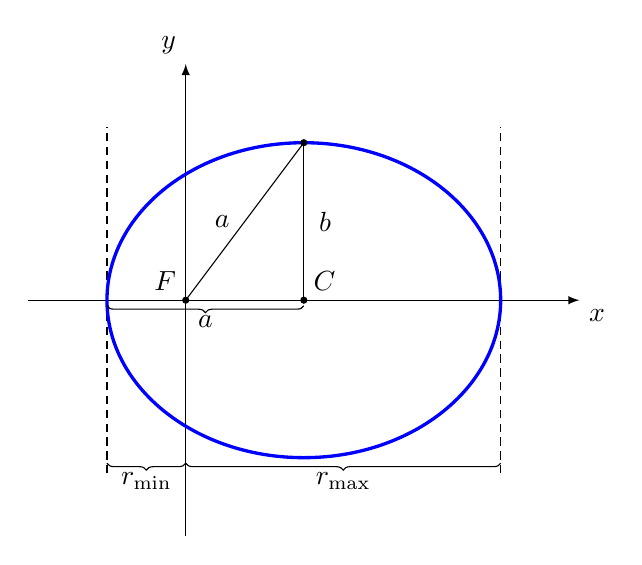
\begin{tikzpicture}
     \draw[-latex] (-2,0) -- (5,0) node[below right] {$x$};
     \draw[-latex] (0,-3) -- (0,3) node[above left] {$y$};
     \draw[densely dashed] (-1,-2.2) -- (-1,2.2);
     \draw[densely dashed] (4,-2.2) -- (4,2.2);
     \draw[blue,line width=1.2pt] (1.5,0) ellipse (2.5 and 2);
     \fill (1.5,0) circle (1.3 pt) node[above right] {$C$};
     \fill (0,0) circle (1.3 pt) node[above left] {$F$};
     \fill (1.5,2) circle (1.3 pt);
     \draw[decorate,decoration={brace,raise=2pt,mirror}] (-1,0) -- node[below=2pt]{$a$} (1.5,0);
     \draw (1.5,2) -- node[right=2pt]{$b$} (1.5,0);
     \draw (0,0) -- node[left=2pt]{$a$} (1.5,2);
     \draw[decorate,decoration={brace,mirror,raise=2pt}] (-1,-2) -- node[below=2pt]{$r_\text{min}$} (0,-2);
     \draw[decorate,decoration={brace,mirror,raise=2pt}] (0,-2) -- node[below=2pt]{$r_\text{max}$} (4,-2);
    \end{tikzpicture}
    \caption{A kapott ellipszispálya. A nagytengely hossza $a$ a kistengelyé $b$. Az origó az egyik fókusz ($F$), míg $C$ a centrum. Az origótól való legkisebb távolság $r_\text{min}$, a legnagyobb pedig $r_\text{max}$.}\label{fig:A13-ellipszis}
   \end{figure}
   Forgassuk el a koordináta-rendszert, hogy $\beta=0$ legyen. A legnagyobb és a legkisebb távolság, illetve a nagytengely hossza:
   \al{
    &r_\text{max}=\frac{p}{1-e}
    &r_\text{min}=\frac{p}{1+e}
    &&a=\frac{r_\text{max}+r_\text{min}}{2}
       =\frac{p}{1-e^2}.
   }
   A fókusz centrumtól mért távolsága, és a kistengely hossza:
   \al{
    &a-r_\text{min}=\frac{ep}{1-e^2}=e\cdot a.
    &b=\sqrt{a^2-(e\cdot a)^2}=\sqrt{a^2(1-e^2)}=\sqrt{a\cdot p},
   }
   amellyel a terület:
   \al{
    A=\pi ab =\pi\sqrt{a^3 p}.
   }
   A súrolt terület a területi sebesség és a periódusidő szorzataként is előáll (Kepler II{.}):
   \al{
    &\pi\sqrt{a^3 p}=T\cdot \frac{L}{2m}
    &\frac{T^2}{a^3}
      =\frac{4m^2\pi^2}{L^2}p
      =\frac{4m^2\pi^2}{L^2}\frac{L^2}{m\alpha}
      =\frac{4m\pi^2}{\alpha}
      =\text{állandó}.
   }
   Ez Kepler III.\ törvénye. Bolygómozgásnál $\alpha=mM\gamma$, így ott $\frac{T^2}{a^3}=\frac{4\pi^2}{M\gamma}$. A keringési idő bolygómozgásra:
   \al{
    T
    &=\sqrt{a^3\frac{4\pi^2}{M\gamma}}
     =\sqrt{\left(\frac{p}{1-e^2}\right)^3\frac{4\pi^2}{M\gamma}}
     =\sqrt{\left(\frac{\frac{L^2}{\gamma m^2 M}}{\frac{2\abs{E}L^2}{m\gamma^2 m^2 M^2}}\right)^3\frac{4\pi^2}{M\gamma}}
     =\sqrt{\left(\frac{m\gamma M}{2\abs{E}}\right)^3\frac{4\pi^2}{M\gamma}}\\
    &=\pi \gamma mM \sqrt{\frac{m}{2\abs{E}^3}}.
   }
 
 \section{Elektrodinamika} 
  
  \subsection{Coulomb-törvény kapcsolata a Maxwell-egyenletekkel}
   
   Lásd \ref{ss:01-CoulombMaxwell}. fejezet.
   
  \subsection{Oszcilláló töltéseloszlás tere}\label{ss:13-oszcillaloter}
   
   Tekintsünk olyan rendszert, ahol a potenciálok lokalizáltak (kiterjedése $d$), és szinuszosak: $\psi(\omega,\rv)$, $\Av(\omega,\rv)\sim e^{-i\omega t}$. Lorentz-mértékben: $0=\divo{\Av}+\frac{1}{c^2}\partial_t\phi=\divo{\Av}-\frac{1}{c^2}i\omega\phi$ így elég csak $\Av$-t kiszámítani, abból $\phi$ adódik.
   
   A retardált potenciálok (\ref{ss:9-retpot}. fejezet, illetve \eqref{eq:09-retpotA} egyenlet) szerint:
   \al{
    \vect{A}(t,\rv)
      &=\frac{\mu_0}{4\pi}\intl{}{}\dd^3\rv'\,\frac{\vect{J}\left(t-\frac{\abs{\rv-\rv'}}{c},\rv'\right)}{\abs{\rv-\rv'}}
       =\frac{\mu_0}{4\pi}\intl{}{}\dd^3\rv'\,\frac{\vect{J}(\rv')e^{-i\omega\left(t-\frac{\abs{\rv-\rv'}}{c}\right)}}{\abs{\rv-\rv'}}\\
    \vect{A}(\omega,\rv)
      &=\frac{\mu_0}{4\pi}\intl{}{}\dd^3\rv'\,\frac{\vect{J}(\rv')e^{ik\abs{\rv-\rv'}}}{\abs{\rv-\rv'}}
   }
   
   Közeltérben ($d\ll r\ll\lambda$), ahol $k\abs{\rv-\rv'}\ll 1$, nem számít a retardálás. A hullámzónában ($d\ll\lambda\ll r $) csak az $\sim\frac{1}{r}$ tagokat tartjuk meg:
   \al{
    \frac{1}{\abs{\rv-\rv'}}&=\frac{1}{r}+\mathcal{O}\left(\frac{d}{r^2}\right),\\
    \abs{\rv-\rv'}
      &=\sqrt{\rv^2-2\rv\rv'+\rv'^2}
      =r\sqrt{1-2\frac{\rv\rv'}{r^2}+\frac{\rv'^2}{\rv^2}}
      =r\sqrt{1-2\frac{\rv\rv'}{r^2}}+\mathcal{O}\left(\frac{d^2}{r}\right)\\
      &=r\left(1-\frac{\rv\rv'}{r^2}\right)+\mathcal{O}\left(\frac{d^2}{r}\right)
       =r-\rv'\ev_\rv+\mathcal{O}\left(\frac{d^2}{r}\right)\\
    e^{ik\abs{\rv-\rv'}}
      &\approx e^{ik(r-\rv'\ev_\rv)}
       =e^{ikr}e^{-ik\rv'\ev_\rv}
       \approx
        e^{ikr}\left(1-ik\rv'\ev_\rv\right),
   }
   az utolsó tagban felhasználtuk, hogy $k\abs{\rv'}<kd\ll 1$
   Így
   \aln{
    \vect{A}(\omega,\rv)
      &=\frac{\mu_0}{4\pi}\frac{e^{ikr}}{r}\intl{}{}\dd^3\rv'\,\vect{J}(\rv')\big(1-ik\rv'\ev_\rv\big)\label{eq:13-vectpot}
   }
    
   \paragraph{Mozgó töltés sugárzása}\label{ss:14-mogotoltessugarzasa}
    
    Tekintsünk egy ponttöltés, amely  általános mozgást végez: $\Jv(\rv)=q\vv(t)\delta\big(\rv-\vects{\gamma}(t)\big)$, ahol $\vects{\gamma}(t)$ a pálya. $\frac{1}{r}$-ed rendben \eqaref{eq:09-retpotA} egyenlet kiintegrálható:
    \al{
     \vect{A}(t,\rv)
      &\approx\frac{\mu_0}{4\pi}\intl{}{}\dd^3\rv'\,\frac{1}{r}q\vv(t)\delta\big(\rv'-\vects{\gamma}(t)\big)
       =\frac{\mu_0}{4\pi r}q\vv\left(t-\frac{r}{c}\right).
    }
    A deriválásnál is csak $\frac{1}{r}$-ed rendig tartjuk meg a tagokat, így $\vects{\nabla}\to-\frac{1}{c}\grad{r}\partial_t=-\frac{\rv}{rc}\partial_t=-\frac{\ev_\rv}{c}\partial_t$. A terek:
    \al{
     \Bv
      &=\rot{\Av}
       =\frac{q\mu_0}{4\pi}\rot{\vv\left(t-\frac{r}{c}\right)}
       =-\frac{q\mu_0}{4\pi c}\ev_\rv\times\partial_t\vv\left(t-\frac{r}{c}\right)
       =\frac{q\mu_0}{4\pi r c}\left[\av\left(t-\frac{r}{c}\right)\times\ev_\rv\right]  \\
     \dot{\Ev}
      &=c^2\rot{\Bv}
       =c^2\frac{q\mu_0}{4\pi r^2 c^2}\left[\dot{\av}\left(t-\frac{r}{c}\right)\times\ev_\rv\right]\times\ev_\rv\\
     \Ev
      &=\frac{q\mu_0}{4\pi r^2 }\left[\av\left(t-\frac{r}{c}\right)\times\ev_\rv\right]\times\ev_\rv
       =Z_0\Hv\times\ev_\rv.
    }
    A kisugárzott teljesítménysűrűség:
    \al{
     \Sv
      &=\Ev\times\Hv
       =Z_0(\Hv\times\ev_\rv)\times\Hv
       =Z_0\Hv^2\ev_\rv
       =Z_0\frac{q^2}{16\pi^2 r^2 c^2}\left[a\left(t-\frac{r}{c}\right)\right]^2\sin^2\vartheta\ev_\rv,
    }
    ahol $Z_0=\mu_0 c$ a vákuum ellenállása. Innen
    \aln{
     &\der{P}{\Omega}=\frac{Z_0 q^2}{16\pi^2 c^2}\left[a\left(t-\frac{r}{c}\right)\right]^2\sin^2\vartheta,
     &P=\frac{Z_0 q^2}{6\pi c^2}\left[a\left(t-\frac{r}{c}\right)\right]^2.\label{eq:13-Larmor}
    }
    Ez a Larmor-képlet. Látjuk, hogy a gyorsuló töltés sugároz. A képlet akkor használható, ha $d\ll \lambda\Leftrightarrow \frac{d}{\delta t}\ll \frac{\lambda}{\delta t}\Leftrightarrow v\ll c$, vagyis a nem relativisztikus határesetben.
    
    Körmozgásra $a\left(t-\frac{r}{c}\right)=\frac{v^2}{R}$:
    \al{
     P=\frac{Z_0 q^2}{6\pi c^2}\frac{v^4}{R^2}
      =\frac{Z_0 q^2 c^2}{6\pi R^2}\left(\frac{v}{c}\right)^4.
    }
    
   \paragraph{Sugárzás relativisztikus tárgyalása, Ciklotron sugárzás} 
    
    A relativisztikus tárgyaláshoz a Larmor-képletet relativisztikusan invariáns alakban kell felírni.
     
    A bal oldalon a teljesítmény $P=\der{E}{t}$, melyhez álló rendszerben $c\minv{p}^\mu=(E,0)$, és $\minv{x}^\mu=(ct,0)$. Mozgó rendszerbe való áttérésnél: $E\to E'=\frac{E}{\sqrt{1-v^2/c^2}}$ és $t\to t'=\frac{t}{\sqrt{1-v^2/c^2}}$, ahonnan: $\det{E}{t}=\der{E'}{t'}$, vagyis invariáns. 
    
    A jobb oldalon $\vect{a}$ nem kovariáns. A $v\to 0$ limesz ismeretében azzá tehetjük:
    \al{
     \minv{a}^\mu
      &=\der{^2\minv{r}^\mu}{^2\tau}
       =\der{}{\tau}\left(\frac{c}{\sqrt{1-\frac{v^2}{c^2}}},\frac{\vv}{\sqrt{1-\frac{v^2}{c^2}}}\right)
       =\frac{1}{\sqrt{1-\frac{v^2}{c^2}}^2}\left(0,\av\right)
        +\left(c,\vv\right)\der{}{\tau}\frac{1}{\sqrt{1-\frac{v^2}{c^2}}}\\
      &=\frac{1}{\sqrt{1-\frac{v^2}{c^2}}^2}\left(0,\av\right)
        +\frac{\vv\av}{c^2}\frac{1}{\sqrt{1-\frac{v^2}{c^2}}^4}\left(c,\vv\right)
       =\left(\frac{\vects{\beta}\av}{\sqrt{1-\frac{v^2}{c^2}}^4},\frac{\av}{\sqrt{1-\frac{v^2}{c^2}}^2}+\frac{(\vects{\beta}\av)\vects{\beta}}{\sqrt{1-\frac{v^2}{c^2}}^4}\right)\\
      &=\big(\gamma^4\vects{\beta}\av,\gamma^2\av+(\vects{\beta}\av)\vects{\beta}\gamma^4\big),
    }
    ami tudja, hogy $\minv{a}^\mu\to (0,\av)$, illetve $\minv{a}^\mu \minv{a}_\mu\to -\av^2$. Ezzel a Larmor-képlet felírva:
    \al{
     P=-\frac{Z_0 q^2}{6\pi c^2}\minv{a}^\mu \minv{a}_\mu,
    }
    szembeötlően invariáns. Visszaírjuk a gyorsulást és a sebességet:
    \al{
     \minv{a}^\mu\minv{a}_\mu
     &=\gamma^8(\vects{\beta}\av)^2-\gamma^4\av^2-(\vects{\beta}\av)^2\vects{\beta}^2\gamma^8-2\gamma^6(\vects{\beta}\av)^2\\
     &=-\gamma^4\av^2-\gamma^6(\vects{\beta}\av)^2+\gamma^6(\vects{\beta}\av)^2\Big[\underbrace{\gamma^2\big(1-\vects{\beta}^2\big)}_{=1}-1\Big]
      =-\gamma^4\av^2-\gamma^6(\vects{\beta}\av)^2.
    }
    Ez $\vv\to 0$-ra, visszaadja $-\av^2$-et, így a fenti kifejezés megfelel a klasszikus határesetnek. Alakítsuk még egy kicsit:
    \al{
     \minv{a}^\mu\minv{a}_\mu
      &=-\gamma^4\av^2-\gamma^6(\vects{\beta}\av)^2
       =-\gamma^6\big[(1-\betav^2)\av^2+(\vects{\beta}\av)^2\big]
       =-\gamma^6\big[\av^2+(\vects{\beta}\av)^2-\av^2\betav^2\big]\\
      &=-\gamma^6\big[\av^2+(\vects{\beta}\times\av)^2\big].
    }
    Ezzel tehát a Larmor-formula relativisztikus megfelelője:
    \al{
     P=\frac{Z_0 q^2}{6\pi c^2}\gamma^6\big[\av^2+(\vects{\beta}\times\av)^2\big].
    }
    Körmozgás esetén $\betav\perp\av$, így $(\vects{\beta}\times\av)^2=a^2\beta^2$, vagyis:
    \al{
     P=\frac{Z_0 q^2}{6\pi c^2}\gamma^6\big[(1-\beta^2)a^2\big]
      =\frac{Z_0 q^2}{6\pi c^2}\gamma^4 a^2.
    }
    A klasszikus képletet képest ez egy $\gamma^4$-es faktorban tér el. Ha $v\sim c$, akkor a sugárzás teljesítménye nagyon megnő.
    
    
 \section{Kvantummechanika}
  
  \subsection{Kötött állapot} 
   
   Kötött állapotról akkor beszélünk, ha a rendszer spektruma pontspektrum. Ekkor a hullámfüggvény normálható, és az eleme a négyzetesen integrálható függvények Hilbert-terének.
   
  \subsection{Schrödigner-egyenlet centrális erőtérben}
   
   Legyen a potenciál centrális, azaz $\opV(\oprv)=\opV(\opr)$. Ekkor a Schrödinger-egyenlet gombi koordinátákban, koordinátareprezentációban:
   \al{
    \left\{-\frac{\hbar^2}{2m}\left[\frac{1}{r}\partial_r^2r+\frac{1}{r^2}\left(\partial_{\vartheta}+\frac{1}{\tg{\vartheta}}\partial_{\vartheta}^2+\frac{1}{\sin^2{\varphi}}\partial_{\vartheta}^2\right)\right]+V(r)\right\}\psi(r,\vartheta,\varphi)=E\psi(r,\vartheta,\varphi).
   }
   Az 
   \al{
    L^2=-\hbar^2\left(\partial_{\vartheta}^2+\frac{1}{\tg{\vartheta}}\partial_{\vartheta}+\frac{1}{\sin^2{\vartheta}}\partial_{\varphi}^2\right)
   }
   sajátérték problémájának megoldását lásd \ref{ss:06-L2spme}. fejezet. A megoldást akkor keressük
   \al{
    \psi(r,\vartheta,\varphi)=\frac{1}{r}R(r)Y_l^m(\vartheta,\varphi)
   }
   alakban, melyet behelyettesítve az egyenletbe a radiális Schrödinger-egyenletet kapjuk:
   \aln{
    \left[-\frac{\hbar^2}{2m}\frac{1}{r}\partial_r^2r+\frac{\hbar^2 l(l+1)}{2mr^2}+V(r)\right]\psi(r,\vartheta,\varphi)&=E\psi(r,\vartheta,\varphi)\nonumber\\
    \left[-\frac{\hbar^2}{2m}\der{^2}{r^2}+\frac{\hbar^2 l(l+1)}{2mr^2}+V(r)\right]R(r)&=ER(r).\label{eq:13:radSch}
   }
   
  \subsection{Hidrogénatom}
   
   Legyen $V(r)=-\frac{kZe^2}{r}$. Az állapotok negatív energiájúak: $E=-\abs{E}$. Ezzel az egyenlet:
   \al{
    0=\left[-\frac{\hbar^2}{2m}\der{^2}{r^2}+\frac{\hbar^2 l(l+1)}{2mr^2}-\frac{kZe^2}{r}+\abs{E}\right]R(r).
   }
   Bevzetjük az alábbi jelöléseket:
   \al{
    &r_0=\frac{\hbar}{\sqrt{2m\abs{E}}}
    &\xi=\frac{\sqrt{8m\abs{E}}}{\hbar}r=\frac{2r}{r_0}
    &&a_0=\frac{\hbar^2}{mke^2}
    &&\ep=\frac{Zke^2\sqrt{2m\abs{e}}}{2\hbar\abs{E}},
   }
   melyekkel
   \al{
    \der{^2R(\xi)}{\xi^2}+\left[-\frac{1}{4}+\frac{\ep}{\xi}-\frac{l(l+1)}{\xi^2}\right]R(\xi)=0.
   }
   
   \paragraph{Sommerfeld polinommódszer}
    
    Először megkeressük az aszimptotikus megoldást:
    \al{
     &\xi\to 0
     &\der{^2R(\xi)}{\xi^2}-\frac{l(l+1)}{\xi^2}R(\xi)=0
     &&R(\xi)\sim\xi^{l+1},\\
     &\xi\to \infty
     &\der{^2R(\xi)}{\xi^2}-\frac{1}{4}R(\xi)=0
     &&R(\xi)\sim e^{-\frac{1}{2}\xi}.
    }
    
    A megoldást keressük egy polinom és az aszimptotikus megoldás szorzataként: $R(\xi)=u(\xi)e^{-\frac{1}{2}\xi}$, mellyel
    \al{
     &\dd_\xi R(\xi)=\left(-\frac{1}{2}u(\xi)+u'(\xi)\right)e^{-\frac{1}{2}\xi}
     &\dd_\xi^2 R(\xi)=\left(\frac{1}{4}u(\xi)-u'(\xi)+u''(\xi)\right)e^{-\frac{1}{2}\xi},
    }
    így
    \al{
     u''(\xi)-u'(\xi)+\left[\frac{\ep}{\xi}-\frac{l(l+1)}{\xi^2}\right]u(\xi)=0.
    }
    A hatványsor legyen $u(\xi)=\xi^s\suml{i=0}{\infty}c_i\xi^i$, ahol $s$ az iniciális index. Ennek deriváltjai:
    \al{
     u'(\xi)&=\suml{i=0}{\infty}(i+s)c_i\xi^{i+s-1}
      =\suml{i=1}{\infty}(i+s-1)c_{i-1}\xi^{i+s-2}\\
     u''(\xi)&=\suml{i=0}{\infty}(i+s)(i+s-1)c_i\xi^{i+s-2},
    }
    majd behelyettesítve:
    \al{
     0
      &=\suml{i=0}{\infty}(i+s)(i+s-1)c_i\xi^{i+s-2}-\suml{i=1}{\infty}(i+s-1)c_{i-1}\xi^{i+s-2}+\left[\frac{\ep}{\xi}-\frac{l(l+1)}{\xi^2}\right]\suml{i=0}{\infty}c_{i}\xi^{i+s}\\
      &=s(s-1)c_0\xi^{s-2}+\suml{i=1}{\infty}\bigg(
       (i+s)(i+s-1)c_i\xi^{i+s-2}
      -(i+s-1)c_{i-1}\xi^{i+s-2}\bigg)\\
      &\qquad\qquad\qquad+\suml{i=0}{\infty}\left[\ep c_{i}\xi^{i+s-1}-l(l+1)c_{i}\xi^{i+s-2}\right]\\
      &=\big[s(s-1)-l(l+1)\big]c_0\xi^{s-2}+\suml{i=1}{\infty}\bigg(
        \big[(i+s)(i+s-1)-l(l+1)\big]c_i\\
      &\qquad\qquad\qquad\qquad\qquad\qquad\qquad\qquad\qquad\qquad\qquad\qquad
        +\big[\ep-(i+s-1)\big]c_{i-1}\bigg)\xi^{i+s-2}.
    }
    Ennek mindegyik együtthatója el kell, hogy tűnjön. $c_0\ne 0$, mert biztos van egy olyan $c_i$, így $s=l+1$ vagy $s=-l$, ahonnan csak az első jön szóba, a $\xi\to 0$-ban való regularitás miatt. A többi együtthatóra:
    \al{
     c_i
      =\frac{-\ep+(i+s-1)}{(i+s)(i+s-1)-l(l+1)}c_{i-1}
      =\frac{-\ep+i+l}{i(i+2l+1)}c_{i-1}.
    }
    Nagy $i$-re $\frac{c_i}{c_{i-1}}\sim\frac{1}{i}$, ami így azt eredményezné, hogy $u\sim e^{\xi}$, vagyis $R(\xi)\sim e^{\frac{1}{2}\xi}$, ami nem reguláris. Emiatt léteznie kell egy $i_\text{max}$-nak, hogy $c_{i_\text{max}}=0$. Ekkor 
    \al{
     i_\text{max}+l-\ep=0.
    }
    Bevezetjük az
    \al{
     n=i_\text{max}+l=\ep,
    }
    főkvantumszámot, ami: $n>l$, $n=1,2,3,\dots$, illetve $n=\frac{Z r_0}{a_0}$. Az eredmény összefoglalva:
    \al{
     E_n
      &=-\frac{\hbar^2}{2m r_0^2}
       =-\frac{Z^2\hbar^2}{2m a_0^2}\frac{1}{n^2}
       =-\frac{mZ^2 k^2e^4}{2\hbar^2}\frac{1}{n^2}
       =-\frac{mZ^2e^4}{32\pi^2\ep_0^2\hbar^2}\frac{1}{n^2},
    }
    \al{
     \psi(r,\vartheta,\varphi)
      &=
       \sqrt{{\left (\frac{2}{r_0} \right ) }^3\frac{(n-l-1)!}{2n\,(n+l)!} } 
       \left(\frac{2r}{r_0}\right)^l L_{n-l-1}^{2l+1}\left(\frac{2r}{r_0}\right)e^{-\frac{r}{r_0}}Y_l^m(\vartheta,\varphi),
    }
    ahol $L_{n-l-1}^{2l+1}\left(\frac{2r}{r_0}\right)$ az asszociált Laguerre-polinomok:
    \al{
     L_n^{\alpha}(x)=\frac{x^{-\alpha} e^x}{ n!}\frac{d^n}{dx^n} \left(e^{-x} x^{n+\alpha}\right).
    }
    \begin{figure}[ht!]
     \centering
    \subfloat[$n=1$\label{fig:A13-e1}]{\includegraphics[width= 0.3\textwidth]{./A13tetel/H-n1}} \hspace{6pt}
    \subfloat[$n=2$\label{fig:A13-e2}]{\includegraphics[width= 0.3\textwidth]{./A13tetel/H-n2}} \hspace{6pt}
    \subfloat[$n=3$\label{fig:A13-e3}]{\includegraphics[width= 0.3\textwidth]{./A13tetel/H-n3}}
     \caption{Radiális valószínűségek ($w_{n,l}(r)=\abs{\Psi_r(r)}^2\cdot r^2$) az első három energiaszinthez tartozó hullámfüggvények esetében. (Az $y$ tengely skálája változik az ábrákon!)}
    \end{figure}
    
%     \al{
%      L_{n-l-1}^{2l+1}\left(\frac{r}{2r_0}\right)=\frac{\left(\frac{r}{2r_0}\right)^{-(2l+1)} e^{\frac{r}{2r_0}}}{ (n-l-1)!}\frac{\dd^{n-l-1}}{\dd \left(\frac{r}{2r_0}\right)^{n-l-1}} \left(e^{-\frac{r}{2r_0}} \left(\frac{r}{2r_0}\right)^{(n-l-1)+(2l+1)}\right).
%     }
    
    
    
    
    

  \chapter{Mozg\'as centr\'alis er\H{o}t\'erben: Sz\'or\'asi folyamatok}
 
 \section{Mechanika} 
  
  \subsection{Kéttestprobléma} 
   
   Vizsgáljunk két tömegponttot, amelyek csak egymásra hatnak. A mozgásegyenletek:
   \al{
    &m_1\ddot\rv_1=\Fv_{12}
    &m_2\ddot\rv_2=\Fv_{21}
    &&\Fv_{12}=-\Fv_{21}.
   }
   A két egyenlet összege: $0=\dd_t^2(m_1\rv_1+m_2\rv_2)$, vagyis az $\Rv=\frac{m_1\rv_1+m_2\rv_2}{m_1+m_2}$ pont egyenes vonalú egyenletes mozgást végez. Ez a tömegközéppont megmaradásának tétele. Rögzítsük az origót ehhez a ponthoz. Ekkor $m_1\rv_1+m_2\rv_2=0$.
   
   Vezessük le a különbségi koordinátára ($\rv=\rv_2-\rv_1$) egy mozgásegyenletet. A két mozgásegyenletet a másik tömegekkel bővítve majd kivonva:
   \al{
    m_1 m_2(\ddot\rv_2-\ddot\rv_1)&=-m_2\Fv_{21}+m_1\Fv_{12}=(m_1+m_2)\Fv_{12}\\
    \frac{m_1 m_2}{m_1+m_2}\ddot\rv&=\Fv_{12}.
   } 
   ahol $\mu=\frac{m_1 m_2}{m_1+m_2}$ a redukált tömeg. A problémát visszavezettük egy egyrészecske problémára. A tömegközépponti rendszerben a két tömegpont koordinátája ezzel:
   \al{
    &\rv_1=-\rv\frac{m_2}{m_1+m_2}
    &\rv_2=\rv\frac{m_1}{m_1+m_2}.
   } 
   
   Ezzel pl. a Kepler-probléma esetében figyelembe vehető, hogy a Nap nem rögzített. A kapott eredményben szereplő $m$ nem a Föld tömege, hanem a redukált tömeg. 
   
  \subsection{Szórásszámítás}
   
   Legyen az origóban egy szórócentrum, amely által létrehozott centrális potenciálban mozog a szóródó részecske. Aszimptotikus távolságban a mozgás egyenes vonalú egyenletes. Kérdés, hogy mekkora lesz a szórás után aszimptotikus távolságban a kilépő részecske pályájának elhajlása a bemenő pályához képest. 
   
   A mozgás során megmaradó mennyiségek:
   \begin{itemize}
    \item az energia, ha az ütközés rugalmas,
    \item az összimpulzus, ha nincs külső erő,
    \item a impulzusmomentum
    \item a tömegkközéppont.
   \end{itemize}
   
   A beérkező részecske energiája aszimptotikus távolságban: $E=\frac{1}{2}m^2 v_\infty^2$, impulzusmomentuma $L=m\rho v_\infty$, ahol $\rho$ az asziptotikus pálya és az origó távolsága. $\rho$ az ütközési paraméter, ettől függ, hogy milyen $\chi$ szögben fog szóródni a kilépő részecske. A $\rho(\chi)$ függvényt keressük meg. 
   
   A belépő részecskefluxus $n$ (darab/felület/másodperc), mellyel a részecskeáram (da\-rab/má\-sod\-perc) a $\rho$ sugarú $\dd\rho$ széles gyűrűn: $\dd N=n2\pi\rho\dd\rho$. Ezek a részecskék fognak ugyanabba a $\chi$ szögbe szóródni. A térszög, ami ehhez tartozik: $\dd\Omega=\frac{1}{r^2}2\pi r\sin\chi r\dd\chi=2\pi\sin\chi\dd\chi$. Bevezetjük azt az arányt, ami azt jellemzi, hogy a részecskék mekkora része szóródik $\dd\chi$ szögben:
   \aln{
    \dd\sigma
     =\frac{\dd N}{n}
     =2\pi\rho\dd\rho
     =2\pi\rho\abs{\der{\rho}{\chi}}\dd\chi
     =2\pi\rho\abs{\der{\rho}{\chi}}\frac{\dd\Omega}{2\pi\sin\chi}
     =\frac{\rho}{\sin\chi}\abs{\der{\rho}{\chi}}\dd\Omega.\label{eq:14-dhatkm}
   }
   A $\der{\sigma}{\Omega}$ a differenciális szórási hatáskeresztmetszet, mértékegysége $\mathrm{m}^2$. 
   
   \paragraph{Példa: tömör, $R$ sugarú gömb}
    
    Szórás akkor történik, ha $\rho\leq R$. Ekkor a szórás szöge $\chi$, ami a beesés szögével kifejezhető $\chi=\pi-2\varphi$. 
    \al{
     \rho
      =R\sin\varphi
      =R\sin\left(\frac{\pi-\chi}{2}\right)
      =R\cos\left(\frac{\chi}{2}\right).
    }
    Ezzel
    \al{
     \der{\sigma}{\Omega}
      =\frac{\rho}{\sin\chi}\abs{\der{\rho}{\chi}}
      =\frac{R\cos\left(\frac{\chi}{2}\right)}{\sin\chi}\abs{\der{}{\chi}R\cos\left(\frac{\chi}{2}\right)}
      =\frac{R^2}{2}\frac{\cos\left(\frac{\chi}{2}\right)}{\sin\chi}\sin\left(\frac{\chi}{2}\right)
      =\frac{R^2}{4}\frac{\sin\left(\chi\right)}{\sin\chi}
      =\frac{R^2}{4},
    }
    így
    \al{
     \sigma=\frac{R^2}{4}\cdot 4\pi=R^2\pi.
    } 
    Tehát a gömb szórási hatáskeresztmetszete megegyezik a gömb keresztmetszetével.
    
  \subsection{Rutherford szórás}
   
   Lásd \aref{ss:13-palyaegyenlete}. fejezetben. A lehetséges pályákat \aref{fig:A14-palyak}. ábra mutatja.
   
   \begin{figure}[ht!]
    \centering
    \includegraphics[width=0.35\textwidth]{A14tetel/palyak}
    \caption{A szórócentrum az origóban van. Vonzó kölcsönhatás esetén a bal oldali hiperbola ág mutatja a pályát. Taszító kölcsönhatás esetén a jobb oldali pálya valósul meg. Az ütközési paraméter ($\rho$) a két aszimptota távolsága az origótól.}\label{fig:A14-palyak}
   \end{figure}

   
   Rögzítjük a $q_1$ töltést, $q_2$ töltést pedig szóratjuk a $q_1$ terén. Legyen a töltés taszító, ekkor $\alpha=-k q_1 q_2$. Ekkor a hiperbola megfordul, így az egyenlete:
   \al{
    &r(\varphi)=\frac{-\abs{p}}{1-e\cos(\varphi)}
    &p=\frac{L^2}{m\alpha}=-\frac{m v_\infty^2 \rho^2}{\abs{\alpha}}
    &&e=\sqrt{1+\frac{2EL^2}{m\alpha^2}}
%        =\sqrt{1+\frac{m v_\infty^2 m v_\infty^2 \rho^2}{m\alpha^2}}
       =\sqrt{1+\left(\frac{m  \rho v_\infty^2}{\alpha}\right)^2}.
   }
   
   A két aszimptota a $\varphi_{1,2}=\pm\arccos{\frac{1}{e}}$-nél van, így a szórási szög:
   \al{
    \chi
     &=\pi-(\varphi_1-\varphi_2)
      =\pi-2\arccos\frac{1}{e}
      =2\left(\frac{\pi}{2}-\arccos\frac{1}{e}\right)
      =2\arcsin\frac{1}{e}\\
    \sin\frac{\chi}{2}
     &=\frac{1}{e}
      =\frac{1}{\sqrt{1+\left(\frac{m  \rho v_\infty^2}{\alpha}\right)^2}}\\
     \rho(\chi)
      &=\frac{\abs{\alpha}}{m v_\infty^2}\sqrt{\frac{1}{\sin^2\frac{\chi}{2}}-1}
       =\frac{\abs{\alpha}}{m v_\infty^2}\frac{1}{\tg\frac{\chi}{2}},
   }
   ahonnan a differenciális hatáskeresztmetszet:
   \al{
    \der{\sigma}{\Omega}
     &=\frac{\rho}{\sin\chi}\abs{\der{\rho}{\chi}}
      =\frac{\alpha^2}{m^2 v_\infty^4}\frac{1}{\sin\chi}\frac{1}{\tg\frac{\chi}{2}}\abs{\der{}{\chi}\frac{1}{\tg\frac{\chi}{2}}}
      =\frac{\alpha^2}{m^2 v_\infty^4}\frac{1}{\sin\chi}\frac{1}{\tg\frac{\chi}{2}}\frac{1}{2}\frac{1}{\sin^2\frac{\chi}{2}}\\
     &=\frac{\alpha^2}{m^2 v_\infty^4}\frac{1}{2\sin^2\frac{\chi}{2}}\frac{1}{2}\frac{1}{\sin^2\frac{\chi}{2}}
      =\left(\frac{\alpha}{2m v_\infty^2}\right)^2\frac{1}{\sin^4\frac{\chi}{2}},
   }
   melyből a teljes szórási hatáskeresztmetszet:
   \al{
    \sigma
     &=\intl{}{}\dd\Omega\,\left(\frac{\alpha}{2m v_\infty^2}\right)^2\frac{1}{\sin^4\frac{\chi}{2}}
      =\left(\frac{\alpha}{2m v_\infty^2}\right)^2\intl{0}{\pi}\dd\chi\,2\pi\sin\chi\frac{1}{\sin^4\frac{\chi}{2}}\\
     &=\left(\frac{\alpha}{2m v_\infty^2}\right)^2 4\pi\intl{0}{\pi}\dd\chi\,\frac{\cos\frac{\chi}{2}}{\sin^3\frac{\chi}{2}}
      =\left(\frac{\alpha}{2m v_\infty^2}\right)^2 4\pi\left[-\frac{1}{\sin^2\frac{\chi}{2}}\right]_{0}^{\pi}
      =\text{divergens!}
   }
   
   Ez nem meglepő, a Coulomb-potenciál $\sim\frac{1}{r}$-es, azaz végtelen hatótávolságú. A kísérleti eredményekkel ez ott egyeztethető össze, hogy itt nem vettük figyelembe az árnyékolást, pl. szilárdtestekben való szóródásnál a szóró potenciálra sokkal reálisabb közelítés a $\sim\frac{e^{-r/r_0}}{r}$ alak, aminek hatótávolsága véges, így szórási hatáskeresztmetszete is az.
   
   Megjegyzés: a kvantummechanikai szóráselmélet is a Rutherford-féle formulát adja, a differenciális hatáskeresztmetszetre levezetett összefüggés a kvantummechanikában is helytálló. 
   
 \section{Kvantummechanika}
  
  \subsection{Potenciálszórás}
   
   A kéttest ütközések visszavezethetőek egyrészecske problémára, így a szórásokat úgy vizsgáljuk, hogy egy részecskét szóratunk fix potenciálon. A kísérletileg mérhető differenciális hatáskeresztmetszetet szeretnénk meghatározni a rendszer tulajdonságaiból.
   
   Essen egy monokromatikus $\kv_i$ hullámszámú részecske a szórócentrumra. A potenciál legye rövid hatótávolságú, vagyis $V(\rv)\sim\frac{1}{r^{1+\ep}}$, ahol $\ep>0$. A radiális Schrödinger-egyenlet $r\to\infty$ aszimptotikus megoldása $\mathcal{O}\left(\frac{1}{r}\right)$ rendig:
   \aln{
    \psi(k,\rv)=A\bigg(\underbrace{e^{i\kv_i\rv}}_{\text{be}}+\underbrace{f(\vartheta,\varphi)\frac{e^{i k r}}{r}}_{\text{szórt}}\bigg)
     =\psi_\text{be}(\rv)+\psi_\text{ki}(\rv,k),\label{eq:14-aszimptotikuspsi}
   }
   aminek az első tagja a beeső $\kv_i$ impulzusú síkhullám, a második tagja pedig egy kifutó gömbhullám.
   
   Számoljuk ki a detektoron ($r\to\infty$) a szórási folyamat nélkül beeső hullám, illetve a szórócentrum jelenlétében mérhető részecskeáram-sűrűségének hányadosát. Ebből a deifferenciális haráskeresztmetszet számolható lesz.
   
   A részecskeáram-sűrűség:
   \al{
    \jv(\rv)
     &=\Re\left[\frac{\hbar}{mi}\psi^*(\rv)\grad{\psi(\rv)}\right],
   }
   ahol $\grad=\frac{\partial }{\partial r}\ev_r+\frac{1}{r}\frac{\partial }{\partial \vartheta}\ev_\vartheta+\frac{1}{r \sin\vartheta}\frac{\partial }{\partial \phi}\ev_\varphi\xrightarrow{r\to\infty}\frac{\partial }{\partial r}\ev_r$, így
   \al{
    \jv(\rv)
%      &=\frac{\hbar}{mi}\Re\left[\left(e^{i\kv_i\rv}+f(\vartheta,\varphi)\frac{e^{i\kv\rv}}{r}\right)\frac{\partial }{\partial r}\ev_r\left(e^{i\kv_i\rv}+f(\vartheta,\varphi)\frac{e^{i\kv\rv}}{r}\right)\right],
     &=\Re\left[\frac{\hbar}{mi}\big(\psi^*_\text{be}(\rv)+\psi^*_\text{ki}(\rv,k)\big)\frac{\partial }{\partial r}\ev_r\big(\psi_\text{be}(\rv)+\psi_\text{ki}(\rv,k)\big)\right]\\
     &=\underbrace{\Re\left[\frac{\hbar}{mi}\psi^*_\text{be}(\rv)\grad\psi_\text{be}(\rv)\right]}_{\jv_\text{be}(\rv)}
      +\underbrace{\Re\left[\frac{\hbar}{mi}\psi^*_\text{ki}(\rv,k)\frac{\partial }{\partial r}\psi_\text{ki}(\rv,k)\right]}_{j_\text{sz}(\rv)}\ev_r\\
     &\qquad\qquad+\underbrace{\Re\left[\frac{\hbar}{mi}\left(\psi^*_\text{be}(\rv)\frac{\partial }{\partial r}\psi_\text{ki}(\rv,k)+\psi^*_\text{ki}(\rv,k)\frac{\partial }{\partial r}\psi_\text{be}(\rv)\right)\right]}_{j_\text{interf}(\rv)}\ev_r,
   }
   ahol a $z$ tengely párhuzamos $\kv_i$-vel, így $\kv_i\rv=k_i r\cos\vartheta$. Fejtsük ki a tagokat:
   \al{
    \jv_\text{be}
     &=\Re\left[\frac{\hbar}{mi}A^*\big(e^{-i\kv_i\rv}\big)\grad\big(Ae^{i\kv_i\rv}\big)\right]
      =\Re\left[\frac{\hbar}{mi}\abs{A}^2i\kv_i\right]
      =\abs{A}^2\frac{\hbar\kv_i}{m}
      =\abs{A}^2 \vv_i\\
    \jv_\text{sz}
     &=\Re\left[\frac{\hbar}{mi}\bigg(A^* f^*(\vartheta,\varphi)\frac{e^{-i k r}}{r}\bigg)\frac{\partial }{\partial r}\bigg(A f(\vartheta,\varphi)\frac{e^{i k r}}{r}\bigg)\right]\ev_r\\
     &=\abs{A}^2\Re\left[\frac{\hbar}{mi}\bigg(f^*(\vartheta,\varphi)\frac{e^{-i k r}}{r}\bigg)\bigg(f(\vartheta,\varphi)\partial_r \frac{e^{i k r}}{r}\bigg)\right]\ev_r\\
     &=\abs{A}^2\Re\left[\frac{\hbar}{mi}\bigg(f^*(\vartheta,\varphi)\frac{e^{-i k r}}{r}\bigg)\bigg(f(\vartheta,\varphi)ik\frac{e^{i k r}}{r}\bigg)\right]\ev_r+\mathcal{O}\left(\frac{1}{r^3}\right)\\
     &=\abs{A}^2\abs{f(\vartheta,\varphi)}^2\Re\left[\frac{\hbar}{mi} i k\frac{1}{r^2}\right]+\mathcal{O}\left(\frac{1}{r^3}\right)
      =\abs{A}^2v\ev_r\frac{1}{r^2}\abs{f(\vartheta,\varphi)}^2+\mathcal{O}\left(\frac{1}{r^3}\right)\\
    \jv_\text{interf}
     &=\abs{A}^2\Re\left[\frac{\hbar}{mi}\left(e^{-i\kv_i\rv}\frac{\partial }{\partial r}f(\vartheta,\varphi)\frac{e^{i k r}}{r}+f^*(\vartheta,\varphi)\frac{e^{-i k r}}{r}\frac{\partial }{\partial r}e^{i\kv_i\rv}\right)\right]\ev_r\\
     &=\abs{A}^2\Re\left[\frac{\hbar}{mi}\left(e^{-i\kv_i\rv}f(\vartheta,\varphi)i k\frac{e^{i k r}}{r}+f^*(\vartheta,\varphi)\frac{e^{-i k r}}{r}ik_i\cos\vartheta e^{i\kv_i\rv}\right)\right]\ev_r+\mathcal{O}\left(\frac{1}{r^2}\right).
   }   
   Tegyük fel hogy a szórás rugalmas, azaz $k_i=k$, illetve $v_i=v$, ekkor:
   \al{
    \jv_\text{interf}
     &=\abs{A}^2\frac{1}{r}\Re\left[\frac{\hbar}{mi}\left(ik f(\vartheta,\varphi)e^{i k r(1-\cos\vartheta)}+ikf^*(\vartheta,\varphi)\cos\vartheta e^{-i k r(1-\cos\vartheta)}\right)\right]\ev_r+\mathcal{O}\left(\frac{1}{r^2}\right),
   }
   ami $k$ hulámszámmal oszcillál, amit nem tud a detektor felbontani, így kiátlagolódik. Egyedül akkor nem tűnik el ez a tag, ha $\vartheta=0$.
   
   Innen a differenciális hatáskeresztmetszet \eqaref{eq:14-dhatkm} alapján: $\der{\sigma}{\omega}=\frac{\dd N}{n\dd\Omega}$. Itt $\dd N$ a detektorra érkező részecskeáram és $n$ a forrásból kijövő részecskeáram-sűrűség. Ez a hányados megegyezik a detektorra eső valószínűségi áram $j_\text{sz}A=j_\text{sz}r^2\dd\Omega$ és a bejövő valószínűségi áramsűrűség, vagyis $j_\text{be}$ hányadosával. Behelyettesítve:
   \aln{
    \der{\sigma}{\Omega}
     =\frac{\dd N}{n\dd\Omega}
     =\frac{j_\text{sz}r^2\Omega}{j_\text{be}\dd\Omega}
     =\frac{j_\text{sz}r^2}{j_\text{be}}
     =\frac{\abs{A}^2v\frac{1}{r^2}\abs{f(\vartheta,\varphi)}^2r^2}{\abs{A}^2 v}
     =\abs{f(\vartheta,\varphi)}^2.\label{eq:14-sigma-f}
   }
   
  \subsection{Optikai tétel}
   
   A $\vartheta=0$ esetben az interferencia tag nem hagyható el, az lesz a jelentős. Számítsuk ki egy $\delta\vartheta\to 0$ szögtartományra a részecskeáramot. 
   \al{
    &I_\text{interf}(\delta\vartheta\to 0)\\
    \qquad&=\intl{}{\delta\Omega}\dd\,\Omega r^2 \jv_\text{interf}\ev_r
     =\intl{0}{2\pi}\dd\varphi\intl{0}{\delta\vartheta}\dd\vartheta \sin\vartheta r^2 \jv_\text{interf}\ev_r\\
    \qquad&=\intl{0}{2\pi}\dd\varphi\intl{0}{\delta\vartheta}\dd\vartheta\,\sin\vartheta r^2\abs{A}^2\frac{1}{r}\Re\left[\frac{\hbar}{mi}\left(ik f(\vartheta,\varphi)e^{i k r(1-\cos\vartheta)}+ikf^*(\vartheta,\varphi)\cos\vartheta e^{-i k r(1-\cos\vartheta)}\right)\right]
    \\
    \qquad&\approx-2\pi r\abs{A}^2\Re\left[\frac{\hbar}{mi}\left(ik f(\vartheta=0)\intl{1}{\cos\delta\vartheta}\dd x\,e^{i k r(1-x)}+ikf^*(\vartheta=0)\intl{1}{\cos\delta\vartheta}\dd x\, e^{-i k r(1-x)}\right)\right]
    \\
    \qquad&=-2\pi r\abs{A}^2\Re\left[\frac{\hbar}{m}\left(k f(\vartheta=0)\intl{1}{\cos\delta\vartheta}\dd x\,e^{i k r(1-x)}+\text{komplex konj.}\right)\right]
    \\
    \qquad&=-2\pi r\abs{A}^2\Re\left[\frac{\hbar}{m}\left(k f(\vartheta=0)\left[\underbrace{\frac{e^{i k r(1-\cos{\delta\vartheta})}}{-ikr}}_{\text{oszcillál}\to 0}-\frac{e^{i k r(1-1)}}{-ikr}\right]+\text{komplex konj.}\right)\right]
    \\
    \qquad&\approx-2\pi r\abs{A}^2\Re\left[\frac{\hbar}{m}\left(k f(\vartheta=0)\frac{1}{ikr}+\text{komplex konj.}\right)\right]
    \\
    \qquad&=-2\pi r\abs{A}^2\Re\left[\frac{\hbar}{mi}\left(k f(\vartheta=0)\frac{1}{kr}-\text{komplex konj.}\right)\right]
    \\
    \qquad&=-2\pi r\abs{A}^2\Re\left[2\Im\frac{\hbar}{m}\left[ f(\vartheta=0)\frac{1}{r}\right]\right]
    =-4\pi\abs{A}^2\frac{\hbar}{m}\Im\big[ f(\vartheta=0)\big]
   }
   
   Mivel nem keletkeznek részecskék, ezért a kontinuitási egyenletből következik, hogy
   \al{
    \ointl{\partial V}{}\df\jv(\rv)
     =\ointl{\partial V}{}\df\big(\jv_\text{be}(\rv)+\jv_\text{sz}(\rv)+\jv_\text{interf}(\rv)\big)=0.
   }
   Legyen a térfogat egy szórócentrum körüli $r$ sugarú gömb. A bemenő síkhullám a zárt felületre integrálva nem ad járulékot, az interferencia tag pedig csak $\vartheta=0$ körül:
   \al{
    0
     &=\ointl{\partial V}{}\df\big(\jv_\text{sz}(\rv)+\jv_\text{interf}(\rv)\big)
      =\ointl{\partial V}{}\df\jv_\text{sz}(\rv)+I_\text{interf}(\vartheta\to 0)\\
     &=\ointl{\partial V}{}\df \abs{A}^2v\ev_r\frac{1}{r^2}\abs{f(\vartheta,\varphi)}^2-4\pi\abs{A}^2\frac{\hbar}{m}\Im\big[ f(\vartheta=0)\big]\\
     &=\intl{\partial V}{}\dd\Omega\, \abs{A}^2 v \abs{f(\vartheta,\varphi)}^2-4\pi\abs{A}^2\frac{\hbar}{m}\Im\big[ f(\vartheta=0)\big]
     =\abs{A}^2v\sigma-4\pi\abs{A}^2\frac{\hbar}{m}\Im\big[ f(\vartheta=0)\big],
   }
   ahonnan következik, hogy 
   \al{
    \sigma=4\pi\frac{\hbar}{vm}\Im\big[ f(\vartheta=0)\big]
     =\frac{4\pi}{k}\Im\big[ f(\vartheta=0)\big],
   }
   ez az optikai tétel. Ennek szemléletes jelentése az, hogy a teljes hatáskeresztmetszetet nem csak úgy számolhatom ki, hogy megnézem, hogy mennyi részecske szóródik ki, és azokat összegzem, hanem úgy is, hogy azt nézem meg, hogy hány részecske halad tovább egyenesen.
  
  \subsection{Parciális hullámok módszere}
   
   A Schrödinger-egyenlet (\eqaref{eq:13:radSch} alakjában):
   \al{
     \left[-\frac{\hbar^2}{2m}\frac{1}{r}\partial_r^2r+\frac{\opLv^2}{2mr^2}+V(r)\right]\psi_\kv(r,\vartheta,\varphi)&=E\psi_\kv(r,\vartheta,\varphi),
   }
   ahol a potenciál gömbszimmetrikus, $\kv$ hullámszámmal $z$ irányban érkezik be a hullám, és $E=\frac{\hbar^2 k^2}{2m}$. $m$ itt a redukált tömeget jelenti. Célunk, hogy az egyenlet szórásmegoldásait megkeressük, és azokat összefüggésbe hozzuk \eqaref{eq:14-aszimptotikuspsi} egyenletben felírt alakkal, így az $f(\vartheta)$ függvényt meg tudjuk adni.
   
   Fejtsük ki a megoldást a gömbharmonikusok szerint: 
   \al{
    \psi_k(\rv)=\suml{l=0}{\infty}\suml{m=-l}{l}c_{lm}(k)u_{lm}(k,r)\cdot Y_l^m(\vartheta,\varphi),
   }
   ahol csak az $m=0$ komponens ad járulékot, hiszen a kezdeti feltétel és a probléma is teljesen hengerszimmetrikus. Így $\psi_k(\rv)=\suml{l=0}{\infty}c'_{l}(k)u_{l}(k,r)P_l(\cos\vartheta)$. Innen következik, hogy $f$ is csak $\vartheta$ függvénye lesz az aszimptotikus alakban. A radiális Schrödinger-egyenlet felírva egy $u_l(k,r)$ parciális hullámra:
   \al{
    \left[-\frac{1}{r}\frac{\hbar^2}{2m}\der{^2}{r^2}r+\frac{\hbar^2 l(l+1)}{2mr^2}+V(r)\right]u_l(k,r)&=Eu_l(k,r)=\frac{\hbar^2 k^2}{2m}u_l(k,r),
   }
   ahol $E\Rightarrow k$ folytonos, kontinuum sok $u(k,r)$ megoldással. 
   
   Használjuk ki, hogy nagy távolságra ($r>r_0$) $V(r)\to 0$. Ekkor az egyenlet:
   \al{
    \left[-\frac{1}{r}\frac{\hbar^2}{2m}\der{^2}{r^2}r+\frac{\hbar^2 l(l+1)}{2mr^2}\right]R_l(k,r)&=\frac{\hbar^2 k^2}{2m}R_l(k,r),\\
    \left[\der{^2}{r^2}+\frac{2}{r}\der{}{r}-\frac{l(l+1)}{r^2}+k^2\right]R_l(k,r)&=0\\
    \left[r^2\der{^2}{r^2}+2r\der{}{r}-l(l+1)+k^2r^2\right]R_l(k,r)&=0\\
    \left[(kr)^2\der{^2}{(kr)^2}+2(kr)\der{}{(kr)}-l(l+1)+(kr)^2\right]R_l(kr)&=0,
   }
   ami a gömbi Bessel-féle differenciálegyenlet. Megoldásai a Bessel- ($j_l(kr)$) és a Neumann-függ\-vé\-nyek ($n_l(kr)$). 
   \al{
    &j_l(x) = (-x)^l \frac{1}{x^l}\frac{\dd^l}{\dd x^l}\,\frac{\sin x}{x} ,
    &n_l(x) = -(-x)^l \frac{1}{x^l}\frac{\dd^l}{\dd x^l}\,\frac{\cos x}{x},
   }
   melyek aszimptotikus viselkedése:
   \al{
    &j_l(kr) \xrightarrow{r\to 0} \sim (kr)^l
    &j_l(kr) \xrightarrow{r\to\infty}\frac{1}{kr}\sin\left(kr-\frac{l\pi}{2}\right)\\
    &n_l(kr) \xrightarrow{r\to 0} \sim (kr)^{-l-1}
    &n_l(kr) \xrightarrow{r\to\infty}\frac{1}{kr}\cos\left(kr-\frac{l\pi}{2}\right).
   }
   A $j_l(kr)$ megoldások regulárisak, a $n_l(kr)$-ek pedig irregulárisak. Ezekből a teljes megoldás az $r\to\infty$ határesetben:
   \al{
    u_l(kr)
     \xrightarrow{r\to\infty}&
      C_{l,1}\cdot j_l(kr) +C_{l,2}\cdot n_l(kr)
      =A_l\cos\delta_l\cdot j_l(kr) +A_l\sin\delta_l\cdot n_l(kr)\\
     =&A_l\cos\delta_l\cdot \frac{1}{kr}\sin\left( kr-\frac{l\pi}{2}\right) +A_l\cos\delta_l\cdot \frac{1}{kr}\sin\left(kr-\frac{l\pi}{2}\right)\\
     =&A_l\frac{1}{kr}\sin\left(kr-\frac{l\pi}{2}+\delta_l\right).
   } 
   Ezt behelyettesítve a $\psi_k(r)$ kifejtésbe:
   \al{
    \psi_k(r\to\infty)
     &=\suml{l=0}{\infty}A_l\frac{1}{kr}\sin\left(kr-\frac{l\pi}{2}+\delta_l\right)P_l(\cos\vartheta)\\
     &=\suml{l=0}{\infty}A_l\frac{1}{kr}\frac{1}{2i}\left(e^{ikr}e^{-i\frac{l\pi}{2}+i\delta_l}-e^{-ikr}e^{i\frac{l\pi}{2}-i\delta_l}\right)P_l(\cos\vartheta)\\
     &=\left(\suml{l=0}{\infty}A_l\frac{1}{kr}\frac{1}{2i}e^{-i\frac{l\pi}{2}+i\delta_l}P_l(\cos\vartheta)\right)e^{ikr}
      -\left(\suml{l=0}{\infty}A_l\frac{1}{kr}\frac{1}{2i}e^{i\frac{l\pi}{2}-i\delta_l}P_l(\cos\vartheta)\right)e^{-ikr}.
   }
   Ennek egyenlőnek kell lennie \eqaref{eq:14-aszimptotikuspsi} egyenletben felírt alakkal. Az egyenlőség kifejtéséhez felhasználjuk: $e^{i\kv_i \rv}=e^{ikr\cos\vartheta}=\suml{l=0}{\infty}(2l+1)i^l j_l(kr)P_l(\cos\vartheta)$, így:
   \al{
    \psi(k,\rv)
    &=A\bigg(e^{i\kv_i\rv}+f(\vartheta)\frac{e^{i k r}}{r}\bigg)
     =A\bigg(\suml{l=0}{\infty}(2l+1)i^l j_l(kr)P_l(\cos\vartheta)+f(\vartheta)\frac{e^{i k r}}{r}\bigg)\\
    &\xrightarrow{r\to\infty}A\bigg(\suml{l=0}{\infty}(2l+1)i^l \frac{1}{kr}\sin\left(kr-\frac{l\pi}{2} \right)P_l(\cos\vartheta)+f(\vartheta)\frac{e^{i k r}}{r}\bigg)\\
    &=A\bigg(\suml{l=0}{\infty}(2l+1)i^l \frac{1}{kr}\frac{1}{2i}\left(e^{ikr}e^{-i\frac{l\pi}{2}}-e^{-ikr}e^{i\frac{l\pi}{2}} \right)P_l(\cos\vartheta)+f(\vartheta)\frac{e^{i k r}}{r}\bigg)\\
    &=A\bigg(\suml{l=0}{\infty}(2l+1)i^l \frac{1}{kr}\frac{1}{2i}e^{-i\frac{l\pi}{2}}P_l(\cos\vartheta)+f(\vartheta)\frac{1}{r}\bigg)e^{i k r}\\
    &\qquad\qquad-A\bigg(\suml{l=0}{\infty}(2l+1)i^l \frac{1}{kr}\frac{1}{2i}e^{i\frac{l\pi}{2}} P_l(\cos\vartheta)\bigg)e^{-ikr}.
   }
   Az egyenlőségnek minden $r$-re teljesülni kell, így az exponenciálisok előtti együtthatóknak kell egyenlőnek lenni:
   \al{
    \suml{l=0}{\infty}A_l\frac{1}{kr}\frac{1}{2i}e^{-i\frac{l\pi}{2}+i\delta_l}P_l(\cos\vartheta)
    &=
    A\suml{l=0}{\infty}(2l+1)i^l \frac{1}{kr}\frac{1}{2i}e^{-i\frac{l\pi}{2}}P_l(\cos\vartheta)+Af(\vartheta)\frac{1}{r}
    \\
    \suml{l=0}{\infty}A_l\frac{1}{kr}\frac{1}{2i}e^{i\frac{l\pi}{2}-i\delta_l}P_l(\cos\vartheta)
    &=
    A\suml{l=0}{\infty}(2l+1)i^l \frac{1}{kr}\frac{1}{2i}e^{i\frac{l\pi}{2}} P_l(\cos\vartheta).
   }
   Mivel az egyenletek minden $\vartheta$-ra is igazak, ezért kihasználhatjuk a Legendre-polinomok ortogonalitását is. A második egyenletből $\forall l$-re:
   \al{
    A_l\frac{1}{kr}\frac{1}{2i}e^{i\frac{l\pi}{2}-i\delta_l}
    &=
    A(2l+1)i^l \frac{1}{kr}\frac{1}{2i}e^{i\frac{l\pi}{2}}\\
    \frac{A_l}{A}&=(2l+1)i^l e^{i\delta_l},
   }
   melyet az első egyenletbe helyettesítve:
   \al{
    \suml{l=0}{\infty}(2l+1)i^l e^{i\delta_l}\frac{1}{kr}\frac{1}{2i}e^{-i\frac{l\pi}{2}+i\delta_l}P_l(\cos\vartheta)
    &=
    \suml{l=0}{\infty}(2l+1)i^l \frac{1}{kr}\frac{1}{2i}e^{-i\frac{l\pi}{2}}P_l(\cos\vartheta)+f(\vartheta)\frac{1}{r}
   }
   \al{
    f(\vartheta)
     &=\suml{l=0}{\infty}(2l+1)i^l e^{i\delta_l}\frac{1}{k}\frac{1}{2i}e^{-i\frac{l\pi}{2}+i\delta_l}P_l(\cos\vartheta)-\suml{l=0}{\infty}(2l+1)i^l \frac{1}{k}\frac{1}{2i}e^{-i\frac{l\pi}{2}}P_l(\cos\vartheta)
     \\
     &=\frac{1}{2ik}
       \suml{l=0}{\infty}(2l+1)i^le^{-i\frac{l\pi}{2}}\big(e^{2i\delta_l}-1\big)P_l(\cos\vartheta)
      =\frac{1}{k}
       \suml{l=0}{\infty}(2l+1)i^le^{-i\frac{l\pi}{2}}e^{i\delta_l}\sin(\delta_l) P_l(\cos\vartheta)
      \\
     &=\frac{1}{k}
       \suml{l=0}{\infty}(2l+1)i^l(-i)^l e^{i\delta_l}\sin(\delta_l) P_l(\cos\vartheta)
      =\frac{1}{k}
       \suml{l=0}{\infty}(2l+1) e^{i\delta_l}\sin(\delta_l) P_l(\cos\vartheta).
   }
   Ebből a differenciális hatáskeresztmetszet:
   \aln{
    \der{\sigma}{\Omega}
     &=\abs{f(\theta)}^2
      =\frac{1}{k^2}
       \abs{\suml{l=0}{\infty}(2l+1) e^{i\delta_l}\sin(\delta_l) P_l(\cos\vartheta)}^2.\label{eq:14-diffhatfbol}
   }
   A teljes hatáskeresztmetszethez használjuk az optikai tételt:
   \aln{
    \sigma
     &=\frac{4\pi}{k}\Im\big[ f(\vartheta=0)\big]
      =\frac{4\pi}{k}\Im\left[ \frac{1}{k}\suml{l=0}{\infty}(2l+1) e^{i\delta_l}\sin(\delta_l) \underbrace{P_l(1)}_{=1}\right]\nonumber\\
     &=\frac{4\pi}{k^2}\suml{l=0}{\infty}(2l+1)\sin^2(\delta_l).\label{eq:14-hatfbol}
   }
   
  \subsection{Fázistolás}
   
   Az előzőekben használt $\delta_l$ a fázistolás, mely azt adja meg, hogy a szóródás miatt mekkora fázist szed fel az $l$-edik komponens a szabad megoldáshoz képest. 
   
   Ha a potenciál $r_0$-on kívül nulla, akkor a fázistolások könnyen meghatározhatóak.  Az $r_0$ sugarú gömbön belüli $u_l^{<}(kr)$ és az aszimptotikus $u_l(kr)$ megoldásoknak $r_0$-ban simán kell összeérnie. A simaság itt azt jelenti, hogy az első derivált folytonos $r_0$-ban. Ez akkor folytonos, ha a logaritmus deriváltja is folytonos, így:
   \al{
    \left.\der{}{r}\right|_{r=r_0}\ln u_l(kr)
    =\left.\der{}{r}\right|_{r=r_0}\ln u_l^{<}(kr)
    =\gamma_l(k).
   }
   Itt
   \al{
    \left.\der{}{r}\right|_{r=r_0}\ln u_l(kr)
    &=\left.\der{}{r}\right|_{r=r_0}\ln \big(A_l\cos\delta_l\cdot j_l(kr) +A_l\sin\delta_l\cdot n_l(kr)\big)\\
    &=k\frac{A_l\cos\delta_l\cdot j_l'(kr_0) +A_l\sin\delta_l\cdot n_l'(kr_0)}{A_l\cos\delta_l\cdot j_l(kr_0) +A_l\sin\delta_l\cdot n_l(kr_0)}
     =k\frac{j_l'(kr_0) +\tg\delta_l\cdot n_l'(kr_0)}{ j_l(kr_0) +\tg\delta_l\cdot n_l(kr_0)},
   }
   vagyis 
   \al{
    \tg\delta_l=\frac{k j_l'(kr_0)-\gamma_l(k) j_l(kr_0)}{k n_l'(kr_0)-\gamma_l(k) n_l(kr_0)},
   }
   ahol a $\gamma_l(k)$ a belső térben számolt megoldásból származtatható.
   
  \subsection{A Lippmann--Schwinger-egyenlet, Born-közelítés}
   
   Tekintsük a hullámfüggvény \eqref{eq:14-aszimptotikuspsi} egyenletben kifejtett alakját. A Schrödinger-egyenlet erre felírva:
   \al{
    \left[-\frac{\hbar^2}{2m}\Delta+V(r)\right]\psi_\text{ki}(k,r)&=E\psi_\text{ki}(k,r)=\frac{\hbar^2k^2}{2m}\psi_\text{ki}(k,r)\\
    \left[\Delta+k^2\right]\psi_\text{ki}(k,r)&=\frac{2m}{\hbar^2}V(r)\psi_\text{ki}(k,r).
   }
   Erre tekinthetünk úgy, mint egy inhomogén Laplace-egyenletre, Tudjuk, hogy a Laplace-egyenlet Green-függvénye $G(r-r')=-\frac{1}{4\pi}\frac{e^{ik\abs{r-r'}}}{\abs{r-r'}}$, az inhomogén egyenlet formális megoldása ezzel:
   \al{
    \psi_\text{ki}(k,r)
     =\psi_\text{be}+\frac{2m}{\hbar^2}\intl{}{}\dd r'\, G(r-r')V(r')\psi_\text{ki}(k,r').
   }
   A jobb oldali $\psi_\text{ki}$ helyére beírva az egész kifejezést egy iteratív módszert kapunk $\psi_\text{ki}$ meghatározására. Formálisan felírva a Lippmann--Schwinger-egyenlet: $\psi_\text{ki}=\psi_\text{be}+\opG\opV\psi_\text{ki}$, melynek a megoldása
   \al{
    \psi_\text{ki}
     =\psi_\text{be}+\opG\opV\psi_\text{be}+\opG\opV\opG\opV\psi_\text{be}+\dots
   }
   A Born közelítés, ha csak az elsőrendű járulékot vesszük figyelembe. 
   
 \section{Elektrodinamika -- Kvázistacionárius folyamatok}
  
  \subsection{Kvázistacionárius folyamatok}
   
   Lásd \aref{ss:01-eldidofugges}. és \aref{ss:08-kvazistacdin}. fejezeteket.
   
  \subsection{Indukció}
  
  Kísérleti megfigyelés, hogy zárt áramhurokban elektromotoros erő indukálódik, ha a vezető által körbefogott felületen a mágneses fluxus időben megváltozik. Ez a Faraday-törvény, amelynek matematikai alakja:
  \al{
   \ointl{\partial A}{}\dd\sv\,\Ev(\sv)=-C\der{}{t}\intl{A}{}\df\Bv(\rv),
  }
  ahol $C$ az arányossági tényező. Ennek az arányossági tényezőnek az értékét az rögzíti, hogy az összefüggésnek függetlennek kell lennie a választott koordináta-rendszerről. 
  
  A fluxus megváltozása történhet amiatt, hogy a $\Bv$-nek van időfüggése, illetve amiatt is, hogy a hurok elmozdult. Tekintsünk egy hozzánk képest mozgó hurkot. A szubsztanciális derivált kifejtve:
  \al{
   \der{}{t}\Bv(\rv)
    &=\partial_t\Bv(\rv)+(\vv\cdot\grad)\Bv(\rv),
  }
  ahol felhasználjuk, hogy $\rot(\av\times\bv)=\av(\divo{\bv})-\bv(\divo{\av})+(\bv\divo{})\av-(\av\divo{})\bv$, mellyel
  \al{
   \der{}{t}\Bv(\rv)
    &=\partial_t\Bv(\rv)
      -\rot(\vv\times\Bv(\rv))+\vv(\divo{\Bv(\rv)})-\Bv(\rv)(\divo{\vv})+(\Bv(\rv)\divo{})\vv\\
    &=\partial_t\Bv(\rv)
      -\rot(\vv\times\Bv(\rv)).
  }
  Így
  \al{
   \ointl{\partial A}{}\dd\sv\,\Ev_\text{mozgó}(\sv)
    =-C\der{}{t}\intl{A}{}\df\Bv(\rv)
    =-C\left(\intl{A}{}\df\partial_t\Bv(\rv)-\ointl{\partial A}{}\dd\sv\,\vv\times\Bv(\sv)\right)
  }
  \al{
   \ointl{\partial A}{}\dd\sv\,\big[\Ev_\text{mozgó}(\sv)-C\vv\times\Bv(\sv)\big]
    =-C\intl{A}{}\df\partial_t\Bv(\rv).
  }
  Erre a képletre tekinthetünk másképp is. Tekintsük most a hurkot úgy, hogy az hozzánk képest áll. Akkor ott $\Ev_\text{álló}$ térerősséget mérnék. A Galilei-invariancia alapján $\Ev_\text{álló}=\Ev_\text{mozgó}(\sv)-C\vv\times\Bv(\sv)$, vagyis $\Ev_\text{mozgó}(\sv)=\Ev_\text{álló}(\sv)+C\vv\times\Bv(\sv)$. Ezek azok a térerősségek, melyek a vezetőben hatnak egy töltésre. Az álló rendszerben a töltés nem mozog, ott csak az $\Ev_\text{álló}(\sv)$ hat a töltésre, de ha hozzám képest mozog a vezető, akkor a benne lévő töltések még egy áramot is jelentenek, amire hat a Lorentz-erő. A Lorentz-erővel való összevetésből következik, hogy $C=1$.
  
  \emph{Megjegyzések:} A $C=1$ abból következik, hogy a SI-ben vagyunk. Pl. cgs-ben a Lorenzt-erőben lenne egy $1/c$-s szorzó, akkor $C=1/c$ lenne. Ezen kívül feltűnhet az, hogy az transzformáció elvégzésekor a Galilei-transzformációt hajtottuk végre, és nem a Lorentz-transzformációt. Ez csak a levezetés szempontjából érdekes, azt nem várjuk, hogy az arányossági tényező függjön a sebességtől, így elég az alacsony sebességű  határesetet vizsgálni.
  
  Vezetőhurok nélkül is végigvihető ez a gondolat. Mozgó koordinátarendszerek közötti áttérésnél a Lorentz-transzformáció adja meg a terek transzformációját. Ezek során az elektromos és a mágneses terek is egymásba mennek át (lásd \eqref{eq:A2-Etrafo} és \eqref{eq:A2-Btrafo} egyenletek). Ez éppen azt mondja, hogy az elektromos tér $\vv\times \Bv$-vel változik, ha mozgó rendszerbe térünk át, ami a Lorentz-erőben szereplő megfelelő tagot adja.
  
  Összefoglalva tehát a nyugalmi és a mozgási indukció ugyanaz a jelenség, csak más-más koordinátarendszerből tekintve.
  
  Indukciós együtthatókért lásd \aref{ss:12-indegyh}. fejezetet.
  
  
  \subsection{Örvényáramok}
   
   A kvázisztatikus dinamika alapján a terekre vonatkozó differenciálegyenlet:
   \al{
    \Delta\Hv(t,\rv)=\mu\sigma\partial_t\Hv(t,\rv),
   }
   (lásd \ref{ss:08-kvazistacdin}. fejezet). Oldjuk meg ezt egy félvégtelen anyagra. Legyen a $z>0$ teret kitöltő anyag $\sigma$ a vezetőképességű, $\mu$ a permeabilitású. A $z<0$ tér vákuum. A határon $\Hv=H_0\cos\omega t\cdot \ev_x$ hozunk létre. Kérdés, hogy milyen lesz a mágneses tér. 
   
   A határfeltételek: $\Hv$ véges $z\to\infty$, $z=0$-ban megfelel a peremfeltételnek, és a $\Hv$ tangenciális komponense a felületen változatlanul átmegy. 
   
   Mivel az egyenlet lineáris, ezért a térerősség mindenhol csak $x$ komponenssel rendelkezik, és csak $z$-től és $t$-től függ. A tér időfüggése mindenhol $\sim e^{-i\omega t}$, így az egyenlet:
   \al{
    \partial_z^2 H_x(t,z)&=\mu\sigma\partial_t H_x(t,z)\\
    \partial_z^2 H_x(t,z)&=-i\omega\mu\sigma H_x(t,z)\\
    \left(\partial_z^2+i\omega\mu\sigma \right)H_x(t,z)&=0
   }
   Ez alapján:
   \al{
    &H_x(t,z)=H_0\cdot e^{-i\omega t}e^{ikz}
    &k=\sqrt{i\omega\mu\sigma}=\pm(1+i)\sqrt{\frac{\omega\mu\sigma}{2}}.
   }
   A két $k$ közül azt választjuk ahol $\Im[k]>0$, hogy $z\to\infty$-ben a tér véges legyen, Így tehát a tér levág, a karakterisztikus távolság, azaz a behatolási mélység:
   \al{
    \delta=\sqrt{\frac{2}{\omega\mu\sigma}}.
   }
   Az Ampére-törvény miatt térerősség is indukálódik, amihez áram is tartozik:
   \al{
    &E_y(t,z)=\frac{1}{\sigma}\der{H_z}{z}=\frac{H_0}{\sigma}ik\cdot e^{-i\omega t}e^{ikz}
    &J_y(t,z)
     =\sigma E_y(t,z)
     =H_0ik\cdot e^{-i\omega t}e^{ikz}.
   }
   Az anyagban indukálódott teljes felületi áram:
   \al{
    I_\text{felület,y}
     &=\intl{0}{\infty}\dd z\,J_y(t,z)
      =\intl{0}{\infty}\dd z\,H_0ik\cdot e^{-i\omega t}e^{ikz}
      =H_0\cdot e^{-i\omega t}\big[e^{ikz}\big]_{0}^{\infty}
      =-H_0\cdot e^{-i\omega t},
   } 
   hiszen $\Im[k]>0$. A vezetőben disszipálódott teljesítménysűrűség:
   \al{
    P_\text{ellenállási}
     =\mv{\Jv\Ev}_{t}
     =\mv{\sigma E_y^2}_{t}
     =\mv{\frac{1}{\sigma} H_0^2 k^2\cdot e^{-2i\omega t}e^{i2kz}}_{t}
     =\frac{1}{2} H_0^2\mu\omega e^{-i2z/\delta}.
   }
   
   
   
   
   

   \chapter{T\"olt\"ott r\'eszecsk\'ek mozg\'asa elektrom\'agneses t\'erben}
 
 \section{Mechanika} 
  
  A kanonikus és a kinetikus impulzust definícióját, illetve a relativisztikus Lagrange- és Hamilton-féle leírást lásd \aref{ss:02-relqLagrangeHamilton}. fejezet.
   A nemrelativisztikus tárgyalás \aref{ss:03-toltesEMterben}. fejezetben.
    
 \section{Elektrodinamika}
  
  \subsection{Töltött részecskék mozgása}
   
   A kissebességű határesetet lásd \aref{ss:14-mogotoltessugarzasa}. fejezetben.
   
   A relativisztikus tárgyalást egyetlen mozgó töltésre számoljuk ki:
   \al{
    &\rho(t,\rv)=q\delta\big(\rv-\gammav(t)\big)
    &\Jv(t,\rv)=q\vv(t)\delta\big(\rv-\gammav(t)\big).
   }
   Lorentz-mértékben a potenciálok:
   \al{
    &\phi(t,\rv)
     =\frac{1}{4\pi\ep_0}\intl{}{}\dd^3\rv'\,\frac{\rho\left(t-\frac{\abs{\rv-\rv'}}{c},\rv'\right)}{\abs{\rv-\rv'}}
    &\vect{A}(t,\rv)
      =\frac{\mu_0}{4\pi}\intl{}{}\dd^3\rv'\,\frac{\vect{J}\left(t-\frac{\abs{\rv-\rv'}}{c},\rv'\right)}{\abs{\rv-\rv'}},
   }
   behelyettesítve:
   \al{
    \phi(t,\rv)
     &=\frac{q}{4\pi\ep_0}\intl{}{}\dd^3\rv'\,\frac{\delta\left(\rv-\gammav\left(t-\frac{\abs{\rv-\rv'}}{c}\right)\right)}{\abs{\rv-\rv'}}\\
     &=\frac{q}{4\pi\ep_0}\intl{}{}\dd t'\intl{}{}\dd^3\rv'\,\frac{\delta\left(\rv-\gammav\left(t'\right)\right)}{\abs{\rv-\rv'}}\delta\left(t'-t+\frac{\abs{\rv-\rv'}}{c}\right)\\
     &=\frac{q}{4\pi\ep_0}\intl{}{}\dd t'\,\frac{1}{\abs{\rv-\gammav\left(t'\right)}}\delta\left(t'-t+\frac{\abs{\rv-\gammav\left(t'\right)}}{c}\right)\\
     &=\frac{q}{4\pi\ep_0}\frac{1}{\abs{\rv-\gammav\left(\bar{t}\right)}}\intl{}{}\dd t'\,\delta\left(t'-t+\frac{\abs{\rv-\gammav\left(t'\right)}}{c}\right),
   }
   ahol $\bar{t}$-vel jelöltük azt a $t'$-t, amire a Dirac-delta nem nulla.
   Ebből $\bar{t}$-re:
   \al{
    \bar{t}-t+\frac{\abs{\rv-\gammav\left(\bar{t}\right)}}{c}=0.
   }
   Ez alapján $\bar t$ az az időpillanat, amikor el kellett indítani egy fényjelet $\gammav(\bar t)$-ből, hogy $t$-re $\rv$-ben legyen.
   Bevezetjük:
   \al{
    &\Rv=\rv-\gammav(\bar t)
    &R=\abs{\Rv}
    &&\betav=\frac{\vv}{c}
    &&c(t-\bar t)=R
   }
   jelöléseket.
   Integráljuk ki a fenti Dirac-deltát.
   Ehhez változócsere:
   \al{
    &u=t'-t+\frac{\abs{\rv-\gammav\left(t'\right)}}{c}
    &\der{u}{t'}=1-\frac{\vv\big(\rv-\gammav(t')\big)}{c\abs{\rv-\gammav\left(t'\right)}},
   }
   így
   \al{
    \phi(t,\rv)
     &=\frac{q}{4\pi\ep_0}\frac{1}{\abs{\rv-\gammav\left(\bar{t}\right)}}\intl{}{}\dd t'\,\delta\left(t'-t+\frac{\abs{\rv-\gammav\left(t'\right)}}{c}\right)\\
     &=\frac{q}{4\pi\ep_0}\frac{1}{\abs{\rv-\gammav\left(\bar{t}\right)}}\intl{}{}\dd u\,\delta(u)\frac{1}{1-\frac{\vv\big(\rv-\gammav(t')\big)}{c\abs{\rv-\gammav\left(t'\right)}}}
      =\frac{q}{4\pi\ep_0}\frac{1}{\abs{\rv-\gammav\left(\bar{t}\right)}}\frac{1}{1-\frac{\vv\big(\rv-\gammav(\bar{t})\big)}{c\abs{\rv-\gammav\left(\bar{t}\right)}}}\\
     &=\frac{q}{4\pi\ep_0}\frac{1}{\abs{\rv-\gammav\left(\bar{t}\right)}-\frac{\vv}{c}\big(\rv-\gammav(\bar{t})\big)}
      =\frac{q}{4\pi\ep_0}\frac{1}{R-\betav\Rv}.
   } 
   
   A vektorpotenciál teljesen hasonlóan számolható. Összefoglalva:
   \\[6pt]
   \fbox{
    \hspace{-15pt}
    \begin{minipage}{\linewidth}
     \vspace{-8pt}
     \aln{
      &\phi(t,\rv)
       =\frac{q}{4\pi\ep_0}\frac{1}{R-\betav\Rv}
      &\Av(t,\rv)
       =\frac{\mu_0 q}{4\pi}\frac{\vv}{R-\betav\Rv}
     }
     \aln{
      &\Rv=\rv-\gammav(\bar t)
      &R=\abs{\Rv}
      &&\betav=\frac{\vv}{c}
      &&\vv=\dot\gammav(\bar{t})
      &&c(t-\bar t)=R.
     }
    \end{minipage}
   }
   \\[3pt]
   
   Ezekből a terek elkészíthetőek.
   A bonyodalom az, hogy $\Rv$ és $\betav$ is $\bar t$-n keresztül függ az időtől ($t$), ami pedig egy implicit egyenlettel van definiálva.
   Emiatt a deriválások nem egyszerűek, de elvégezhetőek.
   Az eredmény:
   \al{
    \Ev(t,\rv)
     &=\frac{q}{4\pi\ep_0}\big(1-\beta^2\big)\frac{\Rv-R\betav}{\big(R-\Rv\betav\big)^3}+\frac{q\mu_0}{4\pi}\frac{\Rv\times\Big[\big(\Rv-R\betav\big)\times\av\Big]}{\big(R-\Rv\betav\big)^3}\\
    \Hv(t,\rv)
     &=\frac{1}{Z_0}\,\frac{\Rv}{R}\times\Ev(t,\rv).
   }
   
   A potenciálok a relativisztikus formalizmusban is megadhatóak.
   A Li\-é\-nard--Wie\-chert-po\-ten\-ci\-ál\-ok négyesvektora:
   \al{
    \minv{A}^\mu=\frac{\mu_0 q}{4\pi}\frac{(c,\vv)}{R-\vects{\beta}\Rv},
   }
   Keressük meg a jobb oldalt, mint négyesvektorként felírt mennyiséget.
   Ehhez paraméterezzünk a sajátidővel: 
   \al{
    &\gamma^\mu=\big(ct(\tau),\vects{\gamma}(\tau)\big)
    &\minv{u}^\mu=\der{\gamma^\mu}{\tau}=\frac{(c,\vv)}{\sqrt{1-v^2/c^2}}
    &&\minv{R}^\mu=\minv{r}^\mu-\gamma^\mu(\tau)=\big(c(t-\bar{t}),\vect{r}-\vects{\gamma}(\bar{t})\big)
   }
   \al{
    \minv{R}^\mu u_\mu
     =c\frac{c(t-\bar{t})-\vects{\beta}\Rv}{\sqrt{1-v^2/c^2}}
     =c\frac{R-\vects{\beta}\Rv}{\sqrt{1-v^2/c^2}},
   }
   ahonnan
   \al{
    \minv{A}^\mu=\frac{\mu_0 q c}{4\pi}\frac{\minv{u}^\mu}{\minv{R}^\nu \minv{u}_\nu}.
   }
   
   \paragraph{Egyenesvonaló egyenletes mozgást végző töltés tere}
    
    Legyen a megfigyelési pont az $x$ tengelyen: $\rv=\big(x;0;0\big)$, a töltés pedig mozogjon a $z$ tengelyen: $\gammav(t)=\big(0;0;vt\big)$.
   Innen a fontos mennyiségek:
    \al{
     \Rv
      &=\rv-\gammav(\bar{t})=\big(x;0;-v\bar{t}\big)\\
     R
      &=\abs{\rv-\gammav(\bar{t})}=\sqrt{x^2+c^2\bar{t}^2}\\
     c(t-\bar{t})&=R=\sqrt{x^2+c^2\bar{t}^2}
      \qquad\Rightarrow\qquad
      \bar{t}=\gamma^2\left(t-\frac{1}{c\gamma}\sqrt{x^2+\gamma^2 v^2 t^2}\right)\\
     \gamma
      &=\frac{1}{\sqrt{1-\frac{v^2}{c^2}}}\\
     R-\betav\Rv
      &=c(t-\bar{t})+\frac{v^2}{c}\bar{t}
       =ct-c\left(1-\frac{v^2}{c^2}\right)\bar{t}
       =ct-\frac{c}{\gamma^2}\bar{t}
       =\frac{1}{\gamma}\sqrt{x^2+\gamma^2 v^2 t^2},
    }
    így
    \al{
     &\phi(t,\rv)
      =\frac{q}{4\pi\ep_0}\frac{\gamma}{\sqrt{x^2+\gamma^2 v^2 t^2}}
     &A_x(t,\rv)=0
     &&A_y(t,\rv)=0
     &&A_z(t,\rv)
      =\frac{\mu_0 q}{4\pi}\frac{v\gamma}{\sqrt{x^2+\gamma^2 v^2 t^2}}.
    }
    
    A terekhez
    \al{
     \Rv-R\betav
      =\Rv-\vv (t-\bar{t})
      =\big(x;0;-v\bar{t}\big)-\big(0,0,v\cdot(t-\bar{t})\big)
      =\big(x;0;-vt\big).
    }
    Mivel $\av=0$, így
    \al{
     \Ev(t,\rv)
      &=\frac{q}{4\pi\ep_0}\big(1-\beta^2\big)\frac{\Rv-R\betav}{\big(R-\Rv\betav\big)^3}
       =\frac{q}{4\pi\ep_0}\left(1-\frac{v^2}{c^2}\right)\frac{\big(x;0;-vt\big)}{\left(\frac{1}{\gamma}\sqrt{x^2+\gamma^2 v^2 t^2}\right)^3}\\
      &=\frac{q}{4\pi\ep_0}\frac{\gamma}{\left(x^2+\gamma^2 v^2 t^2\right)^{\frac{3}{2}}}
      \begin{pmatrix}
       x\\0\\-vt
      \end{pmatrix}\\
     \Hv(t,\rv)
      &=\frac{1}{Z_0}\,\frac{\big(x;0;-v\bar{t}\big)}{c(t-\bar{t})}\times\left(\frac{q}{4\pi\ep_0}\frac{\gamma\big(x;0;-vt\big)}{\left(x^2+\gamma^2 v^2 t^2\right)^{\frac{3}{2}}}\right)\\
      &=\frac{1}{Z_0}\,\frac{q}{4\pi\ep_0}\frac{\gamma}{\left(x^2+\gamma^2 v^2 t^2\right)^{\frac{3}{2}}}\frac{1}{c(t-\bar{t})}\underbrace{\Big[\big(x;0;-v\bar{t}\big)\times\big(x;0;-vt\big)\Big]}_{\big(0;-vx(t-\bar{t});0\big)}\\
      &=\frac{q}{4\pi}\frac{\gamma}{\left(x^2+\gamma^2 v^2 t^2\right)^{\frac{3}{2}}}
      \begin{pmatrix}
       0\\-vx\\0
      \end{pmatrix}
    }
    
   Eredmény, hogy az ekvipotenciális felületek nem gömbök, hanem ellipszoidok, hiszen $\phi$ ott konstans, ahol $x^2+\gamma^2z^2=r^2$.
   Mivel $\gamma>1$, azért az ellipszis a mozgás irányában lapított. 
   
   Fontos még azt is látni, hogy a potenciálok nem a Galilei-transzformáció szerint transzformálódnak.
   A megfigyelési pontot helyezzük át $\rv\to\rv+\vv t$, és $t'\to t$ mozgó rendszerbe a Galilei-transzformáció szerint, akkor a ponttöltés áll, de a potenciálok nem adják vissza a nyugalmi esetben lévő potenciált.

 \section{Kvantummechanika}
  
  \subsection{A kanonikus és kinetikus impulzus felcserélési relációi}
   
   Lásd \aref{ss:05-kankinimp}. fejezet.
   
  \subsection{Landau-nívók}
   
   Tekintsünk egy dobozba zárt nemkölcsönható spintelen elektrongázt, melyet $z$ irányú, homogén, $B$ nagyságú mágneses térbe helyezünk.
   Ekkor a Schrödinger-egyenlet:
   \al{
    \frac{1}{2m}\opkv^2\psi(\rv)&=\ep\psi(\rv)\\
    \frac{1}{2m}\big(\oppv-q\Av\big)^2\psi(\rv)&=\ep\psi(\rv)\\
    \frac{1}{2m}\left(\frac{\hbar}{i}\grad-q\Av\right)^2\psi(\rv)&=\ep\psi(\rv)
   } 
   \paragraph{Megoldás közvetlenül Landau-mértékben}
    
    Landau-mértékben $\Av=(0,Bx,0)$, egy jó választás, ezzel a Hamilton-operátor:
    \al{
     \frac{1}{2m}\left(\frac{\hbar}{i}\grad-q\Av\right)^2
      &=\frac{1}{2m}\left(\frac{\hbar}{i}\partial_x,\frac{\hbar}{i}\partial_y-qBx,\frac{\hbar}{i}\partial_z\right)^2
       =-\frac{\hbar^2}{2m}\left(\partial^2_x+\left(\partial_y-\frac{i}{\hbar}qBx\right)^2+\partial^2_z\right).
    }
    $\opp_y$ és $\opp_z$ megmaradó, mert $\opH$ eltolásinvariáns maradt abban az irányban: $\dot\opp_y=\frac{\hbar}{i}\big[\opH,\opp_y\big]=0$ és $\dot\opp_z=\frac{\hbar}{i}\big[\opH,\opp_z\big]=0$.
    
    Emiatt $\psi$ kifejthető a $\opp_y$ és a $\opp_z$ sajátfüggvényei szerint, vagyis:
    \al{
     \psi(x,y,z)=u(x)e^{ik_y y}e^{ik_z z},
    }
    melyet behelyettesítve:
    \al{
     \ep u(x)e^{ik_y y}e^{ik_z z}
      &= -\frac{\hbar^2}{2m}\left(\partial^2_x+\left(\partial_y-\frac{i}{\hbar}qBx\right)^2+\partial^2_z\right)u(x)e^{ik_y y}e^{ik_z z}\\
      &=-\frac{\hbar^2}{2m}\left(\partial^2_x+\left(ik_y-\frac{i}{\hbar}qBx\right)^2-k_z^2\right)u(x)e^{ik_y y}e^{ik_z z}
    }
    \al{
     -\frac{\hbar^2}{2m}\der{^2 u(x)}{x^2}
     +\frac{\hbar^2}{2m}\left(k_y-\frac{qB}{\hbar}x\right)^2
     &=\left(\ep-\frac{\hbar^2 k_z^2}{2m}\right)u(x)\\
     -\frac{\hbar^2}{2m}\der{^2 u(x)}{x^2}
     +\frac{\hbar^2}{2m}\frac{q^2B^2}{\hbar^2}\left(x-\frac{\hbar}{qB}k_y\right)^2
     &=\left(\ep-\frac{\hbar^2 k_z^2}{2m}\right)u(x)\\
     -\frac{\hbar^2}{2m}\der{^2 u(x)}{x^2}
     +\frac{1}{2}m\left(\frac{qB}{m}\right)^2\left(x-\frac{\hbar}{qB}k_y\right)^2
     &=\left(\ep-\frac{\hbar^2 k_z^2}{2m}\right)u(x),
    }
    ahol bevezetjük:
    \al{
     &x_0=\frac{\hbar}{qB}k_y
     &\omega_c=\frac{\abs{q}B}{m},
    }
    így
    \al{
     -\frac{\hbar^2}{2m}\der{^2 u(x)}{x^2}
     +\frac{1}{2}m \omega_c^2\left(x-x_0\right)^2
     &=\left(\ep-\frac{\hbar^2 k_z^2}{2m}\right)u(x).
    }
    Ez egy harmonikus oszcillátor Schrödinger-egyenlete.
   A megoldásait ismerjük:
    \al{
     E&=\ep-\frac{\hbar^2 k_z^2}{2m}=\left(n+\frac{1}{2}\right)\hbar\omega_c
     &n=0,1,2,\dots\\
     u_n(x)&=\frac{1}{\pi^{\frac{1}{4}}l_0^{\frac{1}{2}}\sqrt{2^n n!}}H_n\left(\frac{x-x_0}{l_0}\right)e^{-\frac{(x-x_0)^2}{2l_0^2}}
     &l_0=\sqrt{\frac{\hbar}{m\omega_c}}
      =\sqrt{\frac{\hbar}{\abs{q}B}}.
    }
    Innen a Landau-szintek energiája:
    \al{
     \ep=-\frac{\hbar^2 k_z^2}{2m}+\left(n+\frac{1}{2}\right)\hbar\omega_c.
    }
    Tehát az energia két részből tevődik össze, egyrészt van a $z$ irányú szabad mozgás, illetve van egy $x$--$y$ síkú oszcillálás.
   A térre merőleges oszcillálás kvantumjának nagysága függ a $B$-től. 
    
    A kvantáltság termodinamikai limeszben is megmarad, hiszen ha nagy a tér, akkor $\omega_c$ nagy, így $n$-ben a szintek látszanak.
   A $k_z$ $\frac{2\pi}{L_z}$ egységekben van kvantálva, ahol $L_z$ a $z$ irányú kiterjedés (periodikus határfeltétel).
   Az $n$-hez tartozó szintekből így kvázifolytonos alsávok lesznek, melyek át is fedhetnek.
    
    Az állapotok tehát három kvantumszámmal jellemezhetőek: $n$, $k_y$, $k_z$.
   Az energia kifejezésében azonban csak $k_z$ és $n$ jelenik meg, így a csak $k_y$-ban különböző állapotok elfajultak. $x_0= \frac{\hbar}{\abs{q}B}k_y=l_0^2 k_y$.
   Mivel a Hermite-polinomok gyorsan levágnak, ezért csak azok a megoldások érdekesek, ahol $x_0$ benne van a mintában, azaz $0<x_0<L_x$, vagyis 
    \al{
     0<k_y<\frac{L_x}{l_0^2}=\frac{L_x\abs{q}B}{\hbar}=\frac{L_x m\omega_c}{\hbar}.
    }
    Periodikus határfeltétel esetén $k_y$ $\frac{L_y}{2\pi}$ egyeségekben van kvantálva, így a $k_y$ által felvett értékek lehetséges száma:
    \al{
     N_{p_y}
      =\frac{\frac{L_x m\omega_c}{\hbar}}{\frac{2\pi}{L_y}}
      =\frac{L_x L_y m\omega_c}{2\pi\hbar}
      =\frac{L_x L_y }{2 l_0^2}
      =\frac{\abs{q}B}{2\pi\hbar}L_x L_y.
    }
    Tehát a degeneráció attól függ, hogy mennyire erős a mágneses tér.
   Elektronra $q=-e$, bevezetve a fluxuskvantumot $\Phi_0^*=\frac{h}{e}$, a degeneráció foka:
    \al{
     N_p=\frac{L_x L_y B}{\Phi_0^*}=\frac{\Phi}{\Phi_0^*},
    }
    ahol $\Phi$ a mintára eső mágneses fluxus.

  \subsection{Hullámfüggvény transzformációja mértéktranszformáció esetén. }
   
   Az elektrodinamikai potenciálok esetében a mértéktranszformáció (lásd \ref{ss:04-mertekszabadsag}. fejezet):
   \al{
    &\Av'(t,\rv)=\Av(t,\rv)+\grad\Lambda(t,\rv)
    &\phi'(t,\rv)=\phi(t,\rv)-\partial_t\Lambda(t,\rv).
   }
   Az eredeti, és az új terekkel felírt Schrödinger-egyenlet:
   \al{
    i\hbar\partial_t \Psi(t,\rv)
     &=\left[\frac{1}{2m}\left(\frac{\hbar}{i}\grad -q\Av(t,\rv)\right)^2+q\phi(t,\rv)\right]\Psi(t,\rv)\\
    i\hbar\partial_t \Psi'(t,\rv)
     &=\left[\frac{1}{2m}\left(\frac{\hbar}{i}\grad -q\Av'(t,\rv)\right)^2+q\phi'(t,\rv)\right]\Psi'(t,\rv)\\
     &=\left[\frac{1}{2m}\left(\frac{\hbar}{i}\grad -q\big[\Av(t,\rv)+\grad\Lambda(t,\rv)\big]\right)^2+q\big[\phi(t,\rv)-\partial_t\Lambda(t,\rv)\big]\right]\Psi'(t,\rv).
   }
   Állítás 
   \al{
    \Psi'(t,\rv)=e^{\frac{i q}{\hbar}\Lambda(t,\rv)}\Psi(t,\rv).
   }
   Helyettesítsünk be:
   \al{
    i\hbar\partial_t \Psi'(t,\rv)
     &=i\hbar\partial_t \left(e^{\frac{i q}{\hbar}\Lambda(t,\rv)}\Psi(t,\rv)\right)
      =i\hbar\left(\frac{i q}{\hbar}\partial_t\Lambda(t,\rv)\cdot e^{\frac{i q}{\hbar}\Lambda(t,\rv)}\Psi(t,\rv)+e^{\frac{i q}{\hbar}\Lambda(t,\rv)}\partial_t\Psi(t,\rv)\right)\\
     &=e^{\frac{i q}{\hbar}\Lambda(t,\rv)}\Big(i\hbar\partial_t-q\partial_t\Lambda(t,\rv)\Big)\Psi(t,\rv)\\
    \frac{\hbar}{i}\grad\Psi'(t,\rv)
     &=\frac{\hbar}{i}\grad\left(e^{\frac{i q}{\hbar}\Lambda(t,\rv)}\Psi(t,\rv)\right)
      =\frac{\hbar}{i}\left(e^{\frac{i q}{\hbar}\Lambda(t,\rv)}\frac{i q}{\hbar}\grad\Lambda(t,\rv)\Psi(t,\rv)+e^{\frac{i q}{\hbar}\Lambda(t,\rv)}\grad\Psi(t,\rv)\right)\\
     &=e^{\frac{i q}{\hbar}\Lambda(t,\rv)}\left(\frac{\hbar}{i}\grad+q\grad\Lambda(t,\rv)\right)\Psi(t,\rv)
   }
   \al{
    \left(\frac{\hbar}{i}\grad -q\big[\Av(t,\rv)+\grad\Lambda(t,\rv)\big]\right)\Psi'(t,\rv)
     &=e^{\frac{i q}{\hbar}\Lambda(t,\rv)}\left(\frac{\hbar}{i}\grad-q\Av(t,\rv)\right)\Psi(t,\rv)\\
     \left(\frac{\hbar}{i}\grad -q\big[\Av(t,\rv)+\grad\Lambda(t,\rv)\big]\right)^2\Psi'(t,\rv)
     &=e^{\frac{i q}{\hbar}\Lambda(t,\rv)}\left(\frac{\hbar}{i}\grad-q\Av(t,\rv)\right)^2\Psi(t,\rv).
   }
   Mindent behelyettesítve a transzformált Schrödinger-egyenletbe, egyszerűsítések után visszakapjuk az eredeti Schrödinger-egyenletet, vagyis a hullámfüggvény transzformációja tényleg helyes. 
   
   Kis önszorgalom: ugyanez a relativisztikus képben: $\minv{A}'^\mu=\minv{A}^\mu+\partial^\mu \Lambda$, és $\ket{\Psi'}=e^{-\frac{iq}{\hbar}\Lambda}\ket{\Psi}$, hiszen
   \al{
    0&=(\op{\gamma}^\mu\op{\minv{k}}_\mu-m_0c\op{I})\ket{\Psi}
      =\left[\op{\gamma}^\mu\left(\op{\minv{p}}_\mu-q\op{\minv{A}}_\mu\right)-m_0c\op{I}\right]\ket{\Psi}\\
    0&=(\op{\gamma}^\mu\op{\minv{k}'}_\mu-m_0c\op{I})\ket{\Psi'}
      =\Big[\op{\gamma}^\mu\big(\op{\minv{p}}_\mu-q\op{\minv{A}'}_\mu\big)-m_0c\op{I}\Big]\ket{\Psi'}\\
     &=\Big[\op{\gamma}^\mu\big(i\hbar\partial_\mu-q\op{\minv{A}}_\mu-q\partial_\mu\Lambda\big)-m_0c\op{I}\Big]e^{-\frac{iq}{\hbar}\Lambda}\ket{\Psi}\\
     &=e^{-\frac{iq}{\hbar}\Lambda}\left[\op{\gamma}^\mu\left(i\hbar\left(-\frac{iq}{\hbar}\right)\partial_\mu\Lambda+i\hbar\partial_\mu-q\op{\minv{A}}_\mu-q\partial_\mu\Lambda\right)-m_0c\op{I}\right]\ket{\Psi}\\
     &=e^{-\frac{iq}{\hbar}\Lambda}\left[\op{\gamma}^\mu\left(i\hbar\partial_\mu-q\op{\minv{A}}_\mu\right)-m_0c\op{I}\right]\ket{\Psi}
      =e^{-\frac{iq}{\hbar}\Lambda}\left[\op{\gamma}^\mu\left(\op{\minv{p}}_\mu-q\op{\minv{A}}_\mu\right)-m_0c\op{I}\right]\ket{\Psi}.
   }
   
  \subsection{Aharonov--Bohm-effektus}
   
   Tekintsünk egy időben állandó mágneses teret.
   Ennek bármilyen mértéktranszformációja csak időtől független mértékkel történhet: $\partial_t\Lambda=0$, vagyis $\phi'=\phi$.
   Készítsük el a vektorpotenciál egy adott $\gamma$ görbére vonatkozó vonalintegrálját:
   \al{
    \intl{\gamma:\rv_0\to\rv}{}\dd\sv\,\Av'(\sv)
     =\intl{\gamma:\rv_0\to\rv}{}\dd\sv\,\big(\Av(\sv)+\grad\Lambda\big)
     =\intl{\gamma:\rv_0\to\rv}{}\dd\sv\,\Av(\sv)+\Lambda(\rv)-\Lambda(\rv_0).
   }
   
   Legyen $\Bv=0$.
   Ekkor $\Av'=0$ elérhető.
   Az előző egyenlet alapján:
   \al{
    \Lambda(\rv)=\underbrace{\Lambda(\rv_0)}_{=0}-\intl{\gamma:\rv_0\to\rv}{}\dd\sv\,\Av(\sv),
   }
   ahol a $\Lambda(\rv_0)$-t nullának választottuk.
   Ez a definíció így nem korrekt, mert szerepel benne az integrálási út, a $\gamma$.
   Az integrál akkor független $\gamma$-tól, ha $\Av$ rotációmentes vektortér azon az egyszeresen összefüggő tartományon, amiben $\rv$ és $\rv_0$ is benne van.
   Természetesen $\Lambda$ ekkor csak ezen a tartományon értelmezett. 
   
   Ha a tartomány nem egyszeresen összefüggő, és van olyan rész ($\Omega_\text{B}$), ahol az $\Av$ rotációja nem nulla, hanem $\Bv(\ne 0)$, akkor a $\Lambda(\rv)$ értéke a
   \al{
    \Phi_\text{B}
     &=\ointl{\partial\Omega_\text{B}}{}\dd\sv\,\Av(\sv)
      =\intl{\Omega_\text{B}}{}\df\,\rot\Av
      =\intl{\Omega_\text{B}}{}\df\,\Bv
      =\Omega_\text{B}\Bv
   }
   egészszámszorosáig határozatlan. 
   
   Tekintsünk egy olyan egyszeresen összefüggő tartományt, ahol $\Bv=0$ és $\Lambda$ előállítható egyértelműen a fenti módon.
   Az $\Av$ vektorpotenciálhoz tartozzon $\Psi_\text{B}$, a transzformált $\Av'=0$-hot pedig $\Psi'=\Psi_0$.
   A transzformációk:
   \al{
    \Psi_0(t,\rv)
     &=\Psi_\text{B}(t,\rv)e^{\frac{iq}{\hbar}\Lambda}
      =\Psi_\text{B}(t,\rv)\cdot e^{-\frac{iq}{\hbar}\intl{\rv_0}{\rv}\dd\sv\,\Av(\sv)}\\
    \Psi_\text{B}(t,\rv)&=\Psi_0(t,\rv)\cdot e^{\frac{iq}{\hbar}\intl{\rv_0}{\rv}\dd\sv\,\Av(\sv)}.
   }
   
   Kérdés, hogy mi történik akkor, ha ez az összefüggő tartományon belül bekapcsolunk egy mágneses teret, hogyan fog változni az elektronok viselkedése. 
   
   Az Aharonov--Bohm-kísérletben egy kétréses kísérletet végeznek el, ahol a két rés között található egy szolenoid.
   A részecskeforrás legyen $\rv_0$-ban, a részecskék pedig mehetnek az egyik résen át az ernyő $\rv$ pontjára ($\gamma_1$ út), illetve a másik résen át is ($\gamma_2$).
   A fenti konstrukcióval elvégezhető a transzformáció külön-külön az egyik, illetve a másik résen átjutó elektron hullámfüggvényére, így
   \al{
    \Psi_\text{1,B}(t,\rv)&=\Psi_{1,0}(t,\rv)\cdot e^{\frac{iq}{\hbar}\intl{\gamma_1:\rv_0\to\rv}{}\dd\sv\,\Av(\sv)}\\
    \Psi_\text{2,B}(t,\rv)&=\Psi_{2,0}(t,\rv)\cdot e^{\frac{iq}{\hbar}\intl{\gamma_2:\rv_0\to\rv}{}\dd\sv\,\Av(\sv)}.
   }
   A csalás az, hogy mi ezeket a transzformációkat úgy konstruáltuk meg, hogy közben a másik rést letakartuk, hogy a tartomány egyszeresen összefüggő lehessen.
   Valójában a transzformáció így nem írható fel, de az így kapott eredmény nem lesz távol a valóságtól.
   
   Tehát kérdés, hogy milyen lesz így az interferenciakép:
   \al{
    \abs{\Psi_\text{B}(t,\rv)}^2
     &=\frac{1}{2}\abs{\Psi_\text{1,B}(t,\rv)+\Psi_\text{1,B}(t,\rv)}^2\\
     &=\frac{1}{2}\abs{\Psi_{1,0}(t,\rv)\cdot e^{\frac{iq}{\hbar}\intl{\gamma_1:\rv_0\to\rv}{}\dd\sv\,\Av(\sv)}+\Psi_{2,0}(t,\rv)\cdot e^{\frac{iq}{\hbar}\intl{\gamma_2:\rv_0\to\rv}{}\dd\sv\,\Av(\sv)}}^2\\
     &=\frac{1}{2}\abs{\Psi_{1,0}(t,\rv)\cdot e^{\frac{iq}{\hbar}\left(\intl{\gamma_1:\rv_0\to\rv}{}\dd\sv\,\Av(\sv)-\intl{\gamma_2:\rv_0\to\rv}{}\dd\sv\,\Av(\sv)\right)}+\Psi_{2,0}(t,\rv)}^2\\
     &=\frac{1}{2}\abs{\Psi_{1,0}(t,\rv)\cdot e^{\frac{iq}{\hbar}\left(\intl{\gamma_1:\rv_0\to\rv}{}\dd\sv\,\Av(\sv)+\intl{\gamma_2:\rv\to\rv_0}{}\dd\sv\,\Av(\sv)\right)}+\Psi_{2,0}(t,\rv)}^2\\
     &=\frac{1}{2}\abs{\Psi_{1,0}(t,\rv)\cdot e^{\frac{iq}{\hbar}\ointl{\gamma_1-\gamma_2}{}\dd\sv\,\Av(\sv)}+\Psi_{2,0}(t,\rv)}^2
      =\frac{1}{2}\abs{\Psi_{1,0}(t,\rv)\cdot e^{\frac{iq}{\hbar}\Phi_\text{B}}+\Psi_{2,0}(t,\rv)}^2.
   }
   Közelítsük a nulla térben közlekedő részecskék mozgását síkhullámokkal: $\Psi_{2,0}(t,\rv)=e^{i\kv\rv-i\omega t}$.
   Az időfüggésre kiátlagolunk, az ernyőig pedig az egyik úton $l_1$ a másikon $l_2$ utat számolunk.
   Ekkor az intenzitás arányos lesz:
   \al{
    I&\sim\frac{1}{2}\abs{e^{ikl_1}\cdot e^{\frac{iq}{\hbar}\Phi_\text{B}}+e^{ikl_2}}^2
      =\frac{1}{2}\abs{e^{ik(l_1-l_2)+\frac{iq}{\hbar}\Phi_\text{B}}+1}^2
      =1+\cos\left(k(l_1-l_2)+\frac{q}{\hbar}\Phi_\text{B}\right).
   }
   A maximumhelyek:
   \al{
    &k(l_1-l_2)+\frac{q}{\hbar}\Phi_\text{B}=2\pi n\qquad n\in\mathbb{N}.
    \qquad\qquad\lambda=\frac{2\pi}{k}\\
    &l_1-l_2
     =\frac{2\pi}{k}n-\frac{q}{k\hbar}\Phi_\text{B}
     =\lambda n-\frac{\lambda q}{h}\Phi_\text{B}
     =\lambda \left(n-\frac{q}{h}\Phi_\text{B}\right)
     =\lambda \left(n+\frac{\Phi_\text{B}}{\Phi_0^*}\right),
   }
   ahol $q=-e$ elektronokra, és $\Phi_0^*=\frac{h}{e}$ a fluxuskvantum.
   
   Ha tehát változtatjuk a fluxust a szolenoidban, akkor a maximumhelyek eltolódnak az ernyőn. 

  \include{A16tetel/A16tetel}
  
 \part{Statisztikus fizika}
 
  \include{B01tetel/B01tetel}
  \chapter{F\'azist\'er, Liouville-t\'etel és -egyenlet, s\H{u}r\H{u}s\'egm\'atrix és a Neumann-egyenlet}
 
 \section{Fázistér, Liouville-t\'etel és -egyenlet}
  
  \subsection{Liouville-tétel}
   
   Tekintsünk egy zárt rendszert és annak egy fázistérfogat tartományát ($\Gamma$). A térfogat minden pontjából elindítjuk az időfejlődést a kanonikus egyenleteknek megfelelően. A kérdés, hogy a fázistérfogat, hogyan változik az időben. 
   
   A fázissebesség a fázistér $(q,p)$ pontjában: $\vv(q,p)=\big(\{\dot{q}_i\},\{\dot{p}_i\}\big)$. Számoljuk ki ennek a divergenciáját:
   \al{
    \divo{\vv}(q,p)
     =\suml{i=1}{f}\left(\pder{\dtq_i}{q_i}+\pder{\dtp_i}{p_i}\right)
     =\suml{i=1}{f}\left(\pder{^2 H}{q_i\partial p_i}-\pder{^2 H}{p_i\partial q_i}\right)
     =0,
   }
   ami azt jelenti, hogy a fázistérfogat összenyomhatatlan folyadékként viselkedik. Ha kezdetben egy $\Gamma$ térfogatból indultunk, akkor annak térfogata nem változik, az alak változásáról azonban nem állíthatunk semmit, de általában ez hosszú idő elteltével az egész fázisteret behálózza.
   
  \subsection{Liouville-egyenlet}
   
   Tekintsünk egy sokaságot, és annak a fázisterében egy $\Gamma$ tartományt. Az ebben található fázispontok száma:
   \al{
    n_\Gamma=\intl{\Gamma}{}\dd^{dN}q\dd^{dN}p\,\rho(q,p,t).
   }
   Ennek a szubsztanciális deriváltja nulla, mert a $\Gamma$ térfogat együtt mozog a fázispontokkal és fázispont nem keletkezik/tűnik el. Ez kiírva (lásd \eqref{eq:08-szubsztancialisderivalt} egyenlet):
   \al{
    0
     &=\der{n_\Gamma}{t}
      =\der{}{t}\intl{\Gamma}{}\dd^{dN}q\dd^{dN}p\,\rho(q,p,t)
      =\intl{\Gamma}{}\dd^{dN}q\dd^{dN}p\,\Big[\partial_t\rho(q,p,t)+\partial_i\big(v_i\rho(q,p,t)\big)\Big]
       \\
     &=\intl{\Gamma}{}\dd^{dN}q\dd^{dN}p\,\Big[\partial_t\rho(q,p,t)+\divo{\vv}\rho(q,p,t)+\vv\grad\rho(q,p,t)\Big]\\
     &=\intl{\Gamma}{}\dd^{dN}q\dd^{dN}p\,\Big[\partial_t\rho(q,p,t)+\vv\grad\rho(q,p,t)\Big],
   }
   ez pedig tetszőleges $\Gamma$ térfogatra igaz, így 
   \al{
    0
     &=\partial_t\rho(q,p,t)+\vv\grad\rho(q,p,t)
      =\partial_t\rho(q,p,t)+\suml{i}{}\left(\dtq_i\pder{\rho}{q_i}+\dtp_i\pder{\rho}{p_i}\right)\\
     &=\partial_t\rho(q,p,t)+\suml{i}{}\left(\pder{H}{p_i}\pder{\rho}{q_i}-\pder{H}{q_i}\pder{\rho}{p_i}\right)
      =\partial_t\rho(q,p,t)-\{H,\rho\}\\
     \partial_t\rho(q,p,t)&=\{H,\rho\}
   }
   
   Egyensúlyi eloszlásnál a valószínűségi sűrűségnek nem lehet explicit időfüggése, így $0=\partial_t\rho(q,p,t)$, vagyis $\rho$ mozgásállandó. Emiatt csak más mozgásállandóktól függhet, azonban ezek (pl.\ $\Lv$, $\Pv$) kitranszformálhatóak, így $\rho=\rho(H(q,p))$. 
  
%   Valójában az energia nem állandó sosem $E\in[E,E+\delta E]$, így elvileg ismerni kellene $\rho(E)$ eloszlását. Ezt azonban nem ismerjük, a tapasztalat viszont azt sugallja, hogy az ekvienergiás felületen minden mikroállapot azonos valószínűségű.  
  
 \section{Sűrűségmátrix, Neumann-egyenlet}
  
  A sűrűségmátrixok definícióját, tulajdonságait lásd \aref{ss:01-mereselmelet}. fejezetben. 
  
  Itt annyi kiegészítést tennék, hogy ha a rendszer zárt, akkor az állapota reprezentálható egy Hilbert-tér elemmel, így akkor a sűrűségmátrixa a tiszta állapotnak megfelelő. Nyílt rendszernél, ahol leválasztjuk a környezetet, a rendszer kevert állapotba kerül. 
%   Tekintsünk egy zárt kvantummechanikai rendszert. Schrö\-din\-ger-kép\-ben az időfejlődés a Schrö\-din\-ger-egy\-en\-let alapján:
%   \al{
%    i\partial_t\ket{\Psi}=\opH\ket{\Psi},
%   }
%   illetve Heisenberg-képben:
%   \al{
%    \der{\opA}{t}=\frac{i}{\hbar}\big[\opH,\opA\big].
%   }
%   
%   Legyen $\ket{\phi_i}$ egy teljes ortonormált bázis. Ezen kifejtve a rendszer egy $\Psi$ állapota: $\ket{\Psi}=\suml{i}{}\ket{\phi_i}\bra{\phi_i}\et{\Psi}=\suml{i}{}c_i\ket{\phi_i}$, ahol $c_i=\bra{\phi_i}\et{\Psi}$.
%   
%   A $\ket{\Psi}$ állapothoz tartozó sűrűségoperátor: $\op{\rho}=\ket{\Psi}\bra{\Psi}$. Ennek bármelyik hatványa: $\op\rho^n=\op\rho$, hiszen $\ket{\Psi}$ normált. A sűrűségoperátor egy mátrixeleme:
%   \al{
%    \rho_{ij}
%     =\bra{\phi_i}\op{\rho}\ket{\phi_j}
%     =\bra{\phi_i}\et{\Psi}\bra{\Psi}\et{\phi_j}
%     =c_i c_j^*
%   }
%   Az előző összefüggésből látszik, hogy $\tr{\op\rho}=\tr{\op\rho^2}=1$.
%   
%   Egy tetszőleges operátor kvantummechanikai várható értéke ebben az állapotban:
%   \al{
%    \mv{A}
%     =\bra{\Psi}\opA\ket{\Psi}
%     =\tr\big(\bra{\Psi}\opA\ket{\Psi}\big)
%     =\tr\big(\ket{\Psi}\bra{\Psi}\opA\big)
%     =\tr\big(\op\rho\opA\big).
%   }
%   
%   Koordináta-reprezentációban $\rho(x,x')=\Psi(x)\Psi^*(x')$, melynek diagonális része: $\rho(x,x)=\Psi(x)\Psi^*(x)=\abs{\Psi}^2$, ami a megtalálási valószínűség-sűrűséggel egyenlő. 
%   
%   Tekintsünk most egy nyílt rendszert. Legyen ez egy nagy rendszer alrendszere, az ezen kívüli rész pedig a környezet. A teljes rendszer Hamilton-operátora: $\opH=\opH_\text{R}+\opH_\text{K}$. Mivel a két alrendszer kölcsönhat, ezért a rendszer állapotát nem lehet csak $\opH_\text{R}$ sajátfüggvényeivel leírni. A sűrűségoperátor azonban definiálható:
%   \al{
%    \op\rho_\text{R}=\tr_\text{K}\rho,
%   }
%   ahol $\rho$ a teljes rendszer $\Psi$ állapothoz tartozó hullámfüggvénnyel elkészített sűrűségoperátor és $\tr_\text{K}$ egy parciális trace művelet, ami a a környezet szabadsági fokaira végzi csak el a nyomképzést. Praktikusan ez azt jelenti, hogy szendvicsel a $\opH_\text{K}$ teljes sajátfüggvényrendszerével. 
%   
%   Ha a környezettel való kapcsolat állandó, $\rho_\text{R}$ kifejthető a $\opH_\text{R}$ teljes sajátfüggvényrendszeréből képzett projektorok bázisán:
%   \al{
%    \rho_\text{R}=\suml{i}{}P_i\ket{\Psi_{\text{R},i}}\bra{\Psi_{\text{R},i}}.
%   }
  Vizsgáljuk meg, hogy milyen a sűrűségoperátornak időfejlődése. Ehhez:
  \al{
   \pder{}{t}\mv{\opA}
    &=\pder{}{t}\tr\left(\op\rho\opA\right)
     =\tr\left(\pder{\op\rho}{t}\opA\right)\\
    &=\pder{}{t}\suml{i=1}{N}p_i\bra{\psi_i}\hat{A}\ket{\psi_i}
     =\suml{i=1}{N}p_i\left(\pder{}{t}\bra{\psi_i}\hat{A}\ket{\psi_i}+\bra{\psi_i}\hat{A}\pder{}{t}\ket{\psi_i}\right)\\
    &=\suml{i=1}{N}p_i\left(\frac{1}{-i\hbar}\bra{\psi_i}\opH\hat{A}\ket{\psi_i}+\bra{\psi_i}\hat{A}\frac{1}{i\hbar}\opH\ket{\psi_i}\right)
     =\suml{i=1}{N}p_i\bra{\psi_i}\big[\opH,\hat{A}\big]\ket{\psi_i}\\
    &=\tr\left(\op\rho\frac{i}{\hbar}\big[\opH,\hat{A}\big]\right)
     =\tr\left(\frac{i}{\hbar}\big[\op\rho,\opH\big]\hat{A}\right),
  }
  ahol kihasználtuk, hogy a $\tr$ alatt az operátorok ciklikusan felcserélhetőek. Ennek minden $\opA$-ra igaznak kell lennie, így:
  \al{
   \pder{\op\rho}{t}=\frac{i}{\hbar}\big[\op\rho,\opH\big],
  }
  ami a Neumann-egyenlet. Vegyük észre, hogy ez az egyenlet éppen a Liouville-egyenlet kvantummechanikai megfelelője, abból a $\{\cdot,\cdot\}\to\frac{1}{i\hbar}[\cdot,\cdot]$ analógiával kapható. Ez egy előjelben különbözik a mérhető mennyiségekre levezetett Heisenberg-képbeli mozgásegyenlettől, azonban ez nem ellentmondás, mert a sűrűségoperátor egyrészt nem mérhető mennyiség, másrészt pedig az egyenletet a Schrödinger-képben vezettük le.
  
  Egyensúlyban, mikor a rendszer időfüggetlen állapotban van (a bal oldal nulla), így a sűrűségoperátor kommutál a Hamilton-operátorral, vagyis $\op\rho=\text{állandó}$, itt is csak az energiától függ. Mivel a két operátor kommutál, ezért létezik közös sajátfüggvény-rendszerük. Ekkor $\op\rho$ diagonalizálható, a diagonálisban $p_i$ valószínűségek állnak, melyek megadják, hogy a rendszer az $i$-edik energia sajátállapotban mekkora valószínűséggel tartózkodik.
  
  

  \chapter{Norm\'al rendszerek, entr\'opia, intenz\'{\i}v param\'eterek, a statisztikus fizika \'es a termodinamika kapcsolata} 
 
 \paragraph{Állapotszám}
  
  Legyen egy $N$ részecskés kvantummechanikai rendszerünk.
   Ebben az energiaszintek: $E_i$.
   Az állapotszám:
  \al{
   \Omega_{0,\text{QM}}(E)=\frac{1}{N!}\suml{n}{}\Theta(E-E_n),
  }
  ami tehát összeszámolja, hogy hány energiaszint van $E$ alatt.
   Klasszikusan is hasonló a definíció:
  \al{
   \Omega_{0,\text{CL}}(E)=\intl{\substack{\text{állapotok,}\\ \text{ahol }E'<E}}{}\frac{\dd^{dN}p\dd^{dN}q}{N! h^{dN}}\,.
  }
  
 \paragraph{Differenciális állapotszám}
  
  Ez az az állapotszám, ami az $E$ és az $E+\delta E$ energia között található:
  \al{
   \Omega(E,\delta E)=\Omega_0(E+\delta E)-\Omega_0(E).
  }
  Itt $\delta E$ makroszkopikus energiakülönbségként van definiálva.
  
 \paragraph{Állapotsűrűség}
  
  Makroszkopikus rendszerben az energiaszintek nagyon sűrűn helyezkednek el, $N\to\infty$-ben folytonossá válnak.
   Ekkor a differenciális állapotszámban vehetjük a $\delta E\to\dd E\to 0$ határesetet.
   Ekkor:
  \al{
   &\Omega(E,\dd E)
    =\Omega_0(E+\dd E)-\Omega_0(E)
    =\der{\Omega_0(E)}{E}\dd E+\mathcal{O}(\dd E^2)
   &\omega(E)=\der{\Omega_0(E)}{E},
  }
  ahol $\omega(E)$ az állapotsűrűség. 
  
 \paragraph{Normál rendszerek}
  
  Normál rendszereknek nevezzük azokat a rendszereket, ahol 
  \aln{
   \ln\Omega_0(E)=N\phi\left(\frac{E}{N},\frac{V}{N}\right)+\mathcal{O}(\ln N),\label{eq:B03-Omega--N}
  }
  és $N\to\infty$-re $\frac{E}{N}$ és $\frac{V}{N}$ rögzített. Így tehát a részecskeszám növelésével az állapotszám exponenciálisan nő. 
  
  Léteznek nem normál rendszerek is, ott ez biztosan nem teljesül, ahol véges a rendszer véges állapottal rendelkezik. 
  
  Normál rendszerre egy példa az ideális gáz, a számolást klasszikus esetben lásd \aref{ss:B06-CID}.\ fejezetben.
   Nem normál rendszer bármilyen véges állapotú rendszer, például a spinrendszerek.
   Erre példa \aref{ss:neghom}.\ fejezetben. 
  
 \section{Mikrokanonikus sokaság ($E$,$V$,$N$)}\label{ss:B03-mikrokansok}
  
  A zárt rendszerhez tartozó sokaság a mikrokanonikus sokaság.
   Ekkor $E$, $N$ és $V$ rögzített. $E$-t nem tudjuk fizikailag sem rögzíteni, így abban megengedünk egy $\delta E$ makroszkopikus nagyságú bizonytalanságot, így azt állíthatjuk, hogy a rendszer energiája $E$ és $E+\delta E$ között van. 
  
  \subsection{Egyenlő valószínűségek elve}
   
   A rendszer állapotáról semmit nem tudunk, csak annyit, hogy az energiája a fenti sávban van.
   A statisztikus fizika egyik alapfeltevése az, hogy azt egyes állapotok valószínűsége ugyanakkora:
   \al{
    \rho(i)=\begin{cases}
             \frac{1}{\Omega(E,\delta E)}, & \text{ha } E_i\in [E,E+\delta E]\\
             0& \text{ egyébként.}
            \end{cases}
   }
   Ekkor tudunk a legkevesebbet a rendszerről.
   
  \subsection{Entrópia}
   
   A statisztikus fizikai entrópia definíció szerint:
   \al{
    S(E,V,N)=\kB\ln\Omega(E,\delta E),
   }
   ahol $\kB=1,38\cdot 10^{-23}\me{\frac{J}{K}}$ a Boltzmann-állandó.
   Kérdés, hogy mi köze ennek a termodinamikában definiált entrópiához.
   Ennek eldöntéséhez vizsgáljuk meg a statisztikus fizikai entrópia tulajdonságait:
   
   \begin{itemize} 
    \item
     Mivel az $\ln$ függvény monoton nő, ezért normál rendszeren $S$ akkor nő, ha $\Omega$ nő.
   Az állapotok számának növelésével a rendszer rendezetlensége, az, hogy milyen állapotban lehet a rendszer, nő, így az entrópia tekinthető a rendezetlenség mértékének.
    
    \item
     Spontán folyamatokban $S$ növekszik.
   Pl.\ ha egy gáz kezdetben el volt zárva, majd kinyitjuk a szelepet, és hagyjuk, hogy kitöltse a teret.
   Az entrópia nő, hiszen a tágulással a fázistér jóval megnőtt, így az állapotszám is megnövekedet.
     
    \item
     Izolált rendszerekben az entrópia additív.
   Legyen két izolált rendszerünk.
   Ezekben az állapotszám $\Omega_1(E_1,\delta E_1)$ és $\Omega_2(E_2,\delta E_2)$.
   A teljes rendszerben, mivel ezek függetlenek, a lehetséges állapotok száma ennek a kettőnek a szorzata, így 
     \al{
      S_{1+2}
      &=\kB\ln\Omega_{1+2}(E_1,\delta E_1;E_2,\delta E_2)
       =\kB\ln\big[\Omega_{1}(E_1,\delta E_1)\cdot \Omega_{2}(E_2,\delta E_2)\big]\\
      &=\kB\ln\Omega_{1}(E_1,\delta E_1)+\kB\ln\Omega_{2}(E_2,\delta E_2)
       =S_1+S_2.
     }
     
    \item
     $S$ definíció szerint megegyezik (egy szorzó erejéig) az információs entrópia maximumával:
     \al{
      S_\text{inf}
       &=-\suml{i}{}p_i\ln p_i
        =-\suml{i}{}\frac{1}{\Omega(E,\delta E)}\ln \frac{1}{\Omega(E,\delta E)}
        =-\ln \frac{1}{\Omega(E,\delta E)}\underbrace{\suml{i}{}\frac{1}{\Omega(E),\delta E)}}_{=1}\\
       &=\ln\Omega(E,\delta E)
        =\frac{1}{\kB}S.
     }
     
    \item
     Termodinamikai határesetben az állapotszám: $\Omega_0(E,\delta E)=\omega(E)\delta E$, így
     \al{
      S=\kB\ln\Omega(E,\delta E)
       =\kB\ln\big(\omega(E)\delta E)
       =\kB\ln\omega(E)+\kB\ln\delta E.
     } 
     Normál rendszerekben $\Omega\sim e^{N}$ így $\omega\sim e^{N}$ szintén, hiszen $E/N$ állandó.
   A $\delta E$ makroszkópikus nagyságú, vagyis nagyságrendileg $\sim E$, azaz $\sim N$.
   Innen tehát az adódik, hogy $S$ arányos egy $\sim N$ és egy $\sim\ln N$ taggal.
   A második tag elhagyható a termodinamikai határesetben, így: $S=\kB\ln\omega(E)$, $\delta E$-től függetlenül. 
     
     Az {\color{red} ÁBRÁ}ról látszik, hogy $\Omega(E,\delta E)<\Omega_0(E)<\omega(E)E$, melynek logaritmusát véve és kihasználva, hogy a termodinamikai határesetben $\ln E$ jóval elhagyható $\ln\omega(E)$ mellett, következik, hogy $S=\kB\Omega_0(E)$ is fennáll. Összefoglalva:
     \aln{
      S=\kB\ln\omega(E)=\kB\ln\Omega_0(E).\label{eq:B03-entropia}
     }
     
     Fontos, hogy az $S$ ilyen módon történő átírása csak normál rendszerekre lehetséges, a $\delta E$-től való függés csak ott küszöbölhető ki.
   \end{itemize}
   
  \subsection{Termikus kapcsolatban lévő alrendszerek, hőmérséklet}
   
   Legyen egy zárt rendszerünk, melyet két termikus kapcsolatban álló alrendszerre osztottunk.
   Rövidtávú kölcsönhatások esetén a kölcsönhatási energia elhanyagolható a két alrendszer között, így $E=E_1+E_2$. $E_1$ és $E_2$ változhat a kölcsönhatások miatt, egyedül annyit tudunk, hogy az egész rendszer zárt, így $E_1+E_2=E$ az $E$ és a $E+\delta E$ tartományon van.
   A kölcsönhatást csak abban az értelemben vesszük figyelembe, hogy ez termalizálja a két rendszert, de a rendszerek állapotának számításakor nem vesszük figyelembe.
   
   Írjuk fel a teljes rendszer állapotszámát, figyelembe véve azt, hogy a két rendszer állapotszáma független:
   \al{
    \Omega(E,\delta E)
     &=\intl{E_1+E_2\in[E,E+\delta E]}{}\dd E_1\dd E_2 \,\omega_1(E_1)\omega_2(E_2)
     \approx\intl{}{}\dd E_1\,\omega_1(E_1)\omega_2(E-E_1)\cdot \delta E\\
     &=\omega(E)\delta E,
   }
   ahonnan:
   \al{
    &\omega(E)=\intl{}{}\dd E_1\,\omega_1(E_1)\omega_2(E-E_1)
    &\Rightarrow
    &&1=\intl{}{}\dd E_1\,\frac{\omega_1(E_1)\omega_2(E-E_1)}{\omega(E)}.
   }
   Így tehát tekinthetjük az
   \aln{
    f(E_1,E)=\frac{\omega_1(E_1)\omega_2(E-E_1)}{\omega(E)}\label{eq:B03-eloszlas}
   }
   függvényt annak a valószínűségének, hogy az 1-es rendszernek $E_1$ energiája van, ha az egész rendszernek $E$ az energiája.
   Az $E$ indexet elhagyjuk, mert az itt most úgy jelenik meg, mint egy paraméter. 
   
   Mivel $\omega(E)$ nagyon meredek függvény, ezért két ilyen fordított állású meredek függvény szorzata éles.
   Tehát jó közelítéssel mondhatjuk, hogy $E$ legvalószínűbb értéke megegyezik azzal az $E$-vel, ahol az $\omega(E)$ felveszi a maximumát.
   
  \subsection{Hőmérséklet}
   
   Tekintsük az előző zárt rendszer két alrendszere konstrukciót.
   A legvalószínűbb állapot az, ahol $f$-nek maximuma van, ami ugyanakkor történik meg, ha $\ln\omega_1(E_1)+\ln\omega_2(E-E_1)$-nek maximum van:
   \al{
    0&=\pder{\ln\omega_1(E_1)}{E_1}+\pder{\ln\omega_2(E-E_1)}{E_1}
      =\pder{\ln\omega_1(E_1)}{E_1}-\pder{\ln\omega_2(E_2)}{E_2}\\
    \kB\pder{\ln\omega_1(E_1)}{E_1}&=\kB\pder{\ln\omega_2(E_2)}{E_2}\\
    \pder{S_1}{E_1}&=\pder{S_2}{E_2}.
   }
   Definiáljuk tehát a statisztikus fizikai hőmérsékletet, mint
   \al{
    \beta=\frac{1}{\kB T}=\left(\pder{S}{E}\right)_{N,V}.
   }
   A fenti levezetésből következik, hogy két termikusan kapcsolt rendszerben az egyensúly beálltával $T_1=T_2$.
   Az egyensúly akkor stabil, ha az eloszlásnak maximuma van, vagyis ha $\pder{^2f}{E_1^2}<0$.
   Ez akkor áll fenn, ha:
   \al{
    0&>\pder{^2 S_1(E_1)}{E_1^2}+\pder{^2 S_2(E_2)}{E_1^2}
      =\pder{}{E_1}\frac{1}{T_1}-\pder{}{E_1}\frac{1}{T_2}
      =\pder{}{E_1}\frac{1}{T_1}+\pder{}{E_2}\frac{1}{T_2}
      =-\frac{1}{T_1^2}\pder{T_1}{E_1}-\frac{1}{T_2^2}\pder{T_2}{E_2}
   }
   Mivel az egyensúlyban $T_1=T_2$, így szükséges, hogy $\pder{T_1}{E_1}+\pder{T_2}{E_2}>0$.
   Mivel $\pder{T_1}{E}\sim\pder{\ln\omega}{E^2}\sim\frac{\mathcal{O}(N)}{\mathcal{O}(N^2)}\sim\frac{1}{\mathcal{O}(N)}$, így ha $N_2\to\infty$ rendszert nézünk, akkor szükséges, hogy $0<\pder{T_1}{E_1}$.
   Tehát normál rendszerekben az energia a hőmérséklet monoton növekvő függvénye.
   
  \subsection{A hőmérséklet tulajdonságai}
   
   \begin{itemize}
    \item 
     Normál rendszerekben definíció szerint:
     \al{
      \frac{1}{T}=\pder{S}{E}=\kB\pder{\ln\omega(E)}{E}.
     }
     A statisztikus fizikai hőmérséklet mindig pozitív, hiszen $\omega(E)$ szigorúan monoton nő. 
    
    \item
     \Eqaref{eq:B03-Omega--N} és \eqaref{eq:B03-entropia} egyenletek szerint $S=N\tilde{\phi}\left(\frac{E}{N},\frac{V}{N}\right)$ extenzív, így 
     \al{
      \frac{1}{T}
       =N\pder{}{E}\tilde{\phi}\left(\frac{E}{N},\frac{V}{N}\right)
       =N\frac{1}{N}\tilde{\phi}'\left(\frac{E}{N},\frac{V}{N}\right)
       =\tilde{\phi}'\left(\frac{E}{N},\frac{V}{N}\right)
     }
     a hőmérséklet intenzív. 
     
    \item
     Egyensúlyban két termikusan kapcsolt rendszerben a hőmérséklet állandó.
    \item 
     A stabilitás feltétele: $0>\pder{^2S}{E^2}$, így $0<\pder{T}{E}$.
   Ezek szerint stabil egyensúlyban a fajhő: $C_V=\pder{E}{T}>0$. 
     
    \item 
     
     Legyen kezdetben két rendszer energiája $E_1$ és $E_2$.
   Ezt a két renszert termikus kapcsolatba hozzuk és a hőmérséklet egyenlő lesz.
   Kérdés, hogy hogyan viszonyul ez a hőmérséklet a korábbihoz. 
     
     Mivel a két energia összege a fix, ezért az egyensúly megtalálásakor biztos, hogy az egyik energia csökkenni fog, a másik pedig nőni.
   Legyen $E_1<E_{1,\text{eq}}$ és $E_2>E_{2,\text{eq}}$.
     
     Normál rendszerekre tudjuk, hogy a hőmérséklet az $E$ monoton függvénye, így $T_1(E_1)<T_1(E_{1,\text{eq}})$, illetve $T_2(E_{2,\text{eq}})<T_2(E_2)$.
   Mivel az egyensúlyi hőmérsékletek egyenlőek: 
     \al{
      T_1(E_1)<T_1(E_{1,\text{eq}})=T_2(E_{2,\text{eq}})<T_2(E_2),
     }
     így tehát a hőmérséklet kiegyenlítődik.
     
    \item
     Normál rendszerekben $\Omega_0\sim e^{\text{const}\cdot N}$, így $S\sim\text{const} \cdot N \ln E$, vagyis $\frac{1}{T}\sim\frac{N}{E}$, tehát $T$ arányos az egy részecskére jutó átlagos energiával.
   \end{itemize}
   
  \subsection{Intenzív paraméterek}
   
   Szintén tekintsünk egy zárt rendszert, melyet két alrendszerre osztunk.
   Vizsgáljuk meg, hogy milyen kölcsönhatások lehetnek ezek között.
   Azt láttuk már, hogy a hőmérséklet kiegyenlítődik.
   Mivel egy spontán folyamat történik, ezért az entrópia nőni fog.
   
   Vegyünk egy $X$ extenzív paramétert.
   Az egyik alrendszerben ez $X_1$ a másikban pedig $X_2$, összesen $X=X_1+X_2$.
   Az állapotszám ekkor $X$ értékétől is függ, így $\Omega(E,\delta E,X,\delta X)=\omega(E,X)\delta E\delta X$.
   A termalizálódó rendszerre:
   \al{
    f(E,E_1,X,X_1)=\frac{\omega_1(E_1,X_1)\omega_2(E_2,X_2)}{\omega(E,X)}.
   }
   Ennek a maximumát akkor látjuk, ha
   \al{
    &\pder{f(E,E_1,X,X_1)}{E_1}=0
    &\pder{f(E,E_1,X,X_1)}{X_1}=0.
   }
   A maximumhoz nézhetjük a logaritmus maximumát is, melyet kifejtve:
   \al{
    &\pder{\ln\omega_1(E_1,X_1)}{E_1}=\pder{\ln\omega_2(E_2,X_2)}{E_2}
    &\pder{\ln\omega_1(E_1,X_1)}{X_1}=\pder{\ln\omega_2(E_2,X_2)}{X_2}.
   }
   Tehát minden extenzív ($X$) mennyiséghez megadhatunk egy intenzív mennyiséget $\left(\pder{\ln\Omega_0(E,X)}{X}\right)$, amelynek egyenlősége fogja adni az egyensúlyi feltételt.
   Az $\omega$-t lecseréltük $\Omega_0$-ra \eqaref{eq:B03-entropia} egyenlet értelmében.
   A lehetséges kölcsönhatásokat figyelembe véve az extenzív mennyiségeket és a hozzájuk konjugált intenzív mennyiségeket \aref{tabl:B09-extint}. táblázat mutatja.
   \begin{table}[ht!]
    \centering
    \begin{tabular}{r|cc|c|c}
     Kölcsönhatás  & \multirow{2}{*}{$X$}& \multirow{2}{*}{$\pder{\ln\Omega_0(E,X)}{X}$} & Termodinamikai& Egyensúlyi   \\
     típusa &  &  & derivált & feltétel  \\ \hline\hline
     Hőcsere & $E$ & $\beta=\pder{\ln\Omega_0(E)}{E}=\frac{1}{\kB T}$ & $\frac{1}{T}=\left(\pder{S}{E}\right)_{V,N}$ & $T_1=T_2$\\ \hline
     \multirow{2}{*}{Hőcsere, mechanikai kcsh.} & $E$ & $\beta=\pder{\ln\Omega_0(E)}{E}=\frac{1}{\kB T}$ & $\frac{1}{T}=\left(\pder{S}{E}\right)_{V,N}$ & $T_1=T_2$\\
      & $V$ & $\gamma=\pder{\ln\Omega_0(E)}{V}=\frac{p}{\kB T}$ & $\frac{p}{T}=\left(\pder{S}{V}\right)_{T,N}$ & $p_1=p_2$\\ \hline
      \multirow{2}{*}{Hőcsere, anyagi kcsh.} & $E$ & $\beta=\pder{\ln\Omega_0(E)}{E}=\frac{1}{\kB T}$ & $\frac{1}{T}=\left(\pder{S}{E}\right)_{V,N}$ & $T_1=T_2$\\
      & $N$ & $\alpha=\pder{\ln\Omega_0(E)}{N}=-\frac{\mu}{\kB T}$ & $-\frac{\mu}{T}=\left(\pder{S}{N}\right)_{T,V}$ & $\mu_1=\mu_2$
    \end{tabular}
    \caption{Extenzív és intenzív mennyiségek különböző kölcsönhatások mellett.}\label{tabl:B09-extint}
   \end{table}
   
  \subsection{Kapcsolat a termodinamikával} 
   
   A félreértések elkerülése miatt, itt külön jelöljük az előbb definiált mennyiségeket ($"T"$) és vesszők nélkül a megszokott termodinamikai mennyiségeket. 
   
   Tekintsük a mechanikai kölcsönhatást: legyen egy zárt rendszerünk, amelynek az egyik falát egy rugó tartja, és elmozdítható.
   Legyen $z$ az a koordináta, ami mentén mozog a fal.
   Ha nem lenne mozgás, akkor a rendszer mikrokanonikus lenne, de így $E=E_1+U(z)$, mellyel a $\Omega_{0}(E_1,V,N)=\Omega_{0}\big(E-U(z),A(L-z),N\big)$, ahonnan az egyensúly:
   \al{
    0=\pder{\ln\Omega_0}{z}
     =\pder{\ln\Omega_0}{E}\left(-\pder{U(z)}{z}\right)-A\pder{\ln\Omega_0}{V}.
   }
   Itt $-\pder{U(z)}{z}=F$, így az előző egyenlet:
   \al{
    &0=\frac{1}{"T"}F-A\frac{"p"}{"T"}
    &\Rightarrow
    &&"p"=\frac{F}{A}=p.
   }
   Így tehát a statisztikus fizikai $"p"$, amit definiáltunk, megegyezik a hagyományos nyomással. 
   
   Egy pillanatra legyen $N$ fix.
   Az $"S"$ teljes megváltozása (\aref{tabl:B09-extint}. táblázat alapján): $\dd"S"=\pder{"S"}{E}\dd E+\pder{"S"}{V}\dd V=\frac{1}{"T"}\dd E+\frac{"p"}{"T"}\dd V$.
   Az I. főtételt alapján mondhatjuk, hogy $\dd E=T\dd S-p\dd V$.
   Ennek a kettőnek az összehasonlításából, illetve felhasználva, hogy az előbb beláttuk, hogy $"p"=p$, kapjuk, hogy 
   \al{
    "T"\dd "S"=T\dd S.
   }
   Mivel $E=E(S,V)$, így $"S"="S"(S,V)$ lehet csak.
   Akkor ennek egy teljes differenciája: $\dd"S"=\pder{"S"}{V}\dd V+\pder{"S"}{S}\dd S$.
   Az előző egyenletre tekinthetünk úgy is, mint $\dd "S"$ kifejtésére, ahonnan látszik, hogy $\pder{"S"}{V}=0$ és $\pder{"S"}{S}=\frac{T}{"T"}$.
   Ebből látszik, hogy $"S"$ független $V$-től, vagyis $"S"="S"(S)$.
   Mivel $"S"$ és $S$ is extenzív mennyiség, ezért $\lambda"S"="S"(\lambda S)$, ez pedig csak az $"S"=\text{const}\cdot S$ lehet. 
   
   Ugyanilyen módszerrel belátható a többi mennyiség egyenlősége is, csak az I. főtételt kell használni, mint az előbb, pl. $N$ változik, akkor $\mu$-ről lehet ugyanezt belátni.
   
  \section{Termodinamikai összefüggések}
   
   Tehát láttuk, hogy
   \al{
    &\left(\pder{S}{E}\right)_{V,N}=\frac{1}{T}
    &\left(\pder{S}{V}\right)_{E,N}=\frac{p}{T}
    &&\left(\pder{S}{N}\right)_{V,E}=-\frac{\mu}{T},
   }
   ahonnan, mivel $S=S(E,V,N)$,
   \al{
    \dd S=\left(\pder{S}{E}\right)_{V,N}\dd E
         +\left(\pder{S}{V}\right)_{E,N}\dd V
         +\left(\pder{S}{N}\right)_{V,E}\dd N
         =\frac{1}{T}\dd E
         +\frac{p}{T}\dd V
         -\frac{\mu}{T}\dd N
   } 
   így
   \al{
    \dd E=T\dd S-p\dd V+\mu\dd N.
   }
   Mivel $S$ extenzív mennyiség, így $S(\lambda E,\lambda V,\lambda N)=\lambda S(E,V,N)$, ahonnan $\lambda$ szerint deriválva, majd a $\lambda=1$-et választva:
   \al{
    &S=\frac{1}{T} E
         +\frac{p}{T} V
         -\frac{\mu}{T} N
    &\Rightarrow
    &&E=TS-pV+\mu N.
   }
   Ez a fundamentális egyenlet.
   Ennek teljes differenciálja: 
   \al{
    \dd E&=\dd TS+T\dd S-\dd p V-p\dd V+\dd \mu V+\mu \dd V\\
    0&=\dd TS-\dd p V+\dd \mu N,
   }
   ami a Gibbs--Duham-reláció. 
   
   A Maxwell-relációk: (Levezethetőek onnan, hogy felírjuk a négy különböző termodinamikai potenciált, és mindegyiknek elkészítjük a saját változói szerinti vegyes második deriváltját mindkét sorrendben.)
   \al{
    \left(\pder{T}{V}\right)_{S,N}&=-\left(\pder{p}{S}\right)_{T,N}&
    \left(\pder{T}{p}\right)_{S,N}&=\left(\pder{V}{S}\right)_{p,N}\\
    \left(\pder{S}{V}\right)_{T,N}&=\left(\pder{p}{T}\right)_{V,N}&
    \left(\pder{V}{T}\right)_{p,N}&=-\left(\pder{S}{p}\right)_{T,N}
   }
   A termodinamikai mennyiségek parciális deriváltjai:
   \al{
    \left(\pder{E}{S}\right)_{V,N}&=T&
    \left(\pder{E}{V}\right)_{S,N}&=-p&
    \left(\pder{H}{S}\right)_{p,N}&=T&
    \left(\pder{H}{p}\right)_{S,N}&=V&\\
    \left(\pder{F}{T}\right)_{V,N}&=-S&
    \left(\pder{F}{V}\right)_{T,N}&=-p&
    \left(\pder{G}{p}\right)_{T,N}&=V&
    \left(\pder{G}{T}\right)_{p,N}&=-S.&
   }
   
  \subsection{A termodinamika főtételei}
   
   \begin{enumerate}[I. főtétel:]
    \item 
     $\dd E=\delta Q+\delta W$, ahol $\delta Q$ a rendszerrel közölt hő, és $\delta W$ a rendszeren végzett munka.
    
     Ha a rendszer nem egyensúlyi állapotban van, akkor $\delta Q\ne T\dd S$ és $\delta W\ne p\dd V$.
   Erre jó példa a Gay--Lussac-kísérlet, ahol egy elszigetelt gáz tágul.
   Nincs rajta se munkavégzés, se hőközlés, de tágul, így $S$ nő, vagyis $\delta Q\ne T\dd S$ egy pillanatban sem.
   Ez csak úgy lehet, ha $T\dd S=p\dd V$ minden pillanatban, hogy $\dd E=0$ legyen.
    
    \item
     Zárt rendszerben spontán folyamatokban $S$ nem csökkenhet.
   Egyenlőség csak akkor áll fenn, ha egyensúlyi állapotokon át haladunk.
   Ha nyílt a rendszer és van hőcsere, akkor $\dd S\ge\frac{\delta Q}{T}$.
   Ez a kijelentés a statisztikus fizika valószínűségi alapjai miatt csak makroszkopikus rendszerben, nagy valószínűséggel lesz igaz.
     
    \item 
     Tiszta anyagokra $\lim_{T\to 0}\lim_{N\to\infty}\frac{S}{N}=0$.
   Ha ez igaz, akkor az azt jelenti, hogy $\Omega(T\to 0)<e^{\text{const} \cdot N}$, vagyis a rendszernek alapállapota nem makroszkopikusan degenerált.
   Ezzel analóg megfogalmazás, ha azt követeljük meg, hogy $C(T\to 0)=\lim_{T\to 0}T\pder{S}{T}=0$.
     
     Ennek következménye, hogy $T=0$-t nem lehet véges számú lépésben elérni.
   Erre egy módszer az adiabatikus lemágnesezés (\ref{fig:B03-adiablemag}. ábra).
   Itt egymás utáni lépésekben izoterm mágnesezést majd adiabatikus lemágnesezést ismételgetünk.
   Az első lépésben az entrópia csökken, hiszen a spinek egy irányba állnak, a második lépésben pedig a hőmérséklet.
   Ahogy csökkentjük a mágneses teret a spinek összenergiája több szabadsági fok között oszlik el, így csökken a hőmérséklet.
   Mivel az entrópia ($S(H)$) a nullához tart a magasabb és az alacsonyabb mágneses tér esetében is, ezért a lemágnesezési folyamattal csak határértékben tudjuk elérni a nulla fokot. 
     
     \begin{figure}[ht!]
      \centering
      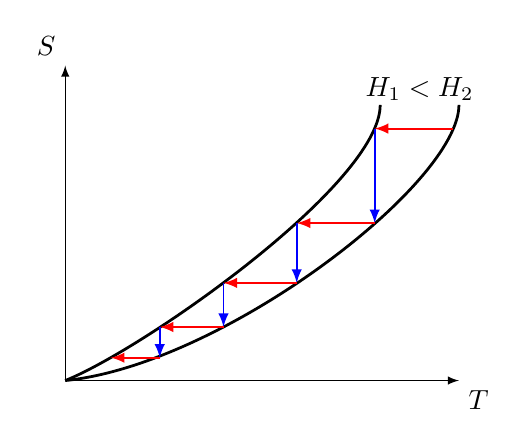
\begin{tikzpicture}
       \draw[-latex] (0,0) -- (5,0) node[below right] {$T$};
       \draw[-latex] (0,0) -- (0,4) node[above left] {$S$};
       \draw[line width=1pt] (0,0) .. controls (1,0.4) and (4,2.5) .. (4,3.5);
       \draw[line width=1pt] (0,0) .. controls (2,0.2) and (5,2.5) .. (5,3.5);
       \draw[-latex,line width=0.7pt,red] (4.92,3.2) -- (3.93,3.2);
       \draw[-latex,line width=0.7pt,blue] (3.93,3.2) -- (3.93,2);
       \draw[-latex,line width=0.7pt,red] (3.93,2) -- (2.94,2);
       \draw[-latex,line width=0.7pt,blue] (2.94,2) -- (2.94,1.24);
       \draw[-latex,line width=0.7pt,red] (2.94,1.24) -- (2.01,1.24);
       \draw[-latex,line width=0.7pt,blue] (2.01,1.24) -- (2.01,0.68);
       \draw[-latex,line width=0.7pt,red] (2.01,0.68) -- (1.2,0.68);
       \draw[-latex,line width=0.7pt,blue] (1.2,0.68) -- (1.2,0.29);
       \draw[-latex,line width=0.7pt,red] (1.2,0.29) -- (0.58,0.29);
       \node at (4.5,3.7) {$H_1 < H_2$};
       \end{tikzpicture}
       \caption{Az adiabatikus lemágnesezés folyamata.
   A piros lépésekben történik az adiabatikus lemágnesezés, a kék lépésekben pedig az izotermikus mágnesezés.}\label{fig:B03-adiablemag}
     \end{figure}
   \end{enumerate}
   

  \chapter{Sokas\'agok, eloszl\'asok, potenci\'alok}
 
 \section{Mikrokanonikus sokaság}
  
  Lásd \aref{ss:B03-mikrokansok}. fejezetet.
  
 \section{Kanonikus sokaság ($T$,$V$,$N$)}
  
  Kanonikus sokaságban egy zárt rendszer kis alrendszerét tekintjük. Az egész rendszer energiája rögzített ($E_0=E+E_\text{K}$), ahol $E$ az alrendszer energiája, míg $E_\text{K}$ a környezeté. Mivel a környezet jóval nagyobb, mint az alrendszer, ezért $E\approx E_\text{K}=\text{áll}$. 
  
  \subsection{A kanonikus eloszlás}
   
   Az eloszlás meghatározásához kiszámoljuk annak a valószínűségét, hogy az alrendszer az $i$-edik mikroállapotban van. Ez a szám azzal lesz egyenlő ahányféleképpen a környezet energiája $E_0-E_i$ lehet:
   \al{
    \rho(i)
     =\frac{\Omega_\text{K}(E_0-E_i,\delta E)}{\Omega_0(E_0,\delta E)}.
   }
   Mivel $E_i$ kicsi, így ezt sorbafejthetjük (a logaritmusát):
   \al{
    \ln\rho(i)
     &=\underbrace{\ln\frac{\Omega_\text{K}(E_0,\delta E)}{\Omega_0(E_0,\delta E)}}_{\text{const.}}-\pder{\ln\Omega_\text{K}(E_0,\delta E)}{E}\cdot E_i+\mathcal{O}(E_i^2)\\
     &=\underbrace{\ln\frac{\Omega_\text{K}(E_0,\delta E)}{\Omega_0(E_0,\delta E)}}_{\text{const.}}-\underbrace{\pder{\ln\Omega_\text{K}(E_\text{K},\delta E)}{E}}_{=\frac{1}{\kB T_\text{K}}}\cdot E_i+\mathcal{O}(E_i^2)
      \approx\text{const.}-\beta_\text{K}E_i.
   }
   Igy $\rho(i)\sim e^{-\beta_\text{K} E_i}$. A normálással együtt klasszikus és kvantumos rendszerre:
   \al{
    &\text{Klasszikus rendszerre:}
    &\rho(q,p)&=\frac{1}{Z}e^{-\beta E(q,p)}
    &Z&=\intl{}{}\frac{\dd q^{dN}\dd p^{dN}}{h^{dN}N!}\,e^{-\beta E(q,p)}\\
    &\text{Kvantumos rendszerre:}
    &\op\rho&=\frac{1}{Z}e^{-\beta \opH}
    &Z&=\tr\left(e^{-\beta \opH}\right),
   }
   ahol megelőlegeztük, hogy a környezet és a rendszer hőmérséklete egyenlő. Ehhez vizsgáljuk meg, hogy mekkora annak a valószínűségi sűrűsége, hogy az általunk vizsgált alrendszer energiája $E$. Ez abból adódik, hogy a rendszer mekkora valószínűséggel van az $i$-edik mikroállapotban, illetve hogy az állapotok milyen sűrűn vannak ($\omega(E)$ az energia-állapotsűrűség): 
   \al{
    P(E)=\rho(E)\omega(E)=\frac{e^{-\beta_\text{K}E}\omega(E)}{Z}.
   }
   Ez egy éles eloszlás, hiszen a számláló első tagja az energia növelésével élesen levág, míg $\omega(E)$ az energia növelésével élesen nő. Az éles eloszlás miatt a várható érték és a legvalószínűbb érték itt is jó közelítéssel megegyezik. Az eloszlás (logaritmusának) maximuma:
   \al{
    \ln P(E)&=-\beta_\text{K}E+\ln\omega(E)+\text{const.}\\
    0&=\pder{\ln P(E)}{E}=-\beta_\text{K}+\underbrace{\pder{\ln \omega(E)}{E}}_{\frac{1}{\kB T}}
    &\Rightarrow
    &&T=T_\text{K}.
   }
  
  \subsection{Energia várható értéke, fluktuációi}
   
   Az energia várható értéke:
   \al{
    \mv{E}
     &=\suml{i}{}E_i\rho(i)
      =\suml{i}{}\frac{E_i e^{-\beta E_i}}{\suml{j}{}e^{-\beta E_j}}
      =-\pder{\ln Z}{\beta},
   }
   illetve szórásnégyzete:
   \al{
    \mv{(\Delta E)^2}
     &=\mv{E^2}-\mv{E}^2
      =\frac{1}{Z}\pder{^2 Z}{\beta^2}-\left(\frac{1}{Z}\pder{Z}{\beta}\right)^2
      =\pder{}{\beta}\left(\frac{1}{Z}\pder{Z}{\beta}\right)
      =\pder{}{\beta}\left(\pder{\ln Z}{\beta}\right)\\
     &=-\pder{E}{\beta}
      =-\kB\underbrace{\pder{E}{T}}_{C_V}\underbrace{\pder{T}{\frac{1}{T}}}_{-T^2}
      =\kB T^2 C_V.
   }
   Az energia szórásnégyzete egy statisztikus fizikai mennyiség, míg a jobb oldalon állók termodinamikai mennyiségek. Mivel feltételeztük, hogy normál rendszerben vagyunk, így $C_V>0$ adódik. A termodinamikában ez stabilitási feltétel.
   
  \subsection{Szabadenergia}
   
   A termodinamikában az energiából Legendre-transzformációval előállítjuk a szabadenergiát: $F=E-TS$. A statisztikus fizikában:
   \al{
    F=-\kB T\ln Z,
   }
   ahol $Z$ az állapotszám. Mivel az eloszlás nagyon éles, ezért az állapotösszeg közelíthető:
   \aln{
    Z=\intl{E_\text{min}}{\infty}\dd E\,e^{-\beta E}\omega(E)
     =e^{-\beta E} \omega(E)\cdot \Delta E,\label{eq:B04-kanallszam}
   }
   ahol $\Delta E$ az eloszlás szélessége. A szórásnégyzetből adódik, hogy $\Delta E\sim C_V\sim N$. Így tehát
   \al{
    F=-\kB T\ln Z
     =-\kB T \big(\underbrace{-\beta E}_{\mathcal{O}(N)} +\underbrace{\ln\omega(E)}_{\mathcal{O}(N)}+ \underbrace{\ln\Delta E}_{\mathcal{O}(\ln N)}\big)
     \approx -\kB T (-\beta E + \ln\omega(E))
     =E-TS,
   }
   vagyis makroszkopikusan megegyezik a termodinamikai definícióval.
   A termodinamikai deriváltaknak megfelelő összefüggéseket is megkapjuk:
   \al{
    \pder{F}{T}
     &=\pder{}{T}(-\kB T \ln Z)
      =-\kB\ln Z-\kB T\pder{\ln Z}{T}
      =\frac{F}{T}+\frac{1}{T}\pder{\ln Z}{\beta}
      =\frac{F}{T}-\frac{E}{T}
      =-S\\
    \pder{F}{V}
     &=\pder{}{V}(-\kB T \ln Z)
      =-\kB T \pder{\ln Z}{V}
      =-\kB T \frac{1}{Z}\suml{i}{}\beta\left(-\pder{E_i}{V}\right)e^{-\beta E_i}
      =\frac{1}{Z}\suml{i}{}\pder{E_i}{V}e^{-\beta E_i}\\
     &=\mv{\pder{E}{V}}=-p
   }
   
   $F$ extenzív mennyiség, hiszen független alrendszerek összességére $Z$ szorzódik. Az információs entrópiába helyettesítve a kanonikus eloszlás az $S$ entrópiát adja:
   \al{
    \kB S_\text{inf}
     &=-\kB\suml{}{}\rho(i)\ln\rho(i)
      =-\kB\frac{1}{Z}\suml{}{}e^{-\beta E_i}\ln\left(\frac{1}{Z}e^{-\beta E_i}\right)\\
     &=-\kB\frac{1}{Z}\suml{}{}e^{-\beta E_i}\left(-\beta E_i-\ln Z \right)
      =\kB\beta\underbrace{\frac{1}{Z}\suml{}{} E_i e^{-\beta E_i}}_{E}
       +\kB\ln Z\underbrace{\frac{1}{Z}\suml{}{}e^{-\beta E_i}}_{1}\\
     &=\frac{E}{T}-\frac{F}{T}
      =S.
   }
   Az információs entrópiát a mikrokanonikus eloszlás maximalizálta. A kanonikus eloszlás az információs entrópiát az a mellékfeltétel mellett maximalizálja, hogy $E$ állandó. Ezt onnan tudjuk, hogy $T$-t rögzíti a környezet, és $T$ az átlagenergia, így fix részecskeszám mellett $E=\suml{}{}E_i\rho(i)=\text{const.}$ A variálás:
   \al{
    0&=\delta\left(-\suml{i}{}\rho(i)\ln\rho(i)-\lambda\suml{i}{}E_i\rho(i)\right)
      =-\suml{i}{}\left(\delta\rho(i)\ln\rho(i)+\rho(i)\frac{1}{\rho(i)}\delta\rho(i)\right)-\lambda\suml{i}{}E_i\delta\rho(i)\\
     &=\suml{i}{}\delta\rho(i)\big(-\ln\rho(i)-1-\lambda E_i\big)\\
    0&=-\ln\rho(i)-1-\lambda E_i\\
    \rho(i)&=C e^{-\lambda E_i},
   }
   ahol $C=Z$ és $\lambda=\beta$. 
   
  \section{Nagykanonikus sokaság ($T$,$V$,$\mu$)}
   
   A konstrukció hasonló az előzőhöz: most is egy elszigetelt nagy rendszer pici alrendszerét vizsgáljuk. Az alrendszer és a környezet között anyagi kölcsönhatás és energiatranszfer történhet, de mechanikai munka nincs ($\delta V=0$). 
   
   Bevezetjük a nagykanonikus potenciált:
   \al{
    \Phi(T,V,N)&=E-TS-\mu N=-pV
    &\dd\Phi=-S\dd T-p\dd V-N\dd\mu
   }
   A termodinamikai deriváltak:
   \al{
    &\left(\pder{\Phi}{T}\right)_{V,\mu}=-S
    &&\left(\pder{\Phi}{V}\right)_{T,\mu}=-p
    &&\left(\pder{\Phi}{\mu}\right)_{T,V}=-N.
   }
   Ebben az esetben egy mikroállapot valószínűsége: $\rho(N,i_N)$. A mikroállapotok valószínűsége attól is függ, hogy hány részecske van épp a rendszerben. Ez felírva a környezet és a teljes rendszer állapotszámaival:
   \al{
    \rho(N,i_N)=\frac{\Omega_{0,\text{K}}(E_0-E,N_0-N)}{\Omega_0(E_0,N_0)}.
   }
   Itt is sorfejtést alkalmazunk a kis $E$ és $N$-re:
   \al{
    \ln\rho(N,i_N)=\text{const}-\pder{\ln\Omega_\text{K}(E_0,N_0)}{E}E_i-\pder{\ln\Omega_\text{K}(E_0,N_0)}{N}N,
   }
   ahonnan exponencializálva és elnevezve az együtthatókat:
   \al{
    &\rho(N,i_N)=\frac{1}{\mathcal{Z}}e^{-\beta_\text{K}(E_i-\mu_\text{K} N)}
    &\mathcal{Z}=\mathcal{Z}(T,V,\mu)=\suml{N=0}{\infty}\suml{i_N}{}e^{-\beta_\text{K}(E_i-\mu_\text{K} N)}
   }
   Itt is a környezet kémiai potenciálja és redukált hőmérséklete szerepel. A kanonikus esethez hasonlóan itt is be lehet látni, hogy a $\beta_\text{K}=\beta$ és $\mu_\text{K}=\mu$.
   
   A nagykanonikus potenciál statisztikus fizikai definíciója:
   \al{
    \Phi=-\kB T\ln\mathcal{Z},
   }
   melyről be lehet látni, hogy az megegyezik a termodinamikai definícióval:
   \al{
    \Phi
     &=-\kB T\ln\mathcal{Z}
      =-\kB T\ln\left(\suml{i}{}e^{-\beta(E_i-\mu N)}\right)
      =-\kB T\ln\left(\suml{N=0}{\infty}e^{\beta\mu N} Z_n\right),
   }
   ahol $Z_N$ a kanonikus állapotszám $N$ részecskére. Használva \eqaref{eq:B04-kanallszam} egyenletet, illetve hogy az eloszlás $N$ szerint is éles
   \al{
    \Phi
     &=-\kB T\ln\left(\suml{N=0}{\infty}e^{\beta\mu N} e^{-\beta E} \omega(E)\cdot \Delta E\right)
      =-\kB T\ln\left(e^{\beta\mu N} e^{-\beta E} \omega(E)\cdot \Delta E\Delta N\right)\\
     &=-\kB T\left(\beta\mu N -\beta E +\ln\omega(E)+\ln\Delta E+\ln\Delta N\right)
      \approx -\mu N + E -\kB T\ln\omega(E)\\
     &=E-TS-\mu N.
   }
   
 \section{TPN sokaság ($T$,$p$,$N$)}
  
  Tekintsünk egy olyan alrendszer, amely mechanikai kapcsolatban van a környezettel és hőátadás is lehetséges. Ennek a termodinamikai potenciálja a szabadentalpia:
  \al{
   &G(T,p,N)=E-TS+pV=\mu N
   &\dd G=-S\dd T+V\dd p+\mu\dd N.
  }
  
  A mikroállapotok valószínűsége:
  \al{
   &\rho(V,i_V)=\frac{1}{Y}e^{-\beta(E_{i_V}+pV)}
   &Y=Y(T,p,N)=\intl{V}{}\drh\suml{i_V}{}e^{-\beta(E_{i_V}+pV)}.
  }
  
  A statisztikus fizikai potenciál definíciója:
  \al{
   G=-\kB T\ln Y,
  }
  amiről szintén meg lehet mutatni, hogy a termodinamikai határesetben megegyezik a szabadentalpiával. A termodinamikai deriváltak:
  \al{
   \pder{G}{T}
    &=-\kB\ln Y-\kB T\pder{\ln Y}{T}
     =\frac{G}{T}+\frac{1}{T}\pder{\ln Y}{\beta}
     =\frac{G}{T}-\frac{E+pV}{T}
     =-S\\
   \pder{G}{p}
    &=-\kB T\pder{\ln Y}{p}
     =\kB T\beta V
     =V\\
   \mv{(\Delta E)^2}
    &=\mv{E^2}-\mv{E}^2
     =\frac{1}{Y}\pder{^2 Y}{\beta^2}-\left(\frac{1}{Y}\pder{Y}{\beta}\right)^2
     =\pder{}{\beta}\left(\frac{1}{Y}\pder{Y}{\beta}\right)
     =\pder{}{\beta}\left(\pder{\ln Y}{\beta}\right)\\
    &=-\pder{E}{\beta}
     =\kB T^2\pder{E}{T}
     =\kB T^2 C_V\\
   \mv{(\Delta V)^2}
    &=\mv{V^2}-\mv{V}^2
     =\frac{1}{Y}\frac{1}{\beta^2}\pder{^2 Y}{p^2}-\left(-\frac{1}{Y}\frac{1}{\beta}\pder{Y}{p}\right)^2
     =\frac{1}{\beta^2}\pder{}{p}\left(\frac{1}{Y}\pder{Y}{p}\right) 
     =\frac{1}{\beta^2}\pder{}{p}\left(\pder{\ln Y}{p}\right) \\
    &=-\kB T\pder{V}{p}
     =\kB T V \kappa_T.
  }
  
  
  
  
  \include{B05tetel/B05tetel}
  \chapter{Klasszikus g\'azok: ide\'alis g\'az, ekvipart\'{\i}ci\'o, Maxwell-eloszl\'as, viri\'al sorfejt\'es, van der Waals \'allapotegyenlet} 
 
 \section{Ekvipartíció tétele}
  
  Tekintsünk egy klasszikus rendszert. Ennek Hamilton-függvénye $H=H(q,p)$. Jelölje $x_i$ a Hamilton-függvény tetszőleges változóját, $q_i$-t vagy akár $p_i$-t is. Az $x_i$-t szabadsági foknak hívjuk, ha 
  \al{
   \lim_{x_i\to \pm\infty}H(\dots,x_i,\dots)=\infty.
  }
  Fontos, hogy mind a két határértékben divergálnia kell a Hamilton-függvénynek. Az ekvipartíció tétele kimondja, hogy ha $x_i$ szabadsági fok, akkor 
  \al{
   \mv{x_j\pder{H}{x_i}}=\delta_{ij}\kB T.
  }
  Bizonyítás:
  \al{
   \mv{x_j\pder{H}{x_i}}
    &=\frac{1}{Z}\intl{}{}\frac{\dd^{dN}p\dd^{dN}q}{N! h^{dN}}\,e^{-\beta H}x_j\pder{H}{x_i},
  }
  ahol végezzük el külön az $x_i$-re való integráli:
  \al{
   \intl{}{}\dd x_i\,e^{-\beta H}x_j\pder{H}{x_i}
    &=-\frac{1}{\beta}\intl{}{}\dd x_i\,x_j\pder{e^{-\beta H}}{x_i}
     =\{\text{parc. int.}\}\\
    &=-\frac{1}{\beta}\left(\left[x_j e^{-\beta H}\right]_{x_i=-\infty}^{x_i=\infty}-\intl{}{}\dd x_i\,\pder{x_j}{x_i}e^{-\beta H}\right)
     =\frac{1}{\beta}\intl{}{}\dd x_i\,\underbrace{\pder{x_j}{x_i}}_{\delta_{ij}} e^{-\beta H},
  } 
  így
  \al{
   \mv{x_j\pder{H}{x_i}}
    &=\frac{1}{Z}\frac{1}{N! h^{dN}}\intl{}{}\dd^{dN}p\dd^{dN}q\,\frac{1}{\beta}\pder{x_j}{x_i}e^{-\beta H}
     =\frac{1}{\beta}\delta_{ij}\frac{1}{Z}\underbrace{\frac{1}{N! h^{dN}}\intl{}{}\dd^{dN}p\dd^{dN}q\,e^{-\beta H}}_{=Z}
     =\kB T\delta_{ij}.
  }
  
  Még egyszer, ez csak klasszikus rendszerekben igaz. Alacsony hőmérsékleten nem ugyanakkora energia jut az egyes szabadsági fokokra, vannak szabadsági fokok, amelyek kifagynak. Pl. a Doulong--Petit-törvény szerint a harmonikus oszcillátor fajhője állandó, míg a kvantumos levezetésből alacsony hőmérsékleten $\sim T^2$ adódik. 
  
 \section{Klasszikus ideális gáz}\label{ss:B06-CID}
  
  Ideális klasszikus gáznak tekintjük azt a rendszert, amely
  \begin{itemize}
   \item klasszikus (nem kvantumos) fizikával leírható,
   \item a részecskék pontszerűnek tekinthetőek (térfogatuk elhanyagolható),
   \item a falakkal tökéletesen rugalmasan ütköznek a részecskék (energia megmarad),
   \item a részecskék közötti kölcsönhatást csak olyan értelemben vesszük figyelembe, hogy a rendszer termalizálódik, egyéb effektusokkal nem számolunk.
  \end{itemize}
  
  \subsection{Állapotszám}
  
   Legyen $N$ részecske a $d$ dimenziós, $V$ térfogatot kitöltő klasszikus ideális gázban. Mikrokanonikus sokaságként kezelve az állapotszám:
   \al{
    \Omega_{0}(E)
     =\intl{\suml{i=1}{N}\frac{p_i^2}{2m}<E}{}\frac{\dd^{dN}p\dd^{dN}q}{N! h^{dN}}\,
     =\frac{V^{N}}{N! h^{dN}}\underbrace{\intl{p_1^2+p_2^2+\dots<2mE}{}\,\dd^{dN}p}_{\substack{\text{$dN$ dimenziós $\sqrt{2mE}$}\\ \text{sugarú gömb térfogata}}}
     =\frac{V^{N}}{N! h^{dN}}\frac{(2mE)^{\frac{dN}{2}}\pi^{\frac{dN}{2}}}{\Gamma\left(\frac{dN}{2}+1\right)},
   }
   ahol $\Gamma$ a Gamma-függvény (a faktoriális általánosítása).
   
   Az entrópiához szükségünk van ennek a logaritmusára. A Stirling-formulát ($\ln n!\approx n\ln n-n$) használva, illetve a Gamma-függvényt közelítve ($\Gamma(n+1)\sim n!$): 
   \al{
    \ln{\Omega_0(E)}
     &\approx N\ln V-(N\ln N-N)-dN\ln h+\frac{dN}{2}\ln(2mE\pi)-\left(\frac{dN}{2}\ln\frac{dN}{2}-\frac{dN}{2}\right)+\mathcal{O}(\ln N)\\
     &=N\ln V-(N\ln N-N)+\frac{dN}{2}\ln\left(\frac{4mE\pi}{dNh^2}\right)+\frac{dN}{2}+\mathcal{O}(\ln N)\\
     &=\frac{2+d}{2}N+\frac{dN}{2}\ln\left(\frac{4m\pi}{dh^2}\frac{E}{N}\left(\frac{V}{N}\right)^{\frac{2}{d}}\right)+\mathcal{O}(\ln N)\\
     &=N\underbrace{\left[\frac{2+d}{2}+\frac{d}{2}\ln\left(\frac{4m\pi}{dh^2}\frac{E}{N}\left(\frac{V}{N}\right)^{\frac{2}{d}}\right)\right]}_{=\phi\left(\frac{E}{N},\frac{V}{N}\right)}+\mathcal{O}(\ln N).
   }
   Láthatjuk, hogy ez egy normál rendszer \eqaref{eq:B03-Omega--N} egyenlet alapján. 
   
  \subsection{Maxwell-féle sebességeloszlás}
   
   Írjuk le az ideális gázt kanonikus sokaságban. A Hamilton-függvény $H=\suml{i=1}{N}\frac{p_i^2}{2m}$. Mivel a Hamilton kölcsönhatásmentes, így a kanonikus állapotszám:
   \al{
    Z&=\frac{Z_1^N}{N!}\\
    Z_1&=\frac{1}{h^3}\intl{}{}\dd^3 \qv\dd^3 \pv\,e^{-\beta\frac{p^2}{2m}}
        =\frac{V}{h^3}\intl{}{}\dd^3 \pv\,e^{-\beta\frac{\pv^2}{2m}}
       =\frac{V}{h^3}\left(\frac{2m\pi}{\beta}\right)^{\frac{3}{2}}
        =\frac{V}{h^3}\left(2\pi m\kB T\right)^{\frac{3}{2}}.
   }
   Annak a valószínűsége, hogy egy részecske impulzusa $\pv$:
   \al{
    P(\pv)
     =\frac{\frac{1}{h^{3N}}\intl{}{}\dd^{3N} q\dd^{3(N-1)} p\,e^{-\beta\suml{i=1}{N}\frac{p_i^2}{2m}}}{Z}
     =\frac{\frac{V}{h^3}e^{-\beta\frac{\pv^2}{2m}}}{Z_1}
     =\frac{e^{-\beta\frac{\pv^2}{2m}}}{\left(2\pi m\kB T\right)^{\frac{3}{2}}}.
   }
   Az előző állítás nem csak kölcsönhatásmentes rendszerekre igaz, hanem olyanokra is, ahol a kölcsönhatás csak a $q$-tól függ. Az előző képletben a számlálóban és a nevezőben ugyanaz a térintegrál lenne, így egyszerűsíteni lehetne vele.
   
   Az impulzus eloszlásából kifejezhetjük, hogy mennyi a valószínűsége, hogy a részecske sebessége $\vv$, hiszen:
   \al{
    &P(\vv)\dd^3\vv=P(\pv)\dd^3\pv
    &\pv=m\vv
    &&P(\vv)=m^3 P(\pv)=\left(\frac{m}{2\pi \kB T}\right)^{\frac{3}{2}}e^{-\frac{m\vv^2}{2\kB T}}.
   }
   A sebesség abszolút értékének eloszlása a Maxwell-féle sebességeloszlás:
   \al{
    &\dd^3\vv=4\pi v^2\dd v
    &P(v)
     =4\pi v^2 P(\vv)
   }
   \aln{
     \boxed{P(v)=4\pi v^2\left(\frac{m}{2\pi \kB T}\right)^{\frac{3}{2}}e^{-\frac{m v^2}{2\kB T}}}.\label{eq:B06-Maxwell}
   }
   
   Az eloszlás maximumhelye:
   \al{
    P'(v)
     &=0
      =\der{}{v}\left(-\frac{m v^2}{2\kB T}+2\ln v\right)
      =-\frac{m v}{\kB T}+2\frac{1}{v}
     &v_\text{max}=\sqrt{\frac{2\kB T}{m}},
   }
   várható értéke és négyzetes közepe:
   \al{
    \mv{v}
     &=\intl{0}{\infty}\dd v\, vP(v)
      =\intl{0}{\infty}\dd v\, 4\pi v^3\left(\frac{m}{2\pi \kB T}\right)^{\frac{3}{2}}e^{-\frac{m v^2}{2\kB T}}
      =\sqrt{\frac{8\kB T}{\pi m}}\\
    \mv{v^2}
     &=\frac{2}{m}\frac{3}{2}\kB T
      =\frac{3\kB T}{m}.
   }
   Itt messze nem igaz, hogy az eloszlás éles lenne, egy részecske sebességének az eloszlása igen széles tartományban van. 
   
   Az energia szerinti eloszláshoz:
   \al{
    &\dd E=mv\dd v
    &E=\frac{1}{2}mv^2
    &&P(E)=\frac{1}{mv}P(v)
   }
   \al{
    P(E)
     &=\frac{1}{m}4\pi v\left(\frac{m}{2\pi \kB T}\right)^{\frac{3}{2}}e^{-\frac{m v^2}{2\kB T}}
      =\frac{1}{m}4\pi \sqrt{\frac{2E}{m}}\left(\frac{m}{2\pi \kB T}\right)^{\frac{3}{2}}e^{-\frac{E}{\kB T}}
      =2\pi \sqrt{E}\left(\frac{1}{\pi \kB T}\right)^{\frac{3}{2}}e^{-\frac{E}{\kB T}}.
   }
   Ennek maximumhelye és várható értéke:
   \al{
    \der{}{E}P(E)&=0
      =\der{}{E}\left(-\frac{E}{\kB T}+\frac{1}{2}\ln E\right)
      =-\frac{1}{\kB T}+\frac{1}{2E}
     & E_\text{max}=\frac{1}{2}\kB T\\
    \mv{E}&=\frac{3}{2}\kB T.
   }
   
   Az energia szórása:
   \al{
    \mv{(\Delta E)^2}
     &=\mv{E^2}-\mv{E}^2
      =\pder{}{\beta}\pder{\ln Z_1}{\beta}
      =\frac{3}{2}(\kB T)^2
      =\frac{2}{3}\mv{E}^2\\
     \frac{\sqrt{\mv{(\Delta E)^2}}}{\mv{E}}
      &=\sqrt{\frac{2}{3}}\sim\mathcal{O}(1),
   }
   ami egy részecskére igen jelentős, de az $N$ részecskéből álló gázra, ahol
   \al{
    \ln Z
     &=\ln\left(\frac{Z_1^N}{N!}\right)
      \approx -N\ln N+N+N\ln Z_1
      =-N\ln N+N+N\ln \left(\frac{V}{h^3}\left(2\pi m\kB T\right)^{\frac{3}{2}}\right)\\
    \mv{(\Delta E)^2}
     &=\pder{}{\beta}\pder{\ln Z}{\beta}
      \sim N\\
    \frac{\sqrt{\mv{(\Delta E)^2}}}{\mv{E}}&\sim\frac{1}{\sqrt{N}}.
   }
   
   Az ideális gáz állapotegyenletét megadhatjuk pl.\ az $F$ termodinamikai deriváltjával:
   \al{
    p&=-\pder{F}{V}
      =-\pder{}{V}\left(-\kB T \ln Z\right)
      =-\pder{}{V}\left(-\kB T N\ln \left(\frac{V}{N h^3}\left(2\pi m\kB T\right)^{\frac{3}{2}}\right)\right)\\
     &=\frac{1}{V}\kB T N\\
    pV&=N\kB T.
   }
   
 \section{Viriál tétel}
  
  Tegyük fel, hogy a klasszikus háromdimenziós rendszerünk Hamilton-függvénye a következő:
  \al{
   H=E_\text{kin}+U_\text{pot}=E_\text{kin}+U_\text{int}+U_\text{w},
  }
  ahol a kölcsönhatást két részre osztottuk, a részecskék egymással való kölcsönhatására és a fallal való kölcsönhatásra. Azt tudjuk az ekvipartíció tétele miatt, hogy $\mv{E_\text{kin}}=\frac{3}{2}\kB T$. Kérdés, hogy mennyi a potenciális energia átlagértéke. 
  
  A Newton-egyenletből:
  \al{
   m_i \ddot{x}_i=F_i=-\pder{U_\text{pot}}{x_i}=-\pder{H}{x_i}.
  }
  Ez beszorozva $x_i$-vel és kicsit átalakítva:
  \al{
   \der{}{t}\left(\frac{1}{2}m_ix_i\dot{x}_i\right)-\frac{1}{2}m_i\dot{x}_i^2=\underbrace{\frac{1}{2}x_i F_i}_{\text{viriál}}.
  }
  Az egyenlet időátlaga:
  \al{
   \underbrace{\lim_{\tau\to\infty}\frac{1}{\tau}\intl{0}{\tau}\dd t\,
   \der{}{t}\left(\frac{1}{2}m_ix_i\dot{x}_i\right)}_{\text{I.}}
   -\underbrace{\lim_{\tau\to\infty}\frac{1}{\tau}\intl{0}{\tau}\dd t\,\frac{1}{2}m_i\dot{x}_i^2}_{\text{II.}}
   &=\underbrace{\lim_{\tau\to\infty}\frac{1}{\tau}\intl{0}{\tau}\dd t\,\frac{1}{2}x_i F_i}_{\text{III.}}
  }
  A tagok kifejtve:
  \al{
   \text{I.}
    &=\lim_{\tau\to\infty}\frac{1}{\tau}\underbrace{\left[\frac{1}{2}m_ix_i\dot{x}_i\right]_{0}^{\tau}}_{\text{véges}}=0\\
   \text{II.}
    &=\lim_{\tau\to\infty}\frac{1}{\tau}\intl{0}{\tau}\dd t\,\frac{1}{2}m_i\dot{x}_i^2
     =\mv{E_{\text{kin},i}}\\
   \text{III.}
    &=\lim_{\tau\to\infty}\frac{1}{\tau}\intl{0}{\tau}\dd t\,\frac{1}{2}x_i F_i
     =\frac{1}{2}\mv{x_i F_i},
  }
  ahonnan a viriál tétel $i$-re való összegzéssel:
  \aln{
   \boxed{0=\mv{E_\text{kin}}+\frac{1}{2}\mv{\suml{i=1}{3N}x_i F_i}}.\label{eq:B06-virialtetel}
  }
  
  Először tekintsük csak a fallal való kölcsönhatást. 
  \al{
   U_\text{w}=\suml{i=1}{N}\ointl{\partial V}{}\dd A_\rv w(\rv_i-\rv),
  }
  ahol az integrál a fal teljes felületére megy. Ezzel a viriál átlagértéke:
  \al{
   \frac{1}{2}\mv{\suml{i=1}{3N}x_i F_i}
    &=-\frac{1}{2}\mv{\suml{i=1}{N}\rv_i\pder{U_\text{w}}{\rv_i}}
     =-\frac{1}{2}\mv{\suml{i=1}{N}\rv_i\ointl{\partial V}{}\dd A_\rv \grad_i w(\rv_i-\rv)}\\
    &=-\frac{1}{2}\mv{\suml{i=1}{N}\ointl{\partial V}{}\dd A_\rv \rv_i\underbrace{\grad_i w(\rv_i-\rv)}_{\text{nagyon éles}}}
     =-\frac{1}{2}\mv{\suml{i=1}{N}\ointl{\partial V}{}\dd A_\rv \rv\grad_i w(\rv_i-\rv)}\\
    &=\frac{1}{2}\mv{\suml{i=1}{N}\ointl{\partial V}{}\dd A_\rv \rv\grad_\rv w(\rv_i-\rv)}
     =\frac{1}{2}\ointl{\partial V}{}\dd A_\rv \rv\underbrace{\grad_\rv\mv{\suml{i=1}{N} w(\rv_i-\rv)}}_{\substack{\text{erő felületi sűrűsége,}\\\text{azaz a nyomás}}}\\
    &=\frac{1}{2}\ointl{\partial V}{}\dd A_\rv \rv \left(-\ev_\text{felület} p\right)
     =-\frac{p}{2}\ointl{\partial V}{}\df_\rv \rv
     =-\frac{p}{2}\intl{V}{}\drh \divo\rv
     =-\frac{3}{2}p\intl{V}{}\drh
     =-\frac{3}{2}pV.
  }
  Összefoglalva a viriál tétel:
  \al{
   \mv{E_\text{kin}}=\frac{3}{2}pV
  }
  
 \section{Viriál sorfejtés}
  
  Most vesszük figyelembe a gáz részecskéi közötti párkölcsönhatásokat:
  \al{
   U_\text{int}
    &=\suml{\mv{i,j}}{}U(\rv_i-\rv_j)
  }A viriál tétel alapján:
  \al{
   pV
    &=\frac{2}{3}\mv{E_\text{kin}}+\frac{2}{3}\frac{1}{2}\mv{\suml{i=1}{N}\rv_i\Fv_i}
     =\frac{2}{3}\mv{E_\text{kin}}-\frac{2}{3}\frac{1}{2}\mv{\suml{i=1}{N}\rv_i\suml{j(\ne i)}{}\pder{U(\rv_i-\rv_j)}{\rv_i}}\\
    &=\frac{2}{3}\mv{E_\text{kin}}-\frac{2}{3}\frac{1}{2}\frac{1}{2}\mv{\suml{i}{}\suml{j(\ne i)}{}\left(\rv_i\pder{U(\rv_i-\rv_j)}{\rv_i}+\rv_j\pder{U(\rv_i-\rv_j)}{\rv_j}\right)}\\
    &=\frac{2}{3}\mv{E_\text{kin}}-\frac{1}{6}\mv{\suml{i\ne j}{N}(\rv_i-\rv_j)\pder{U(\rv)}{\rv}}.
  }
  A jobb oldal a sorba fejthető: $p=n\kB T\big[1+b(T)n+c(T)n^2+\dots\big]$, ahol $b(T)$, $c(T)$\dots a viriál együtthatók.
  
  \subsection{Klasszikus híg gázok viriál sorfejtése}
   
   Nagykanonikus sokasággal felírva:
   \aln{
    pV=-\Phi=\kB T\ln\mathcal{Z}
     =\kB T\ln\left(\suml{N=0}{\infty}Z_Ne^{\beta\mu N}\right).\label{eq:B06-virialsf1}
   }
   Ideális gázra Láttuk, hogy 
   \al{
    &Z_1=\frac{V}{h^3}\left(2\pi m\kB T\right)^{\frac{3}{2}}
     =\frac{V}{\lambda_T^3}
    &\lambda_T=\frac{h}{\sqrt{2m\pi\kB T}},
   }
   így az állapotegyenlet
   \al{
    pV&=\kB T\ln\left(\suml{N=0}{\infty}\frac{1}{N!}(Z_1 e^{\beta\mu })^N\right)
     =\kB T Z_1 e^{\beta\mu}
     =\kB T \frac{V}{\lambda_T^3} e^{\beta\mu}
     =N\kB T,
   }
   ahonnan $e^{\beta\mu}=\lambda_T^3 n$. $\lambda_T$ értéke fix és pici, így ha $n$ kicsi, akkor $e^{\beta\mu}$ is az. Nem ideális gázra is azt gondoljuk, hogy ez kicsi marad, így ez a kis paraméter, ami szerint \eqaref{eq:B06-virialsf1} egyenlet jobb oldalát sorba fejtjük. Az állapotösszeg: $\mathcal{Z}=1+Z_1 e^{\beta\mu}+Z_2 e^{2\beta\mu}+\dots$, illetve $\ln(1+x)=x-\frac{x^2}{2}+\dots$, így
   \al{
    pV&=\kB T\ln\left(1+Z_1 e^{\beta\mu}+Z_2 e^{2\beta\mu}+\dots\right)\\
      &=\kB T\Big(Z_1 e^{\beta\mu}+Z_2 e^{2\beta\mu}+\dots-\frac{1}{2}\left(Z_1 e^{\beta\mu}+Z_2 e^{2\beta\mu}+\dots\right)^2+\dots\Big)\\
      &=\kB T\bigg(\underbrace{Z_1}_{z_1} e^{\beta\mu}+\underbrace{\left(Z_2-\frac{1}{2}Z_1^2\right)}_{z_2} e^{2\beta\mu}+\dots\bigg).
   }
   A részecskeszámot szeretnénk inkább látni az egyenlet jobb oldalán, így kifejezzük azt is
   \al{
    N=\pder{\ln\mathcal{Z}}{(\beta\mu)}
     =z_1 e^{\beta\mu}+2z_2 e^{2\beta\mu}+\dots.
   }
   Itt kicsi hibát vétünk, ha felhasználjuk az ideális gáznál kapott $e^{\mu\beta}=\frac{N}{z_1}$ összefüggést a másodrendű tagban:
   \al{
    N
     &=z_1 e^{\beta\mu}+2 z_2 \frac{N^2}{z_1^2}+\dots,
     &\Rightarrow
     &&z_1 e^{\beta\mu}\approx N-2 z_2 \frac{N^2}{z_1^2}.
   }
   Ezeket behelyettesítve a sorfejtésbe:
   \al{
    pV
     &\approx \kB T\left(z_1 e^{\mu\beta}+z_2 e^{2\mu\beta}\right)
      =\kB T\left(N-2 z_2 \frac{N^2}{z_1^2}+z_2 \frac{N^2}{z_1^2}\right)
      =\kB T\left(N-z_2 \frac{N^2}{z_1^2}\right)\\
     &=N\kB T\left(1-N\frac{Z_2-\frac{1}{2}Z_1^2}{Z_1^2}\right).
   }
   Már csak $Z_1$-et és $Z_2$-t kell kiszámolni. $Z_1$ az egyrészecskés állapotösszeg, ebben nem szerepel kölcsönhatás, így ezt ismerjük. A kétrészecskés állapotösszeg definíció szerint:
   \al{
    Z_2
     &=\intl{}{}\frac{\dd^3\pv_1\dd^3\pv_2\dd^3\rv_1\dd^3\rv_2}{2 h^6}\,e^{-\beta\big(\frac{\pv_1^2}{2m}+\frac{\pv_2^2}{2m}+U(\rv_1-\rv_2)\big)}
      =\frac{1}{2\lambda_T^6}\intl{}{}\dd^3\rv_1\dd^3\rv_2\,e^{-\beta U(\rv_1-\rv_2)}\\
     &=\frac{V}{2\lambda_T^6}\intl{}{}\dd^3\rv\,e^{-\beta U(\rv)}.
   }
   Mellyek a $b(T)$ viriál együttható:
   \al{
    b(T)
     &=-V\frac{Z_2-\frac{1}{2}Z_1^2}{Z_1^2}
      =-\frac{V}{2}\left(\frac{2 Z_2}{Z_1^2}-1\right)
      =-\frac{V}{2}\left(\frac{2 \lambda_T^6 Z_2}{V^2}-1\right)\\
     &=-\frac{V}{2}\left(\frac{2 \lambda_T^6}{V^2}\frac{V}{2\lambda_T^6}\intl{}{}\dd^3\rv\,e^{-\beta U(\rv)}-1\right)
      =-\frac{1}{2}\left(\intl{}{}\dd^3\rv\,e^{-\beta U(\rv)}-V\right)\\
     &=-\frac{1}{2}\intl{}{}\dd^3\rv\,\left(e^{-\beta U(\rv)}-1\right)
   }
   
   \paragraph{Példa: híg gáz, kemény mag}
    
    Legyen a kölcsönhatás ``hard ball'' potenciál:
    \al{
     U_\text{int}=\begin{cases}
                   \infty, & \text{ha }r<\sigma\\
                   0, & \text{ha }r>\sigma.
                  \end{cases}
    }
    Erre:
    \al{
     b(T)
     &=-\frac{1}{2}\intl{0}{\infty}\dd^3\rv\,\left(e^{-\beta U(\rv)}-1\right)
      =-\frac{1}{2}\intl{0}{\infty}\dd r\,4\pi r^2\left(e^{-\beta U(r)}-1\right)
      =\frac{1}{2}\intl{0}{\sigma}\dd r\,4\pi r^2
      =\frac{2\pi}{3}\sigma^3,
    }
    mellyel:
    \al{
     pV=N\kB T\left[1+\frac{N}{V}\frac{2\pi}{3}\sigma^3+\dots\right].
    }
    A nyomás tehát megnő, ami annak köszönhető, hogy a részecskék kicsit taszítják egymást. 
    
 \section{van der Waals állapotegyenlet}
  
  Célunk, hogy leírjuk a folyadák--gáz fázisátalakulást. A viriál sorfejtéssel kapott állapotegyenlet azonban nem lesz kielégítő semmilyen fázisátalakulás közelében, hiszen ott nemanalitikus viselkedést mutatnak a termodinamikai mennyiségek, amely sorfejtésből nem származtatható.
  
  A továbbiak \aref{ss:B09-vdW}. fejezetben.
  \chapter{Kvantumg\'azok: ide\'alis kvantumg\'azok, klasszikus hat\'areset, Fermi- \'es Bose-g\'azok alacsony h\H{o}m\'ers\'ekleten}
 
 \section{Ideális kvantumgázok}
  
  Ideális kvantumgáznak nevezzük azt az $N$ részecskéből álló rendszert, ha annak Hamilton-operátorát a
  \al{
   \opH=\suml{i=1}{dN}\opH_i
  }
  egyrészecske Hamilton-operátorok összegeként fel lehet írni. Klasszikus esetben $\opH_i=\frac{\opp_i^2}{2m}$. Tekintsük ezt a gázt egy $V$ térfogatú dobozban. A hullámfüggvényeket úgy választjuk, hogy azok eltűnjenek a dogoz falán. Ekkor az energia $\ep(k_i)=\frac{\hbar^2 k_i^2}{2m}$, ahol $k_i=\frac{\pi}{L}n_i$ $n_i\in\mathbb{N}^+$ minden $i$-re.
  
  \subsection{Állapotszám}
  
   A rendszer egy mikroállapotát egy $\alpha=\{n_1, n_2,\dots,n_{dN}\}$ számsorozat jellemzi. Az állapotszám:
   \al{
    \Omega_0(E)
     &=\suml{E_v}{}\Theta\left(E-E_\alpha\right)
      =\suml{\alpha}{}\Theta\left(E-\frac{\hbar^2 }{2m}\frac{\pi^2}{L^2}n_\alpha^2\right)
      =\suml{\alpha}{}\Theta\left(\frac{2mE L^2}{\hbar^2\pi^2}-n_\alpha^2\right).
   }
   Ha elég sűrűn helyezkednek el az állapotok, akkor ez éppen egy $dN$ dimenziós gömb ``pozitív'' $\left(\frac{1}{2}\right)^{dN}$-ed részének a térfogata. Mivel a részecskék nem megkülönböztethetőek, ezért:
   \al{
    \Omega_0(E)=\frac{1}{N!}\cdot \frac{\pi^{\frac{dN}{2}}}{\Gamma\left({\frac{dN}{2}}+1\right)}\left(\frac{2mE L^2}{\hbar^2\pi^2}\right)^{\frac{dN}{2}}\left(\frac{1}{2}\right)^{dN}.
   } 
   Ez megegyezik a klasszikus esettel a $V=L^d$ helyettesítéssel.
   
  \subsection{Hullámfüggvények}
   
   Az egyrészecske Hamilton-operátorok megoldásai az egyrészecske hullámfüggvények: 
   \al{
    \opH_i\varphi_{m_i}(r_i,\sigma_i)=\ep_{m,i}\varphi_{m_i}(r_i,\sigma_i).
   }
   Ebből a teljes rendszer hullámfüggvényét szorzat alakban tudjuk előállítani:
   \al{
    \Psi_{m_1,\dots,m_{dN}}\big(r_1,\sigma_1;\dots;r_{dN},\sigma_{dN}\big)
     &=\prodl{i=1}{dN}\varphi_{m_i}(r_i,\sigma_i)\\
    \opH\Psi_{m_1,\dots,m_{dN}}\big(r_1,\sigma_1;\dots;r_{dN},\sigma_{dN}\big)
     &=\bigg(\suml{i=1}{N}\ep_{m_i}\bigg)\Psi_{m_1,\dots,m_{dN}}\big(r_1,\sigma_1;\dots;r_{dN},\sigma_{dN}\big)
   }
   Fontos azonban, hogy a részecskék nem megkülönböztethetőek. Ennek következménye, hogy két részecske cseréjére minden mérhető fizikai mennyiségnek változatlannak kell lennie. Legalább két dimenzióban a részecskecsere elvégezhető forgatással. Így belátható, hogy ha a rendszer spinje félegész akkor a hullámfüggvény előjelet vált a részecskecserére, ha pedig egész, akkor nem vált előjelet. Az előzőt fermionikus, az utóbbit bozonikus rendszernek hívjuk. 
   
   Hogy ezt a hullámfüggvények is tükrözzék, fermionikus rendszerben teljesen antiszimmetrizálni kell a hullámfüggvényt:
   \al{
    &\Psi^\text{F}_{m_1,\dots,m_{dN}}\big(r_1,\sigma_1;\dots;r_{dN},\sigma_{dN}\big)\\
     &\qquad\qquad=\frac{1}{\sqrt{N!}}\suml{p\in S_n}{}(-1)^{\pi(p)}\prodl{i=1}{dN}\varphi_{m_i}(r_{p(i)},\sigma_{p(i)})\\
     &\qquad\qquad=\frac{1}{\sqrt{N!}}\suml{p\in S_n}{}(-1)^{\pi(p)}\varphi_{m_1}(r_{p(1)},\sigma_{p(1)})\cdot\varphi_{m_2}(r_{p(2)},\sigma_{p(2)})\cdots\varphi_{m_{dN}}(r_{p(dN)},\sigma_{p(dN)}).
   }
   Itt a $p$ egy permutáció, $\pi(p)$ a permutáció paritása. Az $\frac{1}{\sqrt{N!}}$ faktor a normálás miatt szükséges.
   
   Bozonikus rendszerre a hullámfüggvényt szimmetrizáljuk:
   \al{
    \Psi^\text{B}_{m_1,\dots,m_{dN}}\big(r_1,\sigma_1;\dots;r_{dN},\sigma_{dN}\big)
     =\sqrt{\frac{n_1!n_2!\cdots n_{dN}!}{N!}}\suml{p\in S_n}{}\prodl{i=1}{dN}\varphi_{m_i}(r_{p(i)},\sigma_{p(i)}),
   }
   ahol csak azokra az állapotokra összegzünk, ahol a betöltési számok különbözőek. A betöltési számok ($n_m$)-k azt adják meg, hogy hány részecske található az $\varphi_m$ állapotban. Ez egy számsorozat, aminek ismeretében a hullámfüggvényeket meg lehet konstruálni. Fermionikus rendszerre $n_m=\{0,1\}$, bozonikusra $n_m=\{0,1,2,\dots\}$. A betöltési számokkal felírható a rendszer teljes energiája: $E=\suml{m=1}{\infty}n_m\ep_m$, ahol az összegzés az egyrészecske állapotokra történik.
   
  \subsection{Betöltési számok}
  
   Nagykanonikus sokaságot használva:
   \al{
    \mathcal{Z}
     &=\suml{N=0}{\infty}e^{\beta\mu N}\suml{\substack{\{n_m\}\\ \suml{m}{}n_m=N}}{}e^{-\beta E(\{n_m\})}
      =\suml{\{n_m\}}{}e^{\beta\mu N(\{n_m\})}\cdot e^{-\beta E(\{n_m\})}\\
     &=\suml{\{n_m\}}{}e^{-\beta \suml{m=1}{\infty}n_m\ep_m}\cdot e^{\beta\mu \suml{m=1}{\infty}n_m}
      =\suml{\{n_m\}}{}e^{-\beta \suml{m=1}{\infty}n_m(\ep_m-\mu)}
      =\suml{\{n_m\}}{}\prodl{m=1}{\infty}e^{-\beta n_m(\ep_m-\mu)}.
   }
   Itt megcseréljük a szummát és a produktumot. Eddig azt történt, hogy fixáltunk egy betöltési szám konfigurációt, és végigmentünk minden egyrészecske állapoton, és annyiszor vettük figyelembe a hozzá tartozó súlyt, ahány részecske volt abban az állapotban. Most úgy fogunk összegezni, hogy végigmegyünk egyesével az összes egyrészecske állapoton, és mindegyik állapotban sorra vesszük az összes lehetséges betöltés súlyát:
   \al{
    \mathcal{Z}
     &=\prodl{m}{}\underbrace{\suml{n=0}{n_\text{max}}e^{-\beta n(\ep_m-\mu)}}_{\mathcal{Z}^{F/B}_m}.
   }
   Az $n_\text{max}$ attól függ, hogy milyen típusúak a részecskéink. Fermionokra, illetve bozonokra:
   \al{
    \mathcal{Z}^{F}_m
     &=\suml{n=0}{n_\text{max}=1}e^{-\beta n(\ep_m-\mu)}
     =1+e^{-\beta (\ep_m-\mu)}\\
    \mathcal{Z}^{B}_m
     &=\suml{n=0}{n_\text{max}=\infty}e^{-\beta n(\ep_m-\mu)}
      =\frac{1}{1-e^{-\beta (\ep_m-\mu)}}.
   }
   A bozonoknál a geometriai sor felösszegzésének feltétele, hogy $\ep_m>\mu$ minden $m$-re, vagyis hogy $\ep_0=0>\mu$ igaz legyen.
   
   Innen a nagykanonikus állapotszám, potenciál, és a betöltési számok várható értéke:
   \al{
    \mathcal{Z^{F/B}}
     &=\prodl{m}{}\begin{cases}
                   \displaystyle 1+e^{-\beta (\ep_m-\mu)}\\
                  \displaystyle\frac{1}{1-e^{-\beta (\ep_m-\mu)}}
                  \end{cases}&
    \Phi^{F/B}
     &=-\kB T\ln\mathcal{Z^{F/B}}
      =\mp\kB T\suml{m}{}\ln\big(1\pm e^{-\beta (\ep_m-\mu)}\big)
   }
   \al{
    \mv{n_k^{F/B}}
     &=\frac{ 
             \prodl{m}{}\suml{n=0}{n_\text{max}^{F/B}} n_k e^{-\beta n(\ep_m-\mu)}
            }{
             \prodl{m}{}\suml{n=0}{n_\text{max}^{F/B}} e^{-\beta n(\ep_m-\mu)}
            }
      =\frac{\suml{n=0}{n_\text{max}^{F/B}} n e^{-\beta n(\ep_k-\mu)}}{\suml{n=0}{n_\text{max}^{F/B}} e^{-\beta n(\ep_k-\mu)}}
      =\pder{\ln\mathcal{Z}^{F/B}_k}{\beta\mu}\\
     &=\begin{cases}
        \displaystyle\frac{e^{-\beta (\ep_k-\mu)}}{1+e^{-\beta (\ep_k-\mu)}}\\
        \displaystyle\frac{-\frac{-e^{\beta (\ep_k-\mu)}}{\left(1-e^{-\beta (\ep_k-\mu)}\right)^2}}{\frac{1}{1-e^{-\beta (\ep_k-\mu)}}}
       \end{cases}
      =\frac{1}{e^{\beta(\ep_k-\mu)}\pm 1}.
   }
   Ennek ismeretében a nagykanonikus potenciál, a várható részecskeszám és energia:
   \al{
    \Phi^{F/B}=\pm\kB T\suml{m}{}\ln\left(1\mp\mv{n_m^{F/B}}\right)
   }
   \al{
    \mv{N}&=\suml{m}{}\mv{n_m^{F/B}}&
    \mv{E}&=\suml{m}{}\ep_m \mv{n_m^{F/B}}.
   }
   
   \paragraph{Áttérés integrálásra}
    
    Ha makroszkopikus rendszert tekintünk makroszkopikus energiákon, akkor impulzustérben az állapotok nagyon sűrűek lesznek. Az állapotra való összegzést így át lehet írni impulzusra való összegzésre, azt pedig integrálra. Ehhez:
    \al{
     p_i&=\hbar k_i=\frac{h}{L_i}m_i&
     \Delta p_i=\frac{h}{L_i}\Delta m_i=\frac{h}{L_i}.
    }
    Legyen $g$ az impulzus állapotok degenerációja, ekkor:
    \al{
     \suml{m}{}\Leftrightarrow \frac{gV}{h^{d}}\intl{}{}\dd^d p.
    }
    Ha az integrandus gömbszimmetrikus, akkor áttérhetünk csak sugár szerinti integrálra:
    \al{
     \frac{gV}{h^{d}}\intl{}{}\dd^d p
      =\frac{gV}{h^{d}}\intl{0}{\infty}\dd p\, p^{d-1}A_d,
    }
    ahol $A_d$ a $d$ dimenziós gömb felülete.
    
  \subsection{Állapotegyenlet}
   
   A nagykanonikus potenciál alapján:
   \al{
    pV
     &=-\Phi^{F/B}
      =\pm\kB T\suml{m}{}\ln\big(1\pm e^{-\beta (\ep_m-\mu)}\big)
      =\pm\kB T \frac{gV}{h^{d}}\intl{}{}\dd^d p \ln\big(1\pm e^{-\beta (\ep(p)-\mu)}\big)\\
     &=\pm\kB T \frac{gV}{h^{d}}\intl{}{}\dd p \,p^{d-1}A_d \ln\big(1\pm e^{-\beta (\ep(p)-\mu)}\big).
   }
   Az integrál parciális integrálással elvégezhető, ha feltesszük, hogy az $\ep(p)=a p^\gamma$. A parciális integráláshoz válasszuk $v'=p^{d-1}$, és $u=\ln(\dots)$. A kiintegrált rész eltűnik a határokon, a másik integrálban pedig felismerhetjük az energia várható értékét. Az eredmény:
   \aln{
    pV=\frac{\gamma}{d}\mv{E}.\label{eq:B07-alle}
   }
   Ez eddig megfelel a klasszikus ideális gáz állapotegyenletének, azonban itt nem érvényes az ekvipartíció tétele, így az sem igaz, hogy $pV=\mv{N} \kB T$.
   
 \section{Klasszikus határeset}
  
  A klasszikus határesetben a rendszer betöltési számainak a Maxwell--Boltzmann-eloszláshoz kell tartaniuk. Ez azt jelenti, hogy $\mv{n^{F/B}_k}=\frac{1}{e^{\beta(\ep_k-\mu)}\pm 1}\approx e^{-\beta(\ep_k-\mu)}$, így vagy $\ep_k\gg \kB T$ vagy $e^{\beta\mu}\ll 1$. Az első azt jelenti, hogy a $k$-adik nívó kezelhető klasszikusként, míg a második azt, hogy az egész rendszer. 
  
  A nagykanonikus potenciál ebben az esetben:
  \al{
   -pV
    &=\Phi
     =\pm\kB T\suml{m}{}\ln\left(1\mp\mv{n_m^{F/B}}\right)
     \approx -\kB T\suml{m}{}\mv{n_m^{F/B}}
     \approx -\kB T\mv{N}
  }
  vagyis visszakaptuk a klasszikus állapotegyenletet.
  
  Ha a szabadenergiát nézzük:
  \al{
   F
    &=\Phi+\mu\mv{N}
     =-\kB T \mv{N}+\mu\mv{N}
     =\mv{N}\kB T\big(\mu\beta-1\big)
     =\mv{N}\kB T\left(\ln\frac{\mv{N}}{Z_1}-1\right)\\
    &=\kB T\Big(\underbrace{\mv{N}\ln\mv{N}-\mv{N}}_{\ln\mv{N}!}-\mv{N}\ln Z_1\Big)
     =-\kB T\ln\frac{Z_1^{\mv{N}}}{\mv{N}!}.
  }
  Itt látszik, hogy miért kellett bevezetni az $N!$ osztót a klasszikus statisztikus fizikában.
  
  Felmerül, hogy mikor igaz a klasszikus közelítés. A szükséges feltétel
  \al{
   1\gg e^{\mu\beta}
    =\frac{N}{Z_1}
    =\frac{N}{g\frac{V}{h^3}\left(2\pi m\kB T\right)^{\frac{3}{2}}}
    =\frac{1}{g}\frac{\left(\frac{h}{\left(2\pi m\kB T\right)^{\frac{3}{2}}}\right)^3}{\left(\left(\frac{V}{N}\right)^{\frac{1}{3}}\right)^3}
    =\frac{1}{g}\frac{\lambda_T^3}{R^3},
  }
  ahol $R$ a részecskék közötti átlagos távolság. Tehát annak kell teljesülnie, hogy a de Broglie hullámhossznál az átlagos távolság sokkal nagyobb legyen.
  
  Ha a sorfejtésben egy renddel tovább megyünk, akkor is ki tudjuk fejezni az $\mv{N}$-t és a $\mv{E}$-t. Az előbbiből a kémiai potenciál elsőrendű korrekcióját kapjuk, az utóbbiból pedig az átlagos energiáét. Felhasználva \eqaref{eq:B07-alle} egyenletet, a nyomás elsőrendű korrekcióját kapjuk. Az eredmény: $p^B<p^{\text{CL}}<p^F$. Ez könnyen értelmezhető azzal a képpel, hogy a hullámfüggvény szimmetriájából adódóan a bozonok korrelációjában egy effektív vonzás, míg a fermionokéban egy effektív taszítás jelenik meg. 
  
%   {\color{red} Kellene ábra $\mv{n}-\ep$-re és $\mu-T$-re.}
  
 \section{Alacsony hőmérsékletű viselkedés}
  
  \subsection{Fermi-gáz}
  
   \paragraph{T=0}
    
    Ekkor a betöltési számok
    \al{
     \mv{n(\ep)}=\begin{cases}
             1&\text{ha }\ep<\mu(T=0)\\
             0&\text{ha }\ep>\mu(T=0).
            \end{cases}
    }
    A kémiai potenciál maga a Fermi-energia, vagyis a legmagasabb betöltött energiaszint, $\ep_\text{F}=\mu(T=0)$. A részecskeszám:
    \al{
     &N=\suml{p<p_\text{F}}{}
      =g\frac{V}{h^3}\intl{p<p_\text{F}}{}\dd^3 \pv\,
      =g\frac{V}{h^3}\frac{4 p_\text{F}^3\pi}{3}
     &p_\text{F}
      =\left(\frac{3 h^3}{4 g \pi}\frac{N}{V}\right)^{\frac{1}{3}}
    }
    Innen a Fermi-hullámhossz, a Fermi-hullámszám és a Fermi-energia:
    \al{
     &\lambda_\text{F}=\frac{h}{p_\text{F}}=\left(\frac{4 g \pi}{3}\frac{V}{N}\right)^{\frac{1}{3}}
     &k_\text{F}=\frac{p_\text{F}}{\hbar}=\left(\frac{6\pi^2}{g}\frac{N}{V}\right)^{\frac{1}{3}}
     &&\ep_\text{F}=\frac{p_\text{F}^2}{2m}=\frac{1}{2m}\left(\frac{3 h^3}{4 g \pi}\frac{N}{V}\right)^{\frac{2}{3}}.
    }
    Az átlagenergia ás az átlagos részecskeszám
    \al{
     \mv{E}
      &=g\frac{V}{h^3}\intl{0}{p_\text{F}}\dd p\,4\pi p^2\frac{p^2}{2m}
       =g\frac{V}{h^3}2\pi \frac{p^5_\text{F}}{5m}
       =g\frac{V}{h^3}2\pi \frac{(2m\ep_\text{F})^\frac{5}{2}}{5m}
       =g\frac{V}{h^3}\pi 2(2m)^{\frac{3}{2}}\frac{2}{5}\ep_\text{F}^\frac{5}{2}\\
     \mv{N}
      &=g\frac{V}{h^3}\intl{0}{p_\text{F}}\dd p\,4\pi p^2
       =g\frac{V}{h^3}4\pi \frac{p_\text{F}^3}{3}
       =g\frac{V}{h^3}4\pi \frac{(2m\ep_\text{F})^\frac{3}{2}}{3}.
    }
    Ezek aránya: $\frac{\mv{E}}{\mv{N}}=\frac{3}{5}\ep_\text{F}$Az ideális gázokra levezetett \eqaref{eq:B07-alle} egyenlet alapján:
    \al{
     pV
      =\frac{2}{3}\mv{E}
      =\frac{2}{3}\frac{\mv{E}}{\mv{N}}\mv{N}
      =\frac{2}{3}\frac{3}{5}\ep_\text{F}\mv{N}
      =\frac{2}{5}\ep_\text{F}\mv{N}
    }
    Ez két dolog miatt fontos: egyrészt innen látszik, hogy a Fermi-gáznak $T=0$-n is van nyomása, másrészt a $\kappa_T=-\frac{1}{V}\pder{p}{V}>0$.
    
    A $T=0$ közelítés addig igaz, amíg $T<<T_\text{F}$, ahol $\kB T_\text{F}=\ep_\text{F}$. A $T_\text{F}$ szilárd testekben tipikusan $\sim 10^4-10^{5} K\sim \me{eV}$.
    
   \paragraph{$T\ll T_\text{F}$, Sommerfeld-sorfejtés}
    
    
    Ebben az esetben is a fenti integrálokat végezzük el, de itt a betöltési számot nem tudjuk egységugrásnak kezelni. Olyan alakú integrálokat kell általában számolni, hogy 
    \al{
     I=\intl{0}{\infty}\dd \ep\, g(\ep)n(\ep).
    }
    Ebben elvégezhető egy parciális integrálás. $g(\ep)$ legyen nulla, ha $\ep<0$, bevezetve a $G(\ep)=\intl{-\infty}{\ep}\dd\ep'\,g(\ep')$:
    \al{
     I=\underbrace{\left[G(\ep)n(\ep)\right]_{-\infty}^{\infty}}_{=0}+\intl{-\infty}{\infty}\dd \ep\, G(\ep)\left(-\der{n}{\ep}\right),
    }
    ahol a kiintegrált rész eltűnik, mert $G(-\infty)=0$ és $n(\infty)=0$. A betöltési szám deriváltját el tudjuk végezni:
    \al{
     \der{n}{\ep}
      &=\der{}{\ep}\frac{1}{e^{\beta(\ep_k-\mu)}+1}
       =-\frac{1}{\left(e^{\beta(\ep_k-\mu)}+1\right)^2}\beta e^{\beta(\ep-\mu)}
       =-\beta \frac{1}{\left(e^{\frac{1}{2}\beta(\ep-\mu)}+e^{-\frac{1}{2}\beta(\ep-\mu)}\right)^2}\\
      &=-\frac{\beta}{4} \frac{1}{\ch^2\left(\frac{1}{2}\beta(\ep-\mu)\right)}.
    }
    Az integrálba való behelyettesítés után célszerű lesz eltolni az integrálási változót: $\ep'=\ep-\mu$. Ekkor a $G$ argumentuma is más lesz $G=G(\ep'+\mu)$, ahol egy sorfejtést fogunk végezni $\mu$ körül, hiszen $\ep\approx \mu$ környezetben vagyunk, és $\ep'$ kicsi értékei jelentősek csak. Ezzel:
    \al{
     G(\ep'+\mu)=G(\mu)+(\ep'+\mu)G'(\mu)+\frac{1}{2}(\ep'+\mu)^2 G''(\mu)+\dots
    }
    Helyettesítsünk be:
    \al{
     I
      &\approx\intl{-\infty}{\infty}\dd \ep' \,\left(G(\mu)+\ep'G'(\mu)+\frac{1}{2}\ep'^2 G''(\mu)\right)\frac{\beta}{4} \frac{1}{\ch^2\left(\frac{1}{2}\beta\ep'\right)}\\
      &=G(\mu)\underbrace{\intl{-\infty}{\infty}\dd \ep' \,\frac{\beta}{4} \frac{1}{\ch^2\left(\frac{1}{2}\beta(\ep')\right)}}_{=1}
       +0
       +G''(\mu)\frac{1}{2}\underbrace{\intl{-\infty}{\infty}\dd \ep' \,\ep'^2\frac{\beta}{4} \frac{1}{\ch^2\left(\frac{1}{2}\beta\ep'\right)}}_{(\kB T)^2\frac{\pi^2}{3}}.
    }
    A második integrál nulla, hiszen egy páros és egy páratlan függvényt szorzatát integráltuk. Tehát
    \al{
     \boxed{\intl{0}{\infty}\dd \ep\, g(\ep)n(\ep)=\intl{0}{\mu}\dd\ep\,g(\ep)+\frac{\pi^2}{6}(\kB T)^2 g'(\mu)+\mathcal{O}\left(\frac{(\kB T)^4}{\mu^4}\right)).}
    }
    A részecskeszám és az energia áttérve energia szerinti integrálra ($\dd \ep=\frac{\sqrt{2m\ep}}{m}\dd p$):
    \al{
     \mv{N}
      &=g\frac{V}{h^3}\intl{0}{\infty}\dd \ep\,\sqrt{\frac{m}{2\ep}}4\pi 2m\ep
       =g\frac{V}{h^3}\pi 2(2m)^{\frac{3}{2}}\intl{0}{\infty}\dd\ep\,\ep^{\frac{1}{2}}n(\ep)\\
      &\approx
       g\frac{V}{h^3}\pi 2(2m)^{\frac{3}{2}}\left(\intl{0}{\mu}\dd\ep\,\ep^{\frac{1}{2}}+\frac{\pi^2}{6}(\kB T)^2 \left.\der{}{\ep}\right|_{\mu}\ep^{\frac{1}{2}}\right)\\
      &=g\frac{V}{h^3}\pi 2(2m)^{\frac{3}{2}}\left(\frac{2}{3}\mu^{\frac{3}{2}}+\frac{\pi^2}{6}(\kB T)^2 \frac{1}{2}\mu^{-\frac{1}{2}}\right)
       =g\frac{V}{h^3}\pi 2(2m)^{\frac{3}{2}}\frac{2}{3}\mu^{\frac{3}{2}}\left(1+\frac{\pi^2}{8}\left(\frac{\kB T}{\mu}\right)^{2}\right)\\
     \mv{E}
      &=g\frac{V}{h^3}\intl{0}{\infty}\dd \ep\,\sqrt{\frac{m}{2\ep}}4\pi 2m\ep^2 n(\ep)
       =g\frac{V}{h^3}\pi 2(2m)^{\frac{3}{2}}\intl{0}{\infty}\dd\ep\,\ep^{\frac{3}{2}}n(\ep)\\
      &\approx
       g\frac{V}{h^3}\pi 2(2m)^{\frac{3}{2}}\left(\intl{0}{\mu}\dd\ep\,\ep^{\frac{3}{2}}+\frac{\pi^2}{6}(\kB T)^2 \left.\der{}{\ep}\right|_{\mu}\ep^{\frac{3}{2}}\right)\\
      &=g\frac{V}{h^3}\pi 2(2m)^{\frac{3}{2}}\left(\frac{2}{5}\mu^{\frac{5}{2}}+\frac{\pi^2}{6}(\kB T)^2 \frac{3}{2}\mu^{\frac{1}{2}}\right)
       =g\frac{V}{h^3}\pi 2(2m)^{\frac{3}{2}}\frac{2}{5}\mu^{\frac{5}{2}}\left(1+\frac{5\pi^2}{8}\left(\frac{\kB T}{\mu}\right)^{2}\right)
    }
    
    Az első összefüggés alapján a kémiai potenciál hőmérsékletfüggése fejezhető ki. Mivel a részecskeszám attól nem változik meg, hogy bekapcsoljuk a hőmérsékletet, ezért a bal oldal egyenlő a $T=0$ esetben számolttal. A szorzó előtagok kiesnek, és az egyenlet $\frac{2}{3}$-ik hatványát véve, majd a jobb oldalon a zárójel hatványát sorfejtve első rendig adódik $\mu$-re egy egyenlet:
    \al{
     \mu=\ep_\text{F}\left(1-\frac{\pi}{12}\frac{T^2}{T_\text{F}^2}\right)+\dots
    }
    Az energia hőmérsékletfüggéséből a fajhő készíthető el:
    \al{
     C_V=\pder{E}{T}=N\kB\frac{\pi^2}{2}\left(\frac{T}{T_\text{F}}\right).
    }
  
  \subsection{Bose-gáz}
   
   Itt az átlagos részecskeszám, bevezetve az $x=\beta\ep$ és $\alpha=-\beta\mu>0$ változókat:
   \al{
    \mv{N}
      &=g\frac{V}{h^3}\pi 2(2m)^{\frac{3}{2}}\intl{0}{\infty}\dd\ep\,\ep^{\frac{1}{2}}\frac{1}{e^{\beta(\ep-\mu)}-1}
       =g\frac{V}{h^3}\pi 2(2m\kB T)^{\frac{3}{2}}\underbrace{\intl{0}{\infty}\dd x\,\frac{x^{\frac{1}{2}}}{e^{x+\alpha}-1}}_{=I}.
   }
   Az $I$ integrálnak van egy maximális értéke $\alpha=0$-ra. Ez kiszámolható, az értéke $2,613$. Ekkor kapjuk a kritikus $\mv{N_\text{C}(T)}$ értéket. Ha $N<\mv{N_\text{C}(T)}$, akkor nincsen semmi baj, létezik olyan $\alpha$, vagyis kémiai potenciál, amivel a fenti egyenlet megoldható. 
   
   Akkor van gond, ha $N>\mv{N_\text{C}(T)}$. Ekkor a fenti egyenlet nem értelmezhető. Ez amiatt van, hogy az állapotsűrűség itt $\sim\sqrt{\ep}$, ebben az állapotban azonban makroszkopikusan részecske kerül ugyanabba az állapotba, amit a fenti egyenlet nem tud kezelni. Vezessünk akkor be egy olyan részecskeszámot, ami a makroszkopikusan degenerált állapotban lévő részecskéket számolja meg. Ezzel $N=N_{\ep=0}+N_{\ep>0}$. Az alapállapot részecskeszáma: $N_{\ep=0}=g_0\frac{1}{e^{-\beta\mu}-1}$, ahol $g_0$ a degeneráció foka. 
   
   Ha még nem értük el a kritikus részecskeszámot, akkor $N_{\ep=0}$ elhanyagolható nagyságú járulékot ad. Mihelyt azonban elérjük a kritikus $\mv{N_\text{C}(T)}$-t, akkor $N_{\ep=0}\sim\mathcal{O}(N)$, vagyis szükséges, hogy $-\beta\mu\sim\mathcal{O}(1/N)$. 
   
   A részecskeszámot fixen tartva és a hőmérsékletet változtatva is elérhetjük $\mv{N_\text{C}(T)}$-t. Legyen $T_0$, ahol $N=\mv{N_\text{C}(T_0)}$. Ha $T>T_0$, akkor minden oké: $N_{\ep=0}\sim\mathcal{O}(1)$, $\mu<0$. De ha $T<T_0$, akkor 
   \al{
    N_{\ep>0}
     &=N_\text{C}(T)
      =N_\text{C}(T_0)\left(\frac{T}{T_0}\right)^{\frac{3}{2}}
      =N\left(\frac{T}{T_0}\right)^{\frac{3}{2}}\\
    N_{\ep=0}
     &=N-N_{\ep>0}
      =N\left[1-\left(\frac{T}{T_0}\right)^{\frac{3}{2}}\right].
   }
   
   Szintén $T<T_0$-ra, ahol $\mu\approx 0$, az energia várhatóértéke:
   \al{
    \mv{E}
     &=g\frac{V}{h^3}\pi 2(2m)^{\frac{3}{2}}\intl{0}{\infty}\dd\ep\,\ep^{\frac{3}{2}}\frac{1}{e^{\beta(\ep-\mu)}-1}
      =g\frac{V}{h^3}\pi 2(2m)^{\frac{3}{2}}(\kB T)^{\frac{5}{2}}\underbrace{\intl{0}{\infty}\dd x\,\frac{x^{\frac{3}{2}}}{e^{x+\alpha}-1}}_{=\text{szám}\sim\mathcal{O}(1)},
   }
   ahonnan $\mv{E}\sim T^{\frac{5}{2}}$, vagyis $C_V\sim T^{\frac{3}{2}}$. A rendszer nyomása az ideális gázokra vonatkozó \eqaref{eq:B07-alle} egyenlet alapján:
   \al{
    p&=\frac{2}{3}\frac{\mv{E}}{V}\sim
     g\frac{2}{3 h^3}\pi 2(2m)^{\frac{3}{2}}(\kB T)^{\frac{5}{2}},
   }
   ami láthatjuk, hogy független a térfogattól. Ez érthető, a pluszban hozzáadott részecskék nem a nyomást növelik, hanem a kondenzálódnak. 
   
   A jelenség felettébb hasonlít egy fázisátalakulásra. Ennek oka, hogy ez az is. Egyedül annyi a különbség, hogy a fázisátalakulás itt az impulzustérben történik.
   
   
   
   
   
   
   
   
   
   
   

  \include{B08tetel/B08tetel}
  \chapter{F\'azis\'atalakuls\'asok oszt\'alyoz\'asa, folyad\'ek--g\'az \'atalakul\'as, van der Waals elm\'elet, univerzalit\'as} 
 
 \section{Fázisátalakulások osztályozása}
  
  A fázisátalakulásoknak nehezen adható meg jó definíciója, olyan általános jelenségről van szó.
   Fázisátalakulás akkor történik, ha a termodinamikai mennyiségek nem analitikusan változnak.
   Egy fázisban található egy rendszernek egy része, ha az adott részen belül minden termodinamikai mennyiség analitikusan változik.
  
  $X$ egy makroszkopikus mennyiség, amitől függ a termodinamikai potenciál: $\phi(X)$.
   Ekkor $X$ eloszlása: $P(x)\sim e^{-\beta\phi(x)}$. $P$ éles eloszlás, így a legvalószínűbb és az átlagos $X$ érték megegyezik.
   Keressük meg $\phi(X)$ minimumát $X$ szerint, ott lesz a legvalószínűbb állapot.
   Ennek stabilitását a $\phi(X)$ második derivátjának előjele dönti el. 
  
  \paragraph{Elsőrendű átalakulások}
  
   A termodinamikai potenciál minimumának a helye változik meg, stabil $\rightarrow$ metastabil átalakulás történik.
   Ekkor a termodinamikai potenciál első deriváltja mutat nemanalitikus viselkedést.
   Ezt mutatja \aref{fig:B09-elsorend}. ábra.
   Jól láthatjuk, hogy az egyensúlyi $m$ értéke ($F$ globális minimumának a helye) az átalakulásnál ugrik. 
   
   \begin{figure}[ht!]
    \centering
    \subfloat[$H<0$\label{fig:B09-e1}]{\includegraphics[width= 0.3\textwidth]{./B09tetel/elsorendu2_Ising}} \hspace{6pt}
    \subfloat[$H=0$\label{fig:B09-e2}]{\includegraphics[width= 0.3\textwidth]{./B09tetel/elsorendu1_Ising}} \hspace{6pt}
    \subfloat[$H>0$\label{fig:B09-e3}]{\includegraphics[width= 0.3\textwidth]{./B09tetel/elsorendu0_Ising}} 
    \caption{
     $T<\TC$ esetben a mágneses tér itt balról jobbra nő, és közben előjelet vált.
   Kezdetben a véges nagyságú $m$ állapot volt stabil, majd a tér növelésével elérünk egy olyan állapotot, hogy az $m=-m_0$ és az $m=m_0$ állapot lesz is ugyanúgy stabil.
   Ez a koegzisztencia állapota.
   A tér további növelésével az $m>0$ állapot lesz a stabil. 
    }\label{fig:B09-elsorend}
   \end{figure}
   
   A fázishatáron a két fázis egymással egyensúlyban van, így igaz, hogy $G_1=G_2$, hol $G$ az egyik és a másik fázis szabadentalpiája.
   A fázishatáron való elmozdulásnál:
   \al{
    \dd G_1&=\dd G_2\\
    V_1\dd p-S_1\dd T&=V_2\dd p-S_2\dd T\\
    \der{p}{t}&=\frac{S_2-S_1}{V_2-V_1}=\frac{1}{T}\frac{\Delta H}{\Delta V},
   }  
   ahol $\Delta V$ a két fázis közötti fajlagos térfogatkülönbség, és $\Delta S$ a fajlagos entrópiakülönbség.
   Ez a Clausius--Clapeyron-egyenlet.
   Ha $\Delta V$ és/vagy $\Delta H$ ugrik, akkor elsőrendű a változás.
  
  \paragraph{Másodrendű átalakulás} 
  
   Itt stabil $\rightarrow$ stabilitási határ $\rightarrow$ instabil átalakulás történik meg.
   Ekkor az hőmérséklet változtatásával a kezdetben stabil állapot instabillá válik, és a termodinamikai potenciál minimumhelye máshova kerül.
   Egy ilyen folyamatot \aref{fig:B09-masodrend}. ábra mutat.
  \begin{figure}[ht!]
   \centering
   \subfloat[$T>T_\text{C}$\label{fig:B09-m1}]{\includegraphics[width= 0.3\textwidth]{./B09tetel/masodrendu2}} \hspace{6pt}
   \subfloat[$T=T_\text{C}$\label{fig:B09-m2}]{\includegraphics[width= 0.3\textwidth]{./B09tetel/masodrendu1}} \hspace{6pt}
   \subfloat[$T<T_\text{C}$\label{fig:B09-m3}]{\includegraphics[width= 0.3\textwidth]{./B09tetel/masodrendu0}} 
   \caption{A hőmérséklet balról jobbra csökken, az egyensúlyi mágnesezettség (minimumhely) pedig folytonosan változik.}\label{fig:B09-masodrend}
  \end{figure}
  
  A Clausius--Clapeyron-egyenlet itt is helytálló, azonban itt a $\Delta V$ és a $\Delta S$ is folyamatosan változik, így a jobb oldal átmegy egy deriválásba és az egyenlet pedig megegyezik az egyik Maxwell-relációval.
  
  \section{Folyadék--gáz átalakulás}\label{ss:B09-vdW}
   
   A folyadék--gáz átalakulás leírásához a van der Waals-elméletet fogjuk használni.
   Célunk az, hogy az ideális gáz állapotegyenletén túl szeretnénk lépni, figyelembe szeretnénk venni a részecskék kölcsönhatását. van der Waals bevezet egy szabadenergia-sűrűséget, melyből lehezethető az állapotegyenlet:
   \al{
    p=\frac{N\kB T }{V-bN}-a\frac{N^2}{V^2}.
   }
   A $b$ paraméterre gondolhatunk úgy, mint a részecskék térfogatára, illetve $a$-ra úgy, mint a részecskék közötti kölcsönhatásra.
   A két anyagi paraméter hőmérsékletfüggetlen.
   Az ideális esethez képest a nyomás a $b$ paraméter miatt megnő, hiszen a részecskék is helyet foglalnak ezenúl, az $a$ paraméter miatt pedig csökken, a részecskék között vonzó kölcsönhatás van. 
   
   A $p(V)$ függvénynek inflexiós pontja van egy jól meghatározott $T_\text{C}$, $T_\text{C}$, $p_\text{C}$ értéknél.
   Ekkor $\pder{p}{V}=0$ és $\pder{^2p}{V^2}=0$.
   Az állapotegyenletet és ezt a két összefüggést felhasználva:
   \al{
    &V_\text{C}=3b&
    &p_\text{C}=\frac{a}{27b^2}&
    &k_\text{B}T_\text{C}=\frac{8a}{27b}.
   }
   Az állapotegyenlet anyagfüggetlenné tehető a redukált mennyiségek bevezetésével:
   \al{
      &\bar{V}=\frac{V}{V_\text{C}}&
      \bar{p}&=\frac{p}{p_\text{C}}&
      &\bar{T}=\frac{T}{T_\text{C}}\\
      &&\left(\bar{p}+\frac{3}{\bar{V}}\right)&\left(3\bar{V}-1\right)=8\bar{T}&&
   }
   Az egyenlet megoldásait mutatja \aref{fig:B09-vdW}. ábra.
   Az állapot ezen alakja univerzális, nem függ attól, hogy milyen anyagra írtuk fel.
   Két anyag megfelelő állapotban van, ha a redukált mennyiségei megegyeznek.
   Ekkor a fenti egyenlet fogja mind a kettőnek a viselkedését leírni, függetlenül attól, hogy milyen rendszerekről van szó.
   
   \begin{figure}[ht!]
    \centering
    \subfloat[\label{fig:B09-vdW1}]{\includegraphics[width= 0.3\textwidth]{./B09tetel/direktvdW}} \hspace{6pt}
    \subfloat[\label{fig:B09-vdW2}]{\includegraphics[width= 0.3\textwidth]{./B09tetel/Mxkonstr}} \hspace{6pt}
    \subfloat[\label{fig:B09-vdW3}]{\includegraphics[width= 0.3\textwidth]{./B09tetel/valodivdW}} 
    \caption{Az (a) ábrán láthatóak van der Waals állapotegyenlet megoldásai.
   A narancssárga görbe mutatja, hogy hol válik instabil az állapot, a görbe alatti területen nem fizikai állapotok vannak, ugyanis $-\pder{p}{V}\sim\kappa^{-1}<0$.}. \label{fig:B09-vdW}
   \end{figure}
   
   \paragraph{Maxwell-konstrukció}
   
    A nem fizikai állapotok helyett valamilyen fizikai megoldást kell találni.
   Ezeket a Maxwell-konstrukció adja meg.
   A szabadentalpia: $G=\intl{}{}\dd p\, V(p)$, melyet \aref{fig:B09-Gp}. ábra mutat.
   Az izotermán haladva az $ABCDEF$ útvonalon haladnánk végig.
   Az alapgondolat az, hogy a rendszer akkor van egyensúlyban, ha a szabadentalpia minimális, ez pedig az $ABEF$ útvonalon áll fenn.
   Az átalakulásnak megfelelő nyomáson a szabadentalpia minimuma megtörik.
   Végülis az átalakulás állandó nyomáson történik, a $BCDE$ hurok nem valósul meg, a szabadentalpia az $ABEF$ útvonalon változik.
   
    \begin{figure}[ht!]
    \centering
    \subfloat[$T>T_\text{C}$\label{fig:B09-Gp}]{%
     \begin{tikzpicture}
     \draw[-latex] (0,0) -- (5,0) node[below right] {$p$};
     \draw[-latex] (0,0) -- (0,4) node[above left] {$G$};
     \draw[line width=1pt] (0.5,0.5) node[below right=-4pt] {$A$} .. controls (1,1.1) and (2,2.2) .. (3,3) node[above right=-4pt] {$C$};
     \draw[line width=1pt] (3,3) .. controls (2.5,2.8) and (2.3,2.7) .. (1.8,2.3);
     \draw[line width=1pt] (1.8,2.3) node[below left=-4pt] {$D$} .. controls (2,2.45) and (3.6,2.95) .. (4.5,3) node[below=-2pt] {$F$};
     \node[below=-2pt] at (3,2.5) {$B=E$};
     \end{tikzpicture}
    }
    \hspace{6pt}
    \subfloat[$T>T_\text{C}$\label{fig:B09-specatal}]{%
     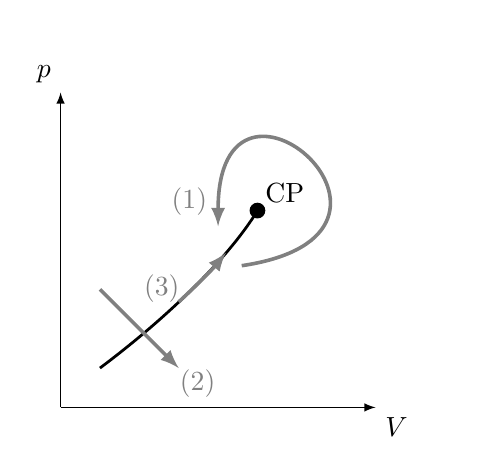
\begin{tikzpicture}
      \draw[-latex] (0,0) -- (4,0) node[below right] {$V$};
      \draw[-latex] (0,0) -- (0,4) node[above left] {$p$};
      \draw[line width=1pt] (0.5,0.5) .. controls (1.5,1.25) and (2.2,2.0) .. (2.5,2.5);
      \fill (2.5,2.5) circle (0.1) node[above right=-1pt] {CP};
      \draw[-latex,gray,line width=1.3pt] (0.5,1.5) -- (1.5,0.5) node[below right=-5pt] {$(2)$};
      \draw[-latex,gray,line width=1.3pt] (2.3,1.8) .. controls (5,2.2) and (2,4.8) .. (2,2.3) node[above left ] {$(1)$};
      \draw[-latex,gray,line width=1.3pt] (1.5,1.34) node[above left=-6pt]{$(3)$} .. controls (1.6,1.43) and (1.9,1.72) .. (2.1,1.965);
     \end{tikzpicture}
    }
    \caption{A szabadentalpia a nyomás függvényében (a), illetve speciális átalakulások a kritikus pont körül (b).}\label{fig:B09-gpspecatal}
   \end{figure}
    
   \paragraph{A kritikus pont körüli átalakulások} Speciális átalakulásokat mutat \aref{fig:B09-specatal}. ábra:

   \begin{enumerate}
    \item[(1)] Ekkor nem haladunk át fázishatáron, így a gőz/gáz/folyadék között nem látjuk sosem a különbséget.
   Ezen az úton nem történik fázisátalakulás, minden termodinamikai mennyiség analitikusan változik.
    \item[(2)] Áthaladunk a fázishatáron, elsőrendű fázisátalakulás történik.
   A fázishatáron különbséget látunk a folyadék és a gőz között, az egyik fázis moláris térfogata jóval nagyobb, mint a másiké. 
    \item[(3)] A fázishatáron haladva látjuk a különbséget a gőz és a folyadék között (a moláris térfogat különbözik).
   A kritikus pont felé haladva a sűrűségkülönbség csökken, és a kritikus pontban nullává válik.
   Ahogy áthaladunk a kritikus ponton, már csak egy fázist látunk.
   Mivel a $\Delta V$ folytonosan vált nullává, ez az átalakulás folytonos: másodrendű.
   \end{enumerate}

  \section{Univerzalitás}
   
   Lásd \aref{ss:B10-univerzalitas}. fejezetben.

  \chapter{Landau-elm\'elet, sk\'al\'az\'as} 
  
 
 \section{Rendparaméter}
   
  A rendparaméter ($\psi$) egy olyan mennyiség, aminek értékével közvetlenül jellemezni tudjuk azt, hogy melyik fázisban vagyunk. $\psi$ egy olyan mennyiség, ami a szimmetrikus fázisban nulla, a szimmetriasértőben pedig véges értéket vesz fel. Legyen $G_{sz}$ a szimmetrikus fázis csoportja, míg $G_{nsz}$ a szimmetriasértőé. Másodrendű az átalakulás, ha $G_{nsz}\subset G_{sz}$, ugyanis ekkor egy paraméter folytonos változtatásával elérhető, hogy a szimmetrikus fázis szimmetriacsoportja $G_{nsz}$-ra szűküljön. Ha $G_{nsz}\nsubseteq G_{sz}$, akkor az átalakulás biztos, hogy elsőrendű.
  
  A rendparaméterhez tartozik egy konjugált tér, mellyel el lehet érni, hogy a szimmetrikus fázisban is véges értéket vegyen fel. Ilyen pl.\ $H$ az FM--PM átalakulásnál, de nincs ilyen valós tér pl.\ az AFM--FM átalakulásnál. 
 
 \section{Landau-elmélet}
 
  A Landau-elmélet alapvető célja, hogy a szabadenergia(-sűrűség)-et felírja mint egy kis paraméter Taylor-soraként a kritikus pont közelében. Ez a kis paraméter a rendparaméter lesz. A ferromágneses--paramágneses átalakulás nyelvezetét használva ($\psi=m$) írjuk fel az elméletet. Az alapfeltevések a következőek:
  \begin{itemize}
   \item $\TC$ környékén a a mágnesezettségi sűrűsége nagyon pici: $m\xrightarrow{T\to\TC}0$,
   \item az állapotok eloszlása nagyon éles $m$ szerint, így az $m$ várható értéke és legvalószínűbb értéke megegyezik,
   \item illetve az eloszlások közelíthetőek Gauss-görbével. (Ez a fluktuációk meghatározásánál lesz hasznos.)
  \end{itemize}
  
  A (mágneses) szabadenergia-sűrűség sorfejtése negyedrendig:
  \al{
   f(T,H,m)=w(T)+\frac{a(T)}{2}m^2+\frac{u(T)}{4}m^4-Hm.
  }
  Mágneses tér nélkül az energia invariáns $m$ előjelétől, így $m$-nek csak páros hatványai szerepelhetnek. Minden hatvány együtthatója függhet $T$-től. Elvárjuk, hogy $u(T)$ pozitív legyen minden $T$-re, hogy létezzen globális minimum. 
  
  Egyensúly ott van, ahol $m$ minimalizálja $f$ értékét:
  \al{
   &0=\pder{f}{m}=a(T)m+u(T)m^3-H
   &0<\pder{^2 f}{m^2}=a(T)+3 u(T)m^2
  }
  
  $H=0$ esetben az $m=0$ jó megoldás. Az egyensúlyi feltétel akkor teljesül, ha $a(T)>0$.
  
  $m\ne 0$ megoldás esetében $m=\sqrt{-\frac{a(T)}{u(T)}}$. Az egyensúlyi feltétel: $0<a(T)+3 u(T)m^2=a(T)-3u(T)\frac{a(T)}{u(T)}=-2a(T)$, tehát itt $a(T)$ negatív. 
  
  Legyen $\TC$ az a hőmérséklet, ahol $a(T)$ előjelet vált. Legegyszerűbb közelítésben $a(T)=a_0(T-\TC)$ és $u(T)=u_0$. Az állapotegyenlet megoldását \aref{fig:B10-landau}. ábra mutatja.
  
  \begin{figure}[ht!]
   \centering
   \subfloat[Az állapotegyenlet megoldása $m(T,H)$-ra.\label{fig:B09-l1}]{\includegraphics[width= 0.5\textwidth]{./B09tetel/thm}} \\
   \subfloat[Fix mágneses tér mellet az $m(T)$ függvény.\label{fig:B09-l2}]{\includegraphics[width= 0.3\textwidth]{./B09tetel/TM}} \hspace{6pt}
   \subfloat[Fix hőmérséklet mellet az $m(H)$ függvény.\label{fig:B09-l3}]{\includegraphics[width= 0.3\textwidth]{./B09tetel/HM}} \hspace{6pt}
   \subfloat[Fix mágnesezettség mellet az $H(T)$ függvény.\label{fig:B09-l4}]{\includegraphics[width= 0.3\textwidth]{./B09tetel/HT}} 
   \caption{A negyedrendű szabadenergia sorfejtéssel felírt Landau-elmélet  állapotegyenlete és annak szintvonalai mindhárom síkra vetítve. Az (a) ábrán látszik, hogy hol hányadrendű az átalakulás: a $H=0$, $T<T_\text{C}$ vonalon $m=\pder{f}{H}$ ugrik, vagyis is elsőrendű az átalakulás, míg $H=0$, $T=T_\text{C}$-ben $m$ érintője, vagyis $\pder{^2 f}{H^2}$ vagy $\pder{^2 f}{H\partial T}$ vagy $\pder{^2 f}{T^2}$ divergál, vagyis az átalakulás abban a pontban másodrendű.}\label{fig:B10-landau}
  \end{figure}
  
  Vezessük be $\tau=T-\TC$-t, a relatív hőmérsékletet.
  Eddig tehát tudjuk, hogy
  \al{
   m=\begin{cases}
      0 & T<\TC\\
      \sqrt{\frac{a_0}{u_0}}\abs{\tau}^{\frac{1}{2}} & T>\TC,
     \end{cases}
  } 
  vagyis $\beta=\frac{1}{2}$.
  
  $T=\TC$-n a mágnesezettség tértől való függését is fel tudjuk írni. Az egyensúlyra vonatkozó egyenletek alapján:
  \al{
   &H=u_0m^3
   &m=\abs{\frac{H}{u}}^{\frac{1}{3}}\sim \abs{H}^\frac{1}{3},
  }
  ahonnan $\delta=\frac{1}{3}$.
  
  Az $m(T)$-ből a szuszceptibilitás, felhasználva az egyensúlyra vonatkozó egyenleteket:
  \al{
   \chi^{-1}=\pder{H}{m}=\pder{^2 f}{m^2}=a(T)+3 u(T)m^2
    =\begin{cases}
      T<\TC: &-2a(T)=2a_0\abs{\tau}\\
      T>\TC: &\phantom{-2}a(T)=a_0\abs{\tau}
     \end{cases}
  }
  vagyis s szuszceptibilitás divergál $T=\TC$-n, csak két oldalról kicsit más együtthatóval. Az exponens $\gamma=1$. 
  
  A szabadenergia az egyensúlyban és $H=0$ esetben:
  \al{
   F(T,H=0)
    &=\min_{M}F(T,H,M)
     =V\min_{m}\left(w(T)+\frac{a(T)}{2}m^2+\frac{u(T)}{4}m^4\right)\\
    &=\begin{cases}
       T<\TC:& V\left(w(T)-\frac{a_0^2\tau^2}{4u_0}\right) \\
       T>\TC:& Vw(T)
      \end{cases}
  }
  A hőkapacitás:
  \al{
   C_V=-T\pder{^2F }{T^2}
    =\begin{cases}
      T<\TC:& -TV\pder{^2 w(T)}{T^2}+TV\frac{a_0^2}{2u_0} \\
      T>\TC:& -TV\pder{^2 w(T)}{T^2}
     \end{cases}
  }
  vagyis $T=\TC$-n a fajhőnek ugrása van: $C(\TC-0)-C(\TC+0)=TV\frac{a_0^2}{2u_0}$, így a fajhő kritikus exponens $\alpha=0$.
  
  A fluktuációk számításához a paramágneses fázisban felhasználjuk, hogy $P(M)\sim e^{-\beta F(T,H,M)}$. $H=0$ esetben, csak a másodrendű tagot megtartva:
  \al{
   &P(M)\sim e^{-\beta V\frac{a(t)}{2}m^2}
   &\Rightarrow
   &&\mv{(\Delta m)^2}&=\frac{1}{\beta V a(T)}=\frac{\kB T}{V a(T)}=\frac{\kB T}{V}\chi\\
   &&&&\mv{(\Delta M)^2}&=\kB T V\chi.
  }
  
  A korrelációs függvény kiszámításához inhomogén mágneses teret és inhomogén mágnesezettséget kell bevezetni. Az $f$-ben $m=m_\text{eq}+\delta m(\rv)$, ahol $\delta m(\rv)$ a helyfüggő kis moduláció a mágnesezettségben. Ekkor a szabadenergia sorfejtésébe bele kell venni az $m(\rv)$ gradiensét is egy $\frac{c}{2}\abs{\grad{m(\rv)}}^2$ taggal. $f$ kifejtve, majd Fourier-transzformálva Gauss-alakú lesz, ahonnan a fluktuáció nagysága leolvasható. Innen a szuszceptibilitás kifejezhető:
  \al{
   &\chi(q)=\frac{1}{c}\frac{1}{q^2+\xi^{-2}}
   &\xi=\sqrt{\frac{c}{a(T)+3u_0m^2}}.
  }
  A korrelációs függvény:
  \al{
   &C(q)=\beta^{-1}\chi(q)
    =\frac{\kB T}{c}\frac{1}{q^2+\xi^{-2}}
   &C(r)=\frac{\kB T}{c}\frac{1}{4\pi}\frac{e^{-r/\xi}}{r},
  }
  így tehát $\xi$ a korrelációs hossz, mely
  \al{
   \xi^{-2}=\frac{1}{c}\big(a(T)+3u_0m^2\big)
    =\begin{cases}
      H=0, T<\TC, \left(m^2=-\frac{a(T)}{u_0}\right): & 2\frac{a_0\abs{\tau}}{c}\\
      H=0, T>\TC, \left(m=0\right): & \frac{a_0\abs{\tau}}{c}\\
      H\ne 0, T=\TC, \left(a=0,H=u_0m^3\right): & \frac{3u_0}{c}\left(\frac{H}{u_0}\right)^{\frac{3}{2}}
     \end{cases}
  }
  Inenn mindjárt látszik, hogy $H=0$-ra $\xi\sim \abs{\tau}^{-\nu}$, $\nu=\frac{1}{2}$. és $T=\TC$-re $\xi\sim \abs{H}^{-\mu}$, $\mu=\frac{1}{3}$. $C(q)$ $\tau=0$ és $H=0$-ra $C(r)\sim r^{-d+2-\eta}$, ahol $d=3$ a dimenziószám, így $\eta=0$.
  
 \section{Ginzburg-kritérium}
  
  A Landau-elmélet dimenziófüggetlen, de a fázisátalakulások nem azok. Nézzük meg, hogy a Landau-elmélet konzisztens-e. 
  
  Számoljuk ki a mágnesezettség fluktuációit:
  \al{
   \mv{\Delta M^2}
   &=\intl{V}{}\drh\intl{V}{}\drkh\mv{m(\rv)-m_\text{eq}}\mv{m(\rv')-m_\text{eq}}
    =\intl{V}{}\drh\intl{V}{}\drkh C(\rv-\rv')\\
   &=V\intl{V}{}\drh C(\rv)
    =VC(q=0)
    =V\kB T \chi(q=0)
    =V\kB T \chi
  }
  A relatív fluktuáció:
  \al{
   \frac{\mv{\Delta M^2}}{M^2}
    =\frac{V\kB T \chi}{M^2}
    =\frac{\kB T \chi}{V m^2}.
  }
  A korrelációk csak $\xi^d$ tartományban vannak, így a minta térfogata helyett ebben a térfogatban tekintsük a relatív fluktuációkat. Ekkor a hőmérséklettől való függés:
  \al{
   \frac{\mv{\Delta M^2}}{M^2}
    =\frac{\kB T \chi}{\xi^d m^2}
    \sim\frac{\abs{\tau}^{-1}}{\abs{\tau}^{-d/2}\cdot\abs{\tau}^{2\cdot 1/2}}
    \sim \abs{\tau}^{d/2-2}.
  }
  Az elmélet akkor használható, ha $\tau\to 0$-re a szabadenergia-sűrűség sorfejtése értelmes, azaz, ha a fluktuációk nem robbannak fel. Ehhez szükséges, hogy $d/2-2\ge 0$, vagyis $d\ge 4$. Tehát a Landau-elmélet szigorúan véve csak négy, vagy annál nagyobb dimenzióban értelmes.
  
  Praktikusan ez alacsony dimenzióban a Landau-elméletnek egy korlátot ad, hogy meddig érvényes. Annyira közelíthetjük meg $\TC$-t, hogy ez a fluktuációs tag még $\sim\mathcal{O}(1)$ legyen.
  
 \section{Skálahipotézis, skálázás}
  
  A sálahipotézis abból, áll, hogy feltesszük, hogy a rendszerben egyetlen karakterisztikus hosszúság van, a korrelációs hossz. 
  
  A korrelációs függvény ekkor: $C(q,\xi)=C(q=0,\xi)\cdot\phi(q\xi)$, ugyanis másképp nem függhet $q$-tól. Tudjuk, hogy $C(q=0)\sim\chi\sim\abs{\tau}^{-\gamma}$, illetve $\xi\sim\abs{\tau}^{-{\nu}}$, így $C(q=0)\sim\xi^{\frac{\gamma}{\nu}}$, vagyis
  \al{
   C(q,\xi)=\xi^{\frac{\gamma}{\nu}}\cdot\phi'(q\xi).
  }
  Ez egy általánosított homogén függvény, hiszen
  \al{
   &C\left(\lambda q,\frac{\xi}{\lambda}\right)
    &=\left(\frac{\xi}{\lambda}\right)^{\frac{\gamma}{\nu}}\phi'\left(\lambda q\frac{\xi}{\lambda}\right)
     =\lambda^{-\frac{\gamma}{\nu}}C\left(q,\xi\right)
   &\Rightarrow
   &&C\left(q,\xi\right)=\lambda^{\frac{\gamma}{\nu}}C\big(\lambda q,\lambda^{-1}\xi\big).
  }
  Visszaírva a $\tau$ függést: $\xi=\xi_0\abs{\tau}^{-\nu}$ $\rightarrow$ $\lambda^{-1}\xi=\xi_0\left(\lambda^{\frac{1}{\nu}}\abs{\tau}\right)^{-\nu}$, vagyis $C(q,\tau)=\lambda^{\frac{\gamma}{\nu}}C\big(\lambda q,\lambda^{\frac{1}{\nu}}\tau\big)$. 
  
  Teljesen hasonlóan le lehet vezetni a $H$-tól való függést $\xi$-n keresztül. Összegezve:
  \al{
   C\left(q,\tau,H\right)=\lambda^{\frac{\gamma}{\nu}}C\Big(\lambda q,\lambda^{\frac{1}{\nu}}\tau,\lambda^{\frac{1}{\mu}}H\Big),
  }
  ami még mindig egy hipotézis, csak jól argumentált. 
  A korrelációs függvényre hasonló skálahipotézis adható. Ez úgy adható meg, hogy $\xi$ az a távolság ami alatt a korrelációs függvény a felére csökken: $C(q=\frac{1}{\xi})=\frac{1}{2}C(q=0)$, ennek kifejtéséből:
  \al{
   \xi(\tau,H)=\lambda \xi\Big(\lambda^{\frac{1}{\nu}}\tau,\lambda^{\frac{1}{\mu}}H\Big).
  }
  A korrelációs függvényre vonatkozó skálahipotézisből a szuszceptibilitás ($\chi=\beta C(q=0)$): $\chi(\tau,H)=\lambda^{\frac{\gamma}{\nu}}C\big(\lambda^{\frac{1}{\nu}}\tau,\lambda^{\frac{1}{\mu}}H\big)$, ahol $\lambda'=\lambda^{\frac{1}{\nu}}$-t bevezetve
  \al{
   \chi(\tau,H)=\lambda^{\gamma}\chi\Big(\lambda\tau,\lambda^{\frac{\nu}{\mu}}H\Big). 
  }
  A mágnesezettség: $\chi=\pder{m}{H}$, vagyis akkor 
  \al{
   m(\tau,H)=\lambda^{\gamma-\frac{\nu}{\mu}}m\Big(\lambda\tau,\lambda^{\frac{\nu}{\mu}}H\Big)
  }
  kell, hogy legyen. Hasonlóan a szabadenergia-sűrűség:
  \al{
   f(\tau,H)=\lambda^{\gamma-2\frac{\nu}{\mu}}f\Big(\lambda\tau,\lambda^{\frac{\nu}{\mu}}H\Big).
  }
  
  \subsection{Összefüggések a kritikus exponensek között}
   \begin{itemize}
    \item A korrelációs hossz, ha $H=0$, és $\lambda=\abs{\frac{\tau}{\tau_0}}^{-\nu}$:
    \al{
     \xi(\tau,0)
      =\lambda \xi\Big(\lambda^{\frac{1}{\nu}}\tau,0\Big)
      =\abs{\frac{\tau}{\tau_0}}^{-\nu} \xi\left(\abs{\frac{\tau}{\tau_0}}^{\frac{-\nu}{\nu}}\tau,0\right)
      =\abs{\frac{\tau}{\tau_0}}^{-\nu} \underbrace{\xi\Big(\pm\tau_0,0\Big)}_{=\text{konst}}
      \sim \abs{\tau}^{-\nu},
    }
    illetve ha $\tau=0$ és $\lambda=\abs{\frac{H}{H_0}}^{-\mu}$:
    \al{
    \xi(0,H)
     =\lambda \xi\Big(0,\lambda^{\frac{1}{\mu}}H\Big)
     =\abs{\frac{H}{H_0}}^{-\mu} \xi\left(0,\abs{\frac{H}{H_0}}^{\frac{-\mu}{\mu}}H\right)
     =\abs{\frac{H}{H_0}}^{-\mu} \underbrace{\xi\left(0,\pm H_0\right)}_{=\text{konst}}
     \sim \abs{H}^{-\mu}.
    }
    
    \item A szuszceptibilitás $H=0$-ra és $\lambda=\abs{\frac{\tau_0}{\tau}}$-t választva:
    \al{
     \chi(\tau,0)
      =\lambda^{\gamma}\chi\Big(\lambda\tau,0\Big)
      =\abs{\frac{\tau_0}{\tau}}^{\gamma}\chi\Big(\abs{\frac{\tau_0}{\tau}}\tau,\lambda^{\frac{\nu}{\mu}}H\Big)
      =\abs{\frac{\tau_0}{\tau}}^{\gamma}\underbrace{\chi\Big(\pm\tau_0,0\Big)}_{=\text{konst}}
      \sim\abs{\tau}^{-\gamma}
    }
    
    \item A korrelációs függvény $\tau=0$ és $H=0$-ra, $\lambda=\frac{q_0}{q}$ választással
    \al{
     C\left(q,0,0\right)
      =\lambda^{\frac{\gamma}{\nu}}C\Big(\lambda q,0,0\Big)
      =\left(\frac{q_0}{q}\right)^{\frac{\gamma}{\nu}}C\left(\frac{q_0}{q} q,0,0\right)
      =\left(\frac{q_0}{q}\right)^{\frac{\gamma}{\nu}}\underbrace{C\left(q_0,0,0\right)}_{=\text{konst}}
      \sim q^{-\frac{\gamma}{\nu}}.
    }
    Az $\eta$ kritikus exponenst úgy definiáltuk, hogy $C(q)\sim q^{-2+\eta}$, így $-2+\eta=-\frac{\gamma}{\nu}$ azonnal adódik.
    
    \item A mágnesezettségi sűrűségből $H=0$ esetben $\lambda=\abs{\frac{\tau_0}{\tau}}$-t választva:
    \al{
     m(\tau,0)
      =\lambda^{\gamma-\frac{\nu}{\mu}}m\Big(\lambda\tau,0\Big)
      =\abs{\frac{\tau_0}{\tau}}^{\gamma-\frac{\nu}{\mu}}m\Big(\abs{\frac{\tau_0}{\tau}}\tau,0\Big)
      =\abs{\frac{\tau_0}{\tau}}^{\gamma-\frac{\nu}{\mu}}\underbrace{m\Big(\pm\tau_0,0\Big)}_{=\text{konst}}
      \sim \abs{\tau}^{-\gamma+\frac{\nu}{\mu}}.
    }
    Szintén a korábbi $\beta$ exponens definíciójából $\beta=-\gamma+\frac{\nu}{\mu}$. Hasonlóan $\tau=0$, $
    \lambda=\abs{\frac{H_0}{H}}^{-\frac{\mu}{\nu}}$.
    \al{
     m(0,H)
      &=\lambda^{\gamma-\frac{\nu}{\mu}}m\Big(0,\lambda^{\frac{\nu}{\mu}}H\Big)
      =\abs{\frac{H_0}{H}}^{-\frac{\mu}{\nu}\gamma+1}m\Big(0,\abs{\frac{H_0}{H}}H\Big)
      =\abs{\frac{H_0}{H}}^{-\frac{\mu}{\nu}\gamma+1}\underbrace{m\Big(0,\pm H_0\Big)}_{=\text{konst}}\\
      &\sim\abs{H}^{\frac{\mu}{\nu}\gamma-1}.
    }
    Szintén a korábbi definícióval való összevetésből: $\frac{1}{\delta}=-\frac{\mu}{\nu}\gamma+1$.
    
    \item Végül a fajhőhöz $f$, ha $H=0$: válasszuk $\lambda=\abs{\frac{\tau_0}{\tau}}$,
    \al{
     f(\tau,0)
     &=\lambda^{\gamma-2\frac{\nu}{\mu}}f\Big(\lambda\tau,0\Big)
      =\abs{\frac{\tau_0}{\tau}}^{\gamma-2\frac{\nu}{\mu}}f\Big(\abs{\frac{\tau_0}{\tau}}\tau,0\Big)
      =\abs{\frac{\tau_0}{\tau}}^{\gamma-2\frac{\nu}{\mu}}\underbrace{f\Big(\pm\tau_0,0\Big)}_{=\text{konst}}
      \sim \abs{\tau}^{-\gamma+2\frac{\nu}{\mu}}.
    }
    Innen a fajhő $\tau$ függése megadható, hiszen az a szabadenergia-sűrűség második deriváltjával arányos. A két deriválás a kitevőben $-2$-t hoz be, így $C\sim\pder{^2 f}{T^2}\sim \abs{\tau}^{-\gamma+2\frac{\nu}{\mu}-2}$. A korábbi definíció alapján így: $\alpha=\gamma-2\frac{\nu}{\mu}+2$. Ennek az egyenlőségnek az átírásához felhasználjuk a $\beta$-ra vonatkozó egyenletet: $\alpha=-2\beta-\gamma+2$.
   \end{itemize}
   
   Összefoglalva:
   \al{
     C&\sim\abs{\tau}^{-\alpha} && H=0\\
     m&\sim\abs{\tau}^{\beta} && H=0\\
     \chi&\sim\abs{\tau}^{-\gamma} && H=0\\
     m&\sim\abs{H}^{\frac{1}{\delta}} && \tau=0\\
     \xi&\sim\abs{\tau}^{-\nu} && H=0\\
     \xi&\sim\abs{H}^{-\mu} && \tau=0\\
     C(q)&\sim \frac{1}{q^{2-\eta}} \;\Leftrightarrow \; C(r)\sim \frac{1}{r^{d-2+\eta}}&& \tau=0,H=0,
   }
   illetve a skálatörvények:
   \al{
    &\gamma=\nu(2-\eta)
    &\beta=-\gamma+\frac{\nu}{\mu}
    &&\frac{1}{\delta}=\frac{\nu-\mu\gamma}{\nu}
    &&2-\alpha=2\beta+\gamma.
   }
   Tehát $\gamma,\mu,\nu$-vel ki lehet fejezni az összes exponenst. Ez a három exponens határozza meg az univerzalitási osztályokat. 
   \paragraph{Hiperskálatörvény}
    
    Ezeken felül még egy skálatörvény belátható, ami a dimenziószámot is figyelembe veszi. A Ginzburg-kritériumnál láttuk, hogy 
    \al{
     \frac{\mv{\Delta M^2}}{M^2}
    =\frac{\kB T \chi}{V m^2}.
    }
    
    Azt láttuk, hogy egy korrelációs hossznyi tartományban ez csak akkor nem divergál $T\to\TC$-re, ha $d\ge 4$. Ha ez mégis divergálna, akkor létezne egy nagyobb térfogat, $R^d$, ahol a relatív fluktuáció $\sim\mathcal{O}(1)$. De ez ellentmondás, mert a skálahipotézis kimondja, hogy nem létezik más karakterisztikus távolság, csak $\xi$, úgyhogy annak kell igaznak lennie, hogy 
    \al{
    \mathcal{O}(1)\sim
     \frac{\kB T \chi}{\xi^d m^2}
     \sim\frac{\abs{\tau}^{-\gamma}}{\abs{\tau}^{-d\nu}\cdot\abs{\tau}^{2\cdot \beta}}
    \sim \abs{\tau}^{d/\nu-2\beta-\gamma},
    }
    vagyis $d/\nu-2\beta-\gamma=0$, ahonnan a hiperskálatörvény:
    \al{
     d\nu=2\beta+\gamma.
    }
    Az Ising-exponensekkel így az jön ki, hogy a Landau-elmélet csak $d=4$ dimenzióban korrekt.
    
 
 \section{Univerzalitás}\label{ss:B10-univerzalitas}
  
  A másodrendű fázisátalakulások rengeteg rendszerben jelen vannak. A megfigyelés az, hogy látszólag teljesen különböző rendszerek is ugyanazt a viselkedést mutatják a kritikus pont közelében. 
  
  Ennek magyarázata az, hogy ahogy a rendszer egyre közelebb kerül a kritikus ponthoz, úgy az egyre inkább skálafüggetlenné válik. Emiatt a rendszernek minden skáláfüggő tulajdonsága elvész, és csak a néhány releváns, skálafüggetlen tulajdonság marad. 
  
  A kritikus pont közelében a rendszerek hasonlósága abban nyilvánul meg, hogy a kritikus exponensek megegyeznek. Ez alapján a hasonló rendszereket univerzalitási osztályokba lehet sorolni. Az XY-osztályba tartozik például az az XY-Heisenbeg-model, a szupravezetés és a szuperfolyékonyság; az Ising-osztályba tartozik az Ising-modell, a folyadék--gáz fázisátalakulások és az uniaxiális mágnesek. A Heisenberg-osztályba az izotrop mágnesek és a Heisenberg-modell. 
  
  
  
  \include{B11tetel/B11tetel}
  \chapter{Transzport, fluktu\'aci\'ok, id\H{o}f\"ugg\H{o} korrel\'aci\'ok, kereszteffektusok, Onsager-rel\'aciok} 
 
 \section{Időfüggő egyensúlyi korrelációs függvények}
  
  Legyen két időfüggő fizikai mennyiség $X(t)$ és $Y(t)$.
   Ezek átlaguktól való eltérése: $x(t)=X(t)-\mv{X}(t)$ és $y(t)=Y(t)-\mv{Y}(t)$.
   Az időfüggő korrelációs függvény:
  \al{
   C_{xy}(t)=\mv{x(t')y(t'+t)}_{t'}
    =\lim_{T\to\infty}\frac{1}{T}\intl{0}{T}\dd t'\, x(t')y(t+t').
  }
  Ha a rendszer stacioner és ergodikus, akkor az így definiált időátlag, $\mv{\,\cdot\,}_{t'}$, megegyezik a sokaságátlaggal, $\mv{\,\cdot\,}$.
   A korrelációs függvény tulajdonságai:
  \begin{itemize}
   \item 
    $t\to\infty$-re a korrelációk függetlenek lesznek egymástól:
    \al{
     \lim_{t\to\infty}C_{xy}(t)
      &=\lim_{t\to\infty}\mv{x(t')y(t'+t)}_{t'}
       =\lim_{t\to\infty}\mv{x(0)y(t)}
       =\mv{x(0)}\lim_{t\to\infty}\mv{y(t)}
       =0
    }
    
   \item
    $t=0$-ra az időfüggő korrelációs függvény megegyezik a keresztkorrelációs együtthatókkal:
    \al{
     C_{xy}(t=0)
      &=\mv{x(t')y(t')}_{t'}
       =\mv{x(0)y(0)}
    }
    
   \item 
    \al{
     C_{xy}(t)
      &=\mv{x(t')y(t'+t)}_{t'}
       =\mv{x(t'-t)y(t')}_{t'}
       =\mv{y(t')x(t'+(-t))}_{t'}
       =C_{yx}(-t)
    }
   \item 
    A korrelációs függvény szimmetrikus: $C_{xy}(t)=C_{yx}(t)$ (ha a rendszer időtükrözésre invariáns).
   Ehhez fejtsük ki a fenti sokaságátlagot:
    \al{
     C_{xy}(t)
      &=\intl{}{}\dd x\,\intl{}{}\dd y\, xy\cdot P(x) P(y,t|x) ,
    }
    ahol $P(x)$ annak a valószínűsége, hogy $x$ fluktuációja $x$, illetve $P(t,y|0,x) $ annak a valószínűsége, hogy $y$ a fluktuáció értéke $t$-ben, ha $t=0$-ban $x$ értéke $x$ volt.
   A részletes egyensúly következménye, hogy $P(x) P(t,y|0,x)=P(y) P(t,x|0,y)$.
   Ezt behelyettesítve:
    \al{
     C_{xy}(t)
      &=\intl{}{}\dd x\,\intl{}{}\dd y\, xy\cdot P(y) P(t,x|0,y)
       =C_{yx}(t).
    }
   
   \item 
    Az előző kettőből $C_{yx}(t)=C_{xy}(-t)$, vagyis a korrelációs függvény időben is szimmetrikus. 
  \end{itemize}
  
  A korrelációs függvények kiterjeszthetőek a kvantummechanikai esetre is.
   Itt azonban figyelembe kell venni, hogy az operátorok nem felcserélhetőek.
   Ehhez szimmetrizálni/antiszimmetrizálni kell:
  \al{
   C^{F/B}_{\opx\opy}=\frac{1}{2}\mv{\mv{\opx(t')\opy(t'+t)\pm\opy(t'+t)\opx(t')}}_{t'}.
  } 
  A belső várható érték a kvantummechanikai várható értéket jelenti, a külső pedig az időbelit.
   Az előbb bizonyított tulajdonságok továbbra is fennállnak. 
  
 \section{Lineáris transzport}
  
  Egyensúlyban a fluktuációk várható értéke nulla, azonban az értékük az egyes időpillanatokban nem nulla.
   Az fluktuáció oka a statisztikus jelleg, az, hogy az eloszlásnak van valamilyen szélessége.
   A fluktuáció véges értékét úgy is el tudjuk érni, hogy a rendszerre valamilyen külső teret kapcsolunk, majd ezt a teret kikapcsoljuk.
   Amíg a teret bekapcsoltuk, a rendszerbe beleavatkoztunk, így az nem-egyensúlyi állapotban van.
  
  Bárhogy is jött létre az átlagértéktől való eltérés, a várható értéke $t\to\infty$-re újra lecseng:
  \al{
   \lim_{t\to\infty}\mv{\xv(t)|\xv(t=0)=\xv_0}=0.
  }
  
  A nem egyensúlyi sokaságok lényege, hogy a valamilyen módon előállt $x_0$ makroállapotnak megfelelő sokaságot állítjuk elő, azzal a feltételes eloszlással, hogy $x_0$ fennáll.
   A rendszerben a dinamika változatlan, egyedül az eloszlás különbözik. 
  
  Térítsünk ki egy mennyiséget az egyensúlyi értékéből.
   Az átlaghoz való visszatérési sebessége ekkor arányos lesz a kitéréssel, vagyis:
  \al{
   \mv{\dot x_i}_{\xv_0}=-\suml{k}{}\lambda_{ik}\mv{x_k}_{\xv_0}.
  }
  Definiáljunk a termodinamikai erőt: $y_i=-\pder{S}{x_i}$.
   Az entrópia sorfejtése: $S=S_0-\frac{1}{2}\suml{ij}{}x_ig_{ij}x_j$, ahol $g_{ij}$ szimmetrikus.
   Innen $y_i=\suml{j}{}g_{ij}x_j$, ami megfordítva $x_i=\suml{j}{}\big[g^{-1}\big]_{ij}y_j$.
   Ezt felhasználva:
  \al{
   \mv{\dot x_i}_{\xv_0}
    =-\suml{k}{}\lambda_{ik}\suml{j}{}\big[g^{-1}\big]_{kj}\mv{y_j}_{\xv_0}
    =-\suml{j}{}\underbrace{\suml{k}{}\lambda_{ik}\big[g^{-1}\big]_{kj}}_{L_{ij}}\mv{y_j}_{\xv_0}
    =-\suml{j}{}L_{ij}\mv{y_j}_{\xv_0}
  }
  Ez a transzportegyenlet.
   A termodinamikai erőre másik definíciót is adhatunk.
   Az előző alapján felírhatjuk, hogy $\dd S=-\suml{i}{}y_i\dd x_i$.
   Innen az entrópiaprodukció: $\dot S=-\suml{i}{}y_i\dot x_i$, vagyis $y_i=-\pder{\dot S}{\dot x_i}$. 
  
  \subsection{Onsager-hipotézis}
   
   Az Onsager-hipotézis lényege, hogy az egyensúlyi fluktuációk és a nem egyensúlyi kitérítés között nincs különbség, miközben a rendszer relaxál mindegy, hogy mi volt az eredeti kitérés oka.
   Ez azt jelenti, hogy a transzportegyenlet a korrelációs függvényekre felírva is igaz:
   \al{
    \der{}{t}\mv{x_i(t),x_j(0)}=-\suml{k}{}L_{ik}\mv{y_k(t),x_j(0)}.
   }
   A hipotézis következményének belátásához felhasználjuk a korrelációs függvény szimmetrikusságát ($C_{ij}(t)=C_{ji}(t)$), illetve az alábbi azonosságot: $\mv{y_k x_j}=\kB\delta_{kj}$.
   Ennek belátásához nézzük a 
   \al{
    0
     &=N\intl{}{}\dd^{n}x\,\pder{}{x_j}\left(x_i e^{-\frac{1}{2\kB}\suml{lm}{}x_l g_{lm}x_m}\right)\\
     &=N\intl{}{}\dd^{n}x\,\underbrace{\pder{x_i}{x_j}}_{\delta_{ij}} e^{-\frac{1}{2\kB}\suml{lm}{}x_l g_{lm}x_m}+N\intl{}{}\dd^{n}x\,x_i\pder{}{x_j} e^{-\frac{1}{2\kB}\suml{lm}{}x_l g_{lm}x_m}\\
     &=\delta_{ij}+N\intl{}{}\dd^{n}x\,x_i \left(-\frac{1}{\kB}\suml{l}{} g_{jl}x_l\right)e^{-\frac{1}{2\kB}\suml{lm}{}x_l g_{lm}x_m}
      =\delta_{ij}-\frac{1}{\kB}\mv{x_i y_j}.
   }
   Az első egyenlőség triviálisan igaz, hiszen ha $x_j$ szerint kiintegrálunk, akkor az kiintegrált rész eltűnik a határokon. 
   
   Tehát használjuk fel a korrelációs függvény szimmetrikusságát:
   \al{
    &\der{}{t}\mv{x_i(t),x_j(0)}=\der{}{t}\mv{x_j(t),x_i(0)}
    &\Rightarrow&
    &-\suml{k}{}L_{ik}\mv{y_k(t),x_j(0)}=-\suml{k}{}L_{jk}\mv{y_k(t),x_i(0)},
   }
   majd tekintsük a relációt $t=0$-ban.
   Ekkor felhasználva a másik azonosságot:
   \al{
    L_{ij}=L_{ji}
   }
   adódik, ami az Onsager-féle reciprocitási törvény.
   Mivel a korrelációs törvény szimmetrikusságának követelménye az volt, hogy a mikroszkopikus folyamatok reverzibilisek, ezért ezt itt is meg kell követelni.
   Az időtükrözési invariancia lehetséges, hogy nem teljesül pl. mágneses tér jelenlétében, vannak olyan mennyiségek, amelyek előjelet váltanak az időtükrözésre.
   Ekkor $C_{xy}(t)=I_x I_y C_{yx}(t)$, ahol $I$ az időtökrözéshez tartozó sajátérték, és így $L_{xy}=I_x I_y L_{yx}$.
   
  \subsection{Példa: hő- és elektromos vezetés}
   
   \begin{description}
    \item[Elektromos vezetés:] Az entrópiaprodukció: $\der{S}{t}=\frac{P}{T}=\frac{EJ}{T}$, ahol $E$ az elektromos térerősség, $J$ az elektromos áramsűrűség és $T$ a hőmérséklet.
   A fenti jelöléssel $\dot x_e=J$.
   Az ehhez tartozó termodinamikai erő: $y_e=-\pder{\dot S}{\dot x_e}=-\frac{E}{T}$.
    
    Ezek alapján a transzportegyenlet: 
    \al{
     J=-L_{ee}\left(-\frac{E}{T}\right).
    }
    Ez az Ohm-törvény, ahol $L_{ee}=\sigma T$.
    
    \item[Hővezetés: ] Az entrópiaprodukció itt arányos a hőárammal és a hőmérséklet inverzének gradiensével: $\dot S=w\nabla\frac{1}{T}$.
   Innen $\dot x_{q}=w$, vagyis $y_q=-\pder{\dot S}{\dot x_{q}}=-\grad\frac{1}{T}=\frac{1}{T^2}\nabla T$.
    
    Itt a transzportegyenlet:
    \al{
     w=-L_{qq}\frac{1}{T^2}\nabla T,
    }
    ami a hővezetési egyenletnek felel meg $L_{qq}=\lambda T^2$.
    
    \item[Kereszteffektusok: ] Az elektromos áram létrehozhat hőáramot, illetve fordítva.
   Ezeket is figyelembe véve a transzportegyenletek:
    \al{
     J&=-L_{ee}\left(-\frac{E}{T}\right)-L_{eq}\frac{1}{T^2}\nabla T
      &
     E&=\frac{1}{\sigma}J+\eta\nabla T\\
     w&=-L_{qe}\left(-\frac{E}{T}\right)-L_{qq}\frac{1}{T^2}\nabla T
      &
     w&=\pi J-\lambda\nabla T
    }
    A jobb oldalon a korábbi ``kísérleti'' törvények állnak, $\pi$ a Peltier-együttható, míg $\eta$ a Seebeck-együttható.
   A kísérletek alapján a Thomson-összefüggés: $\pi=\eta T$.
   Ha $\grad T=0$, akkor $\pi=\frac{w}{J}=\frac{L_{qe}}{L_{ee}}$, illetve ha $J=0$, akkor $\eta=\frac{L_{eq}}{L_{ee}T}$.
   A Thomson-összefüggésbe helyettesítve $L_{eq}=L_{qe}$.
   \end{description}

  \chapter{Brown-mozg\'as, Langevin- \'es Fokker--Plack-egyenlet}
 
 \section{Brown-mozgás}
  
  A Brown-mozgás egy véletlen bolyongásnak tekinthető azon az idő és méretskálán, ahol az egyedi részecske-részecske ütközések már nem láthatóak.
   Egy kísérlet csak egy megvalósulást mutat, valójában a lehetséges mintázatok egy sokaságot alkotnak, amelyhez tartozik egy valószínűségi eloszlás is.
  
  \subsection{A Brown-mozgás klasszikus leírása}
   
   Készítsünk egy sokaságot, ahol a részecskék egydimenziós térben mozognak nehézségi erőtérben.
   Legyen a részecskék sűrűsége $n(t,x)$, míg az áramsűrűség pedig $j(t,x)$.
   Mivel a részecskék száma állandó, így $\partial_t n(t,x)+\partial_x j(t,x)=0$. 
   
   A részecskék mozgását két áramsűrűség határozza meg.
   Az egyik a diffúzió, ahol a Fick-törvény adja meg az áramsűrűség és a sűrűség közötti kapcsolatot: $j_\text{D}=-D\partial_x n(t,x)$.
   A másik oka a nehézségi erőtér és a közegellenállás által kifejtett erő.
   A mozgásegyenlet $m\ddot x_i=-m\gamma\dot x_i+F$, ahol ha az $\ddot a\approx 0$ (stacioner) esetet nézzük: $\dot x_i=\frac{F}{m\gamma}$.
   Az innen adódó áramsűrűség: $j_ F=n\cdot \dot x_i=\frac{nF}{m\gamma}$. 
   
   Az áramokat behelyettesítbe a sűrűségre kapunk egy differenciálegyenletet:
   \aln{
    \partial_t n(t,x)=-\frac{F}{m\gamma}\partial_x n+D\partial^2_x n(t,x).\label{eq:B13-mozge}
   }
   Stacioner állapotban az időfüggés eltűnik, így 
   \al{
    \frac{F}{m\gamma}n'(x)=D n''(x).
   }
   Nehézségi erőtérben ennek a megoldása $n(x)=n(x_0)e^{-\frac{mg}{D m\gamma}x}$.
   A megoldásnak meg kell felenie a Maxwell--Boltz\-mann-eloszlásnak, ami $n(x)=n(0)e^{-\frac{mgx}{\kB T}}$.
   Ennek következménye, hogy $D=\kB T\mu$, ahol $\mu$ a mozgékonyság, $\mu=\frac{\dot x_i}{F}=\frac{1}{m\gamma}$.
   
   Ez a fluktuáció--disszipáció-tétel megjelenése, a mobilitás, mint a külső térre adott válasz megjelenik, míg a disszipáció a diffúziós állandóval kapcsolatos. 
   
  \subsection{A Brown-mozgás valószínűségi leírása}
   
   Legyen $P(t,x|t_0,x_0)$ annak a valószínűsége, hogy a részecske a $t$ időpontban az $x$ helyen van, feltéve, hogy a $t_0$ pillanatban $x_0$-ban volt. \Eqaref{eq:B13-mozge} egyenletet fel lehet írni ezekre a valószínűségekre.
   Az $F=0$-t választva:
   \al{
    \partial_t P(t,x|t_0,x_0)=D\partial^2_x P(t,x|t_0,x_0).
   }
   Az egyenlet kezdeti feltétele: $P(t_0,x|t_0,x_0)=\delta(x-x_0)$.
   Az egyenlet megoldható, a megoldás egy Gauss-eloszlás, melynek szórása időben gyökösen nő:
   \al{
    &P(t,x|t_0,x_0)=\frac{1}{\sqrt{2\pi\sigma^2(t)}}e^{-\frac{(x-x_0)^2}{2\sigma^2(t)}}
    &\sigma(t)=\sqrt{2D(t-t_0)}.
   }
   
 \section{Langevin-egyenlet}
  
  A mozgásegyenletet kicsit átértelmezzük, ez a Langevin-egyenlet:
  \aln{
   \dot v(t)=-\gamma v(t)+\varphi(t).\label{eq:B13-langevin}
  }
  Itt az első tag a viszkozitásnak felel meg, míg a második a részecskékkel való ütközésnek felel meg.
   Ez az egyenlet egy sztochasztikus differenciálegyenlet, melynek megoldása egy eloszlás minden egyes időpillanatra, és tartalmazza a különböző időpontokhoz tartozó eloszlások közötti korrelációkat is. 
  
  A megoldáshoz Fourier-transzformáljuk a fenti egyenletet ($\partial_t\to -i\omega$):
  \al{
   -i\omega v(\omega)&=-\gamma v(\omega)+\varphi(\omega)\\
   v(\omega)&=\frac{\varphi(\omega)}{-i\omega +\gamma}\\
   \abs{v(\omega)}^2&=\frac{\abs{\varphi(\omega)}^2}{\omega^2 +\gamma^2}
  }
  
  Az egyenletben szereplő abszolút érték négyzetek éppen a spektrális sűrűségnek felelnek meg.
   A Wiener--Khintchin-tétel (\ref{ss:B11-fdt}. fejezet) alapján a spektrális sűrűség megegyezik a korrelációs függvény Fourier-transzformáltjával:
  \aln{
   \abs{v(\omega)}^2=S_{vv}(\omega)=C_{vv}(\omega)=\frac{S_{\varphi\varphi}(\omega)}{\omega^2 +\gamma^2}.\label{eq:B13-lange2}
  }
  A továbbiakhoz a sztochasztikus erőre kell feltételezéseket tennünk. 
  \begin{itemize}
   \item A sztochasztikus erőnek nincs kitüntetett iránya: $\mv{\varphi(t)}=0$.
   \item A molekulákkal való ütközés az általunk vizsgált időskálán korrelálatlan: \al{
    C_{\varphi\varphi}(t-t')=\mv{\varphi(t)\varphi(t')}=C\delta(t-t').
   }
   A prefaktor a Wiener--Khintchin-tétel alapján kapható: $S_{\varphi\varphi}(\omega)=\intl{}{}\dd\omega\,e^{i\omega t}C_{\varphi\varphi}(t)=C=S_{\varphi\varphi}$.
   A spektrális sűrűség tehát frekvenciafüggetlen.
  \end{itemize}
  
  Ezek alapján \eqaref{eq:B13-lange2} egyenlet időbe visszatranszformálva:
  \al{
   C_{vv}(t)
    =\frac{1}{2\pi}\intl{}{}\dd \omega\, e^{-i\omega t}\frac{S_{\varphi\varphi}}{\omega^2 +\gamma^2}
    =\frac{S_{\varphi\varphi}}{2\pi}\intl{}{}\dd \omega\, \frac{e^{-i\omega t}}{\omega^2 +\gamma^2}
    =\frac{S_{\varphi\varphi}}{2\gamma}e^{-\gamma\abs{t}}.
  }
  Az integrálás pl. a reziduum-tétellel viszonylag egyszerűen elvégezhető. $S_{\varphi\varphi}$ értéke a $t=0$-ban meghatározható, hiszen $C_{vv}(t=0)=\mv{v^2}$, ami pedig az ekvipartíció tétele miatt $\frac{1}{2}m\mv{v^2}=\frac{1}{2}\kB T$.
   Ezzel tehát:
  \al{
   &S_{\varphi\varphi}=\frac{2\gamma\kB T}{m}
   &C_{vv}(t)=\frac{\kB T}{m}e^{-\gamma\abs{t}}
  }
  
  A várható eltávolodásnégyzet:
  \al{
   \mv{(x(t)-x_0)^2}
    &=\mv{\left(\intl{0}{t}\dd t'\,v(t')\right)^2}
     =\intl{0}{t}\dd t'\,\intl{0}{t}\dd t''\,\mv{v(t')v(t'')}
     =\intl{0}{t}\dd t'\,\intl{0}{t}\dd t''\,C_{vv}(t'-t'')\\
    &=\frac{\kB T}{m}\intl{0}{t}\dd t'\,\intl{0}{t}\dd t''\,e^{-\gamma\abs{t'-t''}}
     =\frac{2\kB T}{m}\intl{0}{t}\dd t'\,\intl{t'}{t}\dd t''\,e^{-\gamma(t''-t')}\\
    &=-\frac{2\kB T}{m\gamma}\intl{0}{t}\dd t'\,\left[e^{-\gamma(t''-t')}\right]_{t'}^{t}
     =\frac{2\kB T}{m\gamma}\intl{0}{t}\dd t'\,\left(1-e^{-\gamma(t-t')}\right)\\
    &=\frac{2\kB T}{m\gamma}\left(t-\frac{1}{\gamma}\left(1-e^{-\gamma t}\right)\right).
  }
  
  Kis időkre az exponenciális sorfejtéséből $\sim t^2$-es időfüggést, míg nagy távolságokra $\sim t$-s időfüggést kapunk az eltávolodás négyzetének várhatóértékére.
   Rövid időre a részecske ballisztikus, majd a viszkozitás lelassítja, és a korábban kapott négyzetgyökös időfüggéssel távolodik el. 
  
  \section{Markov-folyamatok, master-egyenlet}
   
   Markov-folyamatok azok a folyamatok, melyeknek nincs memóriájuk, vagyis a rendszer állapota a következő pillanatban csak attól függ, hogy a rendszernek milyen most az állapota, attól nem hogy milyen volt.
   Ez a feltételes valószínűségekkel $t_n>t_{n-1}\dots t_1$:
   \al{
    P\big(t_{n+1},x_{n+1}\big|t_{n}x_{n};t_{n-1}x_{n-1};\dots;t_{1}x_{1}\big)
     =P\big(t_{n+1},x_{n+1}\big|t_{n}x_{n}\big),
   }
   vagyis ha van egy feltételünk $t_n$-ben, akkor a valószínűség a korábbi időpontokban megadott feltételektől független.
   
   Felhasználva a feltételes valószínűségek definícióját (FVD), a teljes valószínűségek tételét (TVT) és a Markov-folyamatok memóriavesztését (MEM):
   \al{
    \intl{}{}\dd x_2\,P(t_3,x_3;t_2,x_2;t_1,x_1)
     &\stackrel{\text{TVT}}{=}P(t_3,x_3;t_1,x_1)\\
     &\stackrel{\text{FVD}}{=}\intl{}{}\dd x_2\,P(t_3,x_3|t_2,x_2;t_1,x_1)P(t_2,x_2|t_1,x_1)P(t_1,x_1)\\
     &\stackrel{\text{MEM}}{=}\intl{}{}\dd x_2\,P(t_3,x_3|t_2,x_2)P(t_2,x_2|t_1,x_1)P(t_1,x_1)\\
    P(t_3,x_3|t_1,x_1)
     &=\intl{}{}\dd x_2\,P(t_3,x_3|t_2,x_2)P(t_2,x_2|t_1,x_1)
   }
   Az utolsó egyenlet a Chapman--Kolmogorov-egyenlet. 
   
   \paragraph{Master-egyenlet}
    
    Induljunk ki a következő azonosságból:
    \al{
     P(t_1+\tau,x_2)=\intl{}{}\dd x_1\,P\big(t_1+\tau,x_2|t_1,x_1\big)P(t_1,x_1),
    }
    ami azt fejezi ki, hogy annak a valószínűsége, hogy $\tau$ idővel később $x_2$-ben leszünk annyi, mint hogy feltesszük, hogy $t_1$-ben voltunk valahol, és integrálunk arra a feltételre, hogy voltunk valahol. 
    
    A feltételes valószínűséget felírhatjuk az időegységre jutó átmeneti valószínűségekkel.
   Ha a rendszer mikroszkopikus szinten időfüggetlen, akkor $w$ nem függ a kezdeti időponttól, így :
    \al{
     P\big(t_1+\tau,x_2|t_1,x_1\big)
      =\tau w(x_1\to x_2)+\left[1-\tau\intl{}{}\dd x\, w(x_1\to x)\right]\delta (x_1-x_2).
    }
    Itt az első tag azt fejezi ki, hogy mennyi a valószínűsége annak, hogy $x_1$-ből $x_2$-be találtunk, a második tag pedig megadja, hogy ha már ott lettünk volna $t_1$-ben az $x_2$ pontban, akkor mennyi a valószínűsége, hogy nem megyünk el onnan.
    
    Ha $\tau=0$, akkor értelemszerűen $P\big(t_1,x_2|t_1,x_1\big)=\delta(x_1-x_2)$.
    
    A feltételes valószínűség kifejtett alakját helyettesítsük be a fenti egyenletbe, majd deriváljuk $\tau$ szerint:
    \aln{
     P(t_1+\tau,x_2)
      &=\intl{}{}\dd x_1\,P(t_1,x_1)\left\{\tau w(x_1\to x_2)+\left[1-\tau\intl{}{}\dd x\, w(x_1\to x)\right]\delta (x_1-x_2)\right\}\nonumber\\
     \partial_t P(t_1,x_2)
      &=\intl{}{}\dd x_1\,P(t_1,x_1)\left\{w(x_1\to x_2)-\intl{}{}\dd x\, w(x_1\to x)\delta (x_1-x_2)\right\}\nonumber\\
      &=\intl{}{}\dd x_1\,P(t_1,x_1)w(x_1\to x_2)-\intl{}{}\dd x\,P(t_1,x_2) w(x_2\to x)\nonumber\\
      &=\intl{}{}\dd x\,\Big[P(t_1,x)w(x\to x_2)-P(t_1,x_2) w(x_2\to x)\Big]\nonumber\\
     \partial_t P(t,x)
      &=\intl{}{}\dd x'\,\Big[P(t,x')w(x'\to x)-P(t,x) w(x\to x')\Big].\label{eq:B13-master}
    }
    Ez a master-egyenlet, melynek jelentése nagyon szemléletes: azzal változik az $x$-ben tartózkodásunk valószínűsége, hogy onnan az adott átmeneti valószínűséggel kiszóródunk egy $x'$ állapotba, vagy egy másik állapotból az adott átmeneti valószínűséggel beszóródunk $x$-be.
   Minden ilyen átmenet súlyozva van azzal, hogy mennyi a valószínűsége annak, hogy az adott kezdeti állapotban vagyunk.

 \section{Fokker--Planck-egyenlet}
  
  Tegyük fel, hogy $w$ folytonos paramétere a változóinak.
   Vezessük be a $\xi=x-x'$ jelölést, illetve az átmeneti valószínűségekben a $w(x\to x')=w(x\to x-\xi)=w(x,-\xi)$ jelölést.
   Ezzel:
  \al{
   \partial_t P(t,x)
      &=\intl{}{}\dd \xi\,\Big[P(t,x-\xi)w(x-\xi\to x)-P(t,x) w(x\to x-\xi)\Big]\\
      &=\intl{}{}\dd \xi\,\Big[P(t,x-\xi)w(x-\xi,\xi)-P(t,x) w(x,-\xi)\Big].
  }
  Itt az első tagban sorbafejtünk a kicsi $-\xi$ szerint (az $x$ mellett kicsi csak):
  \al{
   &P(t,x-\xi)w(x-\xi,\xi)\\
    &\qquad=P(t,x)w(x,\xi)
     +\der{}{x}\big[P(t,x)w(x,\xi)\big]\cdot (-\xi)
     +\frac{1}{2!}\der{^2}{x^2}\big[P(t,x)w(x,\xi)\big]\cdot (-\xi)^2
     +\dots
  }
  Ezt behelyettesítve láthatjuk, hogy az első tag kiesik, így
  \al{
   \partial_t P(t,x)
      &=\suml{n=1}{\infty}\frac{(-1)^{n}}{n!}\pder{^n}{x^n}\big[\alpha_n(x)P(t,x)\big]&
    \alpha_n(x)=\intl{}{}\dd\xi\,\xi^n w(x,\xi)=\lim_{\tau\to 0}\frac{1}{\tau}\mv{\xi^n}.
  }

  \paragraph{Alkalmazás a Brown-mozgásra}
   
   A Langevin-egyenlet (\eqref{eq:B13-langevin} egyenlet) integrálva egy rövid $\tau$ időtartalmra:
   \al{
    \Delta v(t)=-\gamma v\tau+\intl{t}{t+\tau}\dd t'\,\varphi(t')+\mathcal{O}(\tau^2)
   }
   
   Kérdés, hogy hogyan tudjuk erre alkalmazni a fenti megfontolásokat.
   Itt egy állapot az, hogy a részecske sebessége $v$.
   Az állapot kis megváltozása $\xi=\Delta v$.
   Számoljuk ki az $\alpha_n(x)$-eket $\mathcal{O}(\tau)$ rendig:
   \al{
    \alpha_1(x)
     &=\lim_{\tau\to 0}\frac{1}{\tau}\mv{\Delta v}
      =\lim_{\tau\to 0}\frac{1}{\tau}\bigg(-\gamma \mv{v}\tau+\intl{t}{t+\tau}\dd t'\,\underbrace{\mv{\varphi(t')}}_{0}\bigg)
      =-\gamma v\\
    \alpha_2(x)
     &=\lim_{\tau\to 0}\frac{1}{\tau}\mv{(\Delta v)^2}
      =\lim_{\tau\to 0}\frac{1}{\tau}\bigg(\gamma^2 \mv{v^2}\tau^2+\intl{t}{t+\tau}\dd t'\,\intl{t}{t+\tau}\dd t''\,\mv{\varphi(t')\varphi(t'')}+(\dots)\underbrace{\mv{\varphi(t')}}_{0}\bigg)\\
     &=\lim_{\tau\to 0}\frac{1}{\tau}\intl{t}{t+\tau}\dd t'\,\intl{t}{t+\tau}\dd t''\,\underbrace{\mv{\varphi(t')\varphi(t'')}}_{=S_{\varphi\varphi}\delta(t'-t'')}
      =\lim_{\tau\to 0}\frac{1}{\tau}\intl{t}{t+\tau}\dd t'\,S_{\varphi\varphi}
      =\lim_{\tau\to 0}\frac{1}{\tau}\tau S_{\varphi\varphi}
      =S_{\varphi\varphi}.
   }
   Itt tesszük fel a sztohasztikus zajra kirótt harmadik követelményt: a zaj minden további momentuma tűnjön el, azaz $\alpha_n(x)=0$, ha $n>2$. 
   
   Behelyettesítve a Fokker--Planck-egyenletbe:
   \al{
    \partial_t P(t,v)
      &=-\pder{}{v}\left[(-\gamma v) P(t,v)\right]+\frac{1}{2}\pder{^2}{v^2}\left[S_{\varphi\varphi} P(t,v)\right],
   }
   majd beírva $S_{\varphi\varphi}$ értékét:
   \al{
    \partial_t P(t,v)
      &=\pder{}{v}\left[\gamma \left( v +\frac{\kB T}{m}\pder{}{v} \right)\right]P(t,v)
   }
   
   Ez az egyenlet megoldható.
   A megoldás nagyon csúnya, de kijön belőle ugyanaz, mint amit megkaptunk a Langevin-egyenlet megoldásánál.
   A megoldás annyiban több, hogy a $P(t,v)$ eloszlást is megkaptuk.

  
 \part*{Függelék}
  
  \cleardoublepage
  \begin{landscape}
   \thispagestyle{empty}
   \begin{table}[!p]
    {\renewcommand{\arraystretch}{1.8}
    \hspace{-1.5cm}
    \begin{tabular}{r||l|l|l|l}
     & Mikrokanonikus ($E$,$V$,$N$) & Kanonikus ($T$,$V$,$N$) & Nagykanonikus ($T$,$V$,$\mu$) & TPN ($T$,$p$,$N$)\\ \hline\hline
     kölcsönhatás&  & energia & energia és anyagi & energia és mechanikai\\ \hline
     környezet &  & hő ($T$) & hő ($T$) és részecske ($\mu$) & hő ($T$) és nyomás ($p$)\\ \hline
     $\rho(i)$ & $\frac{1}{\Omega(E,\delta E)}$, ha $E_i\in [E,E+\delta E]$ & $\frac{1}{Z}e^{-\beta E_i}$ & $\frac{1}{\mathcal{Z}}e^{-\beta (E_i-\mu N)}$ & $\frac{1}{Y}e^{-\beta (E_i+pV)}$\\ \hline
     áll. össz. $\left\{\begin{array}{l}\text{QM}\\\text{CL}\end{array}\right.$
      & $\Omega(E,\delta E)
         =\left\{\begin{array}{l}
           \suml{n}{}\Theta(E-E_n) \\
           \intl{E'<E}{}\frac{\dd^{dN}p\dd^{dN}q}{N! h^{dN}}\,
          \end{array}\right.$
      & $Z=\left\{\begin{array}{l}
            \tr\left(e^{-\beta \opH}\right) \\
            \intl{}{}\frac{\dd q^{dN}\dd p^{dN}}{h^{dN}N!}\,e^{-\beta E(q,p)} 
           \end{array}\right.
        $ 
      & $\mathcal{Z}=\left\{\begin{array}{l}
                      \tr\left(e^{-\beta (\opH-\mu\opN)}\right) \\
                      \suml{N=0}{\infty}\intl{}{}\frac{\dd q^{dN}\dd p^{dN}}{h^{dN}N!}\,e^{-\beta (E(q,p)-\mu N)} 
                     \end{array}\right.
        $ 
      & $Y=\left\{\begin{array}{l}
            \tr\left(e^{-\beta (\opH+pV)}\right)\\
            \intl{0}{\infty}\dd V\,\intl{}{}\frac{\dd q^{dN}\dd p^{dN}}{h^{dN}N!}\,e^{-\beta (E(q,p)+pV)} 
           \end{array}\right.
        $\\ \hline
     potenciál (TD)
      & $S$ 
      & $F=E-TS=-pV+\mu N$ 
      & $\Phi=E-TS-\mu N=-pV$ 
      & $G=E-TS+pV=\mu N$\\ \hline
     potenciál (Stat. fiz.) 
      & $S=\kB T \ln \Omega(E,\delta E)$ 
      & $F=-\kB T\ln Z$ 
      & $\Phi=-\kB T\ln \mathcal{Z}$ 
      & $G=-\kB T\ln Y$\\ \hline
     diff. fund. egy 
      & $\dd S=\frac{1}{T}\dd E+\frac{p}{T}\dd V-\frac{\mu}{T}\dd N$
      & $\dd F=-S\dd T-p\dd V+\mu\dd N$
      & $\dd \Phi=-S\dd T-p\dd V-N\dd \mu$
      & $\dd G=-S\dd T+V\dd p+\mu\dd N$\\ \hline
     egyensúlyi felt
      & $S$ maximuma
      & $F$ minimuma
      & $\Phi$ minimuma
      & $G$ minimuma \\ \hline
     várható ért:
      & 
      & $\mv{E}=-\pder{\ln Z}{\beta}$
      & $\mv{N}=\pder{\ln \mathcal{Z}}{(\mu\beta)}$
      & $\mv{V}=-\pder{\ln Y}{(p\beta)}$\\ \hline
     fluktuáció:
      &
      & $\mv{(\Delta E)^2}=\kB T^2 C_V$
      & $\mv{(\Delta N)^2}=\kB T \frac{N^2}{V} \kappa_T$
      & $\mv{(\Delta V)^2}=\kB T V \kappa_T$
    \end{tabular}}
    \begin{center}
     {A statisztikus fizikai sokaságok összefoglaló táblázata.}
    \end{center}
   \end{table}
  \end{landscape} 


\end{document}